\documentclass[11pt,openany]{scrbook}              % classe libro KOMA-Script
\usepackage[utf8x]{inputenc}                       % codifica file di input
\usepackage[T1]{fontenc}                           % codifica dei font
\usepackage[italian]{babel}                        % sillabazione e traduzione di alcuni token
\usepackage{hyperref}                              % collegamenti cliccabili

\usepackage[version=3]{mhchem}                     % elementi di chimica
\usepackage[fleqn]{mathtools}                      % elementi di matematica (sostitutivo e più completo di amsmath)
	\newtagform{itsq}[\textit]{[}{]}
	\usetagform{itsq}
\usepackage{empheq,bm}                             % equazioni evidenziate/riquadrate + grassetto matematico
\usepackage{braket}                                % typesetting dei vettori di stato in notazione di Dirac
\usepackage{siunitx}                               % unità di misura del sistema internazionale
\usepackage{eucal}                                 % font calligrafico 'eulero'
\usepackage[nointegrals]{wasysym}                  % simboli testuali aggiuntivi
\usepackage{geometry}                              % permette di reimpostare i margini di una o più pagine
\usepackage[noadjust]{marginnote}                  % fornisce il comando \marginnote{arg1} sostitutivo di \marginpar{}
\usepackage{mparhack}                              % supporto alle note a margine
\usepackage{flafter}                               % assicura che i 'float' (ambienti 'table' e 'figure') non appaiano mai prima della dichiarazione

\usepackage{tabularx}                              % tabelle (eXtended)
\usepackage{booktabs}                              % linee di separazione migliorate (comandi \toprule, \midrule e \bottomrule)
\usepackage{graphicx}                              % permette l'immissione di immagini in maniera relativamente semplice
\usepackage[T1,safe]{tipa}                         % simbologia fonetica, usata per caratteri come il lambda tagliato
\usepackage[usenames,dvipsnames,svgnames]{xcolor}  % permette l'uso di una varietà incredibile di colori senza doverli definire
\usepackage{tikz}                                  % disegni di elevata precisione
	\usetikzlibrary{arrows,intersections}
\usepackage{circuitikz}
\usepackage{caption}                               % customizzazione delle didascalie
\usepackage{subfig}                                % permette di inserire più figure in un unico spazio
\usepackage{wrapfig}                               % inserimento figure con testo attorno
\usepackage{pdfpages}

% % % SPERIMENTALE % % % % % % % % % % % % % % % % % % % % % % % % % % % % % % % % % % %
% Si basa si un pacchetto work-in-progress che ho scritto nel week-end, quindi         %
% NON funzionerà se selezionato, a meno che non mi chiediate il pacchetto.             %
% In particolare, questo pacchetto va in conflitto con \usepackage[utopia]{mathdesign} %
% ovviamente, perché stanno cercando di impostare un font diverso ciascuno.            %
% Per capire cosa fa il pacchetto 'lecturenotes' guardate le differenze fra            %
% 'nucleare.pdf' e 'nucleare_experimental.pdf'.                                        %
%                                                                                      %
% I file (rilasciati sotto GNU GPL v3+) sono disponibili come repo su GitHub via       %
%                                                                                      %
%     git clone https://github.com/Vieler/physcollection.git                           %
%                                                                                      %
% Per il pieno supporto dello stile è necessario installare separatamente da terminale %
% il font 'URW-Garamond' tramite l'utility 'getnonfreefonts' che si trova su           %
% http://www.tug.org/fonts/getnonfreefonts/ ma dovreste già averla.                    %
%                                                                                      %
% Per il font, da terminale dare (evitate la prima riga se avete già getnonfreefonts!) %
%                                                                                      %
%     sudo env PATH=$PATH texlua install-getnonfreefonts                               %
%     sudo env PATH=$PATH getnonfreefonts garamond                                     %
%                                                                                      %
% % % SPERIMENTALE % % % % % % % % % % % % % % % % % % % % % % % % % % % % % % % % % % %
%
\usepackage{lecturenotes}

\newenvironment{sistema}%
{\left\lbrace\begin{array}{@{}l@{}}}%
{\end{array}\right.}
\newcommand{\abs}[1]{\left| #1 \right|}
\newcommand{\mean}[1]{\left\langle\, #1 \,\right\rangle}
\makeatletter
\@ifpackageloaded{lecturenotes}{}{
	\usepackage[utopia]{mathdesign}%
	\newcommand{\breaknote}{%
		\vspace*{1ex}%
		\par\noindent\hrulefill\raisebox{-0.5ex}{\S}\hrulefill\par%
		\vspace{1.5ex}%
	}%
	\newcommand{\MainColor}{black}
	\newcommand{\SecondaryColor}{black}
	\newcommand{\MinorColor}{black}
	\hypersetup{linkcolor=OliveGreen}
}
\makeatother
% Correzione della funzione exp in pgf, in attesa della correzione
% da parte del mantenitore di Tikz
% fixed exp function.
%
\makeatletter
\let\pgfmath@function@exp\relax % undefine old exp function
\pgfmathdeclarefunction{exp}{1}{%   
  \begingroup
    \pgfmath@xc=#1pt\relax
	\pgfmath@yc=#1pt\relax
	\ifdim\pgfmath@xc<-9pt
	  \pgfmath@x=1sp\relax
	\else
	  \ifdim\pgfmath@xc<0pt
	    \pgfmath@xc=-\pgfmath@xc
	  \fi
	  \pgfmath@x=1pt\relax
	  \pgfmath@xa=1pt\relax
	  \pgfmath@xb=\pgfmath@x
	  \pgfmathloop%
	    \divide\pgfmath@xa by\pgfmathcounter
		\pgfmath@xa=\pgfmath@tonumber\pgfmath@xc\pgfmath@xa%
	    \advance\pgfmath@x by\pgfmath@xa
	  \ifdim\pgfmath@x=\pgfmath@xb
	  \else
	    \pgfmath@xb=\pgfmath@x
	  \repeatpgfmathloop%
	  \ifdim\pgfmath@yc<0pt
	    \pgfmathreciprocal@{\pgfmath@tonumber\pgfmath@x}%
	    \pgfmath@x=\pgfmathresult pt\relax
	  \fi
	\fi
	\pgfmath@returnone\pgfmath@x%
  \endgroup
}
\makeatother
% Fine correzione funzione exp
% Definizione comando per multipletti (numeri cerchiati)
\newcommand*\Ci[1]{\tikz[baseline=(char.base)]{
    \node[shape=circle,draw,inner sep=.5pt] (char) {#1};}}
% Fine definizione multipletti
\hypersetup{%
	colorlinks=true,%
	linktocpage=true,%
	breaklinks=true,%
	pdftitle={Appunti di Fisica Nucleare e delle Particelle},%
	pdfauthor={Costanza Argiroffi},%
}
\title{Appunti di Fisica Nucleare e delle Particelle}
\subtitle{Corso tenuto dal Prof.re~G.~Ziino --- A.A. 2012/2013}
\author{Costanza Argiroffi}

\begin{document}

% Questo file deve essere usato con lecturenotes altrimenti non è ben allineato
% e stonerà col resto del documento. 
\newgeometry{top=3cm, right=3cm, bottom=3cm, left=3cm}

\begin{titlepage}
\begin{center}

\includegraphics[scale=.3]{img/atom.jpeg}\\[1.5cm]
{\Huge\scshape\color{\MainColor} Appunti di Fisica Nucleare e delle Particelle}\\[1cm]
{\Large\scshape Corso tenuto dal Prof.re~G.~Ziino}\\[2cm]
{\large \textit{Costanza Argiroffi}\\[1em] Università degli Studi di Palermo \\ A.A 1997/1998}
\end{center}
\end{titlepage}

\restoregeometry
%\maketitle
\frontmatter
\chapter{Licenza}
Questa raccolta di appunti è concessa in licenza a chiunque ne venga in possesso
secondo quanto sancito dalla \href{http://creativecommons.org/licenses/by-nc-sa/3.0/it/}{CC-BY-NC-SA 3.0}
in modo da renderla accessibile a tutti e consentendone modifiche future.

I sorgenti usati per compilare questo documento sono disponibili su GitHub a
\url{https://github.com/Vieler/nucleareunipa}. Per altre informazioni,
contattate l'utente \verb!Vieler! su GitHub.
\begin{flushright}

\includegraphics[scale=1]{img/cc}

\includegraphics[scale=1]{img/by}

\includegraphics[scale=1]{img/nc-eu}

\includegraphics[scale=1]{img/sa}
\end{flushright}
\chapter{Premessa}
\vfill
Questa è una raccolta di appunti risalenti al corso di Fisica Nucleare e
Subnucleare tenuto dal prof.re G. Ziino dell'Università di Palermo al corso di
Scienze Fisiche nel 1997.

Nel fare questo, abbiamo inserito note a pié di pagina che precisano l'uso di
certe parole a causa di una pessima pagina fotocopiata nell'originale e le date,
riportate a margine, di quando quel particolare blocco di appunti è stato preso.
\vfill
\begin{tabularx}{0.75\textwidth}{>{\scshape}rX}
  Martina Coffaro   & trascrizione e correzione prima metà\\
  Salvatore Colombo & trascrizione\\
  Stefano Cusumano  & trascrizione, prima correzione complessiva,
                      scrittura delle appendici\\
  Claudia Di Maio   & trascrizione\\
  Rosaria G. Lena   & trascrizione\\
  Marcello Massaro  & trascrizione, disegni/grafica, correzione
                      finale\\
  S. Davide Porzio  & trascrizione\\
  Alice Sciortino   & correzione seconda metà
\end{tabularx}
\vfill

\tableofcontents

\mainmatter
%!TEX root = nucleare.tex
\part{Introduzione}
\chapter{Cenni storici}
\section{Planck - Quantizzazione dell'energia}
Sia\marginnote{12-11-1997} $S$ una sorgente radioattiva, cioè capace di emettere radiazioni. Queste radiazioni vengono classificate in base alla deviazione subita per effetto di un campo magnetico. Le radiazioni si chiamano, quindi:
\begin{itemize}
 \item[$\alpha$] nuclei di elio-4 $^4He^{2+}$;
 \item[$\beta$] elettroni $e^-$;
 \item[$\gamma$] fotoni. 
\end{itemize}

Secondo l'ipotesi di Planck, l'energia emessa da un corpo nero può assumere per ogni frequenza solo i valori \textit{discreti}
\begin{equation}\begin{split}
 W &= nh\nu\quad\text{con }n\in\mathbb{N}\quad\nu = \text{frequenza radiazione}\\
 h &= 6.6\times 10^{-34} \text{J s} \quad \text{costante di Planck.}
\end{split}\end{equation}

Un atomo si dice \textit{idrogenoide} quando ha un solo elettrone, quindi sono atomi ionizzati. Einstein avanzò un'ipotesi capace di spiegare completamente l'effetto fotoelettrico: questa era che l'onda elettromagnetica può trasferire agli elettroni solo quanti di energia (fotoni) secondo la formula
\begin{equation}
 \label{eq:energia_fotone}
 E = h\nu = cp
\end{equation}
in cui
\[
 \nu = \frac{c}{\lambda}\quad p = \frac{h}{\lambda}
\]
\section{Bohr - Quantizzazione del momento angolare}
Bohr ipotizzò la quantizzazione del momento angolare nell'atomo di idrogeno e negli atomi idrogenoidi secondo la formula
\begin{equation}
 \rvert\vec{L}\lvert = n\frac{h}{2\pi} = n\hslash
\end{equation}
Da questa ipotesi e applicando le leggi dell'elettrostatica al moto dell'elettrone, che si suppone circolare e descritto da leggi classiche, si deduce la \textit{quantizzazione delle orbite}. Cioè si ha
\begin{equation}
 r = n^2\frac{a}{Z}\,,\quad a=\frac{\hslash^2}{m_ee^2}\,,\quad e = 1.6\times 10^{-19}C
\end{equation}

L'energia associata a ciascuna di queste orbite è
\begin{equation}
 W = -\frac{Z^2e^2}{2a}\frac{1}{n^2}
\end{equation}
Bohr infine suppose che un atomo non irradiasse energia quando si trova in un determinato stato quantistico. Secondo la sua ipotesi, l'emissione di energia poteva avvenire solo con un passaggio dell'elettrone da uno stato all'altro. Supponendo quindi che l'elettrone passi da un'orbita $i$ a una $f$, la sua variazione di energia è
\begin{equation}
 W_i - W_f = - h\nu_{if}
\end{equation}
cioè la corrispondente variazione di energia viene convertita in un fotone con frequenza opportuna (se l'elettrone aumentasse la propria energia invece di emettere un fotone ne assorbirebbe uno). Dalla relazione di sopra si può ottenere un'espressione per le lunghezze d'onda che si possono avere. Si ha
\begin{equation*}
 \frac{Z^2e^2}{2a}\frac{1}{n^2_f}-\frac{Z^2e^2}{2a}\frac{1}{n^2_i} = h\frac{c}{\lambda_{if}}\qquad n_f < n_i
\end{equation*}
\begin{empheq}[box=\fbox]{equation}
 \frac{1}{\lambda_{if}} = \frac{Z^2e^2}{2ahc}\left(\frac{1}{n^2_f}-\frac{1}{n^2_i}\right)
\end{empheq}
Da questa espressione si ricava che
\begin{equation*}
 \lim\limits_{n_i\to\infty} \frac{Z^2e^2}{2ahc}\left(\frac{1}{n^2_f}-\frac{1}{n^2_i}\right) = \frac{Z^2e^2}{2ahc}\frac{1}{n^2_f}
\end{equation*}

Questa spiega il risultato sperimentale dell'addensamento delle righe spettrali negli spettri di emissione degli atomi di idrogeno o idrogenoidi. Questi risultati\footnote{Penso che una parola migliore sarebbe "formule", in quanto dovrebbe riferirsi a queste ultime.} sono tutti plasmati sui risultati sperimentali e non sono il risultato di una formulazione teorica. Quindi sono soggette a modifiche dovute ai miglioramenti degli esperimenti.

\section{De Broglie - L'ipotesi sulle particelle elementari}

De Broglie pensò di estendere il modello di onda-corpuscolo della luce anche alle particelle elementari. Estese quindi la validità delle relazioni \eqref{eq:energia_fotone} anche alle particelle. Per le onde elettromagnetiche si partiva dall'assodato modello ondulatorio per arrivare al modello corpuscolare. Per le particelle avvenne invece un processo inverso: dalla natura corpuscolare si arriva a quella ondulatoria, cioè ad una particella di cui siano noti $E$ e $p$ si associa un onda con $\nu$ e $\lambda$ ricavate dalle due relazioni di sopra. Per evidenziare la natura ondulatoria dell'elettrone è necessario farlo interagire con oggetti le cui dimensioni siano dell'ordine di grandezza della lunghezza d'onda dell'elettrone. Si usano per questo scopo i reticoli cristallini.

Osserviamo ora come dalle ipotesi di De Broglie si possa arrivare alla quantizzazione di Bohr. Infatti consideriamo un elettrone in un atomo: affinché la sua orbita sia stabile è necessario che questa sia costituita da un numero intero di lunghezze d'onda dell'elettrone. Cioè, se $r$ è il raggio dell'orbita deve valere $2\pi r= n\lambda$. Da questa, con semplici sostituzioni, si ritrova la legge $L = pr = nh/2\pi$.

Le prime particelle elementari studiate sono state l'elettrone, il neutrone, il fotone (anche se è una particella sui generis) e in un secondo tempo il positrone (protone)\footnote{È molto probabile che questo sia un errore. Non è infatti vero che positrone e protone sono la stessa cosa. Più probabile è che l'unica delle due sensata sia protone. [NdT]}. Oggi si contano circa un centinaio di particelle ed antiparticelle. Ad ognuna di esse si associa uno spin (momento angolare intrinseco): questo può assumere come valori soltanto \textit{multipli interi o seminteri di $\hslash$}.

Oggi si ritiene che i componenti ultimi della materia siano \textit{quarks e leptoni}.

\chapter{Apparati rilevatori}
Per\marginnote{12-11-1997} studiare proprietà e comportamenti di nuclei e
particelle è necessario rivelarli. Per tale motivo si usano apparati rivelatori
che segnano il passaggio delle particelle.

Un apparato deve essere \textit{sensibile agli effetti generati dalle
particelle} e inoltre deve ingigantire tali effetti per portarli dalla scala
microscopica alla scala macroscopica.

Le particelle cariche si rivelano tramite gli effetti prodotti per interazione
elettromagnetica con la materia circostante. Questa interazione si estrinseca
nella \textit{ionizzazione} della materia circostante, con una conseguente
perdita di energia da parte della particella carica in esame. Questa
progressiva perdita di energia causerà il rallentamento e infine l'arresto
della particella carica. Il cammino percorso da questa particella sarà
caratterizzato da un notevole numero di particelle ionizzate. I rivelatori
quindi mettono in risalto le particelle ionizzate.

\section{Tipi di rivelatori}

Esistono due tipi di rivelatori: \textit{visuali} e \textit{non visuali}. Nei
primi le cariche della materia ionizzata vengono usate per produrre effetti
visibili che permettono anche di eseguire delle fotografie della traiettoria
della particella. Nei secondi invece le cariche generate vengono usate per
ottenere \textit{impulsi elettrici}. Questi vengono poi opportunamente
analizzati mediante apparecchiature elettroniche. L'elemento comune dei due
tipi di rivelatori è la formazione di cariche di ionizzazione.

Al primo tipo di rivelatori appartengono le emulsioni fotografiche, la camera
di Wilson (a nebbia) e la camera a bolle. Al secondo tipo appartengono la
camera d'ionizzazione, il contatore proporzionale, il contatore Geiger-M\"uller
e il contatore a scintillazione.

Il metodo di rivelazione di tali apparati non può più essere efficace qualora
la particella da studiare \textit{sia neutra}. In questo secondo caso
\textit{le interazioni} con la materia circostante non sono di tipo
elettromagnetico e \textit{non sono sufficientemente intense e continue}.
Quindi gli unici metodi per rivelare particelle neutre sono indiretti e non si
potrà avere alcuna informazione sulla traiettoria della particella stessa. Si
potranno avere foto della traiettoria solo nel caso in cui
\textit{la particella neutra decada}, producendo per disintegrazione particelle
cariche. Per esempio in una camera a nebbia si potrebbero osservare le
traiettorie delle due particelle ottenute per
disintegrazione\footnote{O dalla sua rara interazione con la materia. [appunti
sugli appunti. Ah, l'ironia. NdT]}.

Gli apparati rivelatori sono usati insieme a degli acceleratori di particelle
che generano fasci di particelle. In genere tali fasci vengono fatti collidere
con la materia (sostanza bersaglio) o con altri fasci. I rivelatori osservano
quindi il risultato di queste collisioni. Esistono due principali motivi per
cui \textit{sono necessarie alte energie}:
\begin{enumerate}
 \item dalla meccanica quantistica sappiamo che per indagare su scale molto piccole bisogna lavorare con lunghezze d'onda molto piccole e per ottenere lunghezze d'onda molto piccole, dalla relazione di De Broglie $\lambda = h/p$, \textit{sono necessarie quantità di moto molto elevate};
 \item dalla teoria della relatività, più precisamente dal principio di equivalenza massa-energia, segue che \textit{particelle con grande massa devono avere molta energia}, quindi occorre \textit{molta energia per perturbarle significativamente}\footnote{Particelle pesanti tipo Bosone di Higgs [altro appunto sugli appunti. NdT]}.
\end{enumerate}
Analizziamo ora più in dettaglio i rivelatori a cui si era accennato.
\subsection{Rivelatori visuali}
\subsubsection{Lastre ad emulsione}
Questo è uno dei più importanti rivelatori visuali. Queste sono \textit{lastre i cui elementi sensibili sono granuli d'argento}.

Quando una particella carica attraversa una lastra ad emulsione si ha l'annerimento dell'emulsione (questo metodo è servito per i raggi cosmici)\footnote{Si rivelarono nel 1896-1898 i raggi $\alpha$ e i raggi $\beta$ con questo metodo.}.
\subsubsection{Camera di Wilson (o a nebbia)}

Anche questo è un rivelatore visuale. Questa consiste sostanzialmente di un recipiente pieno di gas e vapore acqueo che può essere espanso rapidamente tramite un pistone in maniera adiabatica. Questa espansione adiabatica provoca un raffreddamento ed in più il vapore risulterà soprasaturo. Se nel frattempo la camera è attraversata da una singola particella carica si formerà lungo il suo percorso una catena di atomi ionizzati che agiranno sul vapore come delle impurità ovvero dei veri e propri nuclei di condensazione\footnote{Come nelle nuvole con le goccioline attorno al pulviscolo. }. Attorno agli atomi ionizzati si formano quindi goccioline di acqua che danno una traccia visibile del percorso della particella.

Il meccanismo di espansione può essere azionato a intervalli regolari o in sincronia con l'uscita di fasci di particelle dell'acceleratore. Ovviamente la camera a nebbia (= di Wilson) funziona solo durante la fase di espansione.

\`E possibile comunque costruire camere a nebbia che funzionino in modo continuo, cioè senza un meccanismo di espansione. Consideriamo ad esempio un recipiente con del vapore acqueo e gas, con un gradiente di temperatura: in basso freddo e in alto caldo. Si genera così anche uno strato in cui il vapore è sempre soprasaturo e in grado di generare delle tracce.

\subsubsection{Camera a bolle}

Questo è un rivelatore visuale ed è un pò l'\textit{inverso}\footnote{\textit{Meccanismo speculare.} } della camera a nebbia. Esso è costituito da un recipiente pieno di un liquido a temperatura leggermente inferiore a quella di ebollizione. Se la pressione viene improvvisamente diminuita il punto di ebollizione si abbassa. In queste condizioni si ha la formazione di bollicine soprattutto attorno agli atomi ionizzati. Queste bollicine possono essere rese visibili tramite una \textit{intensa illuminazione}, quindi diventa possibile individuare la traiettoria della particella carica. Si consideri inoltre che si ha anche un processo di \textit{amplificazione} in quanto col passare del tempo le bollicine aumentano di volume.

\subsection{Rivelatori non visuali}
Analizziamo ora alcuni rivelatori non visuali.
\subsubsection{Camera di ionizzazione}

Questo è il più antico rivelatore. È costituito da un recipiente pieno di gas con due elettrodi a una data differenza di potenziale. Supponiamo che una sola particella carica attraversi la camera d'ionizzazione producendo un certo numero di ioni positivi e negativi. Il campo elettrico indirizzerà verso il catodo gli ioni positivi e verso l'anodo quelli negativi. Misurando la correte d'ionizzazione è possibile risalire all'energia iniziale della particella ionizzante. D'altra parte poiché gli elettroni prodotti nella ionizzazione saranno molto più veloci degli atomi ionizzati si può supporre che nell'intervallo di tempo che impiegano gli elettroni a raggiungere il catodo gli atomi ionizzati si siano appena mossi. Durante questo brevissimo intervallo di tempo il potenziale agli elettrodi subirà una variazione $\Delta V = \Delta Q / C$, dove $C$ è la capacità degli elettrodi e $\Delta Q$ è la carica depositata. L'impulso elettrico $\Delta V$ così ottenuto darebbe un segnale del passaggio della particella ionizzante. Di fatto però in una camera di ionizzazione pura e semplice questo impulso è molto piccolo e non consente di rivelare a una a una le particelle ionizzanti.

\subsubsection{Contatori proporzionali e di Geiger-M\"uller}

Questi rivelatori si basano sullo stesso principio su cui si basano le camere d'ionizzazione. In più però questi posseggono un dispositivo di moltiplicazione degli elettroni liberi. Questo amplifica il segnale elettrico e rende quindi possibile \textit{contare una alla volta} le particelle ionizzanti.

\subsubsection{Contatori a scintillazione}

Il principio di base su cui si fondano questi contatori è la \textit{emissione di quanti di luce} da parte di una molecola o di un reticolo cristallino stimolati dal passaggio di una particella ionizzante\footnote{Carica }. Si adoperano sostanze \textit{fluorescenti} in modo tale da evitare che la luce emessa sia immediatamente assorbita.

I primi contatori a scintillazione erano schermi ricoperti da solfuro di zinco ed erano adoperati come contatori visuali. Infatti la scintillazione generata sullo schermo si poteva osservare tramite un microscopio. Oggi invece tali contatori vengono utilizzati in un modo non visuale: il segnale sullo schermo viene amplificato tramite fotomoltiplicatori. Questi sono dispositivi che sfruttando l'effetto fotoelettrico trasformano poche decine di fotoni entranti in una valanga di fotoni uscenti.

Una caratteristica fondamentale di tali contatori è la loro \textit{prontezza}, che permette di \textit{individuare l'istante in cui passa la particella}\footnote{Elevato potere risolutivo temporale. }. In questo senso tali contatori possono considerarsi l'opposto delle emulsioni fotografiche che non danno informazioni sull'istante in cui è passata la particella carica ma danno un segnale permanente.

\chapter{Processi dinamici}

In fisica\marginnote{14-11-1997} nucleare e subnucleare esistono sostanzialmente
due tipi di processi dinamici: i processi di diffusione (o di
\textit{scattering}) e i processi di decadimento.

\section{Processi di diffusione}

Un tipico processo di diffusione si ha quando un fascio di particelle incidenti
con velocità $v$ attraversa uno strato sottile in cui sono presenti delle
particelle bersaglio in quiete. Al seguito dell'interazione il fascio viene
diffuso in diverse direzioni.

Le particelle bersaglio sono tutte identiche fra loro e così anche le particelle incidenti.
\begin{wrapfigure}{l}{4.872cm}
  \caption{Bombardamento di lamina bersaglio e diffusione successiva.}
  \label{fig:diffusione}
  \begin{tikzpicture}[line cap=round,line join=round,>=triangle
  45,x=1.0cm,y=1.0cm]
  \clip(-0.04,-1.89) rectangle (4.32,3.91);
  \draw [->,color=\MainColor] (0,1.5) -- (2,1.5);
  \draw [->,color=\MainColor] (0,2) -- (2,2);
  \draw [->,color=\MainColor] (0,1) -- (2,1);
  \draw [->,color=\MainColor] (0,0.5) -- (2,0.5);
  \draw [->,color=\MainColor] (0,0) -- (2,0);
  \draw (2.5,2.5)-- (2.5,-0.5);
  \draw [->,color=\SecondaryColor] (2.5,2.76) -- (2.5,3.9);
  \draw [->,color=\SecondaryColor] (3.1,2.1) -- (4.18,2.8);
  \draw [->,color=\SecondaryColor] (3.18,1) -- (4.32,1);
  \draw [->,color=\SecondaryColor] (3.1,-0.1) -- (4.18,-0.8);
  \draw [->,color=\SecondaryColor] (2.5,-0.76) -- (2.5,-1.9);
\end{tikzpicture}

\end{wrapfigure}
Quando la singola particella incidente e la singola particella bersaglio dopo l'urto non hanno subito alcuna variazione interna si parla di \textit{diffusione elastica}. Quando invece avvengono delle variazioni interne si parla di \textit{diffusione anelastica}\footnote{Processo di reazione. }.

Le grandezze importanti sono la \textit{frequenza di diffusione} (o anche di transizione) e la \textit{sezione d'urto}. Si chiama \textit{evento} la diffusione di una singola particella incidente per effetto di una singola particella bersaglio. Si suppone che \textit{sia le particelle incidenti che quelle bersaglio siano insiemi statistici} e che le particelle incidenti \textit{arrivino perpendicolarmente al piano}.

Si\marginnote{Frequenza di diffusione} dice \textit{frequenza di diffusione} il numero di eventi per unità di tempo per unità di superficie. Essendo il processo casuale si avrà che $n\propto (n_i, n_b)$ dove $n_i$ è il numero di particelle incidenti che attraversano l'unità di superficie nell'unità di tempo e $n_b$ il numero di particelle bersaglio per unità di superficie. Se $W$ è la frequenza di diffusione, si ha che\footnote{Le formule che seguono \textit{non} corrispondono al 100\% a quelle che si trovano sugli appunti originali. Su questi ultimi infatti sono presenti unità di misura fuori posto e/o ridondanti in misura tale che le formule risultavano di difficile lettura e comprensione. Qui sono riportate le formule riarrangiate con criterio. Potrete corroborare questa scelta andando a rileggere gli appunti manoscritti.}
\begin{equation}
 W = n = \sigma n_in_b
\end{equation}
Definiamo anche la grandezza
\begin{equation}
 I = n_i
\end{equation}

Questa si dice \textit{intensità del fascio incidente}. Questa è anche il modulo dell'intensità di corrente delle particelle incidenti. Si può scrivere anche
\[
I = \rho_i v_i
\]

Con queste definizioni si ha
\begin{equation}
 W = \sigma I n_b \Rightarrow \frac{W}{I} = \frac{n}{n_i} = \sigma n_b
\end{equation}
Questa quantità $W/I$ è adimensionale\footnote{Questa frase è ciò che fa presupporre le unità di misura ridondanti e fuorvianti. Sono lasciate a puro scopo "storico". [NdT]} e rappresenta \textit{la probabilità che la singola particella incidente subisca la diffusione quando sono presenti $n_b$ particelle bersaglio per cm\textsuperscript{2}}. Il coefficiente $\sigma$ deve avere le dimensioni di una superficie. L'area\marginnote{Sezione d'urto} $\sigma$ si dice \textit{sezione d'urto}
\begin{empheq}[box=\fbox]{equation}
\label{eq:sez_urto}
 \sigma = \frac{W/I}{n_b}
\end{empheq}
Questa dà la probabilità che una particella incidente subisca diffusione quando si ha una singola particella bersaglio per cm\textsuperscript{2}.

Consideriamo una superficie di 1cm $\times$ 1cm dove sia presente una sola particella bersaglio. $\sigma$ rappresenta la probabilità che una singola particella incidente venga diffusa. Se il cerchietto in figura ha un'area $\sigma$, la probabilità che una particella incidente
\begin{wrapfigure}{l}{2cm}
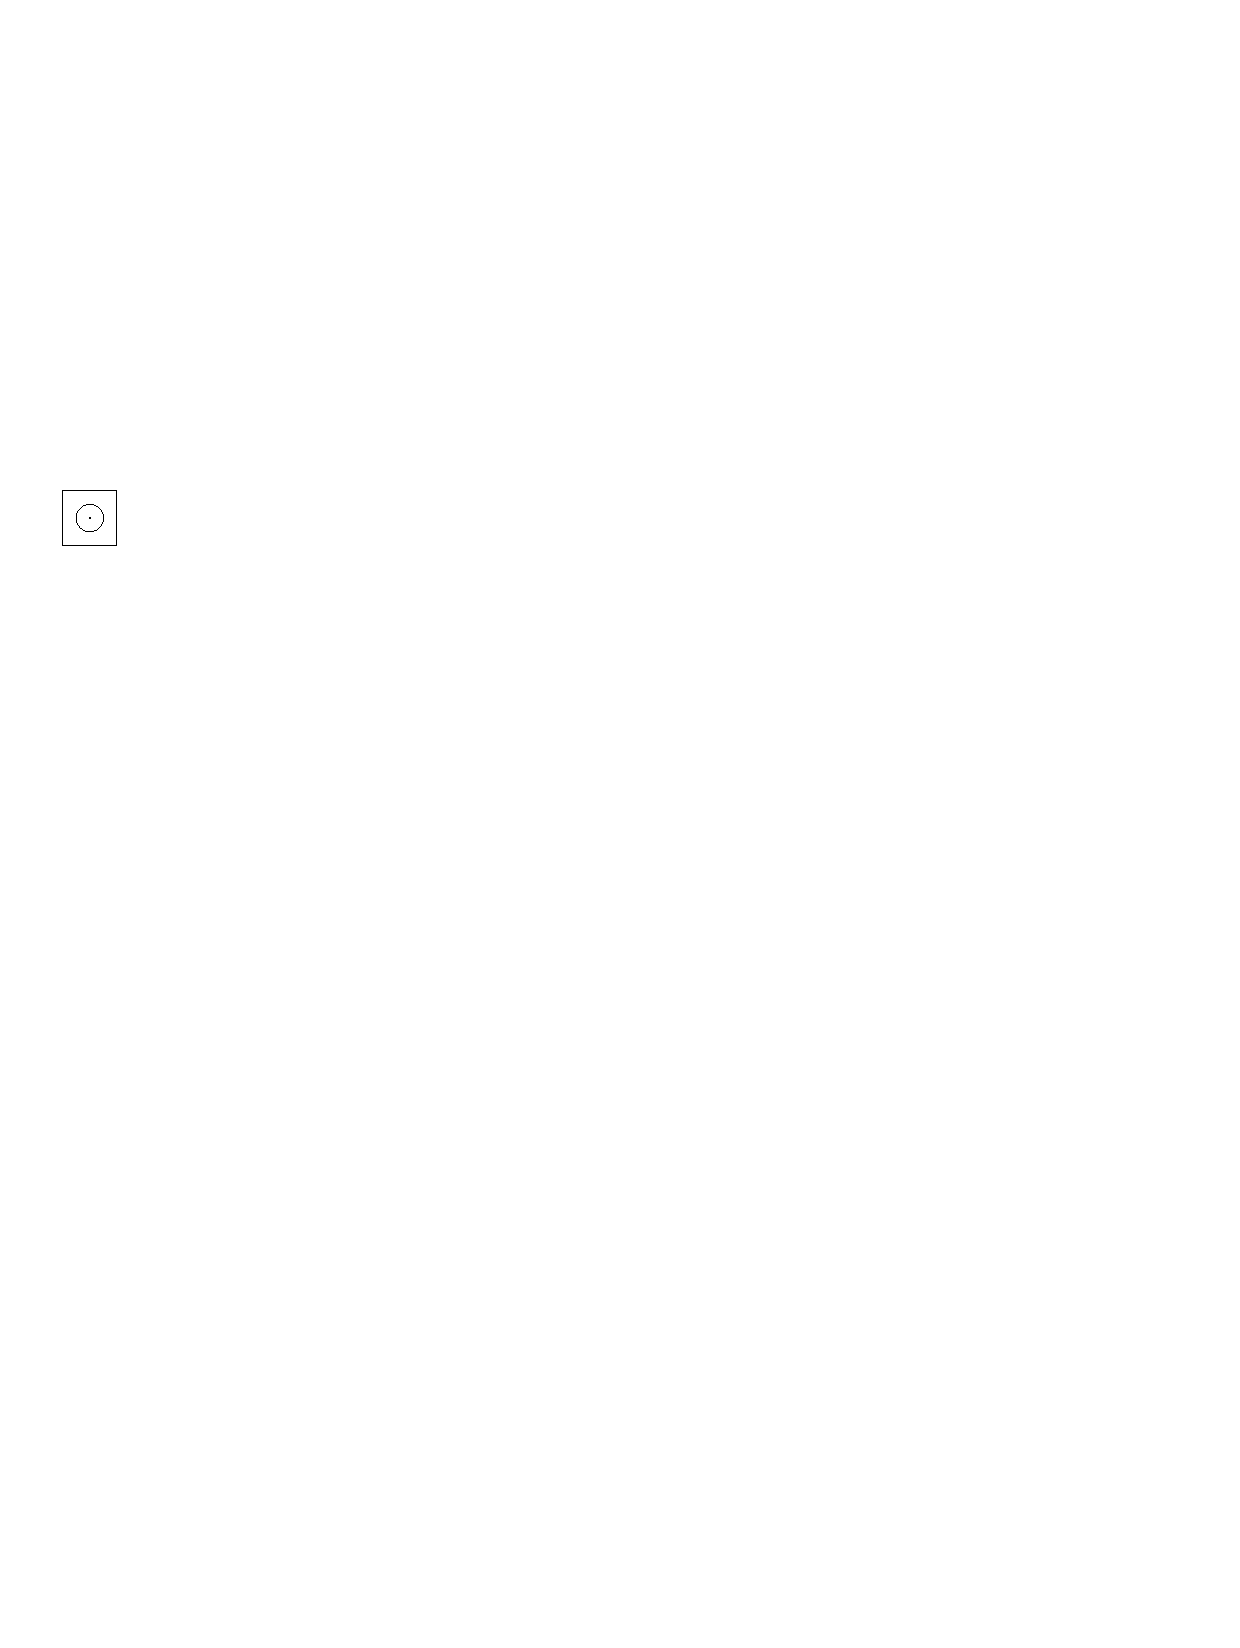
\includegraphics[scale=2]{img/sez_urto_p10}
\end{wrapfigure}
cada dentro il cerchietto è pari alla probabilità che questa particella venga diffusa. Quindi si può immaginare che una particella incidente subirà diffusione se cadrà dentro il cerchietto. La sezione d'urto viene anche detta \textit{sezione efficace di diffusione}. Nel caso limite di urto classico, $\sigma$ coincide con le dimensioni della particella bersaglio. Questo in realtà non si può mai verificare perché le particelle possono interagire senza venire a contatto.

Nella diffusione si possono avere sia diffusioni elastiche che anelastiche contemporaneamente (cioè alcune particelle subiscono diffusione elastica e altre anelastica). In questo caso si dice che la diffusione avviene secondo due canali. In questo caso $W$ è la somma sia di quella elastica che quella anelastica, cioè
\begin{equation}
 W = W_{\text{el}} + W_{\text{anel}}
\end{equation}
dove $W_{\text{el}}$ e $W_{\text{anel}}$ sono definite analogamente a $W$. Ovviamente si ha
\[
W_\text{el} = \sigma_\text{el}I n_b;\qquad W_\text{anel} = \sigma_\text{anel}I n_b
\]
\begin{align*}
 \sigma_\text{el} &= \text{sezione d'urto elastica}\\
 \sigma_\text{anel} &= \text{sezione d'urto anelastica}
\end{align*}
Essendo
\[
 W = \sigma I n_b \Rightarrow
\]
\begin{empheq}[box=\fbox]{equation}
 \sigma = \sigma_\text{el} + \sigma_\text{anel}
\end{empheq}

Un altro modo di definire la sezione d'urto è
\begin{align*}
N &= \text{numero di particelle diffuse nell'unità di tempo}\\
A_b &= \text{area della superficie bersaglio}\\
N &= W A_b
\end{align*}
Quindi si può scrivere
\[
N = \sigma I n_b A_b \Rightarrow N = \sigma I N_b
\]
dove $N_b$ è il numero totale di particelle bersaglio. Questo modo di definire $\sigma$ è comodo quando $N_b = 1$, infatti si avrà
\begin{empheq}[box=\fbox]{equation}
 \sigma = \frac{N}{I}
\end{empheq}
Questa è \textit{la probabilità che una singola particella incidente venga diffusa dal bersaglio}.

La frequenza di diffusione $W$ può anche interpretarsi come \textit{attenuazione d'intensità del fascio incidente}. Infatti $n = -\delta n_i$ che è il numero di particelle che il fascio incidente perde per unità di tempo per unità di superficie. Quindi
\[
n = -\delta n_i \Rightarrow \delta I = \delta n_i \Rightarrow
\]
\begin{empheq}[box=\fbox]{equation}
 W = -\delta I
\end{empheq}

\breaknote
Consideriamo\marginnote{17-11-1997} ora\footnote{Qui manca una frase che essenzialmente ripeteva quanto detto un rigo sopra, in quanto cambiando il giorno la lezione si riallaccia a quella precedente. \`E stata rimossa per migliorare la scorrevolezza. [NdT]} un fascio incidente che attraversa uno strato di materia. Sia $\Delta x= x- x_0$ lo spessore di questo strato e $\rho_b$ la densità di volume delle particelle bersaglio. Sia $I(x_0) = I(0)$ l'intensità iniziale del fascio incidente. Per calcolare $I(x)$ basta suddividere lo strato di spessore $\Delta x$ in strati infinitesimi di spessore $dx$. Il numero di particelle bersaglio per unità di area è $\rho_bdx$. La variazione di intensità dovuta al singolo strato è
\[
dI = -dW = -\sigma I \rho_bdx
\]
Si suppone che $\sigma$ non dipenda da $x$, cioè tutti gli strati hanno la stessa sezione d'urto. Integrando l'equazione si ha che
\[
\int\limits^{I(x)}_{I(0)} \frac{dI}{I} = -\int\limits^x_0 \sigma \rho_b dx \Rightarrow \ln[I(x)] - \lg[I(0)] = -\sigma\rho_b x \Rightarrow I(x) = I(0)e^{-\sigma\rho_bx}
\]
Si può anche scrivere nella forma
\begin{empheq}[box=\fbox]{equation}
 I(x) = I(0)e^{-\mu x}; \qquad \mu = \sigma\rho_b
\end{empheq}
$\mu$ si dice \textit{coefficiente di assorbimento} e ha le dimensioni di un inverso di una lunghezza. Da questa legge si determina che \textit{se $x\gg 1/\mu$, $I(x)$ diventa trascurabile}. Ad esempio i raggi cosmici non riescono a penetrare la crosta terrestre. Invece per i neutrini il coefficiente $\mu$ è molto piccolo e quindi un fascio di neutrini può attraversare tutta la terra senza subire grossa attenuazione. La sezione d'urto di solito si misura in \textit{barn} con la definizione
\begin{equation}
 1\text{ barn} = 10^{-24}\text{cm}^2
\end{equation}

Si è detto che la sezione d'urto totale si definisce come $\sigma = \sigma_\text{el} + \sigma_\text{anel}$. Analizziamo ora la probabilità che la diffusione avvenga in una particolare direzione. Consideriamo la direzione $(\theta,\phi)$ e l'angolo solido $d\Omega = \sin\theta d\theta d\phi$ e consideriamo il numero di particelle\footnote{Per coerenza con quanto detto prima, il numero di particelle si intende \textit{per unità di superficie e tempo}.} $dn$ che vengono diffuse\footnote{Sia elasticamente che anelasticamente. } nella direzione dell'angolo solido $d\Omega$. $dn$ sarà sempre proporzionale all'intensità del fascio incidente e alla densità di particelle bersaglio. Si può definire la frequenza
\[
dW = dn(\theta,\phi) = d\sigma(\theta,\phi)In_b = dW(\theta,\phi)
\]
moltiplicando e dividendo per $d\Omega$ si può scrivere\footnote{$d\sigma(\theta,\phi)$ è la sezione d'urto differenziale. }
\begin{equation}
dW = \frac{d\sigma}{d\Omega}In_bd\Omega
\end{equation}

Ovviamente deve esistere il legame con la sezione d'urto totale\footnote{Integrando sull'angolo solido. }
\begin{equation}
 \sigma = \int\limits^{4\pi}_0\frac{d\sigma}{d\Omega}d\Omega
\end{equation}
$\frac{d\sigma}{d\Omega}$ si può valutare\footnote{Come la $\sigma$ si distribuisca al variare dell'angolo solido. } sperimentalmente\footnote{Con contatori di particelle diffuse da spostare ai vari angoli. }. Si può sempre scrivere
\[
\frac{d\sigma}{d\Omega} = \frac{d\sigma_\text{el}}{d\Omega} + \frac{d\sigma_\text{anel}}{d\Omega}
\]

Consideriamo il caso in cui si abbia solo una particella bersaglio\footnote{In generale, se $N_b$ è il numero totale di particelle bersaglio $d\sigma = dN/(IN_b)$. }. Anche in questo caso si può definire la sezione d'urto differenziale
\[
d\sigma = \frac{dN}{I}, \qquad N_b = 1
\]
dove $dN$ è il numero di particelle incidenti che vengono diffuse nell'unità di tempo in un dato angolo solido $d\Omega$. Questa formula si può applicare al caso di una diffusione dovuta al potenziale elettrostatico\footnote{Modello di Rutherford. } generato da una carica fissa\footnote{$I$ è un flusso di particelle che si estende all'infinito. }.

L'importanza della diffusione è dovuta a due motivi: uno è che le interazioni della fisica nucleare e subnucleare  sono sempre a corto raggio e le sezioni d'urto possono fornire informazioni sulla struttura del bersaglio\footnote{Informazioni date dagli urti. }; il secondo motivo è che lo studio dettagliato di una interazione a corto raggio è molto più problematico rispetto a interazioni a raggio infinito. La trattazione è \textit{sempre quantistica e non esiste un corrispondente classico}, quindi l'analisi della sezione d'urto\footnote{Lo studio è abbastanza difficile. } è uno dei pochi strumenti che si hanno per studiare queste interazioni\footnote{Natura e meccanismo delle interazioni in gioco. }.

\section{Processi di decadimento}


Supponiamo che in un certo volume siano presenti delle particelle che hanno una certa probabilità di decadere. Supponiamo che queste particelle siano \textit{un insieme statistico}. Sia $N(t)$ il numero di particelle non ancora decadute al tempo $t$ e supponiamo che questo $N(t)$ sia sufficientemente grande in modo che si possa trattare come una grandezza continua (cioè $\lvert \delta N\rvert = 1 \ll N(t)$). All'istante $t + dt$ si avranno $N(t+dt)$ particelle non ancora decadute. Il numero di decadimenti nell'intervallo di tempo $dt$ è
\[
-dN(t) = N(t) - N(t+dt)
\]

La \textit{frequenza di decadimento} si definisce come
\begin{empheq}[box=\fbox]{equation}
 F(t) = -\frac{dN(t)}{dt}
\end{empheq}
questa rappresenta il numero di decadimenti nell'unità di tempo. Determiniamo ora la funzione $F(t)$ trattando i decadimenti come eventi casuali. Quindi il numero di decadimenti è proporzionale ad $N(t)$ con un coefficiente di proporzionalità che\footnote{Per l'omogeneità del tempo. } non può dipendere dal tempo. Quindi si può porre
\[
F(t) = -\frac{dN(t)}{dt} = \lambda N(t)
\]
$\lambda$ si dice \textit{costante di disintegrazione}\footnote{La probabilità di decadimento nell'unità di tempo. } (è l'analogo della sezione d'urto nei processi di diffusione). Ha le dimensioni di $t^{-1}$. Questa rappresenta la probabilità di decadimento nell'unità di tempo, cioè
\[
\lambda = -\frac{dN/dt}{N} = \textit{cost.}
\]
Tutto questo vale perché abbiamo fatto l'ipotesi di casualità dei decadimenti. Integrando l'equazione differenziale trovata per $N$ si ottiene che:
\begin{empheq}[box=\fbox]{equation}
 N(t) = N(0)e^{-\lambda t}
\end{empheq}
Da questa si ha
\begin{empheq}[box=\fbox]{equation}
 F(t) = \lambda N(0)e^{-\lambda t}
\end{empheq}
Questa legge esponenziale sembra essere valida per tutti i decadimenti\footnote{Quindi $F(t)$ non è una costante e ha un massimo per $t=0$. }

\section{Tempo di vita media}
Consideriamo\marginnote{19-11-1997}\footnote{Per la prima volta viene
  identificato il periodo storico del secondo Discente Ignoto, artefice degli
  Appunti negli Appunti. Infatti, accanto la data del '97 ne viene riportata una
  seconda: \textit{19/03/2007}.} sempre un volume in cui sono presenti delle
  particelle identiche che hanno una certa probabilità di decadere ($\lambda
$). Si definisce il \textit{tempo di vita media} di una particella
\begin{empheq}[box=\fbox]{equation}
 \tau = \frac{1}{\lambda}
\end{empheq}

Verifichiamo che effettivamente la vita media di una particella sia $1/\lambda$.
Consideriamo delle particelle che vivono da $0$ a $t$. Queste sono le particelle
che decadono nell'intervallo di tempo che va da $t$ a $t+dt$. Quindi si ha che
\[
dN'(t) = -dN(t) = \lambda N(t)dt = \lambda N(0)e^{-\lambda t}dt
\]
Questo è il numero di particelle che hanno vita pari a $t$. Per definizione la
vita media di una particella è
\begin{equation}
 \bar{t} = \frac{1}{N(0)}\int\limits^{+\infty}_0tdN'(t) = \frac{1}{N(0)}\int\limits^{+\infty}_0t\lambda N(t)dt = \int\limits^{+\infty}_0t\lambda e^{-\lambda t}dt = \frac{1}{\lambda} = \tau
\end{equation}

Si può verificare che se la frequenza di decadimento fosse costante ed uguale al
valore iniziale (cioè $F = \lambda N(0)=$ cost.) in questo caso $\tau$
rappresenterebbe il tempo in cui tutte le particelle sarebbero decadute. Infatti
\[
\int\limits^{N(t)}_{N(0)}dN = -\lambda N(0)t\Rightarrow N(t) = N(0)(1-\lambda t)
\]
Quindi si avrebbe $N(t) > 0$ per $t<\tau$ e $N(t) = 0$ per $t=\tau$.

Consideriamo il grafico della funzione $N(t)$ (\autoref{fig:decadimento_p15}):
\begin{enumerate}
 \item questa curva rappresenta $N(t) = N(0)e^{-\lambda t}$;
 \item questa curva rappresenta $N(t) = N(0)(1-\lambda t)$
\end{enumerate}
\begin{figure}[htbp]
\centering
\caption{Grafico delle due funzioni $N(t)$ considerate.}
\label{fig:decadimento_p15}
\begin{tikzpicture}[line cap=round,line join=round,>=stealth
  ,x=3.331070320176694cm,y=2.697038194702317cm]
  \draw[->,color=black] (-0.14,0) -- (2.56,0);
  \foreach \x in {,0.2,0.4,0.6,0.8,1,1.2,1.4,1.6,1.8,2,2.2,2.4}
  \draw[shift={(\x,0)},color=black] (0pt,2pt) -- (0pt,-2pt);
  \draw[->,color=black] (0,-0.17) -- (0,1.68);
  \foreach \y in {,0.2,0.4,0.6,0.8,1,1.2,1.4,1.6}
  \draw[shift={(0,\y)},color=black] (2pt,0pt) -- (-2pt,0pt);
  \clip(-0.14,-0.17) rectangle (2.56,1.68);
  \draw[smooth,samples=100,domain=0.0:2.5574449791162808]
  plot(\x,{2.718281828^(2*(\x)-4*(\x))});
  \draw[smooth,samples=100,domain=0.0:0.5] plot(\x,{1-2*(\x)});
  \draw (-0.09,1.68) node[anchor=north] {$N$};
  \draw (0.03,1.11) node[anchor=north west] {$N_0$};
  \draw (0.47,0.51) node[anchor=north west] {$1$};
  \draw (0.3,0.32) node[anchor=north] {$2$};
  \draw (0.48,0.03) node[anchor=north west] {$\tau$};
  \draw (2.03,-0.01) node[anchor=north west] {$t$};
  \begin{scriptsize}
	\fill [color=\MinorColor] (0,1) circle (1.5pt);
	\fill [color=\MinorColor] (0.5,0) circle (1.5pt);
  \end{scriptsize}
\end{tikzpicture}

\end{figure}
Quindi graficamente è possibile determinare $\tau$ considerando l'intersezione
con l'asse delle $x$ della retta tangente a $N(t) = N(0)e^{-\lambda t}$ nel
punto $t=0$. Definiamo\marginnote{Tempo di dimezzamento} ora il \textit{tempo di
dimezzamento}, cioè il tempo in cui il numero di particelle non decadute è
uguale alla metà del numero iniziale di particelle. Se indichiamo con $T$ il
tempo di dimezzamento si deve avere
\begin{equation}
 N(T) = \frac{1}{2}N(0) = N(0)e^{- T/\tau} \Rightarrow \frac{1}{2} = e^{-T/\tau} \Rightarrow T = \ln(2)\tau\approx 0.69\tau
\end{equation}

Tutte queste considerazioni teoriche sono una buona approssimazione della realtà
se la velocità delle particelle sono piccole rispetto a $c$, cioè se si è fuori
da ambiti relativistici\footnote{Oppure particelle ferme.}.

Vediamo ora come si definiscono questi parametri nel caso in cui le particelle
hanno una velocità $v$ non trascurabile rispetto a $c$. Quindi per $t$ e $T$ si
ha\footnote{Dipendono dal tipo di decadimento (interazione) e dalla velocità.}
\begin{align}
 \tau(v) &= \frac{\tau(0)}{\sqrt{1-v^2/c^2}}\\
 T(v) &= \frac{T(0)}{\sqrt{1-v^2/c^2}}
\end{align}
$\tau(v)$ è la vita media nel sistema in cui le particelle sono a velocità $v$,
$\tau(0)$ è la vita media nel sistema di riferimento in cui le particelle sono
ferme. Lo stesso vale per $T(v)$ e $T(0)$ e per $\lambda(v)$ e $\lambda(0)$. Per
$\lambda$ si ha
\begin{equation}
 \lambda(v) = \lambda(0)\sqrt{1-v^2/c^2}
\end{equation}
Quindi se una particella\footnote{Ad esempio i \textit{muoni}. } ha una vita
media piccola, se questa particella si trova a velocità $v\approx c$ la sua vita
media può aumentare notevolmente\footnote{$\tau$ è minimo nel \textsc{SR}
solidale alle particelle. }.

\chapter{Cenni di relatività}
\section{Energia cinetica relativistica}
I processi dinamici nucleari e subnucleari sono governati dalla legge $E_0 = mc^2$ dove $m$ è la massa a riposo. Se l'oggetto è in moto questa legge diventa
\[
E(v) = \frac{mc^2}{\sqrt{1-v^2/c^2}} = \gamma mc^2
\]
dove si è definito $\gamma = 1/\sqrt{1-v^2/c^2}$. Ovviamente $E(v=0) = E_0$. L'espressione $E(v)$ contiene l'energia totale dell'oggetto. Quindi $E(v)$ è la somma dell'energia cinetica e dell'energia a riposo, quindi si può scrivere
\begin{empheq}[box=\fbox]{equation}
T = E(v) - E_0 = mc^2(\gamma(v)-1)
\end{empheq}

Se $v\ll c$ si trova $T \approx \frac{1}{2}mv^2$. Questo risultato si ottiene sviluppando $\gamma (v)$ in serie di potenze di $v/c$, cioè arrestandosi al secondo ordine
\[
\gamma(v) \approx 1 + \frac{1}{2}\frac{v^2}{c^2}
\]
Quest'espressione di $T(v)$ si può trovare equivalentemente dal teorema dell'energia cinetica\footnote{$T$ = lavoro di una forza esterna per portare un corpo da $v =0$ a $v=v_0$. }. In fisica nucleare e subnucleare l'energia si esprime di solito in MeV\footnote{Un elettronvolt è l'energia cinetica di un elettrone accelerato da una differenza di potenziale pari a un volt. [NdT]} (1 eV = \SI{1.6e-19}{J} = \SI{1.6e-12}{erg}). Valutiamo ad esempio l'energia a riposo dell'elettrone, del protone e del neutrone in \autoref{tab:en_riposo}.
\begin{table}[htbp]
\centering
\caption{Energie a riposo di elettrone, protone e neutrone.}
\label{tab:en_riposo}
\begin{tabular}{cS[table-format=3.1]}
\toprule
Particella & {Energia (MeV)}\\
\midrule
$m_ec^2$ & 0.5\\
$m_pc^2$ & 938.2\\
$m_nc^2$ & 939.5\\
\bottomrule
\end{tabular}
\end{table}

La definizione relativistica di quantità di moto è
\begin{empheq}[box=\fbox]{equation}
 \vec{P} = \gamma(v) m\vec{v}
\end{empheq}
e di solito si indica $\gamma m$ \textit{massa effettiva} o massa relativistica. L'energia e la quantità di moto sono le componenti di un quadrivettore nello spazio di Minkowski\footnote{Lo spazio con la metrica descritta da $ds^2 = (cdt)^2 - dx^2 - dy^2 - dz^2$. }. Il modulo quadro di questo vettore è
\begin{empheq}[box=\fbox]{equation}
 P^2 = \frac{E^2}{c^2} - p^2;\qquad \vec{P} \equiv (\frac{E}{c}, \vec{p}) \tag{Quadrimpulso della particella}
\end{empheq}
dove si è adottata la metrica $ds^2 = (cdt)^2 - dx^2 - dy^2 - dz^2$. Sappiamo che i \textit{moduli di quadrivettori sono invarianti}\footnote{Restano invarianti per rotazioni, ovvero per cambiamento del SR. }, quindi $P^2 = \text{cost.}$ al variare del SR. Nel sistema in cui la particella è ferma si ha che $P^2 = E^2/c^2 = m^2c^2$. Quindi si ha \textit{sempre}
\begin{empheq}[box=\fbox]{equation}
 P^2 = \frac{E^2}{c^2} - p^2 = m^2c^2
\end{empheq}

Il fattore adimensionale $\gamma (v)$ rappresenta un utile parametro per valutare se è necessario o meno usare una trattazione relativistica. Il caso classico si ha per $\gamma = 1$, quindi se consideriamo il parametro $\gamma - 1$ questo ci da una stima dell'errore relativo che si ha usando una trattazione non relativistica. Infatti
\[
\gamma - 1 = \frac{\gamma m - m}{m}
\]
che è un errore relativo sulla massa.

\breaknote
Dalla\marginnote{21-11-1997} definizione relativistica dell'energia cinetica segue che il parametro $\gamma -1$ si può anche scrivere come
\begin{empheq}[box=\fbox]{equation}
 \gamma - 1 = \frac{T}{E_0} = \frac{\text{energia cinetica}}{\text{energia a riposo}}
\end{empheq}
Ad esempio in fisica nucleare per l'elettrone si ha
\[
T_e: [1\text{MeV}, 10\text{MeV}]
\]
quindi per l'elettrone si deve usare una trattazione relativistica. Infatti si ha
\[
0.2 \leq \gamma - 1 \leq 20
\]

Per il protone ed il neutrone energie cinetiche fino a 10MeV consentono una trattazione classica, infatti si ha 
\[
\gamma - 1  \lesssim 0.01 = 1\%
\]

\section{Energia di soglia}
Passiamo ora al concetto di \textit{energia di soglia}. Consideriamo un processo
dinamico in cui particelle più leggere si uniscono per dare origine a particelle
più pesanti. Vediamo in questo caso l'importanza del principio di equivalenza
fra massa ed energia. Consideriamo una particella $M$ bersaglio e una particella
$m$ che collide con $M$ ($m<M$ sono masse a riposo). Sia $M'$ la massa del
sistema che si genera dall'unione di $m$ e $M$. Questo sistema può essere
costituito da una sola particella o da $n$ particelle $M_1', M_2',...,M_n'$.
In questo caso la massa $M'$ si definisce come
\begin{equation}
 M' = \frac{E_\text{CM}}{c^2}; \qquad E_\text{CM} = \text{energia nel sistema del centro di massa}
\end{equation}

In generale, così definito $M'$, si ha che
\begin{equation}
 M' \geq M_1' + \cdots + M_n' > m+M
\end{equation}
L'eguaglianza si ha solo se le $M_i'$ sono tutte a riposo. Infatti in generale si ha
\begin{empheq}[box=\fbox]{equation}
 M' = E_\text{CM}/c^2 = \gamma(v_{1,\text{CM}}')M_1' + \cdots + \gamma(v_{n,\text{CM}}')M_n'; \qquad \gamma(v_{i,\text{CM}}) \geq 1
\end{empheq}
Dato quindi un processo di reazione di questo tipo si dice energia di soglia del processo l'energia minima $E_s$ che la particella incidente di massa $m$ deve avere affinché avvenga questo determinato processo. L'energia di soglia ovviamente deve essere tale che $M'$ assuma il suo valore minimo, cioè deve essere
\[
M' = M_1' + \cdots + M_n'
\]
Questa è la definizione di $E_s$. Vediamo adesso come si calcola.

Consideriamo il quadrimpulso delle particelle iniziali. Il suo modulo è
\begin{equation}
\label{eq:p_mod}
P^2_\text{tot} = \frac{(E + Mc^2)^2}{c^2} - p^2 = \frac{E^2}{c^2} + M^2c^2 + 2EM - p^2 = m^2c^2 + M^2c^2 + 2EM
\end{equation}
dove
\begin{itemize}
 \item[$p$] è il momento di $m$;
 \item[$E$] è l'energia di $m$;
 \item[$Mc^2$] è l'energia di $M$.
\end{itemize}
Da questo si vede che $P^2_\text{tot}$ è funzione solo di $E$. Consideriamo ora il modulo quadro del quadrimpulso finale
\[
P^{'2}_\text{tot} = M^{'2}c^2
\]
Per la conservazione del modulo quadro del quadrimpulso si deve avere che
\[
P^2_\text{tot}(E) = P^{'2}_\text{tot} = M^{'2}c^2
\]
Il valore di $E_s$ è quello tale che
\[
P^2_\text{tot}(E) = M^{'2}_\text{min}c^2 = (M_1' + \cdots + M_n')^2c^2
\]
e in forma esplicita, confrontata con \eqref{eq:p_mod}, questa equazione dà
\begin{empheq}[box=\fbox]{equation}
\label{eq:en_soglia}
 E_s = \frac{M^{'2}_\text{min} - M^2 - m^2}{2M}c^2
\end{empheq}
Nel caso particolare in cui il sistema finale sia costituito da una sola particella di massa $M'$ si ha
\[
E_s = \frac{M^{'2} - M^2 - m^2}{2M}c^2
\]

Applichiamo il concetto di energia di soglia al processo di formazione di una coppia elettrone-positrone. Ad esempio consideriamo la reazione
\begin{equation}
 \gamma + N \rightarrow e^+ + e^- + N
\end{equation}
dove $N$ è un nucleo. La presenza di $N$ \textit{è necessaria per garantire la conservazione della quantità di moto}. Infatti, se $N$ non fosse presente, si avrebbe
\[
\vec{P}_\text{in} = \vec{P}_\gamma \neq 0;\quad \vec{P}_\text{fin} = \vec{P}_{e^-} + \vec{P}_{e^+} = 0
\]
$\vec{P}_\text{fin}$ è nullo perché ci siamo posti nel sistema del centro di massa della coppia elettrone-positrone.

Calcoliamo ora l'energia di soglia relativa a questo processo. Sia $M_N$ la massa del nucleo, $m_e$ la massa del positrone e dell'elettrone. Nella \eqref{eq:en_soglia} si devono fare le seguenti sostituzioni
\[
M = M_N;\quad M'_\text{min} = M_N + 2m_e;\quad m = m_\gamma = 0
\]
Da queste si ottiene
\begin{equation}
 E_s = \frac{(M_n + 2m_e)^2 - M_N}{2M_N}c^2 = 2m_ec^2\left[1+\frac{m_e}{M_N}\right]
\end{equation}
Questa è l'energia minima che un fotone deve avere affinché da un urto con un nucleo si generi una coppia elettrone-positrone. Dall'espressione si deduce che $E_s > 2m_ec^2$ che è l'energia a riposo della coppia $e^+$-$e^-$. Questo è dovuto al fatto che dopo l'urto si avrà una energia cinetica sia del nucleo che di $e^+$ ed $e^-$. Però dal momento che $M_N\gg m_e$ si ha praticamente $E_s \approx 2m_ec^2$. Quindi le particelle $e^+$ ed $e^-$ sono strettamente a riposo rispetto al nucleo. Al limite si può assumere che la massa del nucleo sia infinita in modo che il nucleo non acquisti energia cinetica ed $E_s = 2m_ec^2$. In questa approssimazione la coppia $e^+$-$e^-$ è ferma. Se l'energia $E$ iniziale è maggiore di $E_s$ si ha un'energia cinetica della coppia $e^+$-$e^-$. Se $E$ continua ad aumentare si arriverà all'energia di soglia per il processo di creazione di due coppie elettrone-positrone.

\section{Energia di legame e difetto di massa}
Un'altra\marginnote{24-11-1997} conseguenza del principio di equivalenza fra
massa ed energia è il legame tra difetto di massa ed energia di legame. Sia $M$
la massa di una particella. Supponiamo che $M$ decada spontaneamente in due
particelle di massa $m_1$ e $m_2$. Per quanto detto prima si deve avere
\begin{align*}
M &> m_1 + m_2\\
Mc^2 &= \gamma(v_1) m_1c^2 + \gamma(v_2) m_2c^2
\end{align*}
Questo nel caso in cui $M$ decada spontaneamente. Supponiamo ora che $M$ sia
stabile e cioè non decada spontaneamente. Si definisce \textit{energia di
legame} l'energia minima che si deve fornire affinché $M$ si scinda in $m_1$ e
$m_2$. Definiamo le energie a riposo
\begin{equation}
 E_0 = Mc^2;\quad E_{01} = m_1c^2; \quad E_{02} = m_2c^2
\end{equation}
Se $\Delta E_0$ è l'energia di legame si deve avere per definizione
\begin{equation}
\Delta E_0 + E_0 = E_{01} + E_{02} \Rightarrow \Delta E_0 = (E_{01} + E_{02}) - E_0
\end{equation}
Per ipotesi deve essere $E_0 > 0$, quindi $E_0 < E_{01} + E_{02}$. A questo
punto applichiamo l'equivalenza fra massa ed energia e si può dedurre che $M <
m_1 + m_2$.

Quindi la \textit{particella $M$ stabile} ha massa inferiore alla somme delle
masse delle particelle che la compongono. Si definisce \textit{difetto di massa}
\begin{equation}
 \Delta M = (m_1 + m_2) - M = \text{Difetto di massa}
\end{equation}
e ovviamente
\begin{equation}
\Delta M = \frac{\Delta E_0}{c^2}
\end{equation}
Questo risultato trova applicazione nei nuclei stabili. \textit{La massa di un
nucleo stabile è minore delle masse di protoni e neutroni che lo compongono}.
Consideriamo ad esempio il nucleo d'elio
\[
  2m_p + 2m_n \approx 3755 \ \dfrac{\text{MeV}}{c^2}
\]
mentre il valore sperimentale della massa del nucleo d'elio è
\begin{align*}
M_\text{He} &\approx 3727\text{MeV/c}^2\\
\Delta M &\approx 28\text{MeV/c}^2 \Rightarrow \Delta E_0 \approx 28\text{MeV}
\end{align*}
Quindi misurando la massa di un nucleo si può dedurre $\Delta E_0$ e quindi le forze che tengono uniti i nucleoni.

\chapter{Cenni di meccanica quantistica}

\section{Statistiche di Fermi-Dirac e Bose-Einstein}

Se $\psi(\vec{r},t)$ è la funzione d'onda di una particella, allora
$\abs{\psi(\vec{r},t)}^2d^3r$ è la probabilità che all'istante $t$ la particella
si trovi nel volumetto $d^3r$ centrato nel punto $\vec{r}$. Questa funzione
$\psi(\vec{r},t)$ è soluzione dell'equazione di Schr\"odinger
\begin{equation}
 i\hslash \frac{\partial}{\partial t}\psi(\vec{r},t) = H \psi(\vec{r},t)
\end{equation}

Consideriamo due particelle, 1 e 2, e sia $\psi(1,2,t)$ la funzione d'onda. Se
non consideriamo lo spin questa si può scrivere come $\psi(\vec{r}_1, \vec{r}_2,
t)$. Se le due particelle non sono interagenti si ha
\[
H(1,2) = H(1) + H(2)
\]
ovvero l'hamiltoniana del sistema è uguale alla somma delle hamiltoniane delle
due particelle. Per quanto detto si avrà che
\[
\psi(1,2,t) = \psi_a(1,t)\cdot \psi_b(2,t)
\]
dove $\psi_a$ e $\psi_b$ sono soluzioni dell'equazione di Schr\"odinger con
$H(1)$ e $H(2)$. La funzione $\psi_a$ rappresenta lo stato quantistico della
particella 1 e $\psi_b$ lo stato della particella 2. In \textit{generale}
$\psi_a \neq \psi_b$. Per quanto definito si avrà per la probabilità
\[
\abs{\psi(1,2,t)}^2\cdot d^3r_1\cdot d^3r_2 = \abs{\psi(1,t)}^2d^3r_1\cdot
\abs{\psi(2,t)}^2d^3r_2
\]
Questa è la probabilità di trovare simultaneamente la particella 1 in
$\vec{r}_1$ e la particella 2 in $\vec{r}_2$. Quanto fatto ha senso se le due
particelle sono distinguibili l'una dall'altra. Solo in questo caso infatti si
può porre una corrispondenza biunivoca $1\leftrightarrow\psi_a$ e
$2\leftrightarrow\psi_b$. Questa corrispondenza perde di significato quando le
particelle sono identiche in quanto \textit{dal punto di vista quantistico sono
indistinguibili, a meno che le loro funzioni d'onda non siano definite in domini
spaziotemporali con intersezione nulla}. Quando questo non avviene le particelle
sono indistinguibili.

Analizziamo le conseguenze di questa indistinguibilità mantenendo però valida
l'ipotesi di due particelle non interagenti. Sia $\psi(1,2,t)$ la loro funzione
d'onda. Deve essere che
\[
\psi(1,2,t) \neq \psi_a(1,t)\psi_b(2,t)
\]
perché non si può stabilire quale particella si trovi nello stato $\psi_a$ e
quale nello stato $\psi_b$. Cioè la funzione d'onda deve contenere
contemporaneamente i termini $\psi_a(1,t)\psi_b(2,t)$ e
$\psi_a(2,t)\psi_b(1,t)$. Introduciamo \textit{l'operatore di scambio} $P_{1,2}$
il cui unico effetto è quello di scambiare le due particelle (cioè le loro
coordinate), cioè si definisce
\begin{equation}
\begin{rcases}
P_{1,2}\psi(1,2,t) &= \psi(2,1,t)\\
P_{1,2} \psi_i(1,t) &= \psi_i(2,t)\\
P_{1,2} \psi_i(2,t) &= \psi_i(1,t)
\end{rcases}\text{con }i=a,b
\end{equation}
Se applichiamo questo operatore, questo \textit{non potrà provocare alcun
cambiamento osservabile}. Quindi deve essere
\[
\abs{\psi(1,2,t)}^2 = \abs{\psi(2,1,t)}^2
\]
Questa uguglianza implica che
\[
P_{1,2}\psi(1,2,t) \equiv \psi(2,1,t) = \eta\psi(1,2,t)\qquad\text{con }\abs{\eta}^2 = 1
\]
Poiché l'assegnazione dei numeri 1 e 2 è puramente convenzionale deve essere
verificata la relazione
\[
P_{1,2}\psi(2,1,t) \equiv \psi(1,2,t) = \eta\psi(2,1,t)
\]
Da queste due si deduce che $\eta^2=1\Rightarrow\eta=\pm 1$. Per la funzione
d'onda $\psi$ si può porre in definitiva che
\begin{equation}
\psi(1,2,t)\propto[\psi_a(1,t)\psi_b(2,t) + \eta\psi_a(2,t)\psi_b(1,t)]
\end{equation}

\breaknote
Nel\marginnote{26-11-1997} caso in cui le particelle identiche siano interagenti
non sarà più possibile scrivere le loro funzioni d'onda in forma fattorizzata,
questo perché l'Hamiltoniana in questo caso è del tipo
\[
H(1,2) = H(1) + H(2) + V(1,2)
\]
Continua però a sussistere l'indistinguibilità, quindi deve essere sempre
verificato che
\[
P_{1,2}\psi(1,2,t) \equiv \psi(2,1,t) = \eta\psi(1,2,t)\qquad\text{con }\eta =\pm 1
\]
Si può concludere in modo generale che \textit{la funzione d'onda di due
particelle identiche è simmetrica o antisimmetrica rispetto allo scambio delle
coordinate}. Questa è infatti una proprietà intrinseca, rimane cioè invariata
nel tempo. Infatti si ha
\begin{align*}
 \psi(1,2,t+dt) &= \psi(1,2,t) + \frac{\partial}{\partial t}\psi(1,2,t)dt\\
 i\hslash \frac{\partial}{\partial t}\psi(1,2,t) &= H \psi(1,2,t)
\end{align*}
e $H$ è ovviamente invariante \textit{per lo scambio delle due particelle}, cioè
$H(1,2) = H(2,1)$. Tenuto conto di questa proprietà segue dall'equazione di
Schr\"odinger
\begin{equation}
 i\hslash \frac{\partial}{\partial t}\psi(2,1,t) = H \psi(2,1,t) = \eta H \psi(1,2,t) = \eta i\hslash \frac{\partial}{\partial t}\psi(1,2,t)
\end{equation}
Quindi $\frac{\partial}{\partial t}\psi(2,1,t) = \eta \frac{\partial}{\partial
t}\psi(1,2,t)$. Da queste considerazioni si deriva che $\eta$ \textit{non può
essere funzione del tempo}. Quando $\eta = 1$ si dice che le due particelle
identiche obbediscono alla \textit{statistica di Bose-Einstein}; quando $\eta =
-1$ le due particele identiche obbediscono alla \textit{statistica di
Fermi-Dirac}.
\begin{empheq}[box=\fbox]{align}
 \psi(1,2,t) &= \psi(2,1,t)\qquad\text{statistica di \textit{Bose-Einstein}}\\
 \psi(1,2,t) &=-\psi(2,1,t)\qquad\text{statistica di \textit{Fermi-Dirac}}
\end{empheq}

Le particelle del primo tipo si chiamano
\textit{bosoni}. Le particelle del secondo si chiamano \textit{fermioni}. Le
particelle del secondo tipo sono soggette al principio di esclusione di Pauli.
Infatti se due fermioni identici non interagenti\footnote{Se due particelle
  fossero invece interagenti, non avrebbe senso parlare di principio di Pauli in
  quanto non si potrebbe parlare di stato di \textit{una} singola particella.}
  avessero lo stesso stato quantico allora la loro funzione d'onda complessiva
  sarebbe
\[
\psi(1,2)\propto[\psi_a(1)\psi_b(2) - \psi_a(2)\psi_b(1)] \equiv 0
\]
Empiricamente sappiamo che si comportano come bosoni tutte le particelle che
hanno spin pari a un multiplo intero di $\hslash$. Quando lo spin è un multiplo
semi-intero di $\hslash$ le particelle si comportano come fermioni.

Consideriamo adesso un insieme di $N$ particelle identiche non interagenti. Il
generico stato in cui una particella può trovarsi sia
$\psi_{k_i}\;(i=1,\dots,N)$. Se le particelle fossero distinguibili si potrebbe
assegnare a ciascuna di esse un ben determinato stato e la funzione complessiva
sarebbe
\[
\psi(1,\dots,N) = \psi_{k_1}(1)\psi_{k_2}(2)\cdots\psi_{k_N}(N)
\]
Se invece le particelle sono indistinguibili, uno o più scambi di particelle non
possono portare a cambiamenti del sistema. In questo caso deve essere verificato
che
\begin{equation}
 P_{ij}\psi_{k_i}(i)\psi_{k_j}(j) = \psi_{k_i}(j)\psi_{k_j}(i)
\end{equation}
Se si tratta di fermioni, la funzione complessiva sarà antisimmetrica per un
numero dispari di scambi e simmetrica per un numero pari di scambi. Se si tratta
invece di bosoni, la funzione d'onda complessiva sarà sempre simmetrica per un
numero qualsiasi di scambi effettuati.

Consideriamo l'insieme di indici $(1,2,\dots,N)$ e una generica permutazione
$P\equiv (P_1,P_2,\dots,P_N)$. Il numero delle possibili permutazioni è $N!$.
Ciascuna permutazione $P$ si ottiene dalla successione iniziale per mezzo di un
numero di scambi $n_P$. Quindi un sistema di $N$ particelle identiche non
interagenti, che siano dei fermioni, si può descrivere con una funzione d'onda
complessiva del tipo\footnote{I pedici $FD$ e $BE$ stanno per Fermi-Dirac e
Bose-Einstein rispettivamente. [NdT]}
\begin{equation}
 \psi_{FD} \propto \sum\limits_P(-1)^{n_P}\psi_{k_1}(P_1)\psi_{k_2}(P_2)\cdots\psi_{k_N}(P_N)
\end{equation}
Nel caso di bosoni invece si ha
\begin{equation}
 \psi_{BE} \propto \sum\limits_P\psi_{k_1}(P_1)\psi_{k_2}(P_2)\cdots\psi_{k_N}(P_N)
\end{equation}

Queste funzioni sono definite a meno di un fattore moltiplicativo. Per trovare
tale fattore basta considerare l'interpretazione probabilistica della funzione
d'onda. Assumiamo che le singole funzioni d'onda siano già normalizzate, cioè
\[
\int_V \abs{\psi_{k_i}(P_i)}^2d^3r_{P_i} = \int_V \abs{\psi_{k_i}(i)}^2d^3r_{i}
= 1
\]
Un'analoga condizione di normalizzazione deve valere per la funzione d'onda
complessiva, cioè deve essere verificato che
\[
\int_V \abs{\psi_{FD}}^2d^3r_1\, d^3r_2\,\cdots\, d^3r_N = \int_V
\abs{\psi_{BE}}^2d^3r_1\, d^3r_2\,\cdots\, d^3r_N = 1
\]
Facciamo l'ipotesi che sia $\psi_{k_i} \neq \psi_{k_j}$ per $i\neq j$, cioè che
gli stati siano tutti diversi. Questa ipotesi è obbligatoria se si considerano
fermioni identici. Comunque assumiamo questo vero anche se le particelle sono
bosoni. Sotto queste ipotesi vale anche una condizione di ortonormalità fra gli
stati, cioè
\[
 \int_V \psi^*_{k_i}(P_i)\psi_{k_j}(P_i)\, d^3r_{P_i} = \int_V
 \psi^*_{k_i}(i)\psi_{k_j}(i)\, d^3r_{i} = \delta_{ij}
\]
Tenuto conto di queste considerazioni, la condizione di normalizzazione della
funzione d'onda complessiva risulta verificata se si pone
\begin{empheq}[box=\fbox]{align}
 \psi_{FD} &=
 \frac{1}{\sqrt{N!}}\sum\limits_P(-1)^{n_P}\psi_{k_1}(P_1)\psi_{k_2}(P_2)\cdots\psi_{k_N}(P_N)\\
 \psi_{BE} &= \frac{1}{\sqrt{N!}}\sum\limits_P\psi_{k_1}(P_1)\psi_{k_2}(P_2)\cdots\psi_{k_N}(P_N)
\end{empheq}
Nel caso in cui $N=2$, cioè se si hanno solo due particelle identiche, si ha che
\begin{align}
 \psi_{FD} &= \frac{1}{\sqrt{2}}[\psi_{k_1}(1)\psi_{k_2}(2) - \psi_{k_1}(2)\psi_{k_2}(1)]\\
 \psi_{BE} &= \frac{1}{\sqrt{2}}[\psi_{k_1}(1)\psi_{k_2}(2) + \psi_{k_1}(2)\psi_{k_2}(1)]
\end{align}
ricordando che questi fattori di noralizzazione ($1/\sqrt{N!}$) valgono sotto
l'ipotesi di stati tutti differenti.

\section{Funzione d'onda di una particella che decade}

In\marginnote{28-11-1997} meccanica quantistica lo stato di una particella
libera con quantità di moto ed energia ben definite si dice \textit{stato
stazionario} e la funzione d'onda che lo descrive è
\begin{equation}
 \phi(\vec{r},t) = \phi(\vec{r})\psi(t)\qquad\text{dove }\phi(\vec{r})\propto e^{\frac{i}{\hslash}\vec{p}\cdot\vec{r}}\quad\text{e}\quad\psi(t) = \psi(0)e^{-\frac{i}{\hslash}Et}
\end{equation}
Se la particella è a riposo $E=E_0=mc^2$, con $m$ massa della particella.
Ovviamente si ha che
\[
\abs{\psi(t)}^2 = \abs{\psi(0)}^2 = \text{costante}
\]
Supponiamo di normalizzare la funzione d'onda $\phi(\vec{r},t)$ in modo tale che
\[
\int_V\abs{\phi(\vec{r},t)}^2\, d^3r = \int_V\abs{\phi(\vec{r})}^2\, d^3r =
1\quad\text{dove si è posto }\abs{\psi(0)}^{2}=1
\]
$\abs{\psi(t)}^2 = \abs{\psi(0)}^2 = 1$ si interpreta come la probabilità che la
particell esista nel volume $V$ all'instante $t$. Essendo questa uguale a 1, la
particella risulta stabile.

\textit{Se invece la particella non fosse stabile non potrebbe essere}
$\abs{\psi(t)}=1$ verificata ad ogni $t$, quindi lo stato della particella non
potrà essere uno stato stazionario. Per il principio di indeterminazione tra
tempo ed energia deve essere
\[
\Delta E = \hslash/\tau
\]
dove $\tau$ è la vita media della particella. Questo è in accordo col fatto che
la particella non è in uno stato stazionario.

Si ha però che lo stato di una particella che decade si può in genere
approssimare ad uno \textit{stato quasi stazionario}. Cioè si può assumere che
l'andamento temporale della funzione d'onda sia
\begin{equation}
 \psi(t) = \psi(0)e^{-\frac{i}{\hslash}Et}
\end{equation}
dove però $E$ è una quantità complessa. In particolare si ha
\begin{empheq}[box=\fbox]{equation}
 E = \bar{E} - i\frac{\Gamma}{2}
\end{empheq}
dove $\bar{E}$ e $\Gamma$ sono numeri positivi. Con queste considerazioni la
funzione d'onda si può scrivere
\begin{equation}
 \psi(t) = \psi(0)\exp\left[-\frac{i}{\hslash}\bar{E}t - \frac{1}{2\hslash}\Gamma t\right]
\end{equation}
In questo caso si vede che la $\psi(t)$ è sostanzialmente diversa da quella
dello stato stazionario. Si vede che quanto più $\Gamma$ è piccolo, tanto più lo
stato si avvicina ad uno stato stazionario. Dal momento che
\[
E\longrightarrow\bar{E}\qquad\text{per }\Gamma\longrightarrow 0
\]
si può interpretare $\bar{E}$ \textit{come il valore medio dell'energia}, cioè l'energia può assumere valori nell'intervallo
\begin{equation}
 \left[\bar{E} - \frac{\Delta E}{2};\;\bar{E} + \frac{\Delta E}{2}\right]
\end{equation}
dove $\Delta E$ è l'incertezza data dal principio d'indeterminazione. In particolare \textit{se la particella è a riposo $\bar{E}$ ci da il valore medio della massa della particella}. Quindi \textit{una particella instabile non ha una massa ben definita}.

Consideriamo adesso la quantità $\Gamma$. Il modulo quadro di $\psi(t)$ è 
\begin{equation}
 \abs{\psi(t)}^2=\abs{\psi(0)}^2e^{-\frac{\Gamma}{\hslash}t} = e^{-\frac{\Gamma}{\hslash}t}
\end{equation}
dove si è posto $\abs{\psi(0)}^2 = 1$. $\abs{\psi(t)}^2$ ci deve sempre dare la probabilità che la particella esista al tempo $t$ nel volume $V$.

Per un insieme statistico di particelle identiche instabili sappiamo che il numero di particelle non ancora decadute all'istante $t$ è
\begin{equation}
 N(t) = N(0)e^{-\lambda t}
\end{equation}
quindi si può porre, per il significato probabilistico di $\abs{\psi(t)}^2$
\begin{equation}
 \abs{\psi(t)}^2 = N(t)/N(0)
\end{equation}
Da questa segue che
\[
e^{-\Gamma t/\hslash} = e^{-\lambda t}
\]
ovvero
\begin{empheq}[box=\fbox]{equation}
 \label{eq:largh_lvl_en}
 \Gamma = \hslash\lambda = \hslash/\tau = \Delta E
\end{empheq}
Tenendo conto del principio di indeterminazione si interpreta $\Gamma$ come l'indeterminazione minima dell'energia di una particella che decade. $\Gamma$ viene detta \textit{larghezza del livello energetico di una particella}. \`E logico aspettarsi che l'approssimazione di stato quasi stazionrio sia buona quando $\Gamma\ll\bar{E}$, cioè quando è possibile assegnare un valore di energia abbastanza preciso.

Questa condizione può essere vista anche sotto un altro aspetto, infatti possiamo scrivere
\begin{equation}
 \tau = \hslash/\Gamma \gg \hslash/\bar{E} = \bar{T}
\end{equation}
dove $\bar{T}2\pi$ è il periodo medio caratteristico di oscillazione della funzione d'onda della particella. Di conseguenza \textit{si può parlare di stato quasi stazionario quando la vita media della particella è molto più grande del periodo di oscillazione della funzione d'onda}.

Il decadimento di una particella può avvenire teoricamente o in un unico modo oppure in modi diversi. Ad esempio un atomo che si trova ad un livello energetico eccitato può avere un unico modo di decadere se esiste un solo livello più basso, mentre se esistono più livelli inferiori il decadimento può avvenire in modi diversi, con diversi stati finali.

Consideriamo il caso generale in cui siano $n$ il numero di possibili modi di decadere, ciascuno di questi caratterizzati dalla costante $\lambda_i(i=1,\dots,n)$. Si dice che in questo caso la particella ha $n$ canali di decadimento e $\lambda_i$ la probabilità di decadere nell'unità di tempo per il canale i-esimo. In questo caso si ha
\begin{equation}
 \lambda = \sum_i\lambda_i
\end{equation}
Per ciascun canale si può definire una larghezza parziale
\begin{equation}
 \Gamma = \hslash \lambda = \sum_i\Gamma_i
\end{equation}

Consideriamo un insieme statistico di particelle identiche con $n$ canali di decadimento. Si ha che
\begin{equation}
\frac{\Gamma_i}{\Gamma} = \frac{\lambda_i}{\lambda}
\end{equation}
è la percentuale di decadimenti nell'i-esimo canale. Questo si dice \textit{rapporto di diramazione} (= ``branching ratio''). Si definiscono pure i tempi parziali di vita media
\begin{equation}
 \tau_i = 1/\lambda_i
\end{equation}
Questi però possono contribuire all'effettivo tempo di vita media secondo la relazione
\begin{equation}
 \tau = 1/\lambda\Rightarrow \frac{1}{\tau} = \sum_i\frac{1}{\tau_i}\Rightarrow\tau<\tau_i\quad\forall i = 1,\dots,n
\end{equation}

%!TEX root = nucleare.tex
% fino a pag circa 41
\section{Spazio di Hilbert}

Supponiamo \marginnote {1-12-1997}
di avere un sistema quantistico costituito da una particella puntiforme e
descritto da una funzione d'onda scalare.
Sia essa $\phi(\vec{r},t)$. Il sistema risulta definito all'istante \textit{t}
da questa funzione. Poniamo:
$\phi(\vec{r},t) =\phi_{p}(t)$
dove $p$ è il punto individuato da $\vec{r}$. Quindi l'insieme dei valori
${\phi(t)}$ descrive ed individua il nostro sistema.

Lo stato all'istante $t$ si può geometricamente rappresentare come un
\textit{vettore appartenente ad uno spazio di dimensione infinita} le cui
componenti siano le $\phi_{p}(t)$. Questo spazio si dice \textit{Spazio di
Hilbert} o spazio degli stati ed i corrispondenti vettori si dicono vettori
dello stato.

Un generico vettore di questo spazio si indica con:

\begin{equation}
 \ket{t}  \qquad \text{KET}
\end{equation}%(nota dell'autore: "picciò˜ non ho idea di come si faccia, spero sia venuto bene, ah e non so manco mettere le note!")

questo descrive lo stato del sistema all'istante $t$.
Supponiamo ora che all'istante $t$ il sistema sia localizzato in un certo punto
$p'$ (cioè la funzione d'onda è nulla in tutti i punti diversi da $p'$), quindi
si ha:

\[
\phi_{p}(t)=0 \quad \text{per } p\neq p'
\]

Il ket che individua questo stato si indica con 
$\ket{\vec{r'},t}$

Consideriamo ora l'insieme di tutti questi ket al variare di $\vec{r'}$, questa
è una buona base o un insieme completo, dello spazio di Hilbert. Questa base è
ortogonale.

Per quanto detto un generico ket $\ket{t}$ si può esprimere in funzione della
base ortogonale $\ket{\vec{r'},t}$, quindi le componenti $\phi_{p}(t)$  sono
ortogonali e si ha che:
\begin{equation}
\int \psi^*_{p}(t)\psi_{p}(t) d^3\vec{r}= \int \psi^*(\vec{r},t)\psi(\vec{r},t)d^3\vec{r}%la formula è uguale a quella degli appunti...
\end{equation}
cioè il modulo quadro del vettore $\ket{t}$ è la somma (integrale) dei moduli
quadri delle componenti.

Si definisce anche il prodotto scalare fra due stati partendo dal fatto che il
modulo quadro di $\ket{t}$ si può interpretare come il prodotto scalare con se
stesso. Questo si indica con:
\begin{equation}
\braket{t|t} \quad \text{dove} \bra{t} \text{  si dice BRA}
\end{equation}

Quindi ad ogni vettore $\ket{t}$ si associa il suo duale $\bra{t}$ e si ha la
corrispondenza biunivoca\footnote{Sotto certe condizioni. }:
\begin{equation}
\ket{t}\equiv \{\psi_{p}(t)\}\longrightarrow \bra{t} \equiv\{\psi^*_{p}(t)\}
\end{equation}

Quindi il prodotto scalare fra il vettore $\ket{t,a}$ e $\ket{t,b}$ si definisce
come:
\begin{equation}
\braket{t,b|t,a}=\int\psi^{*(b)}_p(t)\psi^{(a)}_p(t) d^3\vec{r}
\end{equation}

Per quanto definito si ha che:
\begin{equation}
\braket{t,a|t,b}=\braket{t,b|t,a}^*
\end{equation}

Due vettori si dicono ortogonali quando il loro prodotto scalare è nullo.
Ovviamente la condizione di ortogonalità dovrà valere per i vettori di base.
Questi vettori di base possono essere definiti in modo che la base risulti
ortonormale, questo, per definizione, significa che:
\begin{equation}
\psi_p(t)\equiv \braket{\vec{r},t|t}
\end{equation}
cioè quando per una base succede questo la base si dice ortonormale.

Se $\ket{t}$ è lo stato che descrive il nostro sistema e se questo stato è
normalizzato, cioè $\braket{t|t}=1$, allora si ha che:
\begin{equation}
|\braket{\vec{r},t|t}|^2=\psi^*(\vec{r},t)\psi(\vec{r},t)
\end{equation}
Questa è la densità di probabilità trovare la particella nel punto$\vec{r}$
all'istante $t$. Il generico $\ket{t}$
 si può esprimere in funzione della base, secondo la formula:
 
\begin{equation}
\ket{t}= \int{\psi_{p}\braket{\vec{r},t}d^3\vec{r}}=\int{\braket{\vec{r},t|t}}\ket{\vec{r},t}d^3\vec{r}
\end{equation}

Determiniamo quale condizione devono soddisfare i vettori di base affinché
effettivamente la base risulti ortonormale. Deve essere verificato che:

\begin{equation}
\braket{\vec{r},t|t}=\int{\psi _{p}(t) \braket{\vec{r}',t
|\vec{r},t}d^3\vec{r}}=\psi_{p'}(t)
\end{equation}
da questa segue:

\begin{empheq}[box=\fbox]{equation}
\braket{\vec{r},t|\vec{r},t}=\delta^3(\vec{r}-\vec{r'})
\end{empheq}

Con questa posizione i vettori di base risultano automaticamente ortogonali, la $\delta^3$ si può esprimere nella forma fattorizzata:
\begin{equation}
\delta^3(\vec{r}-\vec{r'})=\delta(x-x')\delta(y-y')\delta(z-z')
\end{equation}
\breaknote

Tutte \marginnote{3-12-1997} le grandezze osservabili sono rappresentate da operatori  \textit{hermitiani} che agiscono sui Ket.
A questi operatori si associano matrici (anch'esse hermitiane) di dimensione infinita.

Si ha che:
\begin{equation}
A\ket{t,1}=\ket{t,2}
\end {equation}
dove $A$ è l'operatore hermitiano e $\ket{t,1}$ e $\ket{t,2}$ sono due Ket le cui componenti sono:
\begin{align}
\ket{t,1}&=\int\psi_{p}^{(1)}(t)\ket{\vec{r},t}d^3\vec{r}\\
\ket{t,2}&=\int\psi_{p}^{(2)}(t)\ket{\vec{r},t}d^3\vec{r}
\end{align}

Per definizione si ha:
\begin{equation}
\psi_{p'}(t)=\braket{\vec{r'},t|t,2}=\braket{\vec{r'},t|A|t,1}=
 \int\psi_{p}^{(1)}(t)\braket{\vec{r'},t|A|\vec{r},t}d^3\vec{r}=
 \int\psi_{p}^{(1)}(t)A_{p'p}d^3\vec{r}
\end{equation}
 dove si è posto:
 \begin{equation}
 A_{p'p}=\braket{\vec{r'},t|A|\vec{r},t}\qquad \textit{Elementi di matrice di A}
 \end{equation}
 
Così definiti gli elementi di matrice sono relativi alla base.
Quando si cambia base questi in genere cambiano. Se si prende come base quella degli autovalori di A allora l'espressione matriciale assume forma diagonale, con gli elementi reali. 
In generale lo spettro degli autovalori di un operatore può essere sia discreto, sia continuo.
\subsection{Spettro discreto}
$a_{k}$ sia l'autovalore, $\ket{a_{k},t}$ sia il corrispondente autostato (per semplicità si assume che non vi sia degenerazione).

Quindi, per definizione, si ha:

\begin{equation}
A\ket{a_{k},t}=a_{k}\ket{a_{k},t}
\end{equation}

Un generico stato $\ket{t}$ si potrà scrivere come:

\begin{equation}
\ket{t}=\sum_{k}c_{k}(t)\ket{a_{k},t}
\end{equation}
e con la normalizzazione $\braket{a_{k},t|a_{k'},t}=\delta_{kk'}$ si ha che :

\begin{equation}
c_{k}(t)=\braket{a_{k},t|t}
\end{equation}

La quantità:

\begin{equation}
|\braket{a_{k},t|t}|^2=|c_{k}(t)|^2
\end{equation}
fornisce la probabilità che una misura della grandezza A fornisca il valore $a_{k}$ quando il sistema si trova nello stato$ \ket{t}$.

La quantità:
\begin{equation}
\braket{t|A|t}     \qquad \textit{Valore medio o valore di aspettazione}
\end{equation}
si dice valore medio di A rispetto allo stato$\ket{t}$. Si verifica facilmente che:

\begin{equation}
\braket{t|A|t}=\sum_{k}|\braket{a_{k},t|t}|^2a_{k}= \sum_{k}|c_{k}|^2a_{k}
\end{equation}

\subsection{Spettro continuo}
Sia $a$ l'autovalore e $\ket{a,t}$ il corrispondente autovettore. Un generico ket $\ket{t}$ si potrà scrivere come:

\begin{equation}
\ket{t}=\int\braket{a,t|t}\ket{a,t}da
\end{equation}

\begin{equation}
\braket{a,t|a',t}=\delta(a-a')
\end{equation}

\begin{equation}
|\braket{a,t|t}|^2=P(a)
\end{equation}

L'ultima quantità scritta rappresenta la densità di probabilità della distribuzione degli autovalori relativa allo stato $\ket{t}$. Cioè la probabilità di ottenere con una misura un valore compreso tra $a$e $a+da$ è data da $|\braket{a,t|t}|^2$.

\subsection{Spettro quasi continuo}
Definiamo ora la situazione di spettro quasi continuo. Consideriamo un sistema
che sia confinato in un volume grande ma finito e tale che una funzione d'onda
assuma valori uguali sulla frontiera di questo insieme. Sotto queste ipotesi si
può passare dal caso continuo al caso discreto:

\begin{equation}
a \longleftrightarrow a_k
\end{equation}

\begin{equation}
\int|\braket{a,t|t}|^2da \longleftrightarrow \sum_{k}|\braket{a_{k},t|t}|^2
\end{equation}
cioè si ha il passaggio da una densità di probabilità ad una probabilità. La
distanza fra gli autovalori $a_k$si può rendere piccola aumentando il volume$V$
che racchiude il sistema. Per un $V$ fissato si può definire la densità di
autostato:
\begin{equation}
\rho(a_k)=\frac{\Delta n}{\Delta a_{k}}
\end{equation}
dove $\Delta n$ è il numero di autostati relativo all'intervallo $\Delta a_k$.
Con una opportuna scelta del volume $V$ gli autovalori possono essere trattati
come quantità continue, in quanto, la loro distanza risulta molto piccola. In
questo caso la densità di autostati diventa:
\begin{equation}
\rho(a_k)=\frac{\delta n}{\delta a_k}\quad \textit{con }\delta a_k\ll a_k
\end{equation}

Approssimando la quantità $\delta a_k$ ad un infinitesimo si dovrà parlare
quindi di probabilità di trovare un autovalore nell'intervallo di estremi
$a_k$ e $a_k+da_k$. Questa probabilità è:
\begin{equation}
|\braket{a_k,t|t}|^2\delta n
\end{equation}
dove $\delta n= \rho(a_k)\delta a_k$ è il numero di autostati i cui autovalori
sono compresi nell'intervallo $[a_k,a_k+\delta a_k]$. Con questa approssimazione
si ha:
\begin{equation}
\sum_k|\braket{a_k,t|t}|^2
\end{equation}
da cui:
\begin{equation}
\int|\braket{a_k,t|t}|^2\rho(a_k)\delta a_k
\end{equation}

Questa quindi è la riduzione di uno spettro continuo ad uno quasi continuo. In
pratica quello che si fa è l'approssimazione:

\begin{equation}
|\braket{a,t|t}|^2\simeq |\braket{a_k,t|t}|^2\rho(a_k)\delta a_k
\end{equation}

Ovviamente se si fa tendere $V$ ad infinito si deve avere:
\begin{equation}
\lim_{V\to\infty}|\braket{a_k,t|t}|^2\rho(a_k)\delta a_k = |\braket{a,t|t}|^2da
\end{equation}
L'utilità di questa approssimazione risulterà chiara quando si affronterà la teoria di Fermi.

\subsection{Operatore coniugato Hermitiano}
Sia $G$ un operatore lineare che agisce nello spazio di Hilbert. Si definisce $G^\dag$, \textit{operatore coniugato Hermitiano}, come:

\begin{gather}
\braket{t,2|G^{\dag}|t,1}=(\braket{t,1|G|t,2})^*\\
\ket{t,3}=G\ket{t,2}\\
\braket{t,2|G^{\dag}|t,1}=(\braket{t,1|G|t,2})^*=(\braket{t,1|t,3})^*=\braket{t,3|t,1}
\end{gather}
Quindi per $G^{\dag}$ e $G$ vale la proprietà:

\begin{equation}
\ket{t,3}=G\ket{t,2} \Longrightarrow \bra{t,3}=\bra{t,2}G^{\dag}
\end{equation}

Un operatore $G$ si dice \textit{Hermitiano} quando $G=G^{\dag}$. In questo caso se $\ket{g}$ è un autostato normalizzato di $G$ con autovalore $g$ si ha che:

\begin{equation}
\braket{g|G|g}=g 
\end{equation}

\begin{equation}
\braket{g|G^{\dag}|g}=g^*\rightarrow g=g*
\end{equation}
quindi gli autovalori di un operatore hermitiano sono tutti reali.

Un operatore $G$ si dice \textit{unitario} quando $G=G^{\dag}$\footnote{Il testo riporta così: $G=G^{-1}$}. Un operatore unitario conserva i moduli dei ket. Infatti:

\begin{equation}
\braket{t|G^{\dag}G|t}=\braket{t|t}
\end{equation}

Nel caso in cui lo spazio di Hilbert sia relativo ad un sistema di $N$ particelle i ket si scrivono come:

\begin{equation}
\ket{t}=\int\psi(\vec{r_1},\vec{r_2},\vec{r_3},...,\vec{r_N},t)\ket{\vec{r_1},\vec{r_2},\vec{r_3},...,\vec{r_N},t}d^3\vec{r_1}d^3\vec{r_2}...d^3\vec{r_n}
\end{equation}
dove si è posto $\ket{\vec{r_1},\vec{r_2},\vec{r_3},...,\vec{r_N},t}=\ket{\vec{r_1},t}\ket{\vec{r_2},t}...\ket{\vec{r_N},t}$.
Il prodotto scalare si definisce come:

\begin{equation}
\braket{t|t}=\int\psi^N(\vec{r_1},\vec{r_2},...,\vec{r_N},t)\psi(\vec{r_1},\vec{r_2},...,\vec{r_N},t)d^3\vec{r_1}...d^3\vec{r_N}
\end{equation}


\section{Rappresentazione di Schr\"{o}dinger}
Consideriamo un sistema quantistico descritto dalla funzione d'onda
$\psi(\vec{r},t)=\psi_{p}(t)$. Questa funzione soddisfa l'equazione di
Schr\"{o}dinger:

\begin{equation}
i\hslash\frac{\partial}{\partial t}\psi_{p}(t)=H\psi_{p}(t)
\end{equation}

Questa è equivalente all'equazione vettoriale:

\begin{equation}
i\hslash\frac{d}{dt}\ket{t}=H\ket{t}
\label{eq:rapp_Sch}
\end{equation}
con $\ket{t}=\int\psi_{p}(t)\cdot \ket{\vec{r},t}d^{3}\vec{r}$.
In realtà si è assunto che i vettori di base $\ket{\vec{r},t}$ non varino al
variare di $t$, cioè:
\begin{equation}
\frac{\partial}{\partial t}\ket{\vec{r},t}=0 
\end{equation}
se $\ket{\vec{r},t}=\ket{\vec{r}}$

La formulazione della meccanica quantistica basata sull'equazione
\eqref{eq:rapp_Sch} si dice \textit{rappresentazione di Schr\"{o}dinger}.

Esistono comunque altre rappresentazioni ed in particolare ne esistono un numero
infinito, tutte equivalenti. Questo perché non si possono misurare nè le
funzioni d'onda, nè gli operatori. Quello che si può misurare sono gli
autovalori e le probabilità associate.
Quindi ogni altra rappresentazione che lasci invariate queste due grandezze
andrà bene.
Se applichiamo una trasformazione unitaria a tutti gli elementi delllo spazio di
Hilbert si ottiene ad esempio una rappresentazione equivalente.
Questa trasformazione unitaria si definisce come:
\begin{equation}
  U\ket{t}=\ket{\vec{t}}  \text{ e } \bra{t}U^{\dag}=\bra{\vec{t}} \quad \text{con} UU^{\dag}=U^{\dagger}U=1
\end{equation}
Questa è una generica trasformazione unitaria. Definiamo:
\begin{equation}
U(A\ket{t})=\overrightarrow{A\ket{t}}=\vec{A}\ket{\vec{t}}
\end{equation}
dove $\vec{A}$ è l'operatore trasformato. Di questo si può dare una
rappresentazione esplicita:
\begin{equation}
\vec{A}\ket{\vec{t}}=UA\ket{t}=UAU^{\dag}U\ket{t}=UAU^{\dag}\ket{\vec{t}}
\end{equation}
quindi:
\begin{equation}
\vec{A}=UAU^{\dag}
\end{equation}

Se $A$ rappresenta una grandezza fisica e se $\ket{a_{k},t}$ è un suo autostato
con autovalore $a_{k}$ allora si ha che:
\begin{equation}
  \vec{A}\ket{\overrightarrow{a_{k}t}}=U(A\ket{a_{k}t})=a_{k}\ket{\overrightarrow{a_{k}t}}
\end{equation}
Quindi la trasformazione $U$ lascia invariati gli autovalori, e l'autostato di
$\vec{A}$ è il trasformato dell'autostato di $A$. Dal momento che:
\begin{equation}
\braket{\overrightarrow{a_{k}t}|\vec{t}}=\braket{a_{k}t|t}
\end{equation}
rimane invariata la probabilità di trovare in una misura l'autovalore $a_{k}$.
Abbiamo dunque dimostrato che questa è una rappresentazione equivalente.

Le rappresentazioni più comunemente usate sono quella di Heisenberg e quella di
interazione.

\section{Rappresentazione di Heisenberg}
Per introdurre questa rappresentazione partiamo dalla rappresentazione di
Schr\"{o}dinger. Consideriamo lo stato all'istante $t$.
Si può porre
\begin{equation}
\ket{t}= T (t,t_{0})\ket{t_{0}} 
\end{equation}
dove $T$ è l'operatore di sviluppo temporale e ovviamente $T(t_{0},t_{0})=1$.
Utilizzando l'equazione di Schr\"{o}dinger si verifica che:
\begin{equation}
i\hslash\frac{d}{dt}T=HT
\end{equation}
$T$ si può formalmente scrivere come:
\begin{equation}
T(t,t_{0})=\exp\left\{-\frac{i}{\hslash}H(t-t_{0})\right\}
\end{equation}
se $H$ è hermitiano allora $T$ risulta unitario. In queste ipotesi si conserva
la probabilità, infatti:
\begin{equation}
\braket{t|t}=\braket{t_{0}|T^{\dag}(t,t_{0})T(t,t_{0})|t_{0}}=\braket{t_{0}|t_{0}}
\end{equation}
nel caso quasi stazionario di un sitema che decade $H$ non è hermitiano, in
quanto ha autovalori complessi. In questo caso $T$ non è più unitario e non è
garantita la conservazione della probabilità. In ogni caso comunque $T$ commuta
con $H$, cioè:
\begin{equation}
[T,H]=TH-HT=0
\end{equation}
Quindi la rappresentazione di Heisemberg si ottiene considerando la
trasformazione unitaria:

\begin{empheq}[box=\fbox]{equation}
U=T^{\dag}(t,t_{0})=\exp\left\{\frac{i}{\hslash}H(t-t_{0})\right\}
\end{empheq}
cioè si deve applicare questa trasformazione alla rappresentazione di
Schr\"{o}dinger. Questo ovviamente si può fare solo se $H$ è hermitiana.
L'operatore $T^{\dag}$ verifica l'equazione:

\begin{equation}
-i\hslash\frac{d}{dt}T^{\dag}=T^{\dag}H=HT^{\dag}
\end{equation}
Il nuovo stato del sistema sarà:

\begin{equation}
\ket{\vec{t}}=T^{\dag}\ket{t}=\ket{t}_{H}=T^{\dag}T\ket{t_{0}}
\end{equation}
Inoltre si ha che:

\begin{equation}
\ket{t}_{H}=\ket{t_{0}}_{H}=\ket{t_{0}}
\end{equation}
da cui:

\begin{empheq}[box=\fbox]{equation}
\frac{d}{dt}\ket{t}_{H}=0
\end{empheq}

Quindi in questa rappresentazione lo stato rimane costante nel tempo, mentre
invece variano gli operatori. Supponiamo che l'operatore $A$ associato ad una
grandezza fisica non dipenda esplicitamente dal tempo. Dimostriamo che:

\begin{equation}
\frac{d}{dt}A=\frac{\partial}{\partial t}A=0
\end{equation}
Per ipotesi $\frac{\partial A}{\partial t}=0$.
Poniamo (rappresentazione di  Schr\"{o}dinger):

\begin{equation}
\begin{split}
\ket{t}=\int\psi_{p}(t)\ket{\vec{r}}d^{3}\vec{r} \\
A\ket{t}=\int\psi^{I}_{p}(t)\ket{\vec{r}}d^{3}\vec{r}
\end{split}
\end{equation}
dove:

\begin{equation}
\psi ^{I}_{p}(t)=\int A_{pp^{I}} \psi _{p^{I}}(t) d^{3} \vec{r}
\end{equation}
Derivando rispetto al tempo:

\begin{equation}
\begin{split}
\frac{d}{dt}\ket{t}=\int \frac{\partial}{\partial t}\psi_{p}(t)\ket{\vec{r}}d^{3}\vec{r}\\
\frac{d}{dt}[A\ket{t}]=\int\frac{\partial}{\partial t} \psi^{I}_{p}(t)\ket{\vec{r}}d^{3}\vec{r}
\end{split}
\end{equation}
dove si ha che:

\begin{equation}
\frac{\partial}{\partial t} \psi^{I}_{p}(t)=\int A_{pp^{I}} \frac{\partial}{\partial t} \psi_{p^{I}}(t)d^{3} \vec{r}
\end{equation}
Da tutto questo segue che:

\begin{gather}
\frac{d}{dt}[A\ket{t}]=A\frac{d}{dt}\ket{t} \rightarrow \frac{d}{dt}A=0
\end{gather}

Tutto questo è stato valutato nella rappresentazione di Schr\"{o}dinger. Vediamo
ora cosa succede nella rappresentazione di Heisenberg:

\begin{gather}
\vec{A}=A_{\mathscr{H}}=T^{\dagger}AT
\end{gather}

Valutiamo ora la derivata totale rispetto al tempo:

\begin{equation}
\begin{split}
\frac{d}{dt}A_{\mathscr{H}} &
=\left(\frac{d}{dt}T^{\dagger}\right)AT+T^{\dagger}A\left(\frac{d}{dt}T\right) \\
& = \frac{i}{\hslash}HT^{\dagger}AT-\frac{i}{\hslash}T^{\dagger}ATH \\
& = -\frac{i}{\hslash}(A_{\mathscr{H}}H-HA_{\mathscr{H}}) \\
& = -\frac{i}{\hslash}[A_{\mathscr{H}},H]
\end{split}
\end{equation}
Quindi l'operatore $A_{\mathscr{H}}$ verifica l'equazione:

\begin{empheq}[box=\fbox]{equation}
i\hslash \frac{d}{dt}A_\mathscr{H}=[A_\mathscr{H},H]
\end{empheq}
Questa vale nell'ipotesi che $\frac{\partial A}{\partial t}=0$. Se $A=H$ si ottiene che:

\begin{gather}
A_\mathscr{H}=H_\mathscr{H}=T^{\dag}HT=T^{\dag}TH=H\rightarrow H_\mathscr{H}=H
\end{gather}

Quindi anche nel sistema di Heisenberg:

\begin{equation}
\frac{d}{dt}H_\mathscr{H}=0
\end{equation}
se $\frac{\partial}{\partial t}H_\mathscr{H}=0$.

Il fatto che in questa rappresentazione lo stato di un sistema rimane costante implica che sono i vettori di base a variare nel tempo:

\begin{equation}
\begin{split}
\ket{\vec{r},t}_\mathscr{H} & =T^{\dag}(t,t_0)\ket{\vec{r}} \rightarrow \frac{d}{dt}\ket{\vec{r},t}_\mathscr{H} \\
& = \frac{d}{dt}T^{\dag}\ket{r} = \frac{i}{\hslash}H\ket{\vec{r},t}_\mathscr{H}
\end{split}
\end{equation}

Quindi i vettori $\ket{\vec{r} ,t}_\mathscr{H}$ variano nel tempo in modo esattamente opposto a come variano nel tempo i vettori nella rappresentazione di Schr\"{o}dinger.

\textit{In una qualsiasi rappresentazione vale sempre che} $\frac{\partial A}{\partial t}=0 \leftrightarrow \frac{d}{dt}A$. Nel caso della rappresentazione di Heisenberg si
 valuta $\frac{d}{dt}A_\mathscr{H}$ con l'ipotesi che sia $\frac{\partial A}{\partial t}=0 $ e non $\frac{\partial A_\mathscr{H}}{\partial t}=0 $.
 
\section{Rappresentazione di interazione}
Questa rappresentazione è molto usata nella fisica delle particelle elementari.
Consideriamo un generico sistema la cui Hamiltoniana viene posta nella forma:

\begin{equation}
H=H_{0}+H_\text{int}
\end{equation}
dove $H_0$ è il termine non perturbato e $H_\text{int}$ il termine di interazione. La
rappresentazione di interazione si ricava da quella di Schr\"{o}dinger
considerando la trasformazione unitaria:

\begin{empheq}[box=\fbox]{equation}
U = T_{0}^{\dag}(t,t_{0}) = e^{\frac{i}{\hslash}H_{0}(t-t_{0})}
\end{empheq}

Lo stato del sistema in questa rappresentazione diventa:

\begin{equation}
\ket{t}_I=T_{0}^{\dag}(t,t_{0})\ket{t}
\end{equation}
mentre un generico operatore si può scrivere come:

\begin{equation}
A_{I}=T_{0}^{\dag}(t,t_{0})AT_{0}(t,t_{0})
\end{equation}

Da questa definizione si nota subito che la rappresentazione di interazione è
una via di mezzo fra quella di Schr\"{o}dinger e quella di Heisemberg. In
particolare questa \textit{coincide con quella di Schr\"{o}dinger se $H_0=0$,
mentre coincide con quella di Heisenberg se $H_\text{int}=0$.}

Partendo dall'equazione di Schr\"{o}dinger e sostituendo $\ket{t}=T_0\ket{t}_I$
si ha:
\begin{equation}
\begin{split}
                      i\hslash \frac{\partial}{\partial t}\ket{t} &= H\ket{t} \\
               i\hslash \frac{\partial}{\partial t}(T_0\ket{t}_I) &= HT_0\ket{t}_I \\
HT_0\ket{t}_I + i\hslash T_0 \frac{\partial}{\partial t}\ket{t}_I &= (H_0+H_\text{int})T_0\ket{t}_I \\
                i\hslash T_0 \frac{\partial}{\partial t}\ket{t}_I &= H_\text{int}T_0\ket{t}_I \\
\end{split}
\end{equation}
e infine:

\begin{empheq}[box=\fbox]{equation}
i\hslash \frac{\partial}{\partial t}\ket{t}_I=(H_\text{int})_I\ket{t}_I
\end{empheq}

Questo significa che nella rappresentazione di interazione \textit{lo stato del
sistema varia nel tempo solo per effetto dell' Hamiltoniana di interazione.}

L'utilità di questa rappresentazione è evidente nello studio dei processi di
\textit{scattering}. Infatti con l'uso della rappresentazione di interazione è
possibile isolare la semplice evoluzione dinamica dallo stato iniziale allo
stato finale dopo lo scattering:

\begin{equation}
\ket{i}_I \rightarrow \ket{f}_I
\end{equation}

Questo discorso conserva la sua validità anche se il sistema è un sistema di
particelle.
Consideriamo ora un generico operatore $A$ che, nella rappresentazione di
Schr\"{o}dinger non dipende esplicitamente dal tempo, nella rappresentazione di
interazione invece varierà nel tempo solo per effetto di $H_0$:

\begin{equation}
\begin{split}
i\hslash \frac{\partial}{\partial t} A_I & = i\hslash \frac{\partial}{\partial
t}\left(e^{\frac{i}{\hslash}H_0(t-t_0)}Ae^{-\frac{i}{\hslash}H_0(t-t_0)}\right)=
\\
& =
i\hslash\left(\frac{i}{\hslash}H_0T_{0}^{\dag}AT_0-T_{0}^{\dag}A\frac{i}{\hslash}H_0T_0
\right)= \\
& = -H_0A_I+A_IH_0= \\
& = [A_I,H_0]
\end{split}
\end{equation}

Se consideriamo il caso in cui $A\equiv H_0$ si vede dall'espressione di $T_0$
che $H_{0_I}\equiv H_0$. Quindi $H_0$ è la stessa per la rappresentazione di
Schr\"{o}dinger  e di interazione. Lo stesso non vale in generale per
$H_\text{int}$ in quanto:
\begin{equation}
\begin{split}
[H_\text{int},H_0] &\neq 0 \Rightarrow \\
\Rightarrow H_{\text{int}_{I}} &\neq H_\text{int} \\
\Rightarrow \frac{\partial}{\partial t}H_{\text{int}_{I}} &\neq 0
\end{split}
\end{equation}
Tutto questo è evidente nei processi di scattering. Nella rappresentazione di
interazione lo stato iniziale $\ket{i}_I$ e quello finale $\ket{f}_I$ sono
indipendenti dal tempo in quanto si possono considerare imperturbati, cioè sono
autostati di $H_0$. Lo stato del sistema risulterà dipendente dal tempo solo
nell' intervallo di tempo in cui avverrà la transizione da $\ket{i}_I$  a
$\ket{f}_I$, ma questa transizione avviene ad opera di $H_\text{int}$, dunque
soltanto nel breve periodo della transizione $H_{int_{I}}$ può risultare diversa
da zero.

\section{Momento angolare}
Il momento angolare in meccanica quantistica è un operatore vettoriale $\vec{J}=
(J_x, J_y, J_z)$ le cui componenti verificano le seguenti regole di
commutazione:

\begin{gather}
[J_x, J_y]= i\hslash J_z\\
[J_y, J_z]= i\hslash J_x\\
[J_z, J_x]= i\hslash J_y
\end{gather}

Da queste regole di commutazione segue immediatamente che non può esistere un
autostato comune a $J_x, J_y$ e $J_z$ con autovalori non nulli.
In particolare non può esistere un autostato comune a due sole componenti con
autovalori non nulli. Infatti se esistesse uno stato che è autostato di $J_x$ e
$J_y$ allora dalla
prima regola di commutazione si vede che questo deve essere autostato di $J_z$
con autovalore nullo, ma dalle altre due regole di commutazione si deduce che
anche gli autovalori di $J_x$ e $J_y$ devono essere nulli.\footnote{l' unico
caso in cui l'autostato è autostato di $J_x, J_y, J_z$ è quello in cui $J=0$}

Si definisce l'operatore:

\begin{equation}
\vec{J}^2=J_{x}^2+J_{y}^2+J_{z}^2
\end{equation}
che rappresenta il modulo quadro di $\vec{J}$. Si possono facilmente verificare
le seguenti regole di commutazione:

\begin{gather}
[\vec{J}^2,J_x]= 0\\
[\vec{J}^2,J_y]= 0\\
[\vec{J}^2,J_z]= 0\\
\end{gather}

Risulta quindi che $\vec{J}^2$ commuta con ciascuna componente.
L'insieme di tutte queste regole di commutazione implica che lo stato del
sistema può essere contemporaneamente autostato di $\vec{J}^2$ e di una sola
delle componenti di
$\vec{J}$. L'asse individuato da tale componente si dice asse di
quantizzazione.\footnote{Tipo asse z}

Si può dimostrare che gli autovalori dell'operatore $\vec{J}^2$ sono:

\begin{equation}
j(j+1)\hslash^2
\end{equation}
dove: $j=0,\frac{1}{2},1,\frac{3}{2},2,\frac{5}{2}\dots$ Fissato un sottospazio
$j$ di $\vec{J}^2$ si ha che in questo sottospazio gli autovalori di $J_z$ sono:

\begin{equation}
m_j\hslash
\end{equation}
con $m_j=-j,-j+1,\dots,j-1,j$. Quindi il valore massimo che può avere $J_z$ è
$j\hslash$ e si  vede che il modulo quadro di $\vec{J}$ è più grande del
quadrato di $J_Z=j^2\hslash^2<j(j+1)\hslash^2$. Questo è conseguenza del fatto che
non può esistere uno stato del sistema in cui una delle componenti assume valore
massimo mentre le altre due assumono valore nullo.

Quindi supponendo che lo stato sia un autostato di $J_z$ quello con valore
massimo $j\hslash$
\begin{gather}
\braket{J_z}=j\hslash\\
\braket{J}=\braket{J_x}\vec{i}+\braket{J_y}\vec{j}+\braket{J_z}\vec{k}
\end{gather}
deve corrispondere al vettore classico:
\begin{equation}
\braket{J}=(0,0,j\hslash)
\end{equation}

Il modulo del vettore $\vec{J}$ è quindi pari a $j^2\hslash^2$. Se fosse
$\braket{J}\cdot \braket{J}=\braket{j^2}$ avremmo:
\begin{equation}
\braket{J^2}=\braket{J_x^2+J_y^2+J_z^2}=\braket{J_z}=j^2\hslash
\end{equation}

Ma quindi $\braket{J_x^2}=\braket{J_y^2}=0$ e lo stato sarebbe anche autostato
di $J_x$ e di $J_y$ con autovalore nullo.
\breaknote
Sia\marginnote{17/12/1997} $\ket{m_j}$ il generico autostato di $J_z$ e $J^2$,
quindi deve essere che:
\begin{equation}
J_z\ket{m_j}=m_j\hslash \ket{m_j}
\end{equation}
con 
\begin{equation}
m_j=-j,-j+1,\dots,j
\end{equation}

Quindi fissato $j$ il numero di autovalori corrispondenti di $J_z$ è $2j+1$
(questo sia per $j$ intero che semi-intero), ovviamente $2j+1$ è anche il numero
degli autostati
$\ket{m_j}$. Questi costituiscono una base degli stati con momento angolare $J$
fissato.

Apartire da $J_x$ e $J_y$ si definiscono gli operatori:

\begin{gather}
J_+ =J_x+iJ_y\\
J_- =J_x-iJ_y
\end{gather}
$J_+$ e $J_-$ sono uno il complesso coniugato dell'altro. Si verifica facilmente
che:

\begin{gather}
[J_z,J_+]=\hslash J_+ \\
[J_z,J_-]=-\hslash J_-
\end{gather}

Da queste regole di commutazione si può risalire al significato fisico dei due
operatori $J_+$ e $J_-$. Infatti si ha che:

\begin{equation}
\begin{split}
J_z(J_+\ket{m_j}) &= (\hslash J_++J_+J_z)\ket{m_j}=\\
& = \hslash J_+\ket{m_j}+\hslash m_j J_+\ket{m_j}=\\
& = \hslash(1+m_j)(J_+\ket{m_j})
\end{split}
\end{equation}

Quindi lo stato $J_+\ket{m_j}$ è uno autostato di $J_z$ con autovalore $\hslash
(m_j+1)$. Analogamente si dimostra che lo stato $J_-\ket{m_j}$ è un autostato di
$J_z$ con autovalore $\hslash(m_j-1)$. Quindi si può scrivere che:

\begin{gather}
J_+\ket{m_j}= \alpha \ket{m_j+1} \\
J_-\ket{m_j}= \beta \ket{m_j-1}
\end{gather}
con $-j<m_j<j$

Se consideriamo il caso in cui il nostro sistema è costituito da una singola
particella a riposo allora il momento angolare $\vec{J}$ si riduce all'
operatore $\vec{S}$, il momento
angolare di spin\footnote{Momento angolare intrinseco. }. In questo caso si
pone:
\begin{gather}
j=s \\
m_j=m_s=s,s-1,\dots,-s
\end{gather}
dove $s$ è il numero quantico di spin. Se la particella non è a riposo allora
$\vec{J}$ è la somma vettoriale del momento angolare orbitale e del momento di
spin.

%!TEX root = nucleare.tex
%DA PAG 41 A 61
Cioè si ha che: 
\begin{equation}
\vec{J} = \vec{L} + \vec{S}
\end{equation}
Se la particella non ha spin $\left( s = 0\right)$, $\vec{J}$ coincide con
$\vec{L}$ e, quindi, $j$ può assumere solo valori interi. Al posto di $j$ di
solito si usa $l$, che si dice numero quantico orbitale. \textit{Lo spin,
invece, è caratterizzato sia da valori interi che seminteri.}

Consideriamo ora il caso in cui si hanno due distinti momenti angolari,
$\vec{J_{1}}$ e $\vec{J_{2}}$, associati rispettivamente al sistema 1 e 2.
Supponiamo che sia:
\begin{equation}
\left[\vec{J_{1}}, \vec{J_{2}} \right] = 0
\end{equation}
cioè ogni componete di $\vec{J_{1}}$ commuta con ogni componente di
$\vec{J_{2}}$. Ogni autostato del sistema 1 sarà caretterizzato dai valori 
medi:
\begin{equation}
\mean{\vec{J_{1}}} = \left( \mean{J_{1x}}, \mean{J_{1y}}, \mean{J_{1z}} \right)
\end{equation}
e, ovviamente, anche per il sistema 2 si definisce:
\begin{equation}
\mean{\vec{J_{2}}} = \left( \mean{J_{2x}}, \mean{J_{2y}}, \mean{J_{2z}} \right)
\end{equation}
Si pone:
\begin{align}
\mean{\vec{J_{1}}} \cdot \mean{\vec{J_{1}}} &= j_{1}^{2}\hbar ^2 & 
\mean{\vec{J_{1}^{2}}} &= j_{1}\left(j_{1} +1\right)\hbar ^{2} \\
\mean{\vec{J_{2}}} \cdot \mean{\vec{J_{2}}} &= j_{2}^{2}\hbar ^2 & 
\mean{\vec{J_{2}^{2}}} &= j_{2}\left(j_{2} +1\right)\hbar ^{2} \\  
\end{align}
Definiamo l'operatore 
\begin{equation}
\vec{J} = \vec{J_{1}} + \vec{J_{2}}
\end{equation}
che è ancora un momento angolare: si possono verificare le regole di
commutazione per le sue componenti.

Si avrà che
\begin{align}
\mean{\vec{J}}\mean{\vec{J}} &= j^{2} \hbar ^{2} & \mean{\vec{J^{2}}} &= 
j\left(j+1\right)\hbar^2 
\end{align}
Si dimostra che fissati $j_{1}$ e $j_{2}$, $j$ può assumere solo dei valori ben
determinati, in quanto deve essere verificata la relazione
\begin{equation}
\abs{j_{1} - j_{2}} \leq j \leq j_{1} + j_{2} 
\end{equation}
Questa si dice anche \textit{condizione tringolare}. Questa stessa condizione si
può riscrivere nella forma:
\begin{equation}
\abs{j_{1} - j_{2}} \leq j = \left(m_{j}\right)_\text{\scshape max} \leq j_{1} 
+ j_{2}
\end{equation}
Ma si ha che il generico autovalore $m_{j}$ è dato da
\begin{equation}
m_{j} = m_{j_{1}} + m_{j_{2}}
\end{equation}
Quindi, essendo nota la variabilità di $m_{j_{1}}$ e $m_{j_{2}}$, si deduce che
\begin{equation}
j = j_{1} + j_{2}, j_{1} + j_{2}-1, \dots , \abs{j_{1} - j_{2}}
\end{equation}
Se $j_{1}<j_{2}$, sono $2j_{1} + 1$ valori. Se $j_{1}>j_{2}$, sono $2j_{2} + 1$
valori.

In meccanica classica si aveva già la condizione triangolare, la proprietà 
nuova
è che $j$ non può assumere tutti i valori fra il minimo ed il massimo. 

\textit{La degenerazione del sottospazio che si ottiene con $j_{1}$ e $j_{2}$
fissati è $\left(2j_{1} + 1\right)\left(2j_{2}+1\right)$}.

Consideriamo gli stati $m_{j}$, autostati di $\vec{J}^{2}$ e $J_{z}$. Si ha
sempre che, fissato $j$, si hanno $2j +1$ autostati. Questa molteplicità si 
dice
\textit{peso statistico} della stato con momento angolare $J$.

Fissati $j_{1}$ e $j_{2}$, il numero totale di stati è 
\begin{equation}
N = \sum _{j} \left(2j +1\right)
\end{equation}
con $j=\abs{j_{1} - j_{2}}, \dots , j_{1} +j_{2}$.
Se, ad esempio, $j_{1}<j_{2}$ la sommatoria è data da $2j_{1} + 1$ termini
\begin{equation}
N = \left(2j_{1} + 1\right)\left(2j_{2}+1\right)
\end{equation}
Questo numero coincide con il numero di stati 
\begin{equation}
\mid m_{j}\rangle = \mid m_{j_{1}}\rangle \mid m_{j_{2}}\rangle
\end{equation}
con $j_{1}$ e $j_{2}$ fissati. Effettivamente questi due insieme di vettori (
$\mid m_{j_{1}}\rangle \mid m_{j_{2}}\rangle$ e $\mid m_{j}\rangle$ con $j_{1}$
e $j_{2}$ fissati) sono due basi che generano lo stesso sottospazio ma non 
coincidono.

Abbiamo\marginnote{19-12-1997} detto che gli insiemi di stati $ \mid m_{j_{1}}
m_{j_{2}}\rangle$ e $\mid m_{j}\rangle$ sono due basi di un sottospazio di
dimensione $ N = \left( 2j_{1} + 1\right) \left(2j_{2} +1\right)$. Questi due
insiemi di stati non possono coincidere in quanto l'operatore $\vec{J}^{2}$
\textit{non commuta con gli operatori $J_{1z}$ e $J_{2z}$}. Quello che si può
fare è esprimere gli stati $\mid m_{j}\rangle$ in funzioni degli stati $\mid
m_{j_{1}} m_{j_{2}}\rangle$. Supponendo che tutti questi stati siano
normalizzati si può scrivere che:
\begin{equation}
\mid m_{j}\rangle = \sum _{m_{j_{1}}} \langle m_{j_{1}} m_{j_{2}} \mid m_{j}
\rangle \mid m_{j_{1}} m_{j_{2}} \rangle
\end{equation}
I coefficienti $\langle m_{j_{1}} m_{j_{2}} \mid m_{j} \rangle$ si dicono
\textit{coefficienti di Clebsh-Gordan}.

Sappiamo che deve valere la condizione $m_{j}= m_{j_{1}} + m_{j_{2}}$, quindi,
si ha
\begin{equation}
\langle m_{j_{1}} m_{j_{2}} \mid m_{j} \rangle = 0 \quad \quad \text{se 
$m_{j_{1}} + m_{j_{2}} \neq m_{j}$}
\end{equation}
Vediamo ora come si calcolano gli altri coefficienti di Clebsh-Gordan
\footnote{Per la \eqref{eq:1}: Si tratta di moltiplicare a sinistra per il BRA
$\langle m_J + 1 \mid$ [NdT]}
\begin{align}
\label{eq:1}
J_{+} \mid m_{j} \rangle &= c_{+} \mid m_{j} + 1 \rangle & \text{dove } c_{+} 
&= \langle m_{j} +1 \mid J_{+} \mid m_{j} \rangle \\
J_{-} \mid m_{j} +1 \rangle &= c_{-} \mid m_{j} \rangle & \text{dove } c_{-} &= 
\langle m_{j} \mid J_{-} \mid m_{j} +1 \rangle 
\end{align}
Dato che $J_{-}$ è il coniugato hermitiano di $J_{+}$ si ha che:
\begin{equation}
\langle m_{j} \mid J_{-} \mid m_{j} +1 \rangle = \left( \langle m_{j} +1 \mid 
J_{+} \mid m_{j} \rangle \right) ^{*} \Rightarrow c_{-} = c_{+} ^{*}
\end{equation}
Imponendo che $c_{-}$ e $c_{+}$ siano reali (c'è sempre una arbitrarietà nella
scelta della fase) \footnote{Si può fare questa scelta (entrambi reali) perchè
sono complessi coniugati [NdT].} si ha che $c_{-} = c_{+} = c$. Da questo di
può dedurre che
\begin{equation}
J_{-}J_{+} \mid m_{j} + 1 \rangle = c^{2} \mid m_{j} + 1 \rangle
\end{equation}
Ma si può scrivere che
\begin{equation}
J_{+}J_{-} = \left( J_{x} + iJ_{y} \right)\left( J_{x} - iJ_{y} \right) = 
J_{x}^{2}  + J_{y}^{2} - i\left(J_{x}J_{y} - J_{y}J_{x} \right) = J_{x}^{2}  + 
J_{y}^{2} + \hbar J_{z} = \vec{J}^{2} - J_{z} ^{2} + \hbar J_{z}
\end{equation}
Da questa espressioni di $J_{+}J_{-}$ si può ricavare il valore di $c^{2}$.
Infatti:
\begin{equation}
J_{+}J_{-} \mid m_{j} +1 \rangle = \hbar ^{2} \left[j\left(j+1\right) -
\left(m_{j} +1\right)^{2} + \left(m_{j} + 1 \right) \right] \mid m_{j} + 1
\rangle = c^{2}\mid m_{j} +1 \rangle
\end{equation}
\begin{equation}
\begin{split}
c^{2} &= \hbar ^{2}  \left[j\left(j+1\right) - \left(m_{j} +1\right)^{2} +
\left(m_{j} + 1 \right) \right] \\
&= \hbar ^{2} \left[ j\left(j+1\right) - m_{j}^{2} - m_{j}\right] \\
&= \hbar ^{2} \left[j\left(j+1\right) - m_{j}\left(m_{j} +1\right)\right]
\end{split}
\end{equation}
Quindi abbiamo determinato l'azione di $J_{+} e J_{-}$. Infatti
\begin{align}
J_{+} \mid m_{j} \rangle &= \hbar \sqrt{j\left(j+1\right) - m_{j}\left(m_{j} 
+1\right)} \mid m_{j} +1 \rangle \\
J_{-} \mid m_{j}\rangle &= \hbar \sqrt{j\left(j+1\right) - m_{j}\left(m_{j} 
-1\right)} \mid m_{j} -1 \rangle
\end{align}
Questi coefficienti si annullano se $m_{j} = j$ per il primo e se $m_{j} =-j$
per il secondo, quindi:
\begin{align}
J_{+}\mid j\rangle &= 0 \\
J_{-}\mid -j\rangle &= 0
\end{align}
Ritorniamo al problema del calcolo dei coefficienti di Clabsh-Gordan.

Sfruttando l'azione di $J_{+}$ e $J_{-}$ sullo stato $\mid m_{j}\rangle$ e sulla
sua scomposizione in temini degli stati $\mid m_{j_{1}} m_{j_{2}} \rangle$ si
determinano due relazioni di ricorrenza per i coefficienti di Clabsh-Gordan.
Tramite queste regole e partendo da uno stato $\mid m_{j} \rangle$ noto, si
determinano le forme esplicite degli altri stati.

Come esempio determiniamo i coeffidienti di Clabsh-Gordan nel caso in cui si
debbano sommare due spin con $j=1/2$. Quindi si ha che:
\begin{equation}
\begin{split}
\vec{J_{1}} =\vec{S_{1}} \quad \quad \vec{J_{2}} =\vec{S_{2}} & \Rightarrow \\
\Rightarrow \vec{J} = \vec{S} = \vec{S_{1}} + \vec{S_{2}} & \quad \quad 
\text{e} \quad \quad \vec{J}^{2} = \vec{S}^{2} = \vec{S_{1}}^{2} + 
\vec{S_{2}}^{2} + 2\vec{S_{1}}\vec{S_{2}}
\end{split}
\end{equation}
$\vec{S}$ si dice \textit{operatore di spin totale}. Consideriamo il caso in cui
i due sistemi (1 e 2) siano costituiti ciascuno da una particella di spin $1/2$.
Quindi si ha:
\begin{equation}
j_{1} = j_{2} = s_{1} = s_{2} = \dfrac{1}{2}
\end{equation}
\[
j = s =
\begin{cases}
\frac{1}{2} + \frac{1}{2} = 1 \\
\frac{1}{2} - \frac{1}{2} = 0
\end{cases}
j = j_{1} + j_{2}, \dots, \abs{j_{1} - j_{2}}
\]
dove $j = s_{1} + s_{2}$.

Quindi lo spettro di $S$ è costituito solo dai due valori $1$ e $0$. La
dimensione totale dello spazio è $\left(2j_{1} +1\right)\left(2j_{2} +1 \right)
= 2 \cdot 2 = 4$. I valori di $m_{j} = m_{s}$ sono:
\[
m_{j} = m_{s} = 
\begin{cases}
1, 0, -1 & \text{per $s=1$ \ dimensione 3} \\
0 & \text{per $s=0$ \ dimensione 1}
\end{cases}
\]
$m_{s}= 1,0,-1$, per $s=1$, si dice stato di \textit{tripletto}, con peso
statistico 3. $m_{s} = 0$, per $s=0$ si dice stato di \textit{singoletto}, con
peso statistico 1.

Indichiamo per semplicità:
\begin{align}
\alpha (1) & \equiv \mid m_{s_{1}} = +1/2 \rangle & \beta (1) & \equiv \mid 
m_{s_{1}} = -1/2 \rangle \\
\alpha(2) & \equiv \mid m_{s_{2}} = +1/2 \rangle & \beta (2) & \equiv \mid 
m_{s_{2}} = -1/2 \rangle 
\end{align}
Quindi gli stati della base disaccoppiata sono: 
\begin{align}
\alpha (1) \alpha (2), & \alpha (1) \beta (2), & \beta (1) \alpha (2), & 
\beta(1) \beta (2) 
\end{align}
Gli stati di tripletti e di singoletto si possono scrivere come combinazione
lineare di questi 4 stati di base.

Indichiamo gli stati della base accoppiata con
\[
  \chi_{s}^{(\text{tripletto})} (1,2) = 
\begin{cases}
\alpha (1) \alpha(2) & m_{s} = +1 \\
\dfrac{1}{\sqrt{2}}\left[\alpha(1) \beta(2) + \beta(1)\alpha(2)\right] & m_{s}
=0 \\
\beta(1)\beta(2) & m_{s} = -1
\end{cases}
\]
\begin{equation}
  \chi_{s}^{\text{(\text{singoletto})}} (1,2) = \dfrac{1}{\sqrt{2}}\left[ 
\alpha(1)\beta(2) - \beta(1)\alpha(2)\right] 
\end{equation}
Per ricavare questi coefficienti conviene ritornare al formalismo con i ket.
\begin{align}
\mid m_{j} = +1 \rangle = \sum _{m_{j_{1}}m_{j_{2}}} \langle m_{j_{1}}m_{j_{2}}
\mid m_{j} = 1 \rangle \mid m_{j_{1}}m_{j_{2}}\rangle & \quad \text{con $j=1,$
  $j_{1}=1/2,$ $j_{2}=1/2$}
\end{align}
In  questa sommatoria sono nulli tutti i termini tranne uno, quello per cui
$m_{j_{1}} + m_{j_{2}} = 1 \Rightarrow m_{j_{1}} = 1/2; m_{j_{2}} = 1/2$. Quindi
si può porre:
\begin{equation}
\mid m_{j} =1 \rangle \propto\, \mid m_{j_{1}} = \dfrac{1}{2}, m_{j_{2}} =
\dfrac{1}{2} \rangle
\end{equation}
Si può scegliere questa costante uguale a 1 (questa scelta renderà i
coefficienti di Clabsh-Gordan reali), cioè:
\begin{equation}
\mid m_{j} = 1 \rangle = \mid m_{j_{1}} = \dfrac{1}{2}, m_{j_{2}} =\dfrac{1}{2} 
\rangle
\end{equation}
Stesso discorso si può fare per $m_{j} = -1$ e si ottiene:
\begin{equation}
\mid m_{j} = -1 \rangle = \mid m_{j_{1}} = -\dfrac{1}{2}, m_{j_{2}} 
=-\dfrac{1}{2} \rangle
\end{equation}
Rimane da determinare i due stati con $m_{j} = 0$. Per fare ciò conviene usare 
i
due operatori $J_{+}$ e $J_{-}$:
\begin{align}
J_{+} &= J_{x} + iJ_{y} = J_{1+} + J_{2+} \\
J_{-} &= J_{x} - iJ_{y} = J_{1-} + J_{2-}
\end{align}
Applichiamo $J_{-}$ allo stato $m_{j} = +1$. Si ottiene che:
\begin{equation}
\begin{split}
J_{-}\mid m_{j} = +1 \rangle &= \left(J_{1-} + J_{2-}\right) \mid m_{j_{1}} = 
\dfrac{1}{2}, m_{j_{2}} = \dfrac{1}{2}\rangle = \\
&= J_{1-}  \mid m_{j_{1}} = \dfrac{1}{2}\mid m_{j_{2}} = \dfrac{1}{2}\rangle + 
J_{2-} \mid m_{j_{1}} = \dfrac{1}{2}\mid m_{j_{2}} = \dfrac{1}{2}\rangle = \\
&= \hbar \sqrt{\dfrac{1}{2}\dfrac{3}{2}-\dfrac{1}{2}\left(-\dfrac{1}{2}\right)} 
\mid m_{j_{1}} = -\dfrac{1}{2}, m_{j_{2}} = \dfrac{1}{2} \rangle + \hbar 
\sqrt{\dfrac{1}{2}\dfrac{3}{2}-\dfrac{1}{2}\left(-\dfrac{1}{2}\right)} \mid 
m_{j_{1}} = \dfrac{1}{2}, m_{j_{2}} = -\dfrac{1}{2} \rangle = \\
&= \hbar \left[ \mid m_{j_{1}} = -\dfrac{1}{2}, m_{j_{2}} = \dfrac{1}{2} 
\rangle + \mid m_{j_{1}} = \dfrac{1}{2}, m_{j_{2}} = -\dfrac{1}{2} \rangle 
\right]
\end{split}
\end{equation}
Ma questo deve essere uguale a:
\begin{equation}
J_{-} \mid m_{j} = +1 \rangle = \hbar \sqrt{2}\mid m_{j} = 0 \rangle
\end{equation}
Quindi abbiamo trovato che:
\begin{equation}
\mid m_{j} = 0 \rangle = \dfrac{1}{\sqrt{2}}\left[ \mid m_{j_{1}} = 
-\dfrac{1}{2}, m_{j_{2}} = \dfrac{1}{2} \rangle + \mid m_{j_{1}} = 
\dfrac{1}{2}, m_{j_{2}} = -\dfrac{1}{2}\rangle \right] 
\end{equation}
con $j=1$. 
\breaknote
Rimane\marginnote{12-1-1998} da ricavare i coefficienti di Clebsh-Gordan per lo
stato di singoletto
\begin{align}
\mid m_{j} = j = 0 \rangle &= a \mid m_{j_{1}} = \dfrac{1}{2}, m_{j_{2}} = 
-\dfrac{1}{2} \rangle + b \mid m_{j_{1}} = -\dfrac{1}{2}, m_{j_{2}} = 
\dfrac{1}{2} \rangle \\
\abs{a} ^{2} + \abs{b} ^{2} &= 1  \quad \quad \text{\textit{condizione di 
normalizzazione}}
\end{align}
Per ricavare $a$ e $b$ basta applicare l'operatore $J_{-} = J_{1-} + J_{2-}$:
\begin{equation}
\begin{split}
J_{-} \mid m_{j} = j = 0 \rangle = 0 &= a\left(J_{1-} \mid m_{j_{1}} = 
\dfrac{1}{2} \rangle \right) \mid m_{j_{2}} = -\dfrac{1}{2}\rangle + b\mid 
m_{j_{1}} = -\dfrac{1}{2} \rangle \left( J_{2-} \mid m_{j_{2}} = \dfrac{1}{2} 
\rangle \right) = \\
&= \hbar \left[a \mid m_{j_{1}} = -\dfrac{1}{2}, m_{j_{2}} = 
-\dfrac{1}{2}\rangle + b\mid m_{j_{1}} = -\dfrac{1}{2}, m_{j_{2}} = 
-\dfrac{1}{2}\rangle \right] 
\end{split}
\end{equation}
Quindi si può scegliere, ricordando anche la condizione di normalizzazione, 
\begin{align}
a &= \dfrac{1}{\sqrt{2}} & b &= -\dfrac{1}{\sqrt{2}}
\end{align}
a meno di un fattore di fase.

Se consideriamo la funzione d'onda di tripletto con le due particelle scambiate,
si ha che:
\[
\chi _{s} ^{(\text{tripletto})} (2,1) =
\begin{cases}
\alpha(2) \alpha(1) \\
\dfrac{1}{\sqrt{2}} \left[\alpha(2)\beta(1) + \beta(2)\alpha(1)\right] \\
\beta(2)\beta(1) 
\end{cases}
= \chi _{s} ^{(\text{tripletto})} (1,2)
\]
Quindi, \textit{$\chi _{s} ^{(\text{tripletto})}$ è simmetrica rispetto allo
scambio di 1 e 2}.

Per le funzioni di singoletto si ha che:
\begin{equation}
\chi _{s} ^{(\text{singoletto})} (2,1) = \dfrac{1}{\sqrt{2}} \left[ 
\alpha(2)\beta(1) - \beta(2)\alpha(1) \right] = -\chi _{s} 
^{(\text{singoletto})} (1,2)
\end{equation}
quindi \textit{$\chi_{s} ^{(\text{singoletto})}$ è antisimmetrica rispetto allo
scambio di 1 e 2}.

Se i due fermioni, con spin $1/2$, 1 e 2 sono identici, cioè devono obbedire
alla statistica di Fermi-Dirac, supponendo che questi siano in uno stato
stazionario, si ha che
\begin{equation}
\Psi _\text{TOT} (1,2) = \chi _{s} (1,2) \phi (\vec{r_{1,2}})
\end{equation}
$\phi (\vec{r_{1,2}}) =$ funzione d'onda spaziale associata alla massa ridotta
del sistema (si sta lavorando nel sistema di rifermento del centro di massa)

Deve però essere verificato che:
\begin{equation}
\Psi _\text{TOT} (2,1) = - \Psi _\text{TOT} (1,2)
\end{equation}
in quanto le due particelle sono due fermioni identici. Dimostreremo in seguito
che
\begin{equation}
\phi (\vec{r_{2,1}}) = \phi (\vec{-r_{1,2}}) = (-1)^{l}\phi (\vec{r_{1,2}})
\end{equation}
dove $l$ è il numero quantico orbitale del sistema dei due fermioni. Quindi
tenendo conto di questo ulteriore risultato si arriva alla seguente
\textit{regola di selezione}:
\begin{itemize}
\item \textit{se i due fermioni si trovano nello stato di tripletto, $l$ deve 
essere dispari};
\item \textit{se i due fermioni si trovano nello stato di singoletto, $l$ deve 
essere pari}.
\end{itemize}
In maniera più compatta di può scrivere:
\begin{empheq}[box=% 
\fbox]{align*}
s &= 1 \quad \longleftrightarrow \quad \text{l \ dispari} \\
s &= 0 \quad \longleftrightarrow \quad \text{l \ pari} 
\end{empheq}
La verifica sperimentale della regola di selezione porta ad una verifica della
validità della statistica di Fermi-Dirac, dato che deve essere:
\begin{align}
& \Psi _\text{TOT} (1,2) = - \Psi _\text{TOT} (2,1) \\
& \chi _{s} ^{(\text{tripletto})} (1,2) = \chi _{s} (2,1) \\
& \chi _{s} ^{(\text{singoletto})} (1,2) = -\chi _{s} ^{(\text{singoletto})} 
(2,1) \\
& \phi (\vec{r_{2,1}}) = \phi (\vec{-r_{1,2}}) = (-1)^{l}\phi (\vec{r_{1,2}})
\end{align}


\part{Elementi di Fisica Nucleare}
\chapter{Esperimento di Rutherford e scoperta del nucleo atomico}
Il nucleo atomico fu scoperto nel 1911 da Rutherford. Egli mandò un fascio di
particella $\alpha$ contro un sottile strato metallico. Prima di questo
esperimento si pensava che l'atomo seguisse il modello a ``panettone''. Si
sapeva, però, che la quasi totalità della massa atomica era dovuta alle 
cariche
positive. Secondo questo modello \textit{una particella $\alpha$ con alta
energia e grande massa avrebbe dovuto subire una deflessione molto piccola}
nell'attraversare lo strato e, inoltre, questa deflessione non poteva certo
essere dovuta ad altre forze, oltre a quelle elettrostatiche. Rutherford
osservò, invece, \textit{grandi angoli di deflessione} che erano in buon 
accordo
con la sezione d'urto differenziale:
\begin{empheq} [box=%
\fbox] {align}
\dfrac{d\sigma}{d\Omega} &= \dfrac{1}{4}\left[\dfrac{ze(2e)}{m_{\alpha}v^{2}} 
\right] ^{2} \dfrac{1}{\sin ^{4}(\theta /2)} 
\end{empheq}
dove $d\Omega = 2 \pi \sin \theta \ d\theta$.

\begin{wrapfigure}{l}{7cm}
	\begin{tikzpicture}[>=triangle 45]
	\draw [dashed] (0,1) -- (6,1) node [circle,draw=black,fill=black,label=above:$ze$,inner sep=0pt,minimum size=1mm] {};
	\draw [dashed,name path=asseX] (0,0) node [circle,draw=black,fill=black,label=below:$2e$,inner sep=0pt,minimum size=1mm] {} -- (6,0);
	\draw [->] (1.5,1) -- node [label=right:$p$] {} (1.5,0);
	\node (2e) at (6,1) {};
	\path [dashed,name path=guida] (2e) to +(-120:5cm);
	\draw [name intersections={of=asseX and guida,by={centro}}, dashed] (centro) to +(-120:3cm) node (blu) {};
	\draw (centro) +(.5,0) arc (0:-120:.5cm);
	\path (centro) -- +(-70:1.1cm) node [label=$\theta$] {};
	\draw (0,0) .. controls (4.5,0) and (centro) .. (blu);
\end{tikzpicture}

	\caption{Diffusione di particelle di carica $2e$ da un centro diffusore 
di carica $ze$.}
\end{wrapfigure}
Questa è nota come \textit{formula di Rutherford} e si può ricavare 
teoricamente
in termini classici considerando un fascio uniforme di estensione infinita, di
particelle di carica $2e$, che viene diffuso da un centro fisso e puntiforme di
carica $ze$ (la formula vale anche se la carica $ze$ fosse negativa).

Assumere che \textit{il centro di diffusione sia fisso equivale ad assumere una
massa infinita}.
Il parametro $p$ rappresenta la distanza minima che la particella rangiungerebbe
dal centro nel caso in cui non si avesse diffussione. $p$ si dice
\textit{parametro d'urto}. Ovviamente l'unica cosa che si può misurare è il
numero di particelle deflesse in una particolare direzione nell'unità di tempo.

La forza è
\begin{equation}
F \propto \dfrac{2ze^{2}}{r^{2}}
\end{equation}
Quindi per $p$ piccoli, si avranno $\theta$ grandi e viceversa. Si può 
affermare
che verranno deflesse nell'angolo compreso tra $\theta$ e $\theta +d\theta$
tutte e sole le paarticelle che hanno un parametro d'urto $p$ compreso tra $p$ e
$p + dp$. Questo perchè \textit{$p(\theta)$ è monotona e, quindi, iniettiva}. 
Si
avrà che il numero di particelle che nell'unità di tempo viene deflesso
nell'angolo tra $\theta$ e $\theta + d\theta$ si può scrivere come:
\begin{equation}
  \frac{dN}{dt} = I2\pi p(\theta) \cdot dp = \dfrac{dN}{\text{sec}}
\end{equation}
Per definizione si ha che:
\begin{equation}
  d\sigma = \dfrac{dN/\text{sec}}{I}
\end{equation}
Quindi si ottiene che:
\begin{equation}
2\pi p(\theta) \cdot dp(\theta) = d\sigma
\end{equation}
Confrontando questa con la formula di Rutherford si deduce che:
\begin{equation}
2\pi p(\theta) \cdot \dfrac{dp(\theta)}{d\Omega} = 
\dfrac{1}{4}\left[\dfrac{ze(2e)}{m_{\alpha}v^{2}} \right] ^{2} \dfrac{1}{\sin 
^{4} (\theta /2)}
\end{equation}
Da questa equazione differenziale si può trovare la funzione $p(\theta)$.

Quindi, da $\theta$ si può risalire a $p$. Supponiamo che la sezione d'urto
sperimentale sia in accordo con quella di Rutherford per $\theta$ compreso tra
$\theta _\text{min}$ e $\theta _\text{max}$. Da questo intervallo si può
risalire all'intervallo $\left[p_\text{min} (\theta _\text{max}), p_\text{max}
(\theta _\text{min}) \right]$. Nell'esperimento compiuto da Rutherford si aveva
che:
\begin{align}
p_\text{max} (\theta _\text{min}) & \sim 10^{-8} \ cm \\
p_\text{min} (\theta _\text{max}) & \sim 10^{-13} \ cm 
\end{align}
All'interno di questo intervallo l'accordo era ottimo. Per $p > p_\text{max}$ si
osservava un rapido decrescere della sezione d'urto sperimentale, in
contraddizione con la formula di Rutherford. Questi risultati portavano alla
conclusione che la carica positiva dell'atomo doveva essere concentrata in un
volume dell'ordine di $10^{-13}\ cm$ mentre nel modello a panettone si parlava
di $10^{-8} \ cm$. Il fatto che per $p$ grandi la sezione d'urto andava a zero,
si spiega dicendo che la carica efficace che provoca la deflessione andava a
zero in quanto si sovrapponeva alla carica del nucleo l'effetto di schermo degli
elettroni.
\chapter{Proprietà statistiche dei nuclei atomici}
Il numero atomico $Z$ \marginnote{14-1-1998} è uguale al numero di elettroni ed
è uguale anche al numero di cariche positive del nucleo. Quindi \textit{la
carica nucleare $ze$ è una proprietà intrinseca di un elemento. La massa di un
atomo influenza le proprietà chimiche di un elemento molto meno di quanto non
faccia la carica}. Infatti esistono gli isotopi. Questi sono caratterizzati
dallo stesso numero atomico $Z$ e da un diverso numero di massa $A$. Per
misurare le masse nucleari si usa \textit{lo spettrografo di massa}. Questo
strumento misura la massa di particelle cariche la cui carica sia nota. Sia $q$
la carica delle particelle di cui si vuole trovare la massa. Si deve, prima,
selezionare un fascio di queste particelle in modo che abbiano tutte una ben
determinata velocità: per far questo si sfrutta la carica della particella. La
forza su questa particella è:
\begin{equation}
\vec{F} = q\left[ \vec{E} + \dfrac{\vec{v}}{c}\wedge \vec{H} \right]
\end{equation}
Si regolano $E$ ed $H$ in modo che il moto sia rettilineo ed uniforme, cioè 
deve
essere:
\begin{equation}
\mid \vec{E} \mid = \dfrac{1}{c} \mid \vec{v} \wedge \vec{H} \mid
\end{equation}
Se $\vec{H}$ è perpendicolare a $\vec{v}$, si può scrivere:
\begin{equation}
\dfrac{\mid \vec{E} \mid}{\mid \vec{H} \mid} = \dfrac{v}{c}
\end{equation}
A questo punto se si utilizza il filtro così costituito,
\begin{figure}[!htbp]
	\centering
	\begin{tikzpicture}[>=triangle 45]
	\draw (0,.25) -- (0,2) -- (6,2) -- (6,.25);
	\draw (0,-.25) -- (0,-2) -- (6,-2) -- (6,-.25);
	\draw [->] (-3,0) -- (-.1,0);
	\draw [->] (6.1,0) -- (9,0);
	\node at (3,1) {\huge $\vec{E},\,\vec{H}$};
\end{tikzpicture}
	\caption{Filtro}
\end{figure}
le particelle che escono saranno tutte e solo quelle che hanno velocità pari a 
\begin{equation}
v = \dfrac{\mid \vec{E}\mid}{\mid \vec{H} \mid}c
\end{equation}
Se questo fascio viene poi immerso in un campo magnetico uniforme $\vec{H}$,
perpendicolare a $v$, allora le particelle descriveranno orbite circolari il cui
raggio è
\begin{equation}
r = \dfrac{v}{\omega _{s}} = \gamma (v) \dfrac{mcv}{q \mid \vec{H} \mid}
\end{equation}
dove $\omega _s (s) = \dfrac{1}{\gamma (v)} \dfrac{q \mid \vec{H} \mid}{mc}$.

Da queste \textit{si determina la massa $m$, misurando il raggio $r$}. Quando si
vuole misurare la massa di particelle neutre si usa lo spettrografo,
utilizzando, \textit{però, anche informazioni fornite da reazioni nucleari}. Ad
esempio per trovare la massa del neutrone si utilizza la reazione
\begin{equation}
n + p \longrightarrow d + \gamma
\end{equation}
dove $d$ è il nucleo nell'atomo di deuterio.
$p$ e $d$ hanno masse che si possono misurare, in quanto sono particelle dotate
di carica. Per la conservazione dell'energia deve essere
\begin{equation}
m_{n} + m_{p} = m_{d} + \dfrac{T_{d}}{c^{2}} + \dfrac{\hbar \omega}{c^{2}}
\end{equation}
dove si è supposto che $n$ e $p$ fossero a riposo prima della reazione. Per la
conservazione della quantità di moto deve essere anche che la quantità di moto
del deuterio deve essere uguale a quella del fotone. Quindi si può scrivere per
le energie cinetiche
\begin{equation}
T_{d} = \dfrac{1}{2} \dfrac{p^{2}}{m_{d}} = \dfrac{1}{2} \dfrac{\hbar ^{2} 
\omega ^{2}}{m_{d} c^{2}}
\end{equation}
Quindi per \textit{la massa del neutrone} si ha:
\begin{equation}
m_{n} = m_{d} - m_{p} + \dfrac{\hbar \omega}{c^{2}} \left[1 + \dfrac{1}{2} 
\dfrac{\hbar \omega}{m_{d} c^{2}} \right]
\end{equation}
Ritornando alle proprietà dei nuclei si osservò che la massa $A$ è sempre
maggiore di $Z$. La prima ipotesi che di fece fu che nel nucleo vi fossero $A$
protoni e $A-Z$ elettroni. Questo modello però non era in accordo con le misure
di massa dei nuclei.

Oggi si sa che, invece, \textit{nel nucleo ci sono $Z$ protoni ed $A-Z$
neutroni}. Atomi con lo stesso numero di neutroni di dirono \textit{isòtoni}.
Atomi con lo stesso numero di massa vengono detti \textit{isobari}. Atomi con
uguali $Z$ si dicono isotopi.

Riassumendo:
\begin{description}
  \item[Isotoni] atomi con lo stesso numero di neutroni N;
  \item[Isobari] atomi con lo stesso numero di massa A;
  \item[Isotopi] atomi con lo stesso numero atomico Z;
\end{description}
\textit{L'unità di massa nucleare} è la dodicesima parte della massa effettiva
del $\ce{^{12}C}$. Quindi si ha:
\begin{equation}
1 \ UM \simeq 1.66 \times 10^{-24} \ g \simeq 931.5016 \ MeV/c^{2}
\end{equation}
Da ciò segue che la massa del protone e del neutrone sono:
\begin{align}
m_{p} &\simeq 1.0073 \ UM \\
m_{n} &\simeq 1.0087 \ UM 
\end{align}
Indichiamo con $M$ la massa effettiva di un atomo. Sia $\Delta M$, invece, il
difetto di massa. Si ha che
\begin{equation}
\Delta E = \Delta Mc^{2} = \left( zm_{p} + Nm_{n} + zm_{e} - M \right) c^{2}
\end{equation}
Questa è l'energia di legame atomica. Si può anche scrivere
\begin{equation}
  \Delta E = \Delta E_{a} + \Delta E_\text{nucl}
\end{equation}
dove $\Delta E_{a}$ è l'energia di legame degli elettroni (energia di legame
atomica) e $\Delta E_\text{nucl}$ è l'energia di legame del nucleo. Se
$M_\text{nucl}$ è la massa effettiva del nucleo, si ha:
\begin{empheq}[box=%
\fbox]{align}
\Delta E_{a} &= \left( zm_{e} + M_\text{nucl} - M\right) c^{2} \\
\Delta E_\text{nucl} &= \left( zm_{p} + Nm_{n} - M_\text{nucl} \right) c^{2}
\end{empheq}
Sperimentalmente si verifica che:
\begin{empheq}[box=%
\fbox] {equation}
\Delta E_{a} \ll zm_{e}c^{2} \ll Mc^{2}
\end{empheq}
Tenuto conto di ciò, è lecito scrivere:
\begin{equation}
M_\text{nucl} = M - zm_{e} + \dfrac{\Delta E_{a}}{c^{2}} \simeq M - zm_{e} 
\simeq M
\end{equation}
Con queste approssimazioni si può scrivere per $\Delta E_\text{nucl}$:
\begin{equation}
\Delta E_\text{nucl} = \left( zm_{p} + Nm_{n} - M \right) 
\end{equation}
Sia $M(A,Z)$ la massa di un nucleo. Si definisce la quantità:
\begin{empheq} [box=%
\fbox] {equation}
f = \dfrac{M(A,Z) - A \ UM}{A \ UM}
\end{empheq}
\textit{frazione di impacchettamento}, che dà una misura di quanto sia il
difetto di massa. ($A \ UM$ è la massa che il nucleo avrebbe se ogni particella
pesasse $1 \ UM$)

Il \textit{raggio del nucleo} si può definire in diversi modi e dipende dal
metodo sperimentale usato. Di solito, però, si intende per raggio del nucleo
\textit{la distanza minima oltre la quale il potenziale del nucleo si discosta
apprezzabilmente da quello coulombiano}. Rutherford per primo effettuà una
misura in questo senso e trovò:
\begin{equation}
R = r_{0}A^{1/3}
\end{equation}
dove $r_{0} \simeq 1,2 \times 10^{-13} \ cm$; $R$ è il parametro d'urto minimo;
$A$ è il numero di massa della sostanza bersaglio.

Si osservò che \textit{quando $p$ è minore di $R$ si hanno interazioni più
intense di quelle coulombiane}, il che fece pensare ad un contatto con il
nucleo. Esperimenti successivi, eseguiti con protoni e neutroni come particelle
incidenti (invece delle particelle $\alpha$), fornirono lo stesso risultato.

Questo stesso valore è stato ottenuto osservando la diffusione di un fascio di
neutroni (quindi non si fa più uso del potenziale coulombiano) a causa
dell'interazione forte. Quindi è lecito scrivere:
\begin{empheq} [box=%
\fbox] {equation}
V(A) = \dfrac{4}{3}\pi r_{0} ^{3} A = \dfrac{4}{3} \pi R^{3}
\end{empheq}
cioè il volume nucleare risulta proporzionale al numero di massa. Dal momento
che $M(A) = A \ UM$, si trova che \textit{la densità è pressochè costante per
tutti i nuclei}:
\begin{equation}
  \rho_{m} = \dfrac{M(A)}{V(A)} = \dfrac{A \ UM}{V(A)} = \dfrac{3}{4\pi} 
\dfrac{1 \
  UM}{r_{0}^{3}} \simeq 10^{14} \ \text{g/cm}^{3}
\end{equation}
Da questa densità \textit{si può immaginare il nucleo costituito da un fluido
incomprimibile} (in quanto $\rho$ non dipende da $Z$).
\chapter{Fattore di forma}
In fisica nucleare \marginnote{16-1-1998} le misure sulla diffusione di
elettroni ad alta energia forniscono anche informazioni sulla distribuzione
della carica del nucleo. L'energia minima che gli elettroni devono avere è $1 \
GeV$. Consideriamo un elettrone libero che si trova in uno stato stazionario,
quindi la funzione d'onda è
\begin{align}
\phi _{e} &(\vec{r}) \propto e^{(i\vec{k} \cdot \vec{r})} \\
\vec{P_{e}} &= \hbar \vec{k} \Rightarrow \lambda _{e} = \dfrac{2\pi}{K} = 
\text{lunghezza d'onda di De Broglie}
\end{align} 
Se il nucleo fosse puntiforme, la funzione d'onda dell'elettrone avrebbe nel
nucleo valore $\phi _{e} (0)$. Se, invece, il nucleo non fosse puntiforme,
allora
\begin{align}
\phi _{e} (\vec{R}) & \neq \phi _{e}(0)  & R = \text{raggio del nucleo} \\
\phi _{e} (\vec{R}) & \simeq \phi _{e}(0) & \text{per} \ KR \ll 1
\end{align}
Dunque in questo secondo caso l'elettrone vede sempre un nucleo puntiforme.
Questo non è più vero quando $\lambda _{e}$ diventa più piccola. Quindi si 
ha:
\begin{empheq} [box=%
\fbox]{equation}
\text{\textcrlambda} = \dfrac{\lambda _{e}}{2\pi} = \dfrac{1}{K} \gg R \simeq
10^{-13} \ \text{cm} \Rightarrow \text{nucleo puntiforme}
\end{empheq}
Per cominciare a risolvere la distribuzione di carica nel nucleo
$\text{\textcrlambda}$ deve essere almeno di un ordine di grandezza più piccola
di $R$. Infatti \textit{l'energia di $1 \ GeV$ corrisponde a
  $\text{\textcrlambda} = 1,95 \times 10^{-14} \ cm$}. Supponendo che la
  diffusione sia elastica, vediamo cosa accadrebbe se il nucleo fosse puntiforme
  e fisso. In questo caso, dovrebbe valere in termini non quantistici la formula
  di Rutherford:
\begin{equation}
\dfrac{d\sigma _0}{d\Omega} = \left(\dfrac{d\sigma}{d\Omega}\right) _R = \left( 
\dfrac{ze^2}{2p_ev_e} \right) ^2 \dfrac{1}{\sin ^{4}(\theta /2)} 
\end{equation}
dove $d\Omega = 2 \pi \sin \theta \ d\theta$.
Questa formula è anche relativisticamente corretta per piccoli valori di
$\theta$, cioè quando si può approssimare
\begin{equation}
\sin ^{4} \dfrac{\theta}{2} \simeq \left(\dfrac{\theta}{2}\right)^{4}
\end{equation}
Passiamo, ora, ad una trattazione quantistica. L'hamiltoniana totale in questo
caso ideale si può scrivere come
\begin{equation}
H = H_{0} + V_{0}(r)
\end{equation}
dove $H_{0}$ è l'hamiltoniana imperturbata e $V_{0}(r)$ è il potenziale del
nucleo puntiforme fisso.

Sia $\phi (\vec{r})$ un'autofunzione di $H$ con autovalori $E$. Si può
dimostrare che $\phi (\vec{r})$ per $r$ molto grandi assume la forma asintotica
\begin{equation}
\phi (\vec{r}) \propto \left[e^{i\vec{k} \cdot \vec{r}} + f_{0}(\theta) 
\dfrac{e^{ikr}}{r}\right]
\end{equation}
per $r\rightarrow \infty$. 

Il primo termine è un autostato di $H_{0}$. Il secondo termine è un'onda 
sferica
uscente dall'origine la cui ampiezza dipende da $\theta$.
\textit{$f_{0}(\theta)$ ha le dimensioni di una lunghezza e si dice ampiezza di
scattering}. Infatti $\mid f_{0} (\theta) \mid ^{2} d\Omega$ è probabilità che
l'elettrone venga diffuso sull'elemento di angolo solido $\Omega$.

Quindi, si ha:
\begin{empheq}[box=%
\fbox] {equation}
d\sigma _{0} = \mid f_{0} (\theta) \mid ^{2} d\Omega 
\Rightarrow \dfrac{d\sigma _{0}}{d\Omega} = \mid f_{0} (\theta) \mid ^{2}
\end{empheq}
Questa coincide con quello di Rutherford se si fa l'approssimazione di Bohr per
potenziali deboli. Questa approssimazione è abbastanza corretta se le 
particelle incidenti hanno un'alta energia. 

Nella realtà, il nucleo non è puntiforme e, per distanze inferiori ad R, il
potenziale non è più coulombiano. Indichiamo con
\begin{equation}
  \dfrac{d\sigma}{d\Omega} = \abs{ f (\theta)}^{2}
\end{equation}
\textit{la sezione d'urto nell'ipotesi di nucleo fisso ma non puntiforme.}
Rimaniamo sempre nell'approssimazione di Born per potenziali deboli. Dal punto
di vista formale di può scrivere
\begin{equation}
\dfrac{d\sigma}{d\Omega} = \dfrac{d\sigma _{0}}{d\Omega} \dfrac{\mid f(\theta) 
\mid ^{2}}{\mid f_{0}(\theta) \mid ^{2}} = \dfrac{d\sigma _{0}}{d\Omega} \mid F 
\mid ^{2}
\end{equation}
dove si è posto $\mid F \mid ^{2} = \dfrac{\mid f(\theta) \mid ^{2}}{\mid
  f_{0}(\theta) \mid ^{2}}$.
$F$ è \textit{il fattore di forma elastico del nucleo.}

In generale si dice fattore di forma \textit{il rapporto fra l'ampiezza di
scattering con cariche estese e l'ampiezza di scattering nel caso in cui le
stesse cariche siano concentrate in un punto.} Ovviamente il fattore di forma
dipensa da come le cariche sono distribuite. Vediamo di ricordare, quindi, la
dipendeza di $F$ dalla distribuzione.

Indiachiamo con
\begin{align}
\vec{P_{e}} &= \hbar \vec{k} & \quad \text{quantità di moto iniziale} \\
\vec{P'_{e}} &= \hbar \vec{k'} & \quad \text{quantità di moto finale} 
\end{align}
Per l'ipotesi di nucleo fisso, deve essere $\mid \vec{P_{e}} \mid = \mid 
\vec{P'_{e}} \mid$ (per la conservazione dell'energia). Deve essere che
\begin{equation}
\mid \vec{P'_{e}} - \vec{P_{e}} \mid = 2P_{e} \sin (\theta /2)
\end{equation}
Il modulo di questo vettore coincide con il modulo dell'impulso trasferito al 
nucleo. Introduciamo la quantità
\begin{equation}
\vec{q} = \vec{k'} - \vec{k} \Rightarrow \mid \vec{q}\mid = \dfrac{2P_{e} \sin 
(\theta /2)}{\hbar}
\end{equation}
Definiamo la densità di carica
\begin{equation}
\rho _{c} (\vec{r}) \equiv ze \rho (\vec{r})
\end{equation}
dove la funzione $\rho (\vec{r})$ è tale che 
\begin{equation}
\int \rho (\vec{r}) d^{3}\vec{r} = 1
\end{equation}
Trascurando gli effetti magnetici, si può dimostrare che
\begin{empheq}[box=%
\fbox] {equation}
\dfrac{f(\theta)}{f_{0}(\theta)} = F = F(\vec{q}) = \int \rho (\vec{r}) 
e^{i\vec{q} \cdot \vec{r}} d^{3}\vec{r}
\end{empheq}
cioè \textit{$F$ è la trosformata di Fourier di $\rho(\vec{r})$}. Da questa 
formula si vede il legame tra $F$ e $\rho$.

Se si considera il nucleo non fisso, si può dimostrare che rimane valida 
l'espressione per $F$ appena riportata. 

Si ha, ovviamente, che
\begin{equation}
F(0) = 1
\end{equation}
Questo significa che se l'impulso trasferito al nucleo fosse nullo, 
risulterebbe:
\begin{equation}
\dfrac{d\sigma}{d\Omega} = \dfrac{d\sigma _{0}}{d\Omega} \mid F(0) \mid ^{2} = 
\dfrac{d\sigma _{0}}{d\Omega} = \text{sezione d'urto di Rutherford}
\end{equation}
\begin{equation}
\lim _{\vec{P_{e}} \rightarrow 0} \dfrac{d\sigma}{d\Omega} = \dfrac{d\sigma 
_{0}}{d\Omega}
\end{equation}
Quindi, \textit{se la quantità di moto dell'elettrone non è sufficientemente
grande l'elettrone vedrà il nucleo puntiforme}. Questa è, dunque, una buona
prova rigorosa di quanto detto in precedenza.

Il rapporto tra $\mid f(\theta) \mid ^{2}$ e $\mid f_{0} (\theta) \mid ^{2}$ è
sperimentalmente misurabile e, quindi, dalla determinazione di $\mid F \mid
^{2}$ si può risalire alla funzione $\rho (\vec{r})$.

%!TEX root = nucleare.tex
\chapter{Proprietà dei nuclei atomici}
\section{Distribuzione di carica del nucleo}
\subsection{Formula di Saxon}
Supponiamo \marginnote{19-01-1998} che la distribuzione $\rho{(\vec{r})}$ sia 
diversa da 0 solo nei punti in cui è verificata la relazione:
\begin{equation}
\vec{q} \cdot \vec{r} \ll 1
\end{equation}
in questo caso si può espandere la funzione $e^{i\vec{q} \cdot \vec{r}}$ in
serie di potenze. L'integrale, da $F{(\vec{q})}$, diventa quindi:
\begin{equation}
F{(\vec{q})} = \int \rho{(\vec{r})} \left[ 1 + i\vec{q} \cdot \vec{r} - 
\frac{1}{2!}(\vec{q} \cdot \vec{r})^2 + ... \right] d^3\vec{r}
\end{equation}
Se ci si ferma fino al termine del secondo ordine si ha:
\begin{equation}
F{(\vec{q})} = 1 + i\int \rho{(\vec{r})}(\vec{q} \cdot \vec{r}) d^3\vec{r} - 
\frac{1}{2} \int \rho{(\vec{r})}(\vec{q} \cdot \vec{r})^2 d^3\vec{r}
\end{equation}
e nell'ipotesi che la distribuzione $\rho$ abbia la proprietà:
\begin{equation}
\rho{(\vec{r})} = \rho{(-\vec{r})}
\end{equation}
che è verificata ad esempio se $\rho$ ha simmetria sferica, allora il primo
integrale si annulla. Indichiamo con $r_q$ la componente di $\vec{r}$ nella
direzione di $\vec{q}$, cioè $r_q q = \vec{r} \cdot \vec{q}$. Si ha:
\begin{equation}
\int \rho{(\vec{r})}(\vec{q} \cdot \vec{r})^2 d^3\vec{r} = q^2 \int \rho{(r)} 
r_q^2  d^3\vec{r} = \frac{1}{3} q^2 \int \rho{(r)} \vec{r}^2 d^3\vec{r}
\end{equation}
L'ultimo passaggio è giustificato dal fatto che, data la simmetria sferica, si
ha:
\begin{equation}
\int \rho{(r)} r_i^2 d^3\vec{r} = \int \rho{(r)} r_q^2 d^3\vec{r} \qquad [r_i 
(i = x,y,z)]
\end{equation}
\begin{equation}
\int \rho{(r)} \vec{r}^2 d^3\vec{r} = \sum_{i=1}^3 \int \rho{(r)} r_i^2 
d^3\vec{r} = 3 \int \rho{(r)} r_q^2 d^3\vec{r}
\end{equation}
Quindi, sotto l'ipotesi di una $\rho{(\vec{r})}$ con simmetria sferica si ha:
\begin{equation}
F{(\vec{q})} = 1 - \frac{1}{6} q^2 \int \vec{r}^2 \rho{(r)}  d^3\vec{r} + ... = 
1 - \frac{1}{6} q^2 \left \langle \vec{r}^2 \right \rangle + ...
\end{equation}
Da questa si vede che da $F{(q)}$ si può risalire ad una stima di $\left 
\langle
\vec{r}^2 \right \rangle$. In realtà non è così semplice determinare la forma
della funzione $F{(q)}$. Per determinare poi $\rho$ si procede per tentativi,
cioè si ipotizza una particolare $\rho{(r)}$ e si confrontano poi i fattori di
forma teorico e sperimentale. Con questo metodo si è trovata una distribuzione
che risulta in accordo con i dati sperimentali. Questa è chiamata
\textit{Formula di Saxon}:
\begin{empheq}[box=\fbox]{equation}
\rho{(r)} = \frac{\rho_1}{e^{(r-c)/Z_1} + 1}
\end{empheq}

dove si ha:
\begin{itemize}
\item[$c$]$= 1.07 \times A^{\frac{1}{3}} \times 10^{-13}$ cm;
\item[$Z_1$]$= 0.545 \times 10^{-13}$ cm;
\item[$\rho_1$]= costante di normalizzazione;
\end{itemize}

Questa $\rho{(r)}$ risulta valida per tutti i nuclei con $A > 30$ con piccole
variazioni del parametro c. La distribuzione di carica ha quindi un andamento
del tipo (\autoref{fig:saxon}):
\begin{figure}[hbtp]
\centering
\caption{Formula di Saxon.}
\label{fig:saxon}
\begin{tikzpicture}[line cap=round,line join=round,>=stealth
  ,x=1.0cm,y=1.0cm]
  \draw[->,color=black] (-0.72,0) -- (8.62,0);
  \foreach \x in {,1,2,3,4,5,6,7,8}
  \draw[shift={(\x,0)},color=black] (0pt,2pt) -- (0pt,-2pt);
  \draw[->,color=black] (0,-0.54) -- (0,6.14);
  \foreach \y in {,1,2,3,4,5,6}
  \draw[shift={(0,\y)},color=black] (2pt,0pt) -- (-2pt,0pt);
  \clip(-0.72,-0.54) rectangle (8.62,6.14);
  \draw (-0.24,6.28) node[anchor=north] {$\rho$};
  \draw (6.89,-0.02) node[anchor=north west] {$r$};
  \draw[smooth,samples=100,domain=0.0:8.623178016726417]
  plot(\x,{5/(2.718281828^(((\x)-3.32)/0.55)+1)});
\end{tikzpicture}

\end{figure}
Il massimo di $\rho$ si ha per $r = 0$, cioè al centro del nucleo.

\section{Momenti magnetici dell'atomo e struttura iperfine}
\subsection{Hamiltoniana dell'elettrone}
Un gran numero di esperimenti hanno messo in evidenza che i nuclei atomici hanno
un momento angolare intrinseco al quale è associato un momento magnetico. Dal
momento che i nuclei sono costituiti da particelle (protoni e neutroni) di spin
$\frac{1}{2}$ si hanno:
\begin{equation} \begin{split}
\text{Bosoni}& \Rightarrow \text{Numero di massa pari \qquad(Spin} = n\hbar);\\
\text{Fermioni}& \Rightarrow \text{Numero di massa dispari \qquad(Spin} = 
\frac{2n+1}{2}\hbar);
\end{split}\end{equation}
L'interazione elettromagnetica dovuta allo spin del nucleo genera nell'atomo la 
struttura iperfine. Si ha che:
\begin{equation}
\vec{\mu}_I = \frac{g_I \mu_N \vec{I}} {\hbar}
\end{equation}
dove:
\begin{itemize}
\item[$g_I$]= Fattore $g$ nucleare;
\item[$\mu _N$]= Magnetone $(?)$ nucleare = $\frac{e\hbar}{2m_pc} \simeq 
0.5050823 \times 10^{-23}$ erg/gauss;
\item[$\vec{I}$]= Spin del nucleo;
\end{itemize}
Si usa anche la scrittura:
\begin{equation}
\vec{\mu}_I =  \gamma_I \vec{I} \qquad \text{con}\ \gamma_I = \frac{g_I 
\mu_N}{\hbar}\ \text{(Rapporto giromagnetico nucleare)}
\end{equation}
ovviamente $g_I$ e $\gamma_I$ sono grandezze equivalenti.

Analizziamo ora il meccanismo dinamico che genera la struttura iperfine
dell'atomo. La presenza di $\mu_I$ implica che se c'è un campo magnetico 
esterno
$H$, si ha un'energia potenziale:
\begin{equation}
W_m = -\vec{\mu}_I \cdot \vec{H} \qquad \Rightarrow \qquad \left \langle W_m 
\right \rangle = -\left \langle \vec{\mu}_I \cdot \vec{H} \right \rangle
\end{equation}
Supponiamo che si abbia un nucleo in un atomo con un singolo elettrone di
valenza. Quindi $H$ è solo il campo generato da questo elettrone di valenza in
quanto gli altri elettroni per il principio di Pauli hanno un momento magnetico
totale nullo. Sia $\vec{J}$ il momento angolare totale dell'elettrone di
valenza, cioè:
\begin{equation}
\vec{J} = \vec{L} + \vec{S}
\end{equation}
 $\vec{H}{(0)}$ (il campo generato dall'elettrone nel punto dove si trova il
 nucleo) sarà ovviamente nella stessa direzione di $\vec{J}$, ma verso opposto
 (in quanto l'elettrone ha carica negativa). Possiamo scrivere:
\begin{equation}
\vec{H}{(0)} = H{(0)}\frac{\vec{J}}{j\hbar} \qquad \text{con}\ H{(0)}<0
\end{equation}
Si avrà quindi uno splitting di energia pari a:
\begin{equation}
\Delta W = \left \langle W_m \right \rangle = -\left \langle \vec{\mu}_I 
\vec{H}{(0)} \right \rangle = -\gamma_I \frac{H{(0)}}{j \hbar} \left \langle 
\vec{I} \vec{J} \right \rangle
\end{equation}
L'Hamiltoniana totale $\mathcal{H}$ commuta con $W_m$, ed anche $I^2$ e $J^2$
commutano con $W_m$, cioè:
\begin{equation}\begin{split}
\left [ \mathcal{H}, W_m \right ] = 0\\
\left [ I^2, W_m \right ] = 0\\
\left [ J^2, W_m \right ] = 0
\end{split}\end{equation}
(Se consideriamo un atomo idrogenoide nell'Hamiltoniana totale ci sono i termini
$P^{2}/2m$\footnote{È indecifrabile questa parte}, $L^2$, $\vec{L} \cdot 
\vec{S}$
dove $L$ e $S$ sono relativi all'elettrone. Si può verificare che ciascuno di
questi termini commuta con $\vec{I} \cdot \vec{J}$, $I^2$ e $J^2$).

Mentre invece:
\begin{equation}\begin{split}
\left [ I_Z, W_m \right ] \ne 0\\
\left [ J_Z, W_m \right ] \ne 0
\end{split}\end{equation}
Quindi invece lo spin del nucleo e il momento angolare totale dell'elettrone si 
conserveranno in modulo ma non in direzione. Invece si conserverà il momento 
angolare totale dell'atomo:
\begin{equation}
\vec{F} = \vec{I} + \vec{J}
\end{equation}
Si possono quindi immaginare questi tre vettori come in
\autoref{fig:precessione}:
\begin{figure}[hbtp]
\centering
\caption{Precessione dei momenti.}
\label{fig:precessione}
\begin{tikzpicture}[line cap=round,line join=round,>=triangle
  45,x=1.0cm,y=1.0cm]
  \clip(-1.14,-0.7) rectangle (2.54,4.46);
  \draw [->,color=\MainColor] (0,0) -- (0,4);
  \draw [-> ] (0,0) -- (2.02,1.16);
  \draw [-> ] (2.02,1.16) -- (0,4);
  \draw (-0.62,2.5) node {$ \langle F \rangle $};
  \draw (1.32,3.12) node[anchor=north west] {$ \langle J\rangle $};
  \draw (1.18,0.74) node[anchor=north west] {$ \langle I\rangle $};
\end{tikzpicture}

\end{figure}
dove $\left \langle F \right \rangle$ rimane fisso mentre $\left \langle J
\right \rangle$ e $\left \langle I \right \rangle$ hanno lo stesso moto di
precessione attorno alla direzione di $\left \langle F \right \rangle$

\subsection{Livelli di struttura iperfine e regola degli intervalli}
Abbiamo \marginnote{21-01-1998} visto che lo spostamento di energia in presenza
di un campo magnetico è:
\begin{equation}
\Delta W = \left \langle W_m \right \rangle = -\left \langle \vec{\mu}_I \cdot 
\vec{H}{(0)} \right \rangle = -\gamma_I \frac{H{(0)}}{j \hbar} \left \langle 
\vec{I} \cdot \vec{J} \right \rangle
\end{equation}
Calcoliamo quindi questo valore medio:
\begin{equation}
W_m =  -\gamma_I \frac{H{(0)}}{j \hbar} \vec{I} \cdot \vec{J}
\end{equation}
Viste le regole di commutazione di $W_m$ gli stati stazionari del sistema
saranno autostati anche di $\vec{I}\cdot\vec{J}$ e quindi di $F^2$.
Si può dunque scrivere:
\begin{equation}\begin{split}
\left \langle F^2 \right \rangle &= f (f+1) \hbar\\
\vec{I}\vec{J} &= \frac{1}{2}\left [ F^2 - I^2 - J^2 \right ]\\
\left \langle \vec{I} \vec{J} \right \rangle &= \frac{1}{2} \left [ \left
\langle F^2 \right \rangle - \left \langle I^2 \right \rangle - \left \langle
J^2 \right \rangle \right ] = \frac{\hbar^2}{2} \left [ f(f+1) - i(i+1) - j(j+1)
\right ]\\
\Delta W &= -\frac{1}{2} \gamma_I \hbar \frac{H{(0)}}{j} \left [ f(f+1) - i(i+1)
- j(j+1) \right ]
\end{split}\end{equation}
e per ogni valore di $f$ si avrà un diverso valore di $\Delta W$. Quindi se
all'interazione elettrostatica si aggiunge l'interazione magnetica si avrà un
numero di sottolivelli determinati dal valore di $f$. Il numero di questi
sottolivelli è:
\begin{equation}\begin{split}
2i + 1 \qquad \text{se}\ i<j\\
2j + 1 \qquad \text{se}\ i>j
\end{split}\end{equation}
Questi livelli sono quelli che generano la \textit{struttura iperfine} che si
osserva sperimentalmente. Se si conoscono $j$ e $f$ si può risalire al valore
del numero quantico di spin nucleare $i$. Per esempio, se si osservano un numero
di righe spettrali $N < 2j + 1$
allora deve essere $i < j$ e $N = 2i + 1$. Quindi dalla semplice conoscenza di
$N$ si ricava $i = \frac{1}{2} (N-1)$. Quando invece risulta $N = 2j + 1$ le
cose risultano un pò più complicate. In questo caso si può avere per $i:\ i 
\ge
j$. Il valore di $i$ si può ricavare utilizzando la regola degli intervalli:
\begin{equation}
f: \begin{cases}
f_1 = i + j &\rightarrow \qquad W_1 = W + \Delta W_1\\
f_2 = i + j-1 &\rightarrow \qquad W_2 = W + \Delta W_2\\
f_3 = i + j-2\qquad & \rightarrow \qquad W_3 = W + \Delta W_3\\
...
\end{cases}
\end{equation}
Si ha che:
\begin{equation}\begin{split}
\frac{W_1-W_2}{W_2-W_3} = &\frac{\Delta W_1 - \Delta W_2}{\Delta W_2 - \Delta 
W_3} =\frac{f_1(f_1+1) - f_2(f_2+1)}{f_2(f_2+1) - f_3(f_3+1)} =\\\\
= &\frac{f_1(f_1+1) - f_2f_1}{f_2(f_2+1)-f_3f_2} = \frac{f_1 \left [f_1 + 1 - 
f_2 \right ]}{f_2 \left [f_2 + 1 - f_3 \right ]} = \frac{f_1}{f_2}
\end{split}\end{equation}
Questo risultato può essere generalizzato scrivendo per esteso la 
\textit{Regola degli intervalli}:
\begin{empheq}[box=\fbox]{equation}
\frac{W_{\alpha} - W_{\alpha + 1}}{W_{\alpha + 1} - W_{\alpha + 2}} = 
\frac{f_{\alpha}}{f_{\alpha + 1}}
\end{empheq}
Questo rapporto può essere valutato sperimentalmente, dalla conoscenza di 
$\frac{f_{\alpha}}{f_{\alpha + 1}}$ e $j$ si può arrivare alla determinazione 
di $i$. La regola degli intervalli è utile anche per determinare l'aderenza 
del modello teorico con la realtà. La deviazione di piccoli scarti dalla 
regola degli intervalli portò alla scoperta del momento di quadrupolo del 
nucleo.

Quanto detto fin'ora può essere generalizzato ad atomi con più elettroni di 
valenza, basta porre $\vec{J}$ uguale al momento totale degli elettroni e 
considerare in $\vec{H}$ anche il contributo degli altri elettroni.
Le misure di $i$ non portano ad una determinazione univoca di $\vec{\mu}_I$ in 
quanto resta da misurare il rapporto giromagnetico nucleare $\gamma_I = g_I 
\frac{\mu_N}{\hbar}$. 

\subsection{Rapporto giromagnetico nucleare}
Il metodo più semplice per determinare $g_I$ è quello di considerare un campo 
magnetico esterno uniforme che sia tanto grande da poter trascurare 
l'interazione con gli elettroni.
Se $\vec{H}$ è diretto lungo l'asse $\hat{z}$, l'Hamiltoniana di interazione 
è:
\begin{equation}
\mathcal{H}_{int} = - \vec{\mu}_I \vec{H}_\text{est} = - \gamma_I I_z H_z
\end{equation}
e l'Hamiltoniana totale del nucleo, si può scrivere dunque come:
\begin{equation}
\mathcal{H} = \mathcal{H}_0 + \mathcal{H}_{int}
\end{equation}
Ovviamente si avrà che:
\begin{equation}
\left [ \mathcal{H}_0, \vec{I} \right ] = 0; \qquad \left [ \mathcal{H}, I_z 
\right ] = 0
\end{equation}
Il nucleo, in questa situazione subirà l'\textit{effetto Zeeman}, cioè:
\begin{equation}
\Delta W_\text{nucl} = - \gamma_I m_I H_\text{est} \hbar \qquad \text{con}\ m_I 
= \text{$i$, $i-1$, ..., $-i$}
\end{equation}

Si formeranno $2i+1$ sottolivelli di energia del nucleo e l'energia di ciascun
sottolivello sarà caratterizzata solo da $m_I$.

Se si fa passare il nucleo da un sottolivello ad un altro adiacente si può
misurare $\gamma_I$. Infatti nella transazione il nucleo emetterà (o 
assorbirà)
un quanto di energia pari a:
\begin{equation}\begin{split}
h \nu &= \left| - \gamma_I(m_I + 1) H_\text{est} \hbar + \gamma_I m_I 
H_\text{est} \hbar \right| = \gamma_I H_\text{est} \hbar \\
\nu &= \frac{1}{2\pi} \left| \gamma_I \right| H_\text{est}
\end{split}\end{equation}
Dalla frequenza $\nu$ della radiazione emessa (o assorbita) e da $H_\text{est}$ 
si può quindi ricavare $\left| \gamma_I \right|$. La frequenza $\nu$ coincide 
con la \textit{frequenza di Larmor} con cui precessa $\left\langle \vec{I} 
\right\rangle$ attorno alla direzione di $\vec{H}_\text{est}$. Per ricavare 
questo risultato basta usare un modello classico.

Supponiamo di avere un campo magnetico $H_\text{est}$ in cui è presente un 
giroscopio caratterizzato da:
\begin{equation}
\vec{I}^{ce} = \left\langle \vec{I} \right\rangle; \qquad \vec{\mu}_I^{cl} = 
\left\langle \vec{\mu}_I \right\rangle = \gamma_I \vec{I}^{cl}
\end{equation}
Questo giroscopio sarà soggetto ad un momento meccanico:
\begin{equation}
\vec{\tau} = \frac{d}{dt}\vec{I}^{cl} = \vec{\mu}_I^{cl} \wedge 
\vec{H}_\text{est} = \gamma_I \vec{I}^{cl} \wedge \vec{H}_\text{est}
\end{equation}
si avrà quindi:
\begin{equation}\begin{split}
\frac{d}{dt} (\vec{I}^{cl})^{2} = 2 \vec{I}^{cl} \cdot \frac{d}{dt} 
\vec{I}^{cl} = 0 \qquad &\Rightarrow \qquad (\vec{I}^{cl})^{2} = 
\text{costante}\\
\frac{d}{dt} (\vec{H}_\text{est} \cdot \vec{I}^{cl}) = \vec{H}_\text{est} \cdot 
\frac{d}{dt} \vec{I}^{cl} = 0 \qquad \Rightarrow \qquad \vec{I}^{cl} \cdot 
\vec{H}_\text{est} = \text{costante} \qquad &\Rightarrow \qquad I_z^{cl} = 
\text{costante}
\end{split}\end{equation}
Quindi il vettore $\vec{I}^{cl}$ sarà soggetto ad un moto di precessione 
attorno all'asse $\hat{z}$. Se $\gamma_I$ è positivo la rotazione sarà in 
senso orario. Quindi:
\begin{equation}
\begin{split}
\left| \frac{d}{dt} \vec{I}^{cl} \right| &= - \gamma_I I^{cl}H_\text{est} \sin 
\theta\\
\left| d \vec{I}^{cl} \right| &= I^{cl} \sin \theta d\varphi
\end{split}
\end{equation}
Da queste si può dedurre la velocità angolare di precessione:
\begin{equation}
\begin{split}
\omega_L = \frac{d \varphi}{dt} = - \gamma_I H_\text{est} \qquad \Rightarrow 
\qquad \nu = \frac{1}{2 \pi} \left|\omega_L \right| = \frac{1}{2 \pi} \left| 
\gamma_I \right| H_\text{est}
\end{split}
\end{equation}
A \marginnote{23-01-1998} questo punto si può applicare il principio di
corrispondenza e si può concludere che $\left\langle \vec{I} \right\rangle$ 
sarà
soggetto a questo stesso moto di precessione con la stessa frequenza. Il moto di
$\left\langle \vec{I} \right\rangle$ si può equivalentemente dedurre dal fatto
che:
\begin{equation}
\left[ I^2, \mathcal{H} \right] = \left[ I_z, \mathcal{H} \right] = 0 \qquad 
\text{e}\ \qquad \left[ I_x, \mathcal{H} \right] \ne 0;\ \left[ I_y, 
\mathcal{H} \right] \ne 0
\end{equation}
Vediamo come si può sfruttare questa proprietà per far passare il nucleo da 
uno
stato a quello adiacente in modo da misurare $\gamma_I$. A due livelli di
energia adiacenti saranno associati due diversi valori di $\theta$. Per
stimolare la transizione si può usare un campo magnetico $H'$ ortogonale ad
$H_\text{est}$ e molto più piccolo in modulo. Questo campo $H'$ deve essere
fatto ruotare attorno all'asse $\hat{z}$ con una velocità angolare risonante
$\omega_r = \omega_L$. Se ci si pone nel sistema di riferimento solidale a
$\left\langle \vec{I} \right\rangle$ il campo $H'$ sarà visto come un campo
costante, il suo effetto sarà quindi quello di far variare l'angolo $\theta$. 
Il
fatto che $H' \ll H_\text{est}$ garantisce che i livelli energetici non saranno
modificati. La transizione voluta si avrà solo quando la frequenza di $H'$ 
sarà
uguale a $\omega_r$.

Il rapporto giromagnetico nucleare  si può quindi determinare dal valore
sperimentale di $\omega_r$:
\begin{equation}
\gamma_I = \frac{\omega_r}{H_\text{est}} \qquad \Leftrightarrow \qquad g_I = - 
\frac{\hbar}{\mu_N} \frac{\omega_r}{H_\text{est}}
\end{equation}
Nella pratica invece di usare un campo magnetico $H'$ ruotante si usa un campo
magnetico alternato, ad esempio, nella direzione $\hat{y}$. Questo campo può
essere pensato come la sovrapposizione di due campi uguali e ruotanti con
frequenze opposte, cioè:
\begin{equation}
\vec{H}' = H' \cos (\omega t) \hat{y} = \frac{1}{2} H' (\cos (\omega t) \hat{y} 
+ \sin (\omega t) \hat{x} ) + \frac{1}{2} H' (\cos (\omega t) \hat{y} - \sin 
(\omega t) \hat{x} )
\end{equation}
di questi due campi sarà efficace solo quello che ruota nel verso giusto. In
realtà ciò che si misura è la potenza assorbita dai nuclei in funzione di
$\omega$. Questa potenza avrà un massimo quando $\omega = \omega_r$. Per molti
nuclei il valore di $g_I$ è attorno all'unità e può essere sia positivo che
negativo. Il fatto che possa anche essere negativo si spiega con il fatto che i
neutroni anche se hanno carica nulla hanno un momento magnetico diverso da zero
con un fattore $g$ negativo. Per $H_\text{est}$ si usano valori dell'ordine di
$1000$ gauss. In questo caso, per la frequenza di risonanza si ha $\omega_r
\approx 10^6$ cicli/sec.

\section{Momenti elettrici dell'atomo e tensore $\mathcal{Q}$}
\subsection{Sviluppo in serie del potenziale del nucleo}
In un atomo il campo generato dagli elettroni si può considerare simmetrico
attorno alla direzione di $\left\langle \vec{J} \right\rangle$, questa
assunzione è buona viste le velocità con cui ruotano gli elettroni. 
Analogamente
la carica nucleare può essere assunta simmetrica attorno alla direzione di
$\left\langle \vec{I} \right\rangle$.

Introduciamo due sistemi di riferimento con la stessa origine posta nel centro
del nucleo. Il sistema di riferimento atomico sia preso con l'asse $\hat{z}$
parallelo a $\left\langle \vec{J} \right\rangle$. Il sistema di riferimento
nucleare con l'asse $\hat{z}'$ parallelo a $\left\langle \vec{I} \right\rangle$.
L'energia elettrostatica del nucleo dovuta alla carica degli elettroni sarà 
data
in termini classici da:
\begin{equation}
W_E = \int \rho^N_c{(\vec{r})} \varphi{(\vec{r})} dv
\end{equation}
dove $\varphi{(\vec{r})}$ è il potenziale dovuto agli elettroni. Si ha che:
\begin{equation}
\int \rho^{N}_c{(\vec{r})} dv = Ze \qquad \qquad Z = \text{numero atomico}
\end{equation}
Dal momento che le dimensioni del nucleo sono molto piccole rispetto a quelle
atomiche di può sviluppare $\varphi$ in serie di Taylor. Lavoriamo nel sistema
atomico ponendo:
\begin{equation}
\vec{r} = (x, y,z) = (x_1, x_2, x_3)
\end{equation}
Quindi si ha che:
\begin{equation}
\begin{split}
&\varphi{(\vec{r})} = \varphi{(0)} + \vec{\nabla} \varphi \vec{r} + \frac{1}{2} 
\sum_{\alpha, \beta = 1}^3 \frac{\partial^2 \varphi}{\partial x_{\alpha} 
\partial x_{\beta}} x_{\alpha} x_{\beta} + ...\\
W_E &= \int \rho^{N}_{c} (\vec{r}) \left[ \varphi{(0)} + \vec{\nabla} \varphi 
\vec{r} + \frac{1}{2} \sum_{\alpha, \beta = 1}^3 \frac{\partial^2 
\varphi}{\partial x_{\alpha} \partial x_{\beta}} x_{\alpha} x_{\beta} + ... 
\right] dv
\end{split}
\end{equation}
dove le derivate sono calcolate nell'origine. Se trascuriamo tutti i termini
della serie tranne il primo si ottiene in questa approsimazione:
\begin{equation}
W_E = \int \rho^{N}_c{(\vec{r})} \varphi{(0)} dv = \varphi{(0)} z e
\end{equation}
e questo equivale ad assumere un nucleo puntiforme, caso in cui il nucleo tende
ovviamente a comportarsi come un semplice monopolo elettrico. Si avrà dunque
sempre la stessa energia indipendentemente dall'orientazione relativa di
$\left\langle \vec{I} \right\rangle$ e $\left\langle \vec{J} \right\rangle$.

Se consideriamo l'approssimazione successiva si ottiene il termine aggiuntivo:
\begin{equation}
\int \rho^{N}_c{(\vec{r})} \vec{\nabla} \varphi \vec{r} dv = \vec{\nabla} 
\varphi \int \rho^{N}_c{(\vec{r})} \vec{r} dv
\end{equation}
questo termine è non nullo solo se il nucleo ha un momento di dipolo nucleare 
definito come:
\begin{equation}
\vec{d}_N = \int \rho^{N}_c{(\vec{r})} \vec{r} dv
\end{equation}
per simmetria $\vec{d}_N$ deve essere orientato come $\left\langle \vec{I} 
\right\rangle$.

La presenza di questo momento implicherebbe che l'energia sia funzione
dell'orientazione tra $\left\langle \vec{I} \right\rangle$ e $\left\langle
\vec{J} \right\rangle$. Tuttavia non si è mai osservata alcuna dipendenza
dell'energia da tali parametri, quindi è lecito porre:
\begin{equation}
\vec{d}_N = 0
\end{equation}
questo risultato può essere anche giustificato teoricamente mediante l'uso 
della
meccanica quantistica.
\\
\\
Consideriamo l'espressione quantistica della densità di carica nucleare:
\begin{equation}
\rho_c{(x,y,z)}^N = \sum_{i=1}^A e_i P_i{(x,y,z)}
\end{equation}
dove $e_i$ è la carica del nucleone i-esimo e $P_i$ è la densità di 
probabilità
di trovare il nucleone nel punto $\vec{r} = (x,y,z)$.
Dimostreremo in seguito che l'interazione che tiene uniti i nucleoni è
invariante rispetto all'inversione degli assi, questo implica che:
\begin{equation}
P_i{(-x,-y,-z)} = P_i{(x,y,z)} \qquad \Rightarrow \qquad \rho_c{(-x,-y,-z)}^N = 
\rho_c{(x,y,z)}^N
\end{equation}
Questa proprietà spiega la mancanza di un momento di dipolo elettrico. Infatti
ogni contributo al momento di dipolo $\vec{r} \rho_c^N dv$ viene annullato dal
corrispondente contributo speculare $- \vec{r} \rho_c^N dv$.

Consideriamo ora il contributo del secondo ordine nello sviluppo di $\varphi$
(potenziale elettrico generato dagli elettroni). I termini associati alle
derivate seconde $\frac{\partial^2 \varphi}{\partial x_{\alpha} \partial
x_{\beta}}$ con $\alpha \ne \beta$ non danno alcun contributo all'energia in
quanto risultano nulli per la simmetria assiale di $\varphi$ (le derivate sono
calcolate nell'origine).

Dimostriamo questa affermazione considerando prima le derivate rispetto a $x$ e
$y$ (l'asse di simmetria in questo caso è l'asse $\hat{z}$)
\begin{equation}
\frac{\partial}{\partial x} \left( \frac{\partial \varphi}{\partial y} \right) 
= \frac{\partial}{\partial y} \left( \frac{\partial \varphi}{\partial x} 
\right) \qquad \text{e} \qquad \frac{\partial \varphi}{\partial x} = 
\frac{\partial \varphi}{\partial y} = \frac{\partial \varphi}{\partial r} 
\qquad \qquad r = \sqrt{x^2 + y^2}
\end{equation}
la prima uguaglianza vale sempre mentre la seconda soltanto nell'origine. 
Quindi sempre nell'origine si ha:
\begin{equation}
\frac{\partial}{\partial x} \left( \frac{\partial \varphi}{\partial y} \right) 
= \frac{\partial}{\partial y} \left( \frac{\partial \varphi}{\partial x} 
\right) = \frac{\partial}{\partial r_{\perp}} \left( \frac{\partial 
\varphi}{\partial r} \right) = 0
\end{equation}
dove $\frac{\partial}{\partial r_{\perp}}$ è l'operatore derivata nella
direzione ortogonale a quella di $r$. Consideriamo ora le derivate miste che
comprendono $z$. Per dimostrare che anche queste sono nulle basta considerare il
fatto che $\varphi$ è simmetrico rispetto all'inversione dell'asse $\hat{z}$ e
quindi nell'origine si ha $\frac{\partial \varphi}{\partial z} = 0$. Anche le
funzioni $\frac{\partial \varphi}{\partial x}$ e $\frac{\partial
\varphi}{\partial y}$ sono simmetriche per inversione dell'asse $\hat{z}$ e
quindi è dimostrato che:
\begin{equation}
\frac{\partial^2 \varphi}{\partial z \partial x} = \frac{\partial^2 
\varphi}{\partial z \partial y} = 0
\end{equation}
Possiamo quindi concludere che l'energia del nucleo nel campo elettrostatico
elettronico (cioè, dell'elettrone) si può scrivere come:
\begin{equation}
\begin{split}
W_E &= Z e \varphi{(0)} + \Delta W_{\mathcal{Q}}\\
\Delta W_{\mathcal{Q}} &= \frac{1}{2} \int \rho_c^N \sum_{\alpha = 1}^3 \left| 
\frac{\partial^2 \varphi}{\partial x_{\alpha}^2} \right|{(x=y=z=0)}  
x_{\alpha}^2 dv \qquad = \qquad \frac{1}{2} \sum_{\alpha=1}^3 \left| 
\frac{\partial^2 \varphi}{\partial x_{\alpha}^2} \right|{(0)} \int \rho_c^N  
x_{\alpha}^2 dv
\end{split}
\end{equation}
Possiamo dunque a questo punto sfruttare il fatto che nell'origine $\varphi$
deve soddisfare l'equazione di Laplace:
\begin{equation}
\frac{\partial^2 \varphi}{\partial x^2} + \frac{\partial^2 \varphi}{\partial 
y^2} + \frac{\partial^2 \varphi}{\partial z^2} = 0 \qquad \Rightarrow \qquad 
\frac{\partial^2 \varphi}{\partial x^2} + \frac{\partial^2 \varphi}{\partial 
y^2} = -\frac{1}{2} \frac{\partial^2 \varphi}{\partial z^2}
\end{equation}
dove l'ultima implicazione sfrutta le proprietà di simmetria di $\varphi$.

Quindi per $\Delta W_{\mathcal{Q}}$ si può scrivere:
\begin{equation}
\begin{split}
\Delta W_{\mathcal{Q}} &= \frac{1}{2} \frac{\partial^2 \varphi}{\partial z^2} 
\int \rho_c^N \left[z^2 - \frac{1}{2}\left( x^2 + y^2 \right) \right] dv\\
&= \frac{1}{4} \frac{\partial^2 \varphi}{\partial z^2} \int \rho_c^N \left[2z^2 
- \left( x^2 + y^2 \right) \right] dv = \frac{1}{4} \frac{\partial^2 
\varphi}{\partial z^2} \int \rho_c^N \left( 3z^2 - r^2 \right) dv
\end{split}
\end{equation}
dove si è posto $r^2 = x^2 + y^2 + z^2$. Tutti questi conti sono stati svolti
\footnotetext{Il carattere in questione è una Q calligrafica [NdT].}
nel sistema di riferimento atomico, cioè sul sistema con l'asse $\hat{z}$
parallelo a $\left\langle \vec{J} \right\rangle$. Per evidenziare il significato
fisico del termine $\Delta W_{\mathcal{Q}}$ conviene ora passare al sistema di
riferimento nucleare, in cui l'asse $\hat{z}$ è parallelo a $\left\langle
\vec{I} \right\rangle$. Poniamo per semplicità:
\begin{equation}
x'_1 = x' \qquad x'_2 = y' \qquad x'_3 = z'
\end{equation}
e introduciamo il tensore\footnote{$\mathcal{Q}$ è una Q calligrafica. [NdT]}:
\begin{empheq}[box=\fbox]{equation}
\mathcal{Q}_{\alpha \beta} = \int \rho_c^N \left( 3 x'_{\alpha} x'_{\beta} -
\delta_{\alpha \beta} r^2 \right) dv \qquad \qquad \alpha, \beta = \left\lbrace
1, 2, 3 \right\rbrace
\end{empheq}
dove $\delta_{\alpha \beta}$ indica la delta di Kronecker. Questo tensore
definisce il momento di quadrupolo elettrico nucleare, dal momento che l'asse
$\hat{z}'$ coincide con l'asse di rotazione medio nucleare possiamo assumere che
questo sia l'asse di simmetria per la distribuzione di carica $\rho_c^N$. Quindi
per $\rho_c^N$ vale che:
\begin{equation}
\rho_c{(x',y',z')}^N = \rho_c{(-x',y',z')}^N = \rho_c{(x',-y',z')}^N
\end{equation}
da questa proprietà segue che:
\begin{equation}
\text{per}\ \alpha \ne \beta \qquad \mathcal{Q}_{\alpha \beta} = \int \rho_c^N 
3 x'_{\alpha} x'_{\beta} dv = 0
\end{equation}
Un'altra proprietà del tensore $\mathcal{Q}_{\alpha \beta}$ è quella di avere
traccia nulla, infatti:
\begin{equation}
\mathcal{Q}_{x' x'} = \mathcal{Q}_{y' y'} = -\frac{1}{2} \mathcal{Q}_{z' z'}
\end{equation}
(dalla definizione di $\mathcal{Q}_{\alpha \beta}$ si ricava che
$\mathcal{Q}_{x' x'} = \mathcal{Q}_{y' y'}$ e $\mathcal{Q}_{x' x'} +
\mathcal{Q}_{y' y'} + \mathcal{Q}_{z' z'} = 0$. Da queste due si ricava
l'equazione sopra).

Possiamo dunque concludere che il tensore $\mathcal{Q}_{\alpha \beta}$ è un
tensore diagonale con una sola componente indipendente, che possiamo
identificare con $\mathcal{Q}_{z' z'}$. Poniamo quindi:
\begin{empheq}[box=\fbox]{equation}
\mathcal{Q} = \mathcal{Q}_{z' z'} = \int \rho_c^N \left( 3 z^2 - r^2 \right) dv
\end{empheq}

Abitualmente, è proprio questa quantità che viene intesa come \textit{momento 
di
quadrupolo elettrico del nucleo}.

\subsection{Momento di quadrupolo elettrico del nucleo}
Vediamo ora di esprimere $\Delta W_{\mathcal{Q}}$ in funzione di $\mathcal{Q}$.
Vista la simmetria assiale della distribuzione di carica nucleare gli assi
$\hat{x}'$ e $\hat{y}'$ possono essere scelti arbitrariamente, possiamo quindi
sceglierli in maniera tale che l'asse $\hat{z}$ cada sul piano $\hat{x}'
\hat{z}'$. Si può dunque scrivere:
\begin{figure}[hbtp]
\centering
\caption{Sistema di riferimento.}
\label{fig:sisrif}
\begin{tikzpicture}[line cap=round,line join=round,>=stealth
  ,x=1.0cm,y=1.0cm]
  \clip(-0.4,-0.4) rectangle (8.2,4.14);
  \draw [shift={(0,0)},color=\MinorColor,fill=\MinorColor,fill opacity=0.1] (0,0) --
  (50.28:0.6) arc (50.28:90:0.6) -- cycle;
  \draw [->] (0,0) -- (0,4);
  \draw [->] (0,0) -- (3.14,3.78);
  \draw [->] (0,0) -- (8,0);
  \draw (0.26,1.5) node[anchor=north west] {$ \theta $};
  \draw (-0.28,3.68) node[anchor=north ] {$ z' $};
  \draw (2.1,3.4) node[anchor=north west] {$z$};
  \draw (6.7,0.72) node[anchor=north west] {$ x' $};
\end{tikzpicture}

\end{figure}
\begin{equation}
\begin{split}
z = &z' \cos \theta + x' \sin \theta
\end{split}
\end{equation}
dove $\theta$ è l'angolo formato dagli assi $\hat{z}$ e $\hat{z}'$, quindi
coincide con l'angolo formato dai vettori $\left\langle \vec{J} \right\rangle $
e $\left\langle \vec{I} \right\rangle $. In base a questa scelta si ha che:
\begin{equation}
z^2 = z'^2 \cos^2 \theta + x'^2 \sin^2 \theta + 2 x' z' \sin \theta \cos \theta
\end{equation}
Sostituendo queste espressioni in $\Delta W_{\mathcal{Q}}$ si ottiene:
\begin{equation}
\begin{split}
\Delta W_{\mathcal{Q}} &= \frac{1}{4} \frac{\partial^2 \varphi}{\partial z^2} 
\int \rho_c^N \left( 3 z^2 - r^2 \cos^2 \theta - r^2 \sin^2 \theta \right) dv 
=\\
&= \frac{1}{4} \frac{\partial^2 \varphi}{\partial z^2} \left[ \int \rho_c^N 
\left( 3 z'^2 - r^2 \right) \cos^2 \theta dv + \int \rho_c^N \left( 3 x'^2 - 
r^2 \right) \sin^2 \theta dv + \int \rho_c^N 6 x'z' \sin \theta \cos \theta dv 
\right] =\\
&= \frac{1}{4} \frac{\partial^2 \varphi}{\partial z^2} \left[ \int \rho_c^N 
\left( 3 z'^2 - r^2 \right) \cos^2 \theta dv + \int \rho_c^N \left( 3 x'^2 - 
r^2 \right) \sin^2 \theta dv \right] =\\
&= \frac{1}{4} \frac{\partial^2 \varphi}{\partial z^2} \left[ \mathcal{Q}_{z' 
z'} \cos^2 \theta + \mathcal{Q}_{x' x'} \sin^2 \theta \right] = \frac{1}{4} 
\frac{\partial^2 \varphi}{\partial z^2} \left[ \mathcal{Q} \cos^2 \theta - 
\frac{1}{2} \mathcal{Q}(1 - \cos^2 \theta) \right]\\
\\
\Delta W_{\mathcal{Q}} &= \frac{1}{4} \frac{\partial^2 \varphi}{\partial z^2} 
\mathcal{Q} \left( \frac{3}{2} \cos^2 \theta - \frac{1}{2} \right) 
\end{split}
\end{equation}
(nella seconda equazione, l'integrale $\int \rho_c^N 6 x'z' \sin \theta \cos
\theta dv$ si annulla per la simmetria di $\rho_c^N$)\footnote{Negli appunti
  originali, o almeno la copia che la copisteria ha, manca una pagina in questo
punto. Si passa da pagina 73 a pagina 75. [NdT]}.

\subsection{Espressione quantistica del momento di quadrupolo elettrico}
Abbiamo \marginnote{28-01-1998} visto che il contributo di energia
elettrostatica dovuto al quadrupolo elettrico nucleare è dato dalle equazioni:
\begin{empheq}[box=\fbox]{equation}
\begin{split}
\mathcal{Q} &= \mathcal{Q}_{z' z'} = \int \rho_c^N \left( 3 z^2 - r^2 \right) 
dv\\
\Delta W_{\mathcal{Q}} &= \frac{1}{4} \frac{\partial^2 \varphi}{\partial z^2} 
\mathcal{Q} \left( \frac{3}{2} \cos^2 \theta - \frac{1}{2} \right)
\end{split}
\end{empheq}
Queste sono state ricavate da considerazioni classiche. In termini quantistici 
si ha:
\begin{equation}
\Delta W_{\mathcal{Q}} = \left\langle \frac{1}{4} \frac{\partial^2 
\varphi}{\partial z^2} \mathcal{Q} \left( \frac{3}{2} \cos^2 \theta - 
\frac{1}{2} \right) \right\rangle  = \frac{1}{4} \frac{\partial^2 
\varphi}{\partial z^2} \mathcal{Q} \left( \frac{3}{2} \left\langle \cos^2 
\theta \right\rangle  - \frac{1}{2} \right)
\end{equation}
dove $\cos \theta$ è un operatore definito in maniera tale che:
\begin{equation}
\begin{split}
\left\langle \cos \theta \right\rangle &= \frac{1}{\hbar^2 i j} \left\langle 
\vec{I} \cdot \vec{J} \right\rangle\\
\left\langle \vec{I} \right\rangle  &= \left( \left\langle \vec{I}_x 
\right\rangle, \left\langle \vec{I}_y \right\rangle, \left\langle \vec{I}_z 
\right\rangle \right) = \left( 0, 0, \hbar i \right) \qquad \rightarrow \qquad 
\text{S.R. nucleare}\\
\left\langle \vec{J} \right\rangle  &= \left( \left\langle \vec{J}_x 
\right\rangle, \left\langle \vec{J}_y \right\rangle, \left\langle \vec{J}_z 
\right\rangle \right) = \left( 0, 0, \hbar j \right) \qquad \rightarrow \qquad 
\text{S.R. atomico}\\
\end{split}
\end{equation}
L'operatore $\vec{I} \cdot \vec{J}$ si può scrivere come:
\begin{equation}
\vec{I} \cdot \vec{J} = \frac{1}{2} \left[ \vec{F}^2 - \vec{I}^2 - \vec{J}^2 
\right] \qquad \qquad (\vec{F} = \vec{I} + \vec{J})
\end{equation}
quindi il suo valore di aspettazione è:
\begin{equation}
\left\langle \vec{I} \cdot \vec{J} \right\rangle = \frac{\hbar}{2} K_f \qquad 
\qquad K_f = f(f+1) - i(i+1) - j(j+1)
\end{equation}
Per il valore di aspettazione di $\cos \theta$ si ottiene dunque:
\begin{equation}
\left\langle \cos \theta \right\rangle = \frac{K_f}{2ij}
\end{equation}
questo risultato però non ci consente di valutare in modo rigoroso la quantità
$\left\langle \cos^2 \theta \right\rangle $ in quanto:
\begin{equation}
\left\langle \left( \vec{I} \cdot \vec{J} \right)^2  \right\rangle  \ne \left( 
\left\langle \vec{I} \cdot \vec{J} \right\rangle^2 \right) \qquad \Rightarrow 
\qquad \left\langle \cos^2 \theta \right\rangle \ne \left( \left\langle \cos 
\theta \right\rangle \right)^2
\end{equation}
questo è analogo al fatto che $\left\langle \vec{J}^2 \right\rangle \ne \left(
\left\langle \vec{J} \right\rangle \right)^2$. Però si sa\footnote{Si sa? Tu lo
sai? E chi lo sa? [cit.]} che:
\begin{equation}
\left\langle \vec{J}^2 \right\rangle \simeq \left( \left\langle \vec{J} 
\right\rangle \right)^2 \qquad \text{quando}\ j \gg 1
\end{equation}
analogamente avviene che:
\begin{equation}
\left\langle \cos^2 \theta \right\rangle \simeq \left( \left\langle \cos \theta 
\right\rangle \right)^2 = \frac{K_f^2}{4(ij)^2}
\end{equation}
Questa approssimazione ci consente di scrivere la seguente formula
semi-classica:
\begin{empheq}[box=\fbox]{equation}
\Delta W_{\mathcal{Q}} = \frac{1}{4} \frac{\partial^2 \varphi}{\partial z^2} 
\mathcal{Q} \left( \frac{3}{2} K_f^2 - 2i^2j^2 \right) \frac{1}{4i^2j^2}
\end{empheq}
La corrispondente espressione quantistica che non verrà però dimostrata è:
\begin{empheq}[box=\fbox]{equation}
\Delta W_{\mathcal{Q}} = \frac{1}{4} \frac{\partial^2 \varphi}{\partial z^2} 
\mathcal{Q} \left( \frac{3}{2} K_f(K_f+1) - 2i(i+1)j(j+1) \right) 
\frac{1}{i(2i-1)j(2j-1)}
\end{empheq}
si vede subito che questa tende a quella semi-classica nei limiti suddetti. In
entrambe le formule compare il numero quantico $f$ che può assumere valori:
\begin{equation}
f = i+j, i+j-1, i+j-2, ..., \left| i-j \right| 
\end{equation}
e a diversi valori di $f$ corrispondono diversi valori di $\Delta 
W_{\mathcal{Q}}$:
\begin{equation}
\Delta W_{\mathcal{Q}} = \left( \Delta W_{\mathcal{Q}} \right)_f 
\end{equation}
Quando il nucleo possiede un $\mathcal{Q} \ne 0$ ciascun livello della struttura
iperfine risulterà spostato della quantità $\left( \Delta W_{\mathcal{Q}}
\right)_f$. Cioè:
\begin{equation}
W_f \rightarrow W_f + \left( \Delta W_{\mathcal{Q}} \right)_f
\end{equation}
Questo provoca una piccola deviazione dalla regola degli intervalli. La misura
di questa deviazione permette di determinare il valore di $\mathcal{Q}$ una
volta che è noto il valore di $\frac{\partial^2 \varphi}{\partial z^2}$
nell'origine.

\subsection{Relazione tra $\mathcal{Q}$ e forma del nucleo}
L'esistenza di $\mathcal{Q}$ ha una stretta connessione con la forma del nucleo.
In termini classici si può scrivere:
\begin{equation}
\begin{split}
\rho_c{(\vec{r})}^N &= Z e \rho{(\vec{r})}^N\\
\mathcal{Q} &= Z e \int \rho{(\vec{r})}^N (3z'^2 - r^2) dv = Z e (3 
\left\langle z'^2 \right\rangle - \left\langle r^2 \right\rangle )
\end{split}
\end{equation}
dove si ha:
\begin{equation}
\left\langle r^2 \right\rangle  = \left\langle x'^2 \right\rangle + 
\left\langle y'^2 \right\rangle + \left\langle z'^2 \right\rangle \qquad 
\text{e} \qquad \left\langle x'^2 \right\rangle = \left\langle y'^2 
\right\rangle
\end{equation}
La stessa connessione tra $\mathcal{Q}$ e la forma del nucleo può essere
ricavata in termini quantistici:
\begin{equation}
\rho_c{(\vec{r})}^N = \sum_{k=1}^A e_k P_k{(\vec{r})}
\end{equation}
dove $P_k{(\vec{r})}$ è la densità di probabilità di trovare il nucleone 
k-esimo nel punto $\vec{r}$.

Indichiamo con $\psi{(\vec{r}_1, \vec{r}_2, ..., \vec{r}_A)}$ la funzione che
descrive lo stato quantico del nucleo. Questo stato è caratterizzato dal fatto
che $I_z$ è massima $(=i\hbar)$. Si avrà quindi che:
\begin{equation}
P_k{(\vec{r})} = P_k{(\vec{r}_k)} = \int \left| \psi{(\vec{r}_1, \vec{r}_2, 
..., \vec{r}_A)} \right| ^2 d^3 \vec{r}_1, ..., d^3 \vec{r}_{k-1}, d^3 
\vec{r}_{k+1}, ..., d^3 \vec{r}_A
\end{equation}
Se utilizziamo questa equazione per scrivere $\rho_c$, per $\mathcal{Q}$ si
avrà:
\begin{equation}
\begin{split}
\mathcal{Q} &= \int \rho_c^N \left( 3 z'^2 - r^2 \right) dv\\
&= \sum_{k=1}^A e_k \int P_k{(\vec{r})} \left( 3 z'^2 - r^2 \right) dv\\
&= e \sum_{k=1}^Z \int P_k{(\vec{r})} \left( 3 z'^2_k - r_k^2 \right) 
d^3\vec{r}_k\\
&= e \sum_{k=1}^Z \int \left| \psi{(\vec{r}_1, \vec{r}_2, ..., \vec{r}_A)} 
\right| ^2 \left( 3 z'^2_k - r_k^2 \right) d^3 \vec{r}_1, ..., d^3 \vec{r}_A
\end{split}
\end{equation}
questi contributi sono tutti uguali in quanto trattandosi di particelle
identiche, il modulo quadro di $\psi$ non cambia per lo scambio di due indici,
dunque si può scrivere:
\begin{empheq}[box=\fbox]{equation}
\mathcal{Q} = Z e \int \left| \psi{(\vec{r}_1, \vec{r}_2, ..., \vec{r}_A)} 
\right| ^2 \left( 3 z'^2_k - r_k^2 \right) d^3 \vec{r}_1, ..., d^3 \vec{r}_A
\end{empheq}
il momento di quadrupolo $\mathcal{Q}$ sarà nullo per nuclei con spin zero, in
quanto la $\rho$ avrà simmetria sferica. Esiste una regola empirica secondo cui
hanno spin nullo (e dunque nulli sia il momento di dipolo magnetico che il
momento di quadrupolo elettrico) tutti i nuclei con un numero pari di protoni e
di neutroni.

Si \marginnote{30-01-1998} può dimostrare che $\mathcal{Q} = 0$ anche per tutti
i nuclei che hanno spin $\frac{1}{2}$. Per dimostrarlo basta porre:
\begin{equation}
\begin{split}
z'^2 &= r^2 \cos^2 \theta = r^2 \frac{I_r^2}{\vec{I}^2}\\
I_r &= \vec{r} \cdot \vec{I} = I r \cos \theta
\end{split}
\end{equation}
dove si è preso $\vec{I}$ lungo l'asse $\hat{z}'$. Nel caso di spin 
$\frac{1}{2}$ si ha:
\begin{equation}
\begin{split}
\left\langle \vec{I}^2 \right\rangle &= \frac{1}{2} \left( \frac{1}{2} + 1 
\right) \hbar^2 = \frac{3}{4} \hbar^2\\
\left\langle I_r^2 \right\rangle &= \frac{1}{4} \hbar P_+ + \frac{1}{4} \hbar 
P_- = \frac{1}{4} \hbar ^2
\end{split}
\end{equation}
dove $P_+$ e $P_-$ sono le probabilità di avere spin $\frac{1}{2}$ e
$-\frac{1}{2}$ lungo la direzione $\vec{r}$. Calcoliamo adesso $\left\langle
\hat{z}'^2 \right\rangle$:
\begin{equation}
\left\langle \hat{z}'^2 \right\rangle  = \frac{4}{3} \left\langle r^2 
\right\rangle \frac{1}{4} = \frac{1}{3} \left\langle r^2 \right\rangle = 
\left\langle r^2 \right\rangle \frac{\left\langle I_r^2 
\right\rangle}{\left\langle \vec{I}^2 \right\rangle}
\end{equation}
Il nucleo di spin $\frac{1}{2}$ si può immaginare come un nucleo di spin zero
più un nucleone. Se si ha un nucleo con $\mathcal{Q} \ne 0$ allora certamente
non si ha simmetria sferica. Si possono allora distinguere due casi:
\begin{equation}
\begin{split}
\mathcal{Q} &> 0 \qquad \Rightarrow \qquad \left\langle \hat{z}'^2 
\right\rangle > \frac{1}{3} \left\langle r^2 \right\rangle\\
\mathcal{Q} &< 0 \qquad \Rightarrow \qquad \left\langle \hat{z}'^2 
\right\rangle < \frac{1}{3} \left\langle r^2 \right\rangle
\end{split}
\end{equation}
Nel primo caso la forma del nucleo è uno sferoide allungato nella direzione di
$\hat{z}'$. Nel secondo caso si ha uno sferoide schiacciato nella direzione di
$\hat{z}'$. $\mathcal{Q}$ si misura in unità di carica protonica e ha le
dimensioni di un'area. L'ordine di grandezza che si trova è:
\begin{equation}
\left| \mathcal{Q} \right| \sim 10^{-24}\ \text{cm}^2
\end{equation}
Si può dimostrare che valori di questo tipo sono associati a rapporti fra
semiasse maggiore e minore del tipo:
\begin{equation}
\frac{d_\text{max}}{d_\text{min}} \sim 1 + 0.1 
\end{equation}
quindi in realtà si ha una distorsione della simmetria sferica estremamente 
piccola.

\chapter{Modelli Nucleari}
\section{Modello a goccia di liquido}
\subsection{Energia di legame di volume}
Lo studio teorico di nuclei con $A > 2$ è molto complicato per due motivi:
Il primo è dovuto al fatto che non si hanno sufficienti conoscenze sulle forze
che i nucleoni esercitano tra loro, il secondo è dovuto al fatto che dal punto
di vista matematico non si è in grado di risolvere l'equazione di
Schr\"{o}dinger neppure ricorrendo ad approssimazioni.

L'unica strada percorribile è quindi quella di introdurre due modelli
semi-empirici, in più si considereranno diversi modelli a seconda del numero di
massa e delle proprietà che si vogliono evidenziare. Questi diversi modelli non
sono indipendenti l'uno dall'altro.

Considereremo adesso il \textit{modello a goccia di liquido}.
Questo si basa su aspetti prettamente classici e si applica a nuclei con un
valore di $A$ sufficientemente grande in modo da poter trascurare l'identità di
ogni singolo nucleone. L'ipotesi fondamentale di questo modello è
l'incompressibilità del nucleo. Questa ipotesi è suggerita dal fatto che la
densità non dipende da $A$.

Un nucleo complesso si può immaginare come un insieme di sferette rigide tenute
insieme da una forza di contatto, che si esercita solo a distanze estremamente
piccole. All'interno del nucleo, per ragioni prettamente geometriche, ogni
nucleone è a contatto con altri $12$ nucleoni. Se si vuole esprimere la massa
$M$ del nucleo in funzione di $A$ e di $Z$ si utilizza la seguente
considerazione geometrica.

Al primo livello di approssimazione:
\begin{equation}
M_0{(A,Z)} = Z m_p + (A-Z) m_n
\end{equation}
A questo termine bisogna sottrarre la quantità di massa equivalente all'energia
di legame dei nucleoni. Sia $U$ l'energia di legame fra due nucleoni, il difetto
di massa di un nucleone dovuto ad un solo legame è:
\begin{equation}
\delta m_i{(j)} = \delta m_j{(i)} = \frac{1}{c^2} \frac{U}{2} \qquad \qquad 
\text{i, j = nucleoni}
\end{equation}
quindi ogni nucleone avrà un difetto di massa totale pari a:
\begin{equation}
\delta m_i = \sum_{j = 1}^{12} \delta m_i{(j)} = \frac{12}{c^2} \frac{U}{2} = 6 
\frac{U}{c^2}
\end{equation}
questo è il difetto di massa di un nucleone circondato da $12$ nucleoni. Se si
trascura il fatto che non tutti i nucleoni sono interni si può sottrarre a 
$M_0$
il termine:
\begin{equation}
M_1 = \sum_{i = 1}^A \delta m_i = A \frac{6U}{c^2}
\end{equation}
e a questo grado di approssimazione si ha:
\begin{equation}
M{(A, Z)} = M_0{(A, Z)} - M_1{(A)}
\end{equation}
La quantità $M_{1}c^2$ è chiamata \textit{energia di legame di volume}.
\begin{empheq}[box=\fbox]{equation}
E_\text{vol} = M_1 c^2 = 6 U A
\end{empheq}
Vedere \pageref{allegato_1}\footnote{Questi allegati erano presenti negli
  appunti originali nello stesso ordine in cui sono presenti qui. Venivano dati
direttamente dal professore durante le lezioni.}.
\subsection{Energia di superficie}
Per migliorare le approssimazioni si possono considerare i nucleoni
superficiali, il cui difetto di massa deve essere ridotto di:
\begin{equation}
\delta m_\text{sup} = \frac{3}{c^2} \frac{U}{2}
\end{equation}
(poichè i nucleoni di superficie sono a contatto con $9$ nucleoni invece di 
$12$).

Per calcolare il numero di nucleoni superficiali si deve considerare la densità
di nucleoni. Si ha dunque che:
\begin{equation}
\frac{A}{V_N} = \frac{3A}{4 \pi R^3} = \frac{A}{\frac{4}{3} \pi r_0^3 A} \qquad 
\qquad R = r_0 A^{\frac{1}{3}}
\end{equation}
Consideriamo uno strato superficiale di spessore $d$, dove $d$ è il diametro di
un nucleone. Il volume di questo strato è:
\begin{equation}
\delta V \simeq 4 \pi R^2 d
\end{equation}
quindi il numero di nucleoni superficiali è:
\begin{equation}
\delta A = \frac{A}{V_N} \delta V = \frac{A}{V_N} 4 \pi R^2 d = \frac{3 d A}{R} 
= \frac{3 d A^{\frac{2}{3}}}{r_0}
\end{equation}
L'incremento di massa dovuto ai nucleoni superficiali dunque è:
\begin{equation}
M_2 = \frac{3}{c^2} \frac{U}{2} \delta A = \frac{9}{2}
\frac{UdA^{\frac{2}{3}}}{c^2r_0} 
\end{equation}

La quantità $M_2 c^2$ è chiamata \textit{energia di superficie}:
\begin{empheq}[box=\fbox]{equation}
E_\text{sup} = M_2 c^2 = \frac{9}{2} \frac{UdA^{\frac{2}{3}}}{r_0}
\end{empheq}

La massa $M{(A, Z)}$ risulta quindi:
\begin{equation}
M{(A, Z)} = M_0{(A, Z)} - M_1{(A)} + M_2{(A)}
\end{equation}

La corrispondente energia di legame del nucleo è:
\begin{equation}
E_L = E_\text{vol} - E_\text{sup}
\end{equation}

\subsection{Energia coulombiana del nucleo}
$E_L$ \marginnote{02-02-1998} è in realtà più piccola a causa della forza
repulsiva che esercitano tra loto i $Z$ protoni. Supponiamo che il nucleo abbia
forma sferica con raggio $R$ e che i protoni siano distribuiti in maniera
uniforme. Sotto queste ipotesi si ha:
\begin{equation}
\rho_c = Z e \frac{3}{4 \pi R^3} \qquad \qquad R = r_0 A^{\frac{1}{3}}
\end{equation}
Consideriamo una sfera concentrica al nucleo ma con raggio $r < R$. La carica
contenuta in questa sfera è:
\begin{equation}
Q{(r)} = \frac{4}{3} \pi r^3 \rho_c
\end{equation}
con il teorema di Gauss è possibile calcolare il campo elettrico ed il
potenziale presenti sulla superficie della sfera di raggio $r$. Se aggiungiamo
alla sfera di raggio $r$ uno strato di spessore $dr$ si ha un incremento di
energia pari a:
\begin{equation}
dE_c{(r)} = Q{(r)} \frac{dQ}{r} = \frac{16}{3} \pi^2 \rho_c^2 r^4 dr
\end{equation}
ed integrando tra $0$ e $R$ si ottiene l'\textit{energia totale coulombiana}:
\begin{empheq}[box=\fbox]{equation}
E_c = \int_0^R dE_c{(r)} = \frac{16}{15} \pi^2 \rho_c^2 R^5 = \frac{3}{5}
\frac{Z^2 e^2}{r_0 A^{\frac{1}{3}}}
\end{empheq}
A questo termine di energia corrisponde un incremento di massa:
\begin{equation}
M_3 = \frac{3}{5} \frac{Z^2 e^2}{c^2 r_0 A^{\frac{1}{3}}}
\end{equation}
e a questo successivo livello di approssimazione la massa del nucleo diventa:
\begin{equation}
M{(A, Z)} = M_0{(A, Z)} - M_1{(A)} + M_2{(A)} + M_3{(A, Z)}
\end{equation}
e l'energia di legame si può scrivere come:
\begin{equation}
E_L = E_\text{vol} - E_\text{sup} - E_c
\end{equation}

\subsection{Termine energetico di simmetria}
$E_c$ diminuisce rapidamente al diminuire di $Z$. Dal punto di vista
sperimentale si nota che i nuclei stabili contengono un numero di neutroni $N$
maggiore di $Z$. Al diminuire di $Z$ si osserva che $N$ tende a $Z$. Più
precisamente\footnote{Eh... più preciso di così si muore. [NdT]}:
\begin{equation}
A < 36\ \Rightarrow\ N \simeq Z \qquad \qquad A > 36\ \Rightarrow\ N > Z
\end{equation}
Questa tendenza dei nuclei stabili porta a dover fare due considerazioni:

L'eccesso di neutroni nei nuclei con $A > 36$ si può ricollegare alla 
repulsione
elettrostatica. L'aumento del numero di neutroni riduce infatti il valore di
$E_L$ a parità di $A$. La maggiore stabilità di un nucleo implica un minimo di
energia, motivo per cui i nuclei tendono ad aumentare il numero di neutroni al
crescere di $A$.

In assenza di repulsione elettrostatica, l'energia di un nucleo risulterebbe
minima per $N = Z = \frac{A}{2}$. Questo spiega il motivo per cui l'eccesso di
neutroni nei nuclei stabili è soggetto a saturazione. Se in un nucleo stabile
con un eccesso di neutroni si sostituissero alcuni protoni con ulteriori
neutroni (mantenendo $A$ fisso) l'energia non diminuirebbe ma tenderebbe
piuttosto ad aumentare (al crescere di $N$, $E_c$ diminuisce ma $E_L$ aumenta).
Si può dimostrare che se si ha uno stato legato con due tipi di fermioni,
l'energia è minima quando viene minimizzato il numero complessivo di coppie di
fermioni identici. Questo perchè i fermioni identici interagiscono tramite 
forze
di scambio che tendono ad aumentarne l'energia.

Per tenere conto di questa ulteriore diminuizione di $E_L$, a seconda della
quantità di neutroni presenti bisogna considerare il \textit{termine di
simmetria} aggiuntivo:
\begin{empheq}[box=\fbox]{equation}
E_\text{simm} = a_\text{simm}\ A \left[ \frac{\left( \frac{A}{2} \right) - 
Z}{A} \right]^2 c^2
\end{empheq}
è questa l'energia che aumenta più di quanto diminuisca $E_c$ (al crescere di
$N$). Il termine raccolto entro le parentesi rappresenta la percentuale di
neutroni in eccesso. Questo termine può essere considerato classicamente (a
parità di percentuale deve essere proporzionale ad $A$, mentre a parità di $A$
deve aumentare con il crescere della percentuale di neutroni in eccesso). La
proporzionalità ad $A$ di questo termine è legata all'incomprimibilità del
nucleo in quanto la densità di energia $\frac{E_\text{simm}}{V}$ deve risultare
costante. Il corrispondente incremento di massa è:
\begin{equation}
M_4{(A, Z)} = a_\text{simm}\ A \left[ \frac{\left( \frac{A}{2} \right) - Z}{A} 
\right]^2 = a_\text{simm}\ \frac{\left[ \left( \frac{A}{2} - Z \right)  
\right]^2}{A}
\end{equation}
e le correzioni:
\begin{equation}
\begin{split}
M{(A, Z)} &= M_0{(A, Z)} - M_1{(A)} + M_2{(A)} + M_3{(A, Z)} + M_4{(A, Z)}\\
E_L &= E_\text{vol} - E_\text{sup} - E_c - E_\text{simm}
\end{split}
\end{equation}

\subsection{Termini correttivi sperimentali e formula di Weizs\"{a}cker}
Vi è un'ultima correzione da fare legata alla verifica sperimentale che vi è 
una
maggiore abbondanza di nuclei stabili con un numero di protoni e neutroni
entrambi pari piuttosto che quando sono entrambi dispari (per valori di $A$
fissati). Questa condizione riguarda soltanto i nuclei con valori di $A$ pari.

Il termine di massa correttivo si ricava sperimentalmente, ed esso è pari a:
\begin{equation}
M_S = \begin{cases}
\frac{\delta}{\sqrt{A}} = -\frac{K}{\sqrt{A}} \qquad \qquad &\text{$A$ pari, 
$Z$ pari}\\
\\
\frac{\delta}{\sqrt{A}} = 0 \qquad \qquad &\text{$A$ pari, $Z$ dispari}\\
\\
\frac{\delta}{\sqrt{A}} = +\frac{K}{\sqrt{A}} \qquad \qquad &\text{$A$ dispari, 
$Z$ dispari}
\end{cases}
\end{equation}
Mettendo insieme tutti i risultati ottenuti si conclude che nel modello a goccia
di liquido la massa può essere calcolata tramite la formula semi-empirica,
chiamata \textit{formula di Weizs\"{a}cker}:
\begin{equation}
\begin{split}
M{(A, Z)} &= M_0{(A, Z)} - M_1{(A)} + M_2{(A)} + M_3{(A, Z)} + M_4{(A, Z)} + 
M_5{(A)} =\\
&= \left[ m_p Z + m_N(A-Z) \right] - a_\text{vol}\ A + a_\text{sup}\ 
A^{\frac{2}{3}} + \frac{3}{5} a_c\ \frac{Z^2}{A^{\frac{1}{3}}} + a_\text{simm}\ 
\frac{\left[ \left( \frac{A}{2} - Z \right)  \right]^2}{A} + 
\frac{\delta}{A^{\frac{1}{2}}}
\end{split}
\end{equation}
I coefficienti $a$ non possono essere ricavati da alcuna teoria generale che
mostri accordo con i valori sperimentali (!). Dei valori frequentamente usati
sono, ad esempio:
\begin{equation}
a_\text{vol} = 15.67 \qquad a_\text{sup} = 17.23 \qquad \frac{3}{5} a_c = 0.70 
\qquad a_\text{simm} = 93.15 \qquad \delta = 1.2
\end{equation}
Con questi valori si ottiene in genere una precisione media di $2$ MeV/$C^2$ che
è un ottimo risultato. Il limite di questo modello è quello di ottenere però
soltanto risultati medi. I primi tre termini $M_1$, $M_2$ e $M_3$ hanno un
analogo per la formula di una goccia di liquido.

Si può ricavare il valore di $Z$ per cui si ha il minimo della massa per una
serie di isobari con un dato $A$, utilizzando la condizione $\frac{\partial
M}{\partial Z}$  = 0. Si arriva alla formula:
\begin{equation}
\frac{6}{5} a_c \frac{Z}{A^{\frac{1}{3}}} - 2 \frac{a_\text{simm}}{A} \left( 
\frac{A}{2} - Z \right) - \left(m_N - m_P \right) = 0
\end{equation}
Questa equazione riproduce la cosiddetta \textit{curva di Segrè} che 
restituisce
la funzione $Z - N$. (vedere \pageref{allegato_2})
\subsection{Energia di fissione}
Un' \marginnote{04-02-1998} altra applicazione della formula delle masse
nucleari è il calcolo dell'energia in un processo di fissione. In un processo
del genere i frammenti di nucleo che si producono sono altamente instabili e
quindi non se ne può misurare direttamente la massa. Possiamo schematizzare il
processo di fissione considerando un nucleo a riposo di massa $M{(A, Z)}$ che si
scinde in due frammenti uguali di massa $M{(\frac{A}{2}, \frac{Z}{2})}$, cioè:
\begin{equation}
M{(A, Z)} \qquad \rightarrow \qquad M{(\frac{A}{2}, \frac{Z}{2})} + 
M{(\frac{A}{2}, \frac{Z}{2})}
\end{equation}
l'energia associata a questo processo è definita \textit{energia di fissione} e
si può scrivere come:
\begin{empheq}[box=\fbox]{equation}
E_F = \left[ M{(A, Z)} - 2  M{(\frac{A}{2}, \frac{Z}{2})} \right] c^2 
\end{empheq}
Dall'espressione di $M{(A, Z)}$ si trova che $E_F$ risulta positiva per $A \ge
90$. Questo implica che nuclei con $A > 90$ non dovrebbero risultare stabili.
Consideriamo infatti un nucleo di Uranio $^{236}U$, l'energia di fissione è 
$E_F
\simeq 184$ MeV.

Il modello a goccia di liquido riesce a spiegare anche perchè molti di questi
nuclei pesanti non subiscono una fissione spontanea ma sono sensibili soltanto a
fissione indotta (bombardamento). Secondo questo modello infatti, un nucleo che
subisce una fissione equivale ad una goccia di liquido che viene forzata a
scindersi dal resto delle molecole di liquido. Questa analogia si spiega
considerando un nucleo soggetto ad una piccola deformazione, tale che la forma
non sia più sferica ma si abbia un $R'{(\theta)} = Rf{(\theta)}$ dove $R$
rappresenta il raggio iniziale. Espandendo la funzione $f{(\theta)}$ in serie di
polinomi di Legendre:
\begin{equation}
f{(\theta)} = 1 + \alpha_1 P_1 (\cos \theta) + \alpha_2 P_2 (\cos \theta) + 
\alpha_3 P_3 (\cos \theta) + ...
\end{equation}
dove si ha:
\begin{equation}
\begin{split}
&P_1 (\cos \theta) = \cos \theta\\
&P_2 (\cos \theta) = \frac{1}{2} \left( 3\cos^2 \theta - 1 \right)\\ 
&P_3 (\cos \theta) = \frac{1}{2} \left( 5\cos^3 \theta - 3 \cos \theta \right)\\
&...
\end{split}
\end{equation}
e supponiamo che la deformazione mantenga la simmetria per inversione spaziale,
cioè deve valere:
\begin{equation}
f{(\pi - \theta)} = f{(\theta)}
\end{equation}
Sotto queste ipotesi si ha che $\alpha_1 = \alpha_3 = \alpha_{2n + 1} = 0$ e la
deformazione più semplice con queste caratteristiche è:
\begin{equation}
f{(\theta)} = 1 + \alpha_2 P_2 (\cos \theta)
\end{equation}
La condizione di incompressibilità richiede che il volume nucleare debba
rimanere invariato. Quindi questa deformazione può cambiare soltanto l'energia
di superficie ed il termine coulombiano, in quanto non può influenzare 
l'energia
di volume e quella di simmetria i cui valori dipendono soltanto dal volume
complessivo. Se si trascurano i termini di ordine superiore a $\alpha_2^2$ si
ottiene  che:
\begin{empheq}[box=\fbox]{equation}
\delta E = \delta E_\text{sup} + \delta E_{c} = \left( 2E_\text{sup} - E_c 
\right) \frac{\alpha_2^2}{5}
\end{empheq}
dove $E_\text{sup}$ e $E_c$ sono i valori di energia in assenza di distorsione.
Questo termine $\delta E$  si può interpretare come un'energia potenziale di
distorsione. In particolare si ha che:
\begin{equation}
\begin{split}
\delta E &> 0 \qquad \qquad \text{se}\ 2 E_\text{sup} > E_c\\
\delta E &< 0 \qquad \qquad \text{se}\ 2 E_\text{sup} < E_c
\end{split}
\end{equation}
Nel primo caso il nucleo risulterà stabile per piccole deformazioni, nel 
secondo
caso il nucleo sarà completamente instabile ed esso continuerà a deformarsi
sempre di più fino a frammentarsi. La situazione di confine tra questi due casi
si ha quando $2E_\text{sup} = E_c$, questa condizione implica che:
\begin{equation}
2a_\text{sup}\ A^{\frac{2}{3}}= \frac{3}{5} a_c\ \frac{Z^2}{A^{\frac{1}{3}}}
\end{equation}
e questa condizione si verifica quando:
\begin{equation}
\frac{Z^2}{A} = \left( \frac{Z^2}{A} \right)_\text{limite} = \frac{2 
a_\text{sup}}{\frac{3}{5}a_c} \simeq 49
\end{equation}
quindi se $\frac{Z^2}{A} < 49$ il nucleo risulterà stabile per piccole
deformazioni e quindi non potrà subire processi di fissione spontanea. Si può
verificare che la dipendenza di $\delta E$ dal fattore $2E_\text{sup} - E_c$ non
dipende dalla particolare deformazione considerata:
\begin{equation}
\eta\ =\ \frac{\frac{Z^2}{A}}{\left( \frac{Z^2}{A} \right)_\text{limite}} 
\qquad \Rightarrow \qquad \begin{cases}
\eta < 1 \qquad &\text{Non soggetto a fissione spontanea}\\
\eta > 1 \qquad &\text{Soggetto a fissione spontanea}
\end{cases}
\end{equation}
Si vede che quasi tutti i nuclei fissi non superano il valore $\eta = 1$.
Ad esempio, per il nucleo di $^{236}U$ si ha:
\begin{equation}
\frac{Z^2}{A} \simeq 36 \qquad \qquad \eta \simeq 0.73
\end{equation}
Nel caso generale di fissione non spontanea possiamo considerare i due frammenti
e fare un grafico dell'energia dei due frammenti (a riposo) in funzione della
distanza dai loro centri. Si ottiene il seguente andamento:
\begin{figure}[hbtp]
\centering
\caption{Grafico dell'energia.}
\label{fig:energy}
\begin{tikzpicture}[line cap=round,line
  join=round,>=stealth,x=1.0cm,y=1.0cm,scale=2]
  \clip(18.27,-2.44) rectangle (25.13,1.62);
  \draw [->] (18.84,-1.85) -- (18.84,1.49);
  \draw [->] (18.84,-1.85) -- (24.97,-1.85);
  \draw[smooth,samples=100,domain=18.84:24.31]
  plot(\x,{sin((1.2*(\x))*180/pi)+sin(((\x))*180/pi)});
  \draw (18.49,-0.26) node[anchor=north west] {$ Mc^2 $};
  \draw [dash pattern=on 1pt off 1pt] (21.55,1.09)-- (21.55,-1.85);
  \draw [dash pattern=on 1pt off 1pt] (18.84,1.09)-- (21.55,1.09);
  \draw (18.64,1.69) node[anchor=north west] {$E$};
  \draw (18.44,1.14) node[anchor=north west] {$E_\text{max}$};
  \draw (21.23,-1.87) node[anchor=north west] {$R_1 + R_2$};
  \draw [dash pattern=on 1pt off 1pt] (18.84,-1.62)-- (24.58,-1.62);
  \draw (18.86,-1.26) node[anchor=north west] {$c^2(M_1 + M_2)$};
  \draw (24.78,-1.84) node[anchor=north west] {$R$};
  \begin{scriptsize}
	\fill [color=\MainColor] (18.84,-0.59) circle (1.5pt);
	\fill [color=\MainColor] (21.55,1.09) circle (1.5pt);
	\fill [color=\MainColor] (21.55,-1.85) circle (1.5pt);
	\fill [color=\MainColor] (18.84,1.09) circle (1.5pt);
	\fill [color=\MainColor] (18.84,-1.62) circle (1.5pt);
  \end{scriptsize}
\end{tikzpicture}

\end{figure}
$M$ è la massa del nucleo fissile, $M_1$, $M_2$, $R_1$ e $R_2$ sono le masse e 
i
raggi finali dei due frammenti. L'andamento per $r > R_1 + R_2$ è una iperbole
che è dovuta soltanto all'energia potenziale coulombiana tra i due frammenti.
(vedere \pageref{allegato_3}, \pageref{allegato_41} e \pageref{allegato_42})
\subsection{Energia di attivazione}
Introduciamo l'\textit{energia di attivazione} definita come:
\begin{empheq}[box=\fbox]{equation}
\Delta E = E_{max} - Mc^2
\end{empheq}
questa è l'energia di soglia che è necessario fornire dall'esterno affinchè
avvenga la fissione. Per calcolare $\Delta E$ il modello a goccia di liquido
risulta ancora utile. (vedere \pageref{allegato_5})

\section{Modello a strati}
\subsection{Numeri magici}
Il \marginnote{06-02-1998} modello a goccia di liquido non va bene per nuclei
con $A \le 10$. Questo perchè il modello ha una impostazione di carattere
statistico. In più, per certi valori di $A$ e di $Z$ si osservano
sperimentalmente grosse discontinuità mentre il modello studiato ha un 
andamento
pressochè continuo. Queste discontinuità si riscontrano quando $Z$ e $A - Z$
hanno valori vicini ai numeri:
\begin{equation}
2,\ 8,\ 20,\ 28,\ 50,\ 82,\ 126
\end{equation}
Questi vengono detti \textit{numeri magici} e i nuclei che hanno un numero di
protoni o neutroni pari a uno di questi numeri si dicono \textit{nuclei magici}
(doppiamente magici quelli con $Z$ e $A - Z$ entrambi magici).

Nei nuclei immediatamente successivi a quelli magici l'$n+1$-esimo nucleone è
molto poco legato al nucleo. Supponiamo che sia $E_L{(N, Z)}$ l'energia di
legame di un nucleo. Se vi è un ulteriore neutrone o protone si osserva che
l'energia con cui essi sono legati è:
\begin{equation}
\begin{split}
U_N &= E_L{(N + 1, Z)} - E_L{(N, Z)}\\
U_Z &= E_L{(N, Z + 1)} - E_L{(N, Z)}
\end{split}
\end{equation}
nei nuclei magici questa energia è notevolmente minore rispetto agli altri
nuclei. L'energia media di legame tra due nucleoni è:
\begin{equation}
U = \frac{15.67}{6}\ \text{MeV} \simeq 2.6\ \text{MeV}
\end{equation}
mentre nei nuclei magici si osserva una diminuizione di circa $2$ MeV. Il più
grande esempio di discontinuità è il nucleo doppiamente magico di $He$, 
infatti
si ha:
\begin{equation}
\begin{split}
U_N &= E_L{(2, 2)} - E_L{(1, 2)} \simeq 20\ \text{MeV}\\
U_Z &= E_L{(3, 2)} - E_L{(2,2)} \simeq 7\ \text{MeV}
\end{split}
\end{equation}
Quanto più grande è il numero magico, tanto minore è la discontinuità.
Ovviamente queste considerazioni rimangono valide anche per la massa dei nuclei.

Un caso di notevole interesse si osserva per il numero magico di $126$ neutroni.
Indichiamo il nucleo con $\mathcal{N}{(126, Z)}$ e ne consideriamo il
decadimento, cioè:
\begin{equation}
\mathcal{N}{(126, Z)} \qquad \rightarrow \qquad \mathcal{N}{(124, Z-2)} + \alpha
\end{equation}
e facciamo un confronto con il decadimento $\alpha$ del nucleo 
$\mathcal{N}{(128, Z')}$
\begin{equation}
\mathcal{N}{(128, Z')} \qquad \rightarrow \qquad \mathcal{N}{(126, Z'-2)} + 
\alpha
\end{equation}
Si trova sperimentalmente che i due neutroni espulsi nel secondo decadimento
hanno una energia cinetica molto più grande di quelli espulsi nel primo
decadimento. Quindi il $127$° e il $128$° neutrone hanno un'energia di legame
molto più bassa. Da tutto questo si deduce che i nuclei magici sono molto più
stabili, fatto riscontrato sperimentalmente.

Una conferma della loro stabilità è dato dalla sezione d'urto di cattura dei
neutroni. La sezione d'urto è infatti molto più piccola rispetto a quella dei
nuclei non magici. Tutte queste proprietà ricordano quelle degli atomi dei gas
nobili, in cui si usa un modello a strati per spiegarne le proprietà.

Si formula quindi un analogo \textit{modello a strati} per i nuclei. La 
validità
di un tale modello è confermata dal fatto che anche i nuclei possono trovarsi 
in
stati eccitati dai quali decadono emettendo radiazione $\gamma$. Il modello a
strati si differenzia notevolmente da quello a goccia di liquido, ogni nucleone
occupa infatti un ben preciso orbitale diverso da quello degli altri. Si
riscontrano però delle serie difficoltà nel calcolo del campo centrale, 
infatti
nei nuclei non si ha alcun campo centrale. Per superare questa difficoltà si
ipotizza che tutti i nucleoni generino una buca di potenziale media entro cui
ciascun nucleone, in prima approssimazione, si muova indipendentemente dagli
altri (il modello si dice anche \textit{Modello a particelle indipendenti}).


\subsection{Hamiltoniana del nucleo e  spin-orbita}
Scriviamo l'Hamiltoniana del nucleo come:
\begin{equation}
\mathcal{H} = \sum_{i=1}^A T_i + \frac{1}{2} \sum_{k=1}^A \sum_{i \ne k} 
\varphi_{ik}{\left( \vec{r}_{ik}\right)} 
\end{equation}
Sia $\vec{r}_i$ il vettore posizione dell'i-esimo nucleone rispetto al centro 
del nucleo, allora si può formalmente porre:
\begin{equation}
\frac{1}{2} \sum_{k=1}^A \sum_{i \ne k} \varphi_{ik}{\left( 
\vec{r}_{ik}\right)} = \sum_{i=1}^A \varphi_0{(\vec{r}_i)} + \left[ \frac{1}{2} 
\sum_{k=1}^A \sum_{i \ne k} \varphi_{ik}{\left( \vec{r}_{ik}\right)} - 
\sum_{i=1}^A \varphi_0{(\vec{r}_i)} \right] 
\end{equation}
Per trattare il nucleo quindi come un insieme di particelle indipendenti che si 
muovono in un campo centrale si deve trovare il potenziale $\varphi_0$ in modo 
che l'ultimo addendo nella formula di sopra sia trascurabile. $\varphi_0$ è 
chiamato \textit{potenziale fittizio}. In più $\varphi_0$ deve essere tale da 
riprodurre la distribuzione di massa che è poi quella che genera $\varphi_0$.

Dal momento che le interazioni sono a corto raggio si può prevedere che 
l'andamento di $\varphi_0$ in funzione di $r$ deve essere analogo alla 
dipendenza di $r$ dalla densità di massa nucleare. Seguendo questo criterio e 
assumendo che la densità di massa abbia simmetria sferica si può porre:
\begin{equation}
\mathcal{H} = \sum_{i=1}^A \mathcal{H}_i = \sum_{i=1}^A \left[ T_i + 
\varphi_0{(r_i)} \right] 
\end{equation}
dove $\varphi_0(r)$ è adesso un potenziale centrale. Si troveranno così dei 
livelli di energia con autovalori $E{(n, l)}$ con una certa degenerazione. 
Opportune scelte di $\varphi_0$ consentono di spiegare alcuni numeri magici. Ad 
esempio, per $n = 0$ si ha un livello che può contenere al massimo due 
nucleoni identici, per $n = 1$ e $n = 2$ si possono avere al massimo 6 o 12 
nucleoni identici. Così si spiegano i numeri magici 2, 8 e 20.

Questo risultato tuttavia va bene soltanto per i primi nuclei magici, e si ha 
che per come è stata definita $\mathcal{H}$ non si può più riprodurre tutta 
la serie dei numeri magici. Si deve introdurre nell'Hamiltoniana di ogni 
nucleone il termine:
\begin{equation}
\varphi_S{(r)}\ \vec{l} \cdot \vec{s} \qquad \qquad\text{con}\ \varphi_S{(r)} = 
\frac{1}{2} \frac{\lambda^2}{r} \frac{\partial \varphi_0}{\partial r}
\end{equation}
dove $\lambda$ è una costante con le dimensioni di una lunghezza.
\\
Questo termine è chiamato anche \textit{termine di interazione spin-orbita} in 
quando è analogo a quello per l'elettrone. Con l'aggiunta di questo termine 
l'Hamiltoniana totale diventa:
\begin{equation}
\mathcal{H} = \sum_{i=1}^A \mathcal{H}_i = \sum_{i=1}^A \left[ T_i + 
\varphi_0{(r_i)} + \varphi_S{(r)}\ \vec{l}_i \cdot \vec{s}_i \right] 
\end{equation}
il modello rimane a particelle indipendenti (vedere \pageref{allegato_6}).

\subsection{Interazione di appaiamento}
Per \marginnote{09-02-1998} definizione si ha: 
\begin{equation}
\vec{J} = \vec{L} + \vec{S}
\end{equation}
e l'energia del singolo nucleone dipenderà adesso anche da $J$, cioè:
\begin{equation}
E = E{(n, l, j)}
\end{equation}
il singolo sottolivello si scinde in due, cioè:
\begin{equation}
E{(n,l)} \begin{cases}
E{(n, l, j = l + \frac{1}{2})}\\
E{(n, l, j = l - \frac{1}{2})}
\end{cases}
\end{equation}
ciascuno di questi due sottolivelli può contenere al massimo $2j + 1$ nucleoni 
identici. Valutiamo le variazioni di energia $\Delta E$:
\begin{equation}
\Delta E = E{(n, l, j)} - E{(n,l)}
\end{equation}
in base alla formula di Landè si può scrivere:
\begin{equation}
\begin{split}
\Delta E &\propto \left\langle \vec{L} \cdot \vec{S} \right\rangle = \left[ 
j(j+1) - l(l+1) - s(s+1) \right] \frac{1}{2} \hbar^2 =\\
&= \frac{\hbar ^2}{2} \left[  j(j+1) - l(l+1) - \frac{3}{4} \right]
\end{split}
\end{equation}
Da questa espressione si può dedurre che:
\begin{equation}
\Delta E \propto \begin{cases}
-(l-1) \qquad \qquad &(j = l - \frac{1}{2})\\
l \qquad &(j = l + \frac{1}{2})
\end{cases}
\end{equation}
e dalle costanti si ha:
\begin{equation}
\begin{split}
\Delta &E > 0 \qquad \qquad \text{per}\ j = l - \frac{1}{2}\\
\Delta &E < 0 \qquad \qquad \text{per}\ j = l + \frac{1}{2}
\end{split}
\end{equation}
quindi si ha un'energia maggiore quando $j$ è più piccolo.

Gli strati più influenzati sono quelli con $n \ge 3$. Ogni strato si scinde in
due, quello più basso va a cadere nello strato inferiore mentre quello più 
alto
rimane nel suo strato. Le energie che caratterizzano i vari strati variano al
variare del nucleo. In più differiscono anche all'interno di uno stesso nucleo 
a
seconda che si parli di protoni o di neutroni (l'energia dei protoni risulterà
un pò più alta per via della repulsione elettrostatica).
Dal modello a strati si possono trarre informazioni sullo spin.
In un sottolivello completo, per il principio di Pauli si ha un momento totale
di spin nullo. Quindi lo spin totale del nucleo è dato solo dai nucleoni
esterni. Questo spiega perchè i nuclei con un numero pari di protoni e neutroni
hanno spin nullo, in quanto $2j+1$ è pari, e quindi se il livello è completo 
il
numero di nucleoni di quel sottolivello è sicuramente pari.

Vediamo adesso perchè anche se il livello non è completo, ma con un numero 
pari
di protoni o neutroni, lo spin totale è nullo.
A questo proposito si deve considerare nell'Hamiltoniana il termine di 
interazione:
\begin{equation}
\frac{1}{2} \sum_{k=1}^A \sum_{i \ne k} \varphi_{ik}{\left( 
\vec{r}_{ik}\right)} = \sum_{i=1}^A \varphi_0{(\vec{r}_i)} + \left[ \frac{1}{2} 
\sum_{k=1}^A \sum_{i \ne k} \varphi_{ik}{\left( \vec{r}_{ik}\right)} - 
\sum_{i=1}^A \varphi_0{(\vec{r}_i)} \right] 
\end{equation}
fino ad ora abbiamo trascurato il termine tra parentesi:
\begin{equation}
\mathcal{H}_\text{res} = \frac{1}{2} \sum_{k=1}^A \sum_{i \ne k} 
\varphi_{ik}{\left( \vec{r}_{ik}\right)} - \sum_{i=1}^A \varphi_0{(\vec{r}_i)}
\end{equation}
di questa, il contributo principale è dato dall'interazione a due a due dei
momenti angolari totali, cioè dai termini dell'\textit{interazione di
appaiamento}:
\begin{equation}
a_j J_1 J_2
\end{equation}
questo termine implica che i nucleoni non sono più particelle indipendenti,
quindi $J_i$ non si conserva più. Ciascuna coppia di nucleoni interagenti si
trova in un autostato del momento angolare totale con autovalore $0 \le
J_\text{tot} \le 2J$. La configurazione a più bassa energia è quella per $j = 
0$
con $a_j > 0$. Si ha che:
\begin{equation}
\left\langle \vec{J}_1 \cdot \vec{J}_2 \right\rangle = \frac{1}{2} \left\langle 
\vec{J}_\text{tot}^2 - \vec{J}_{1}^2 - \vec{J}_{2}^2 \right\rangle = 
\frac{1}{2} \hbar^2 \left[ j_\text{tot}(j_\text{tot} + 1) - 2j(j + 1) \right] 
\end{equation}
Da questa si vede che per $a_j > 0$ il minimo di $E$ si ha per $J_\text{tot} = 
0$.

I nuclei con un numero pari di protoni e neutroni hanno quindi una massa (e
dunque un'energia) leggermente inferiore rispetto ai corrispondenti nuclei
isobari dispari-dispari. Questo spiega l'origine del termine empirico $M_S$.
Una conseguenza del'interazione di appaiamento è che se in un sottolivello si 
ha
un numero dispari di nucleoni, il momento angolare totale di spin coincide con
quello di un nucleone. Quindi se un nucleo ha massa dispari, il suo spin è
uguale a quello del nucleone spaiato. Questa previsione è confermata
sperimentalmente ad eccezione di due casi. Da questa regola si traggono
informazioni sul momento magnetico nucleare, ossia riguardo al fatto che nei
nuclei con massa dispari il momento magnetico coincide con quello del nucleone
spaiato.

\section{Modello collettivo}
\subsection{Asimmetria del nucleo}
Il modello a strati funziona bene per nuclei con strati completi o con solo 1 o 
2 nucleoni addizionali. Quando gli strati sono completi, lo spin è zero e si 
ha simmetria centrale, quindi pieno accordo con l'ipotesi di campo centrale. 
L'aggiunta di qualche nucleone provoca piccole deviazioni dal campo centrale. 
Quando però un livello è riempito a metà si hanno deviazioni grandi rispetto 
all'ipotesi di campo centrale. Un modello che tiene conto di questa asimmetria 
è il \textit{modello collettivo}.
Questo ragionamento evidenzia come il modello a strati sia efficace fintanto 
che si abbia una certa simmetria sferica.

\chapter{Decadimenti Nucleari}
\section{Decadimento}
Molti elementi in natura sono caratterizzati da atomi non stabili.

Di solito una sostanza radioattiva decade in un'altra, anch'essa radioattiva.
In questo caso si dice che le due sostanze sono in \textit{relazione genetica}
(sostanza madre e sostanza figlia).
Quando si hanno catene di sostanze radioattive si parla di \textit{famiglie}.

Consideriamo una miscela di due sostanze in relazione genetica (1=madre, 
2=figlia).
Siano $N_1(0)$ e $N_2(0)$ i numeri di atomi a $t=0$. Ci si chiede quali siano i
valori $N_1(t)$ e $N_2(t)$.

Sappiamo che per la sostanza 1 vale la legge
\begin{equation}
dN_1=-N_1(t)\lambda_1dt.
\end{equation}
Ciascun atomo che decade si trasforma nella sostanza 2.
Quindi le variazioni della sostanza 2 sono dovute a due effetti opposti:
\begin{equation}
\label{diff_n2}
dN_2=\lambda_1 N_1(t)dt-\lambda_2 N_2(t)dt.
\end{equation}

Supponiamo che sia $\lambda_1\neq\lambda_2$. Per trovare le funzioni $N_1(t)$ e 
$N_2(t)$
procediamo per tentativi considerando le due funzioni
\begin{equation}
\label{func_dec}
N_1(t)=A_{11}e^{-\lambda_1t}\qquad 
N_2(t)=A_{21}e^{-\lambda_1t}+A_{22}e^{-\lambda_2t}
\end{equation}
Per le condizioni iniziali deve essere:
\[
N_1(0)=A_{11}\qquad N_2(0)=A_{21}+A_{22}
\]

Per determinare $A_{21}$ e $A_{22}$ sostituiamo le due funzioni \eqref{func_dec}
nell'equazione differenziale per $N_2$ (\eqref{diff_n2}). Si ottiene che:
\begin{align*}
&dN_2=\lambda_1A_{11}e^{-\lambda_1t}dt-\lambda_2[A_{21}e^{-\lambda_1t}+A_{22}e^{
-\lambda_2t}]dt=\\
&=[(\lambda_1A_{11}-\lambda_2A_{21})e^{-\lambda_1t}-\lambda_2A_{22}e^{-\lambda_2
t}]dt
\end{align*}
Questo deve essere eguagliato all'espressione:
\[
dN_2=[-\lambda_1A_{21}e^{-\lambda_1t}-\lambda_2A_{22}e^{-\lambda_2t}]dt
\]
$N_2$ è soluzione se e solo se:
\[
-\lambda_1A_{21}=\lambda_1A_{11}-\lambda_2A_{21}\Rightarrow 
A_{21}=A_{11}\frac{\lambda_1}{\lambda_2-\lambda_1}
\]

Quindi\marginnote{11-2-1998} le due espressioni per $N_1$ e $N_2$ in questo 
caso sono:
\begin{gather}
N_1(t)=N_1(0)e^{-\lambda_1t}\\
N_2(t)=N_1(0)\frac{\lambda_1}{\lambda_2-\lambda_1}e^{-\lambda_1t}+[N_2(0)-N_1(0)
\frac{\lambda_1}{\lambda_2-\lambda_1}]e^{-\lambda_2t}
\end{gather}
\section{Decadimento Duale}
Consideriamo ora il caso in cui una sostanza madre ha più sostanze figlie.
In questo caso si ha cioè più di un canale di decadimento e ciascun canale 
sarà caratterizzato da un particolare meccanismo dinamico,
che per lo più si identifica con l'emissione $\alpha$ o $\beta$.

In questo caso si parla di \textit{decadimento duale} o \textit{diramazione}.
Consideriamo per esempio un atomo caratterizzato da un decadimento duale con 
emissioni $\alpha$ e $\beta$;
siano $\lambda_{\alpha}$ e $\lambda_{\beta}$ le corrispondenti costanti di 
disintegrazione.
Le equazioni che regolano questi due processi sono:
\begin{gather}
-dN_{\alpha}(t)=N(t)\lambda_{\alpha}dt\footnotemark\\
-dN_{\beta}(t)=N(t)\lambda_{\beta}dt\footnotemark
\end{gather}

\addtocounter{footnote}{-1}
\footnotetext{Numero di atomi che si disintegrano nell'intervallo di tempo d$t$
per emissione $\alpha$}
\stepcounter{footnote}
\footnotetext{Numero di atomi che si disintegrano nell'intervallo di tempo d$t$
per emissione $\beta$}

Il numero totale di atomi che si disintegrano risulta dunque:
\begin{equation}
-dN(t)=-dN_{\alpha}(t)-dN_{\beta}(t)=N(t)[\lambda_{\alpha}+\lambda_{\beta}]dt
\end{equation}

Quindi $\lambda_{\alpha}+\lambda_{\beta}$ è la costante di disintegrazione 
totale. Si definiscono i \textit{rapporti di diramazione}:
\begin{gather}
R_{\alpha}=\frac{dN_{\alpha}(t)}{dN(t)}=\frac{\lambda_{\alpha}}{\lambda_{\alpha}
+\lambda_{\beta}}\\
R_{\beta}=\frac{dN_{\beta}(t)}{dN(t)}=\frac{\lambda_{\beta}}{\lambda_{\alpha}+
\lambda_{\beta}}
\end{gather}
$R_{\alpha}$ dà la percentuale di decadimento $\alpha$, $R_{\beta}$ la 
probabilità di decadimento $\beta$.

Se escludiamo la fissione spontanea, che comunque è un processo abbastanza 
raro, i decadimenti radioattivi naturali sono essenzialmente tre:
$\alpha$,$\beta$,$\gamma$. Questi tre tipi di decadimento si identificano in 
realtà con ben determinate trasformazioni spontanee dei nuclei atomici.

\section{Decadimento $\alpha$}

Quando un atomo emette una particella $\alpha$ il nucleo subisce la
trasformazione:
\begin{equation}
\mathcal{N}(A,Z)\rightarrow\mathcal{N}(A-4,Z-2)+\alpha.
\end{equation}

La condizione che dev'essere verificata affinché questo decadimento possa
avvenire spontaneamente è che la massa iniziale del nucleo deve risultare
maggiore della somma delle masse delle particelli finali. Questa condizione
corrisponde ad una diminuzione dell'energia del sistema, infatti se ci si pone
in un sistema di riferimento in cui il nucleo iniziale è a riposo, il
decadimento può avvenire solo se viene liberata una certa energia cinetica,
cioè:
\begin{equation}
E_d=M(A,Z)c^2-[M(A-4,Z-2)+m_{\alpha}]c^2>0;
\end{equation}
questa quantità  si dice \textit{energia di decadimento}. Se si utilizza la
formula semiempirica delle masse nucleari, considerato che la massa della
particella $\alpha$ è 
$m_{\alpha}\simeq\frac{3728}{c^2}\si{\mega\electronvolt}$,
si trova che l'energia di decadimento $E_d$ risulta positiva solo se $A<150$.
Questa previsione risulta in perfetto accordo con i dati sperimentali. Si deve
anche notare che la relativa facilità con cui un decadimento $\alpha$ avviene 
è
dovuta al fatto che la particella $\alpha$ ha un difetto di massa piuttosto
grande ($\simeq28,3/c^2\,\si{\mega\electronvolt}$); questo fatto favorisce il
decadimento $\alpha$ da un punto di vista energetico.

Sperimentalmente si trova che l'energia cinetica $T_{\alpha}$ con cui viene
emessa la particella $\alpha$ assume valori all'interno dell'intervallo
$4\,\si{\mega\electronvolt}\lesssim T_{\alpha}\lesssim
9\,\si{\mega\electronvolt}$.

Questo implica che:
\[
\frac{T_{\alpha}}{m_{\alpha}c^2}<\frac{1}{800}=1,25\permil
\]
e quindi è una buona approssimazione considerare il moto della particella
$\alpha$ nel limite non relativistico:
\[
T_{\alpha}=\frac{p^2}{2m_{\alpha}}
\]
\begin{equation}
  \begin{split}
    E_d&=\frac{p^2}{2m_{\alpha}}+\frac{p^2}{2M(A-4,Z-2)}=\\ 
    &=\frac{p^2}{2}\frac{m_{\alpha}+M(A-4,Z-2)}{m_{\alpha}M(A-4,Z-2)}=
    T_{\alpha} \frac{m_{\alpha}+M(A-4,Z-2)}{M(A-4,Z-2)}
  \end{split}
\end{equation}
Per nuclei sufficientemente pesanti si può trascurare l'energia cinetica del
nucleo prodotto dal decadimento.

In contrasto con la modesta variabilità di $T_{\alpha}$ si riscontra
sperimentalmente una grande varietà di tempi di vita media. Questi tempi 
infatti
variano da un ordine di grandezza minimo di $10^{-7}\si{\second}$($Po^{212}$,
polonio), fino a un ordine di grandezza massimo di $10^{10}$ anni ($Th^{232}$,
torio). Il primo caso corrisponde al valore massimo di $T_{\alpha}\simeq
9\,\si{\mega\electronvolt}$, mentre il secondo corrisponde al valore minimo,
$T_{\alpha}\simeq 4\,\si{\mega\electronvolt}$. Nella maggioranza dei casi il
tempo di vita media risulta comunque di qualche secondo.

\breaknote

Abbiamo\marginnote{25-2-1998} visto che i due casi estremi per il tempo di vita
media e per l'energia della particella $\alpha$ sono:
\begin{align*}
&Po^{212}\quad\tau_{\alpha}\simeq 10^{-7}\,\si{\second}\quad T_{\alpha}\simeq 
9\,\si{\mega\electronvolt}\\
&Th^{232}\quad\tau_{\alpha}\simeq 10^{10}\,anni\quad T_{\alpha}\simeq 
4\,\si{\mega\electronvolt}
\end{align*}

Nella maggior parte dei casi si ha $\tau_{\alpha}\simeq 1\,\si{\second}$. Se si
cerca di trattare il decadimento $\alpha$ in termini classici si giunge ad un
paradosso. Consideriamo il nucleo $\mathcal{N}(A,Z)$ come se fosse virtualmente
composto da un altro nucleo e da una particella $\alpha$, cioè:
\[
\mathcal{N}(A,Z)=\mathcal{N}(A',Z')+\alpha\qquad A'=A-4,Z'=Z-2
\]
Consideriamo l'andamento dell'energia potenziale $V(r)$ della particella
$\alpha$, dove $r$ è la distanza dal nucleo. Se $R'$ è il raggio del nucleo
virtuale si ha che:
\[
V(r)=\frac{2Z'e^2}{r}\quad r>R'
\]
Per $r<R'$ si sentono pure le forze nucleari. Per descrivere questo caso
possiamo considerare una buca rettangolare di profondità fissata. In questa
ipotesi l'andamento di $V(r)$ è (\autoref{fig:pot_nucl_p97}):

\begin{figure}[hbtp]
\centering
\caption{Potenziale nucleare.}
\label{fig:pot_nucl_p97}
\begin{tikzpicture}[line cap=round,line join=round,>=stealth ,x=1.0cm,y=1.0cm]
  \draw[->,color=black] (-0.37,0) -- (8.05,0);
  \foreach \x in {,0.5,1,1.5,2,2.5,3,3.5,4,4.5,5,5.5,6,6.5,7,7.5,8}
  \draw[shift={(\x,0)},color=black] (0pt,2pt) -- (0pt,-2pt);
  \draw[->,color=black] (0,-0.62) -- (0,2.72);
  \foreach \y in {-0.5,0.5,1,1.5,2,2.5}
  \draw[shift={(0,\y)},color=black] (2pt,0pt) -- (-2pt,0pt);
  \draw[smooth,samples=100,domain=2.5:8.05120201415096] plot(\x,{1/((\x)-2)});
  \draw [dash pattern=on 1pt off 1pt] (2.5,2)-- (2.5,0);
  \draw [dash pattern=on 1pt off 1pt] (2.5,2)-- (0,2);
	\fill [color=\MainColor] (2.5,0) circle (1.5pt);
	\draw[color=\MainColor] (2.56,0.09) node [anchor=north] {$R'$};
	\fill [color=\MainColor] (0,2) circle (1.5pt);
	\draw[color=\MainColor] (0.1,2.09) node [anchor=east] {$V_M$};
\end{tikzpicture}

\end{figure}

Possiamo supporre nota l'energia totale della particella $\alpha$ (a grandi
distanze l'energia totale si ridurrà a quella cinetica che può essere 
misurata).
Possiamo quindi porre:
\[
E=T_{\alpha}=\frac{1}{2}mv_{\alpha}^2
\]
Per la particella $\alpha$ è lecito trascurare l'energia a riposo. In termini
classici si trova che il tempo di permanenza della particella $\alpha$ nel
nucleo o è molto più breve di quello che è, oppure è infinito, questo a 
secondo
se può essere superata o meno la barriera di potenziale. Se la barriera è
sufficientemente bassa, l'emissione dovrebbe avvenire in un tempo:
\begin{equation}
\tau^{l}<\tau_0=\frac{2R'}{v_{\alpha}}=2R'\sqrt{\frac{m_{\alpha}}{2T_{\alpha}}}<
10^{-21}\,\si{\second}
\end{equation}
questo perchè $v_{\alpha}$ è minore della velocità della particella 
all'interno
della buca. Quando l'energia non è tale da poter superare la barriera, allora
classicamente l'emissione non può mai avvenire, cioè $\tau^{l}=\infty$. Questo
paradosso può essere risolto con l'uso della meccanica quantistica ed in
particolare grazie all'effetto tunnel. Cioè se la particella ha una energia
$E=T_{\alpha}<V_{max}$ vi è una probabilità non nulla che la particella superi
la barriera. Sia $\Delta t$ l'intervallo di tempo che la particella $\alpha$
impiegherebbe mediamente a superare la barriera. Per il principio di Heisenberg
deve essere:
\[
\Delta E=\frac{\hbar}{\Delta t}\Rightarrow E=T_{\alpha}\pm\frac{\Delta E}{2}
\]
anche se vale sempre $\mean{E}=T_{\alpha}$. Quindi l'attraversamento è 
possibile se
$\frac{\Delta E}{2}$ risulta:
\[
\frac{\Delta E}{2}\gtrsim V_{max}-T_{\alpha}
\]
Il processo che porta la particella $\alpha$ al di là della barriera di
potenziale viola il principio di conservazione dell'energia. Questo però è un
processo virtuale, e non misurabile o osservabile. La grandezza che caratterizza
questo processo è il \textit{coefficiente di trasmissione} ($C_T$). Questo dà 
la
possibilità che un singolo urto contro la barriera faccia uscire la particella
$\alpha$. Affinché il decadimento possa avvenire la particella $\alpha$ deve
urtare in media $\frac{1}{C_T}$ volte. Quindi l'effettivo tempo di vita media 
è:
\[
\tau=\frac{1}{C_T}\tau_0\qquad C_T<<1;
\]
da questo si deduce che $C_T$ deve essere la causa del fatto che
sperimentalmente $\tau>>\tau_0$. Affrontiamo il problema in modo più rigoroso:
se lo spin del nucleo
iniziale è nullo si trova che:
\[
C_T=e^{-2G}
\]
dove
\begin{equation}
G=G(T_{\alpha},Z',R')\simeq\frac{2e^2Z'}{\hbar}\sqrt{\frac{2m_{\alpha}}{T_{\alph
a}}}
= \frac{4}{\hslash}\sqrt{m_\alpha Z'R'}
\end{equation}
in questo caso si deduce che
\[
\tau=\tau_0e^{2G}
\]
La quantità $e^{2G}$ si dice \textit{fattore di Gamow} (questa è la teoria di 
Gamow per il decadimento $\alpha$). La dipendenza logaritmica di $\tau$ da 
$T_{\alpha}$
riproduce abbastanza bene i risultati sperimentali. Per esmpio possiamo 
considerare uno dei casi estremi, cioè il decadimento di $U^{238}$ nel 
$Th^{234}$, cioè
\[
  \text{U}^{238}\rightarrow \text{Th}^{234}+\alpha
\]
$T_{\alpha}\simeq 4,2\,\si{\mega\electronvolt}$, $Z'=90$, $R'=1,2\cdot 
234^{1/3}\cdot 10^{-13}\,\si{\centi\meter}\simeq 7,4\cdot 
10^{-13}\,\si{\centi\meter}$.
Sostituendo questi dati si trova il risultato
\[
2G\simeq173-83=90\Rightarrow C_T=e^{-90}\simeq10^{-39}
\]
Se immaginiamo il nucleo di $U^{238}$ virtualmente composto dal nucleo di 
$Th^{234}$ e dalla particella $\alpha$, si ha che la probabilità che la 
particella $\alpha$
quando urta sulla barriera del nucleo del $Th^{234}$ la superi, è pari a 
$10^{-39}$. Da questi si deduce che il tempo di vita media è:
\[
\tau_0=C_T\tau\simeq2\cdot10^{-22}\,\si{\second}
\]
dove $\tau\simeq2\cdot10^{17}\,\si{\second}$. Quindi il modello risulta 
coerente.

Il decadimento $\alpha$ avviene in generale fra stati fondamentali dei nuclei.
Esistono però casi in cui il nucleo finale possa trovarsi in uno o più stati
finali.
A questi casi corrisponde uno spettro a righe per la particella $\alpha$.
Supponiamo che il nucleo finale possa trovarsi o nello stato fondamentale $E_0$,
o negli stati eccitati
$E_1$ e $E_2$. In questo caso i valori per l'energia cinetica $T_{\alpha}^{(i)}$
sono:
\begin{align*}
&T_{\alpha}^{(0)}=T_{\alpha}\\
&T_{\alpha}^{(1)}=T_{\alpha}-(E_1-E_0)\\
&T_{\alpha}^{(2)}=T_{\alpha}-(E_2-E_0)
\end{align*}
Decadimenti $\alpha$ di questo tipo hanno una stretta connessione con le
radioattività naturali di raggi $\gamma$, in quanto un nucleo in uno stato
eccitato
decade subito nello stato fondamentale con l'emissione di uno o più fotoni
$\gamma$ (decadimento a cascata). L'energia dei fotoni $\gamma$ è\footnote{Su
questo valore non si è sicuri, nel testo originale è incomprensibile, pag. 
100}
:
\[
E_{\gamma}=cp_{\gamma}\simeq10^{-1}\,\si{\mega\electronvolt}
\]
La corrispondente energia cinetica di rinculo del nucleo è:
\[ 
T_R=\frac{1}{2}\frac{p_R}{M}=\frac{1}{2}\frac{p_{\gamma}}{M}=\frac{1}{2}
\frac{E_{\gamma}}{Mc^2}\simeq0,5\frac{10^{-2}}{10^5}\si{\mega\electronvolt}=
5\cdot10^{-8}\si{\mega\electronvolt}
\]
dove $M$ è la massa del nucleo finale, $p_R$  la quantità di moto del nucleo,
$p_{\gamma}$ la quantità di moto del fotone. Per il conto si è posto 
$M\simeq100$
\footnote{Si suppone siano 100 UM anche se nel testo originale non c'è
scritto.}.
Quindi un nucleo che emette un fotone $\gamma$ emetterà un energia di 
decadimento:
\[
E_d=E_{\gamma}+T_R\simeq E_{\gamma}
\]
quindi l'intera energia di decadimento viene trasportata dal fotone, si ha che:
\[
E_{\gamma}\simeq E_i-E_f
\]
dove $E_i$ e $E_f$ sono l'energia iniziale e finale del nucleo.
\section{Decadimento $\beta$}
Esistono\marginnote{27-2-1998} due tipi di emissioni spontanee di tipo $\beta$, 
queste si dicono $\beta^-$ e $\beta^+$.
Nel primo caso si ha che:
\begin{align*}
&\beta^-\quad \mathcal{N}(A,Z)\rightarrow\mathcal{N}(A,Z+1)+e^-+\bar{\nu}\quad 
n\rightarrow p^+\\
&\beta^+\quad \mathcal{N}(A,Z)\rightarrow\mathcal{N}(A,Z-1)+e^++\nu\quad 
p^+\rightarrow n
\end{align*}
transizioni di questo genere possono avvenire solo fra nuclei isobari.
Dal punto di vista energetico questi decadimenti risultano possibili solo se 
sono soddisfatte le condizioni:
\[
E_d^{\beta^{\pm}}=M(A,Z)c^2-[M(A,Z\pm1)+m_e+m_{\nu}]c^2>0
\]
dove si considera a riposo il nucleo iniziale. Normalmente si assume 
$m_{\nu}=0$, in quanto sperimentalmente si è trovato che:
\[
m_{\nu}<\frac{60}{c^2}\si{\electronvolt}<<m_e=\frac{0,5}{c^2}
\si{\mega\electronvolt}
\]
Il decadimento $\beta^+$ equivale alla trasformazione di un protone in un 
neutrone, il decadimento $\beta^-$ alla trasformazione inversa.
Il processo:
\[
n\rightarrow p^++e^-+\bar{\nu}
\]
avviene spontaneamente anche per un neutrone libero in quanto:
\[
m_n-m_p\simeq1,29\frac{\si{\mega\electronvolt}}{c^2}
\]
Il processo inverso
\[
p^+\rightarrow n+e^++\nu
\]
può verificarsi spontaneamente solo all'interno di un nucleo in quanto 
$m_p<m_n$, e non in un protone libero. A questo riguardo ci si può chiedere
come mai esistano nuclei isobari per cui:
\[
M(A,Z)>M(A,Z-1)
\]
La risposta a questo viene dalla formula  per le masse nucleari ed il fatto è 
che la presenza di un neutrone può fare diminuire l'energia elettrostatica di 
più di
quanto cambierebbe l'energia a riposo se invece si avesse un protone. 
L'elettrone e il positrone emessi in questi decadimenti mostrano uno spettro 
continuo di energia,
al contrario di quanto avviene nei decadimenti $\alpha$ e $\gamma$. Se si ha un 
insieme statistico si trova che le energie variano in maniera continua fra un 
valore minimo
ed uno massimo. Questo fu uno dei fatti che portò all'introduzione del 
neutrino. La natura continua di questi spettri presenta una difficoltà di 
principio in quanto
questi decadimenti corrispondono al passaggio fra due stati ben definiti del 
nucleo, si ha che l'elettrone e il positrone hanno un'energia che non
corrisponde a quella del passaggio di stato del nucleo tranne quando 
l'elettrone e il positrone hanno energia massima.
Quindi apparentemente manca una parte di energia. L'introduzione del neutrino 
serve quindi a mantenere valido il principio di conservazione dell'energia.
Un altro fatto che suggeriva la presenza del neutrino era pure l'apparente 
violazione della conservazione del momento angolare.

Per vedere questo consideriamo ad esempio il decadimento del trizio, la cui 
reazione è:
\[
H^3\rightarrow He^3+e^-
\]
Lo spin iniziale è $\frac{1}{2}$ mentre lo spin finale è o $0$ o $1$. Il 
momento angolare totale iniziale è semintero, mentre quello finale è 
sicuramente intero.
Se si vuole mantenere il principio di conservazione del momento angolare si 
deve introdurre una particella che deve per forza avere spin $1/2$.
Quindi il decadimento è:
\[
H^3\rightarrow He^3+e^-+\nu
\]
Quindi si introducono due nuove particelle, neutrino e antineutrino, queste 
erano considerate differenti per assunzione, ma per simmetria si ipotizzò
che fossero una particella e un antiparticella.

Un'altra emissone spontanea di un neutrino si ha nel \textit{processo di 
cattura K} in cui un nucleo riesce a catturare l'elettrone che si trova nello 
stato fondamentale.
\[
p^++e^-\rightarrow n+\nu
\]
questo processo ovviamente è strettamente legato al decadimento $\beta$ (nella 
reazione abbiamo messo un neutrino invece di un antineutrino, col senno di poi).
Questa reazione è molto importante in astrofisica nel processo di collasso 
gravitazionale di una stella, il cui prodotto finale è una stella di neutroni.
\subsection{Elicità}
Il neutrino e l'antineutrino sono fermioni di spin $1/2$, elettricamente neutri 
e con massa nulla. Apperentemente quindi potrebbero essere uguali.
Gli esperimenti mostrano però che questi sono diversi. In più viene messa in 
crisi la simmetria speculare. Questo perchè l'antineutrino del decadimento 
$\beta^-$
può dar luogo alla reazione:
\[
\bar{\nu}+p^+\rightarrow n+e^+
\]
mentre lo stesso non si può dire per il neutrino, in quanto non è mai stata 
osservata la reazione:
\[
 \nu+p^+\nrightarrow n+e^+
\]
questo ci garantisce che le due particelle sono distinte. Questo fatto però 
non rivela in cosa si differenziano.
Per scoprire la proprietà che li distingue si deve vedere come i loro spin 
sono orientati rispetto ai loro impulsi.
Quello che si deve misurare è la loro \textit{elicità}, e cioè l'operatore
\[
\mathcal{H}=\frac{\vec{P}\cdot\vec{S}}{|\vec{P}||\vec{S}|}=\textit{elicità}
\]
$\vec{p}$ è un vettore polare, mentre $\vec{S}$ è un vettore assiale. Quindi 
$\mathcal{H}$ è una quantità pseudoscalare, cioè cambia segno quando si
effettua una inversione spaziale. Quando un insieme statistico di particelle 
identiche con $S\neq0$ si trova in una configurazione che è simmetrica per
inversione spaziale si deve avere
\[
  \mean{\mathcal{H}}=0
\]
per esempio possiamo considerare un insieme statistico di particelle identiche 
con spin $1/2$, quindi i possibili valori per l'elicità sono 
$\mathcal{H}=\pm1$.

Quello che si trova per il neutrino e l'antineutrino è che non può esistere 
un sitema simmetrico per inversione spaziale, in quanto il neutrino sembra
esistere solo con spin antiparallelo a $\vec{p}$, mentre l'antineutrino con 
spin parallelo a $\vec{p}$. Cioè per il neutrino si ha sempre elicità $-1$,
per l'antineutrino si ha sempre elicità $+1$. Sia al neutrino che 
all'antineutrino si può associare un verso analogo a quello si una vite, se la 
direzione di $\vec{p}$
è quella di avvitamento il neutrino corrisponde a una vite sinistrorsa 
(avvitamento in senso antiorario), l'antineutrino corrisponde a una vite 
destrorsa
(avvitamento in senso orario).
\subsection{Elicità del neutrino}
L'esperimento\marginnote{2-3-1998} che ha messo in evidenza l'elicità del 
neutrino fu effettuato nel 1958. Questo si basa sul processo di cattura K. La 
reazione è:
\[
Eu^{152}+e^-\rightarrow *Sm^{152}+\nu
\]
dove Eu = Europio (Z=63), Sm = Samario (Z=62).
Il nucleo $Sm^{152}$ viene prodotto nello stato eccitato (per questo si mette 
l'asterisco), questo poi decade nello stato fondamentale emettendo un fotone 
$\gamma$
\[
*Sm^{152}\rightarrow Sm^{152}+\gamma\qquad 
E_{\gamma}\simeq0,361\,\si{\mega\electronvolt}
\]
Sia il nucleo di Eu sia quello di Sm (nello stato fondamentale) hanno spin 
nullo. Per la conservazione di $\vec{L}$ il neutrino non può avere momento 
angolare rispetto
al nucleo di Sm (l'alettrone ha l=0). Se scegliamo l'asse z coincidente con la 
direzione del fotone $\gamma$, possiamo considerare i valori $m_s$ delle 
particelle.
Per la ocnservazione del momento angolare deve essere:
\[
m_s(e^-)=m_s(\gamma)+m_s(\nu)
\]
dove i possibili autovalori sono
\[
m_s(e^-)=\pm\frac{1}{2}\quad m_s(\gamma)=\pm1\quad m_s(\nu)=\pm\frac{1}{2}
\]
si noti che manca il valore $m_s(\gamma)=0$ (si veda
\autoref{sec:autovalore0fotone}), questo perchè il fotone è una particella
particolare che si muove a velocità $c$.
Il fatto che non possa essere $m_s(\gamma)=0$ è associato al fatto che il 
fotone è un'onda trasversale, e si può dimostrare che i due valori 
$m_s(\gamma)\pm1$
corrispondono alle due polarizzazioni circolari su un piano perpendicolare alla 
direzione di propagazione dell'onda.
Sono possibili dunque solo due casi:
\begin{align*}
&m_s(e^-)=+1/2\Rightarrow m_s(\gamma)=+1;\quad m_s(\nu)=-1/2\\
&m_s(e^-)=-1/2\Rightarrow m_s(\gamma)=-1;\quad m_s(\nu)=+1/2
\end{align*}
Quindi l'orientazione dello spin del neutrino è sempre opposta a quella dello 
spin del fotone $\gamma$. Per ricavare l'elicità si deve pure valutare
la direzione di $p_{\nu}$ rispetto a $p_{\gamma}$. Per fare questo si sfrutta 
il fenomeno della risonanza nucleare. Questo è analogo a quello della 
risonanza atomica.
Consideriamo due nuclei identici
\[
N_a(1)\quad N_b(0)
\]
dove il primo è nello stato eccitato $1$ ed il secondo è nello stato 
fondamentale. Si avrà risonanza quando il fotone $\gamma$ emesso nel 
decadimento
del primo nucleo viene assorbito dal secondo. Quindi si ha:
\begin{align*}
&N_a(1)\rightarrow N_a(0)+\gamma\\
&\gamma+N_b(0)\rightarrow N_b(1)\rightarrow N_b(0)+\gamma
\end{align*}
il $\gamma$ finale avrà una direzione diversa dal $\gamma$ iniziale, infatti 
si parla di \textit{diffusione}. Affinché possa avvenire la risonanza,
$\gamma$ deve avere un ben preciso valore di energia. Se il nucleo $N_b(0)$ è 
a riposo si può avere risonanza solo se $N_a(0)$ sia pure a riposo.
Questo perché la radiazione e.m. è invariante per inversione temporale e 
quindi vi è una simmetria fra emissione e assorbimento\footnote{Se vi fosse 
una velocità relativa
tra i due nuclei mentre il fotone è in viaggio, allora questi vedrebbero il 
fotone con frequenza diversa e quindi non potrebbe aversi il processo di 
emissione-assorbimento.[AnA]}.
$N_b(1)$ dopo l'assorbimento avrà la stessa energia cinetica di $N_a(1)$ prima 
dell'emissione. Graficamente si ha:
\begin{align*}
&N_a^{\vec{p}\rightarrow}(1)\quad N_b(0)\\
&N_a(0)\rightsquigarrow_{\gamma}^{\vec{p}}N_b(0)\\
&N_a(0)\quad N_b^{\vec{p}\rightarrow}(1)
\end{align*}
Ritornando all'esperimento supponiamo di porre vicino alla sorgente di Eu un 
assorbitore di fotoni $\gamma$ contenente nuclei di Sm nello stato fondamentale 
e a riposo;
questi possono considerarsi come i nuclei $N_b(0)$ a riposo, mentrei nuclei 
eccitati di Sm corrispondono ai nuclei $N_a(1)$ (questi sono quelli prodotti 
nella cattura K).
Si potrà verificare la diffusione di risonanza solo quando il fotone $\gamma$ 
catturato dall'assorbitore è stato emesso da un nucleo che poi si trova a 
riposo.

Questo può verificarsi solo quando la direzione d'emissione del fotone 
$\gamma$ è opposta alla direzione d'emissione del neutrino, in questo modo
i due effetti di rinculo si possono bilanciare. Da questo si arriva alla 
conclusione che il fotone $\gamma$ che subisce diffusione di risonanza avrà la 
stessa elicità del neutrino
emesso.
\begin{figure}[!htbp]
\centering
\caption{}
\begin{tikzpicture}
	\path node at (0,0) [above] {$Sm^x$}
		  node at (0,0) [below] {$\vec{p}$}
		  node at (1.5,-1.5) [above] {$\gamma$}
		  node at (1.5,-1.5) [below] {$\vec{p}$}
		  node at (-1.5,-1.5) {$Sm$}
		  node at (-1.5,1.5) {$E_n$}
		  node at (-3,0) [above] {$\nu$}
		  node at (-3,0) [below] {$-\vec{p}$};
	\draw [->] (-.5,0) -- (.5,0);
	\draw [<-] (-3.5,0) -- (-2.5,0);
	\draw [->] (1,-1.5) -- (2,-1.5);
	\draw (-2.5,.5) -- (-2,1);
	\draw (-1,1) -- (-.5,.5);
	\draw (-.5,-.5) -- (-1,-1);
	\draw (.5,-.5) -- (1,-1);
\end{tikzpicture}
\end{figure}

Infatti viene misurata l'elicità del fotone $\gamma$. Sperimentalmente per 
questi fotoni si trova sempre elicità $-1$. Per misurare l'elicità del fotone 
$\gamma$ si interpone
fra la sorgente di Europio e l'assorbitore del ferro magnetizzato, questo fa 
passare solo fotoni con una certa elicità; infatti gli elettroni possono 
assorbire fotoni $\gamma$
con spin opposto al loro. Fatta questa selezione si vede se i fotoni con la 
elicità fissata provocano la diffusione di risonanza.
Un analogo esperimento fatto per l'antineutrino ha dimostrato che questo ha 
elicità $+1$ (per ulteriori dettagli si può consultare il libro Perkins).

Analizziamo ora questo risultato da un punto di vista teorico. Se 
effettivamente assumiamo che il neutrino e l'antineutrino abbiano elicità 
fissa allora la loro velocità deve essere $c$
e la loro  massa deve essere nulla. Se così non fosse, se ci si mette in due 
S.R., uno con velocità maggiore di quella del neutrino e l'altro con velocità 
minore, in questi due sistemi $p_{\nu}$
ha segno opposto e lo spin è lo stesso, quindi l'elicità nei due S.R. è 
diversa. Se $|\nu\rangle$ è lo stato del neutrino si ha:
\begin{align*}
&\langle\mathcal{H}\rangle_{\nu}=\langle\nu|\mathcal{H}|\nu\rangle=-1\\
&\langle\mathcal{H}\rangle_{\bar{\nu}}=\langle\bar{\nu}|\mathcal{H}|
\bar{\nu}\rangle=+1
\end{align*}
Quind il neutrino e l'antineutrino sembrano violare la simmetria per inversione 
spaziale, ed in più la violazione è massima 
($\langle\mathcal{H}\rangle=\pm1$).
Questo fatto (la violazione massima) implica per un $\nu$ e $\bar{\nu}$ privi 
di massa la totale inesistenza di un neutrino speculare con elicità $+1$
e di un antineutrino con elicità $-1$. Consideriamo lo stato per un neutrino 
($|\nu_s\rangle=$stato sinistrorso, $|\nu_d\rangle=$stato destrorso):
\begin{align*}
&|\nu\rangle=c_s|\nu_s\rangle+c_d|\nu_d\rangle\\
&|c_s|^2+|c_d|^2=1\\
\end{align*}
dove $|c_s|^2$ è la probabilità che il neutrino abbia elicità $-1$, 
$|c_d|^2$ che abbia elicità $+1$.

Il porre $|c_s|^2=1$ implica $|c_d|^2=0$. Un'analoga conclusione si trova per 
l'antineutrino. Quindi deve essere
\[
|\nu\rangle=|\nu_s\rangle\qquad |\bar{\nu}\rangle=|\bar{\nu_d}\rangle
\]
Consideriamo $e^+$ ed $e^-$ emessi nei decadimenti $\beta$. Anche questi violano
la simmetria per inversione spaziale, nonostante il nucleo iniziale sia 
simmetrico per inversione
spaziale.

A questo punto conviene introdurre il vettore di polarizzazione per particelle 
con spin $1/2$:
\[
  \vec{P}=\frac{2}{\hbar}\mean{\vec{S}}
\]
$\vec{P}$ è unitario e la sua direzione è quella in cui lo spin della 
particella ha probabilità 1 di assumere l'autovalore $\frac{\hbar}{2}$. 
Infatti lungo una direzione $\vec{r}$ arbitraria
si può scrivere:
\[
  P_r=\frac{2}{\hbar}\mean{S_r}=|c_+|^2-|c_-|^2\qquad (|c_+|^2+|c_-|^2=1)
\]
dove $c_+$ e $c_-$ sono le ampiezze di probabilità di trovare 
$+\frac{\hbar}{2}$ e $-\frac{\hbar}{2}$ nella direzione $r$. Se $r$ è la 
direzione in cui punta $\vec{P}$ si ha che:
\[
P_r=|\vec{P}|=1\Rightarrow|c_+|^2=1\quad|c_-|^2=0
\]
Se $\vec{P}$ è parallelo o antiparallelo a $\vec{p}$ si dirà che la 
particella ha una polarizzazione longitudinale. Se $\vec{P}$ è perpendicolare 
a $\vec{p}$ si dirà
polarizzazione trasversale. Se si ha polarizzazione longitudinale la particella 
si troverà in un ben definito stato di elicità.
\subsection{Violazione della simmetria speculare}
La\marginnote{4-3-1998} violazione della simmetria speculare può essere 
osservata per elettroni e positroni vincolati a una polarizzazione 
longitudinale.
Nel decadimento $\beta^-$ un elettrone emesso con polarizzazione longitudinale 
si troverà in un autostato dell'elicità. Considerando un insieme statistico
di nuclei identici che subiscono un decadimento $\beta^-$ si possono definire 
le due probabilità
\begin{align*}
&|c_s|^2\rightarrow\textup{elettrone nello stato sinistrorso } (-1)\\
&|c_d|^2\rightarrow\textup{elettrone nello stato destrorso } (+1)
\end{align*}
Questo si può descrivere costruendo lo stato complessivo
\[
|e_{\beta}^-\rangle=c_s|e_s^-\rangle+c_d|e_d^-\rangle
\]
dove $|e_s^-\rangle$ e $|e_d^-\rangle$ sono i due autostati dell'elicità, ed 
in più deve essere:
\[
|c_s|^2+|c_d|^2=1
\]
La fase relativa di $c_s$ e $c_d$ non è definita, quindi in realtà questo non 
è uno stato, ma una mistura. Si può assumere che i due stati $|e_s^-\rangle$ 
e $|e_d^-\rangle$
siano tali che:
\[
\langle e_s^-|e_s^-\rangle=\langle e_d^-|e_d^-\rangle=1\quad \langle 
e_s^-|e_d^-\rangle=0
\]
Allora risulterà che:
\[
\mathcal{H}|e_s^-\rangle=(-1)|e_s^-\rangle\quad\mathcal{H}|e_d^-\rangle=(+1)|e_d
^-\rangle
\]
Per il valore di aspettazione si può scrivere:
\[
\langle\mathcal{H}\rangle=\langle 
e_{\beta}^-|\mathcal{H}|e_{\beta}^-\rangle=-|c_s|^2+|c_d|^2
\]
In una situazione di simmetria per inversione spaziale si deve avere:
\[
|c_s|^2=|c_d|^2=1/2\Rightarrow\langle\mathcal{H}\rangle_{e_{\beta}^-}=0
\]
Sperimentalmente si trova invece, per un elettrone emesso con polarizzazione 
longitudinale:
\[
\langle\mathcal{H}\rangle_{e_{\beta}^-}=-\frac{v}{c}
\]
dove $v$ è la velocità dell'elettrone emesso.

Dal sistema di equazioni nelle incognite $|c_s|$ e $|c_d|$:
\[
\begin{sistema}
-|c_s|^2+|c_d|^2=-\frac{v}{c}\\
|c_s|^2+|c_d|^2=1
\end{sistema}
\]
Da questo sistema si ricavano i valori:
\[
|c_s|^2=\frac{1}{2}(1+\frac{v}{c})\quad|c_d|^2=\frac{1}{2}(1-\frac{v}{c})
\]
Quindi in effetti vi è una probabilità:
\begin{align*}
&P_-=50(1+\frac{v}{c})\%\rightarrow\text{elettrone con elicità -1}\\
&P_+=50(1-\frac{v}{c})\%\rightarrow\text{elettrone con elicità +1}
\end{align*}
Se facciamo il limite per $v\rightarrow c$ si ottengono i seguenti risultati:
\[
\lim_{v\rightarrow c}|c_s|^2=1\quad\lim_{v\rightarrow c}|c_d|^2=0
\]
quindi se l'elettrone avesse velocità $c$ si comporterebbe esattamente come un 
neutrino. Quindi l'elettrone si comporta come un neutrino, con l'unica 
differenza
che l'elettrone ha una massa non nulla. Quindi il fatto che l'elicità è 
definita per il neutrino può essere vista come una conseguenza della sua massa 
nulla.

L'esperimento che ha evidenziato che $\langle\mathcal{H}\rangle\neq 0$ fu 
realizzato nel 1957 e fu il primo esperimento che mostrò la violazione della 
simmetria per
inversione spaziale  nei decadimenti $\beta$.

Per l'esperimento si utilizzò una sorgente di $\text{Co}^{60}$ che decade 
secondo la reazione
\[
  \text{Co}^{60}\rightarrow \text{Ni}^{60}+e^-+\bar{\nu}\quad
  Z_\text{Co}=27\quad Z_\text{Ni}=28
\]
Si immerge la sorgente in un campo magnetico uniforme $H$ all'interno di un 
solenoide. Si porta la sorgente ad una temperatura di $0,01\si{\kelvin}$ per 
portare
al minimo la depolarizzazione per agitazione termica. In queste condizioni 
tutti i momenti magnetici dei nuclei di $\text{Co}^{60}$ sono allineati come 
$H$.
Anche gli spin saranno paralleli ad $H$ ($\gamma$ fattore g.m.>0).
Se poniamo un rivelatore a distanza molto grande dal solenoide e posto sotto, 
arriveranno solo elettroni emessi in direzione opposta ad $H$. Se il rivelatore 
viene posto sopra
arriveranno solo gli elettroni emessi parallelamente ad $H$ (vedi 
\autoref{dis_testo}).
\begin{figure}[!hbt]
\centering
\caption{Disegni presenti nel testo originale.}
\label{dis_testo}
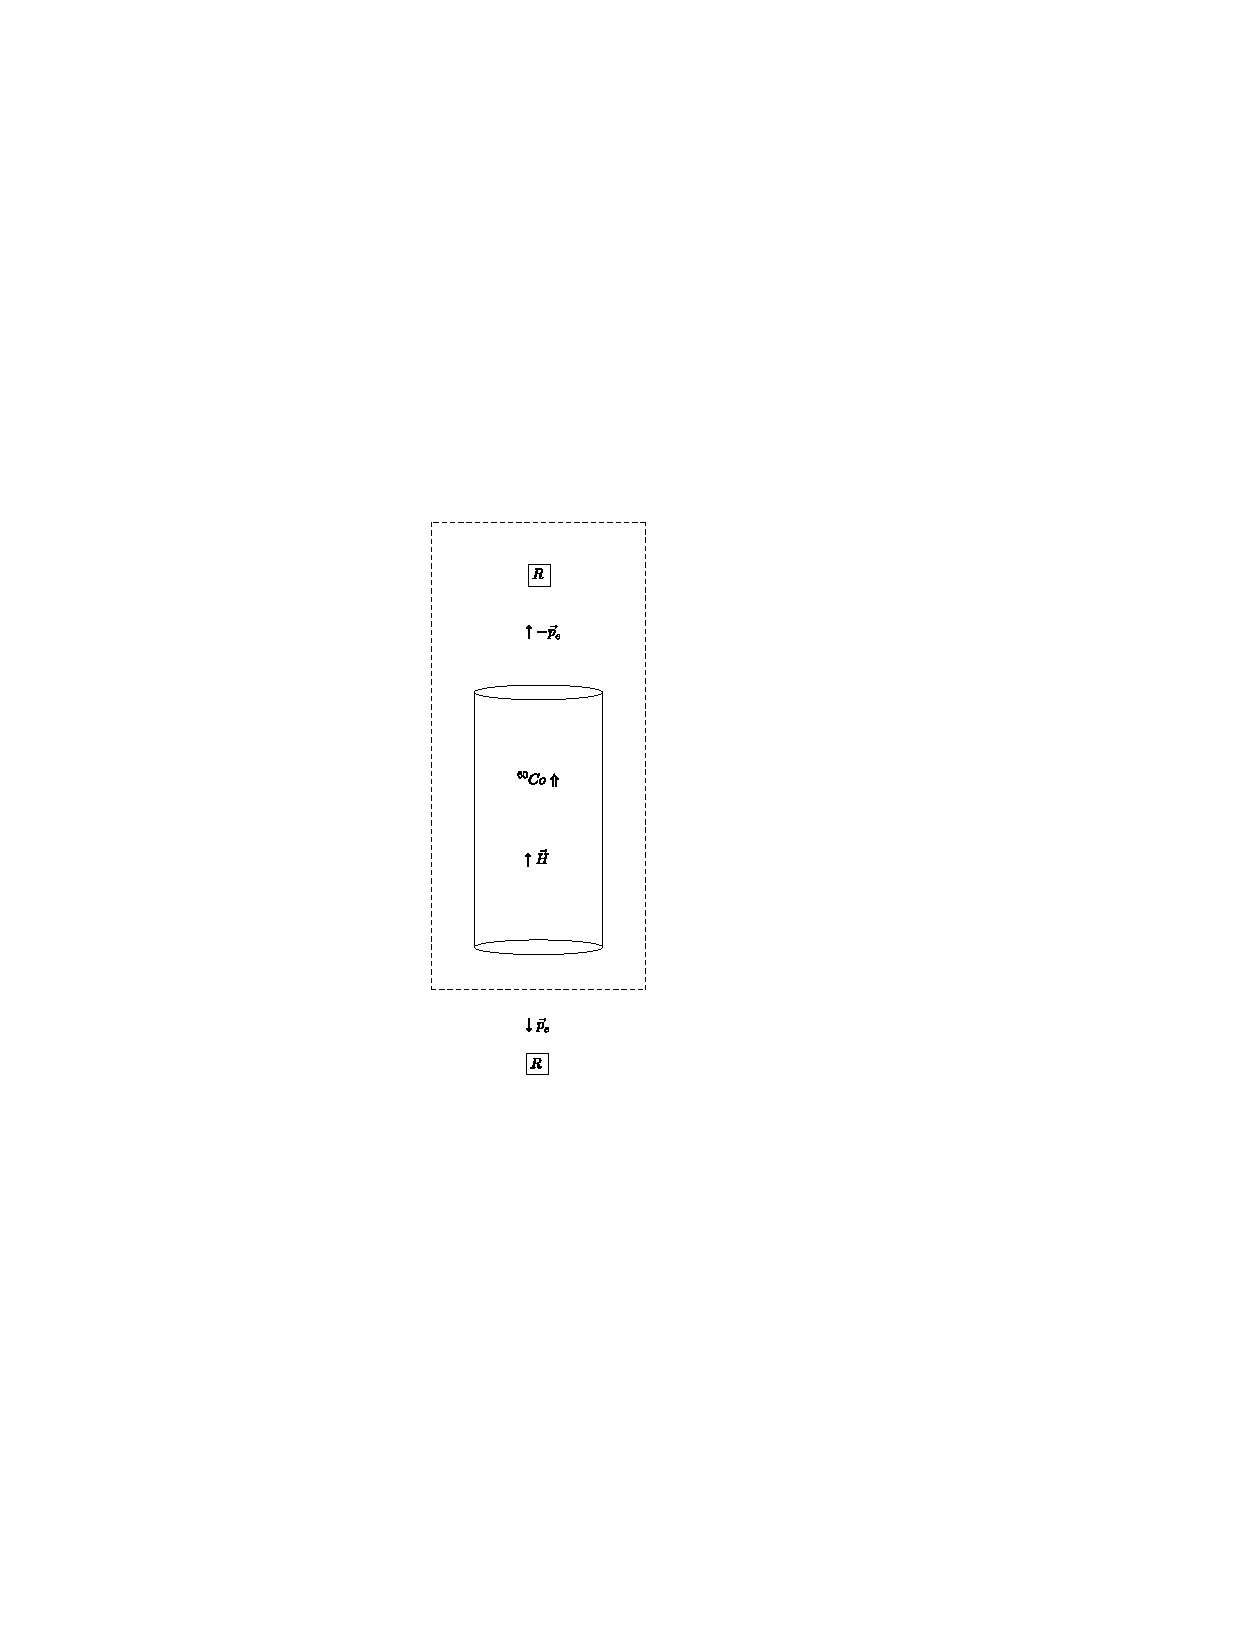
\includegraphics{img/dis_pboh1}
\end{figure}
Gli eventi osservati dall'osservatore di sopra saranno quelli spazialmente
riflessi dagli eventi osservati dall'osservatore di sotto. Questo perchè $p$ 
cambia segno,
mentre $H$ e lo spin no. In questo ragionamento abbiamo assunto che i nuclei di 
$\text{Co}^{60}$ sono a riposo in mdo da essere invarianti per inversione 
spaziale.
Quindi se nel processo fosse rispettata la simmetria per inversione spaziale i 
due rivelatori dovrebbero contare lo stesso numero di elettroni $\beta$ per 
unità di tempo.

Conteggi differenti implicherebbero una violazione della simmetria per 
inversione spaziale. Per effettuare le misure si utilizzò un solo rivelatore 
invertendo il senso della
corrente nel solenoide (vedi \autoref{dis_testo}). L'esperimento rivelò che 
gli elettroni venivano emessi in numero maggiore nella direzione opposta allo 
spin nucleare.
Si trovò che il fascio di elettroni emessi aveva una distribuzione angolare 
del tipo:
\[
I(\theta)=I_0(1-\frac{v}{c}\cos\theta)
\]
dove $\theta$ è l'angolo fra la direzione di emissione e lo spin nucleare.
Se fosse stata mantenuta la simmetria per inversione spaziale la dipendenza 
doveva essere del tipo $\cos^{2n}\theta$, in modo da avere simmetria attorno al 
piano azimutale
(vedi \autoref{dis_testo2}).
\begin{figure}[!hbt]
\centering
\caption{Seconda figura del testo originale.}
\label{dis_testo2}
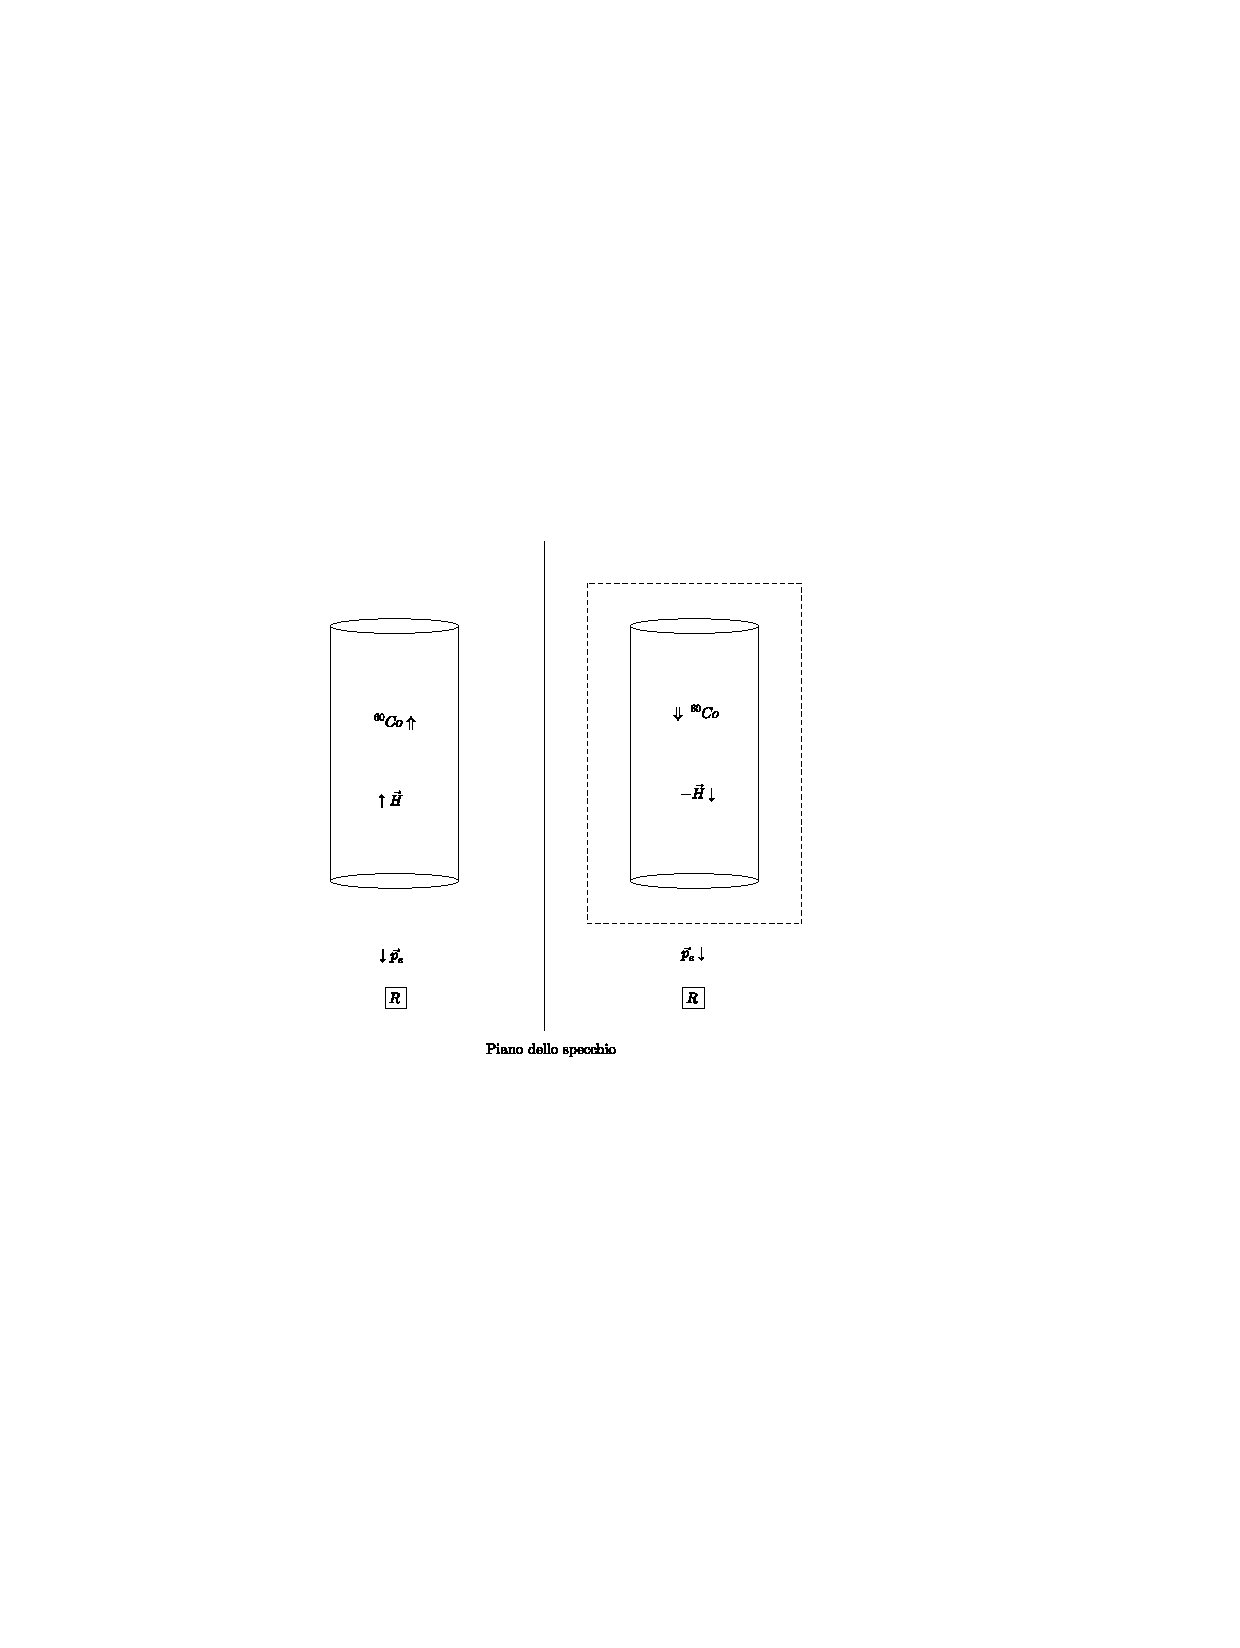
\includegraphics{img/dis_pboh2}
\end{figure}
L'importanza di questo esperimento è proprio la scoperta della violazione del 
principio di invarianza per inversione spaziale. Prima si credeva che il 
risultato di un esperimento
dovesse essere lo stesso se si usa un sistema o quello speculare.

Analizziamo\marginnote{6-3-1998} ora più in dettaglio questo esperimento e 
come è stato ricavato il risultato $\langle 
H\rangle_{e_{\beta}^-}=-\frac{v}{c}$.
Nella reazione
\[
\text{Co}^{60}\rightarrow \text{Ni}^{60}+e^-+\bar{\nu}
\]
lo spin nucleare diminuisce di un'unità pur rimanendo parallelo ad 
$\mathcal{H}$. La coppia elettrone-antineutrino ha momento angolare nullo 
rispetto al nucleo.
Per la conservazione del momento angolare totale l'elettrone e l'antineutrino 
devono avere spin $1/2$, orientato sempre nella stessa direzione:
\[
\Uparrow_{\text{Co}^{60}}\quad\Uparrow_{\text{Ni}^{60}}\quad\Uparrow_{1/2}\quad\
Uparrow_{1/2}
\]
Quindi un elettrone emesso longitudinalmente alla direzione dello spin avrà 
una polarizzazione longitudinale, quindi sarà in un autostato dell'elicità.
Per un angolo di emissione $\theta=0$ l'autovalore dell'elicità è $+1$, per 
$\theta=\pi$ l'autovalore dell'elicità è $-1$.
Indichiamo con $I_+$ e $I_-$ le intensità dei fasci di elettroni con 
$\theta=0$ e $\theta=\pi$. Il valore medio dell'elicità per un singolo 
elettrone sarà:
\[
\frac{(+1)I_++(-1)I_-}{I_++I_-}
\]
Abbiamo già detto che il risultato sperimentale per l'intensità è:
\begin{align*}
&I(\theta)=I_0(1-\frac{v}{c}\cos\theta)\\
&I_+=I(0)=I_0(1-\frac{v}{c})\\
&I_-=I(\pi)=I_0(1+\frac{v}{c})
\end{align*}
Quindi il valore medio di elicità risulta essere:
\[
\frac{(+1)I_+(-1)I_-}{I_++I_-}=-\frac{v}{c}
\]
\begin{itemize}
 \item Inversione spaziale = inversione di tutti e tre gli assi.
 \item Inversione speculare = inversione di un solo asse.
\end{itemize}
Queste due operazioni differiscono solo per una rotazione di $\pi$\footnote{\`E
presente nel testo una riga, purtroppo tagliata nella fotocopia, che risulta
illeggibile. (Ovviamente il professore vi chiederà quella)}.

Il sistema risulta simmetrico per inversione spaziale solo perché i nuclei di 
cobalto sono fermi, se così non fosse non si avrebbe questa simmetria iniziale 
e quindi non
ci si stupirebbe di riscontrare una asimmetria nei risultati.
\chapter{Teoria di Fermi}

Nel 1934 Fermi formulò una teoria fenomenologica del decadimento $\beta$ in 
accordo con i risultati sperimentali. Questo lavoro inaugurò la fisica delle 
particelle nucleari.
Questa teoria non prevedeva la violazione della simmetria speculare, ma lo 
schema di questa teoria rimane valido ancora oggi. Uno dei risultati di questa 
teoria è la spiegazione
degli spettri $\beta$. Sia $N_e$ il numero di elettroni emessi in un certo 
intervallo di tempo con un'energia cinetica compresa fra 
$[0,T_{\text{e,max}}]$, la distribuzione
di energia è data dalla funzione
\[
f(T_e)=\frac{dN_e}{dT_e}=\text{funzione di distribuzione}
\]
dove $dN_e$ è il numero di elettroni emessi con energia cinetica compresa 
nell'intervallo $[T_e,T_e+dT_e]$. Ovviamente deve essere:
\[
N_e=\int_0^{T_{\text{e,max}}}\frac{dN_e}{dT_e}dT_e
\]
Un altro importante risultato è la relazione fra $T_{\text{e,max}}$ e la vita 
media del nucleo che decade. Sulla base di questa teoria si possono enunciare 
alcune regole di selezione
che permettono una classificazione dei diversi decadimenti $\beta$ e la 
spiegazione del perché alcuni decadimenti sono meno favoriti di altri.

Il punto di partenza della teoria è la constatazione che l'interazione che 
determina il decadimento $\beta$ deve essere molto più piccola di quella 
elettromagnetica.

Consideriamo un nucleo a riposo di massa $M$ che decade in un nucleo di massa 
$M'$. Si ha che:
\begin{align*}
&Mc^2=M'c^2+Q\\
&Q=Mc^2-M'c^2=\text{Energia disponibile per la transizione}
\end{align*}
Questo parametro caratterizza la transizione e rappresenta tutta l'energia 
interna che il nucleo iniziale perde. L'energia di decadimento $E_d$ è la sola 
energia cinetica
che si genera nella transizione, infatti per definizione si ha:
\[
E_d=Mc^2-M'c^2-\sum_i m_ic^2
\]
quindi questa non caratterizza il decadimento come $Q$ perché dipende anche 
dalle masse delle altre particelle prodotte. Sperimentalmente si ha che a 
parità di $Q$ un nucleo che decade
per emissione $\beta$ ha vita media molto più lunga di quella di un nucleo che 
decade per emissione $\gamma$ ($Q\simeq1\si{\mega\electronvolt}$, 
$\tau_{\gamma}\simeq10^{-15}\si{\second}$,
$\tau_{\beta}\simeq10\text{min}$).
Questo fatto significa che $\lambda_{\beta}\ll\lambda_{\gamma}$, quindi la 
probabilità di decadimento è più piccola per un decadimento $\beta$ rispetto 
a quello $\gamma$.
Un altro fatto sperimentale è che:
\[
\tau_{\gamma}\gg 
T\equiv\frac{\hbar}{E}\simeq10^{-27}\si{\second}\quad(E\simeq100\,
\si{\giga\electronvolt})
\]
dove $T\cdot2\pi$ è il periodo caratteristico di oscillazione della funzione 
d'onda nucleare ($e^{-\frac{i}{\hbar}Et}$). Quindi nell'emissione $\gamma$ 
prima di decadere il nucleo
si trova in uno stato imperturbato il cui livello energetico coincide con il 
livello di energia $E$ a meno del parametro 
$\Gamma=\frac{\hbar}{\tau_{\gamma}}<<E$. Quindi l'intensità
dell'interazione $\beta$ è molto più piccola di quella $\gamma$. Da questo 
nasce il nome di \textit{interazione debole} per l'interazione responsabile del 
decadimento $\beta$.
L'hamiltoniana corrispondente risulterà molto più piccola di quella nucleare. 
Quindi possiamo usare la teoria delle perturbazioni fermandoci al primo ordine.
Sia $\mathcal{H}$ l'hamiltoniana totale del nucleo che decade. Si può scrivere 
nella rappresentazione di Schr\"{o}dinger:
\[
\mathcal{H}=\mathcal{H}_0+\mathcal{H}_{\text{int}}
\]
$\mathcal{H}_{\text{int}}$ non dipende dal tempo in quanto il sistema in esame 
è un sistema chiuso. Se passiamo dalla rappresentazione di interazione invece 
si ha:
\[
\mathcal{H}_I(t)=\mathcal{H}_0+\mathcal{H}_{\text{Iint}}(t)
\]
Lavoreremo sempre in questa rappresentazione, quindi in seguito sarà omesso il 
pedice $I$.

Possiamo assumere che il nucleo si trovi inizialmente nello stato $|i\rangle$, 
che sia autostato di $\mathcal{H}_0$ con autovalore $E_i$. Questa assunzione è 
esatta solo se l'istante iniziale
è $t=-\infty$, nella realtà non è così, ma dato che il nucleo ha una vita 
estremamente lunga questa è una buona approssimazione. Indichiamo con 
$|t\rangle$ lo stato del sistema
all'istante $t$. Si può scrivere:
\[
i\hbar\frac{d}{dt}|t\rangle=\mathcal{H}_{\text{int}}(t)|t\rangle
\]
con la condizione iniziale
\[
|t=0\rangle=|i\rangle
\]
Supponiamo \marginnote{9-3-1998} che i possibili stati finali abbiano uno 
spettro discreto. Questi stati finali sono autostati di $\mathcal{H}_0$. Si 
può scrivere:
\[
|t\rangle=\sum_fc_f(t)|f\rangle=\sum_{f\neq i}c_f(t)|f\rangle+c_{f= 
i}|f=i\rangle
\]
dove i coefficienti $c_f(t)$ sono definiti come:
\[
c_f(t)=\langle f|t\rangle
\]
Il modulo quadro di $c_f(t)$ dà la probabilità che all'istante $t$ il sistema 
si trovi nello stato $f$. Per la condizione iniziale deve essere:
\[
|c_{f\neq i}(0)|^2=0\quad |c_{f=i}|^2=1
\]
Per questo motivo le quantità $|c_f|^2(f\neq i)$ si dicono 
\textit{probabilità di transizione}. Lo stato finale può non avere energia 
uguale a quella iniziale.
Questo perché l'energia del sistema fra $t=0$ e $t$ è soggetta alla relazione:
\[
\Delta E_i=\frac{\hbar}{t}
\]
Quindi le transizioni possono avvenire fra stati la cui energia è compresa 
nell'intervallo $[E_i-\frac{\Delta E_i}{2},E_i+\frac{\Delta E_i}{2}]$.
Deve però essere sempre verificato che:
\[
\langle\mathcal{H}\rangle=\langle t|\mathcal{H}(t)|t\rangle=E_i
\]
La quantità $\frac{\Delta E_i}{2}$ non può superare il valore di $E_i$, 
quindi:
\[
\Delta E_i\leq2E_i
\]
Le probabilità di transizione risulteranno molto minori di $1$, quando la 
pertirbazione $\mathcal{H}_{\text{int}}(t)$ è molto piccola, anche per $t$ 
molto grandi, cioé:
\[
|C_{f\neq i}|^2<<1\quad(t>>\frac{\hbar}{E_i})
\]
Ma in queste condizioni (essendo $t=\frac{\hbar}{\Delta E_i}$) deve essere 
$\Delta E_i<<E_i$. Avvengono quindi transizioni a stati finali la cui energia 
è $E_f\simeq E_i$.
La condizione $E_f=E_i$ è esatta se $\mathcal{H}_{\text{int}}$ è un 
infinitesimo. Infatti in questo caso una transizione  ad uno stato può 
avvenire solo per $t$ tendente ad infinito:
\[
\lim_{t\rightarrow+\infty}\Delta E_i=\lim_{t\rightarrow+\infty}\frac{\hbar}{t}=0
\]
Possiamo assumere per l'hamiltoniana di interazione $\beta$ che questa sia un 
infinitesimo rispetto ad $\mathcal{H}_0$, e quindi la transizione può avvenire 
solo a $t\rightarrow+\infty$.
In queste ipotesi si hanno transizioni fra stati che hanno energia finale 
uguale a quella iniziale.

Passiamo ora ad una trattazione più rigorosa considerando tutti i possibili 
stati finali. Per un lungo intervallo a partire da $t=0$ si ha:
\[
|c_{f\neq i}(t)|^2\simeq |c_{f\neq i}(0)|^2=0
\]
Se ci si ferma al primo ordine nella teoria delle perturbazioni si può 
scrivere:
\[
|c_{f\neq 
i}(t)|^2=2|\mathcal{H}_{\text{if}}|^2\frac{1-\cos(\omega_{\text{if}}t)}{(E_f-E_i
)^2}
\]
dove si è posto:
\begin{align*}
&\omega_{\text{if}}=\frac{E_f-E_i}{\hbar}\\
&|\mathcal{H}_{\text{if}}|^2\equiv\langle 
f|\mathcal{H}_{\text{int}}|i\rangle\propto e^{i\omega_{\text{if}}t}\quad 
(|f\rangle\neq|i\rangle)\\
&|\mathcal{H}_{\text{if}}|^2=\text{costante}
\end{align*}
(questo si può dedurre considerando che i prodotti scalari non dipendono dalla 
rappresentazione).
\[
\frac{d}{dt}|c_{f\neq 
i}(t)|^2=\frac{2}{\hbar}|\mathcal{H}_{\text{if}}|^2\frac{\sin(\omega_{\text{if}}
t)}{E_f-E_i}
\]
Attenzione!\footnote{Nel testo è presente, scritta minuscola, la formula
  $\frac{d}{dt}|c_{f\neq i}|^2=
2|\mathcal{H}_{\text{if}}|^2\,\frac{\sin(\omega_{\text{if}}t)}{(E_f-E_i)^2
}\omega_{\text{if}}$. Questa è la stessa formula a meno delle semplificazioni.}

Se approssimiamo $\mathcal{H}_{\text{int}}$ ad un infinitesimo, 
$\mathcal{H}_{\text{if}}$ lo sarà pure.
In questo caso dobbiamo considerare il limite:
\begin{align*}
&\lim_{t\rightarrow+\infty}\bigl[\frac{d}{dt}|c_{f\neq 
i}(t)|^2\bigr]=
\frac{2}{\hbar}|\mathcal{H}_{\text{if}}|^2\lim_{t\rightarrow+\infty}
\frac{\sin(\omega_{\text{if}}t)}{E_f-E_i}\\
&\lim_{t\rightarrow+\infty}\frac{\sin(\omega_{\text{if}}t)}{E_f-E_i}=
\frac{\pi}{\hbar}\lim_{t\rightarrow+\infty}\frac{\sin(\omega_{\text{if}}t)}{\pi
\omega_{\text{if}}}=\frac{\pi}{\hbar}\delta(\omega_{\text{if}})\\
&\delta(\omega_{\text{if}})=\lim_{t\rightarrow+\infty}
\frac{\sin(\omega_{\text{if}}t)}{\pi\omega_{\text{if}}}=\hbar\lim_{\frac{t}{\hbar}
\rightarrow+\infty}\frac{\sin[(E_f-E_i)t/\hbar]}{\pi(E_f-E_i)}=\hbar\delta(E_f-E_i)
\end{align*}
L'uguaglianza fra la funzione $\delta$ ed il limite è un'uguaglianza fra 
funzionali e non fra funzioni.
Quindi\marginnote{11-3-1998} nel limiti di un'hamiltoniana di interazione 
infinitesima saranno accessibili solo stati finali con $E_f=E_i$.
\[
W_{\text{if}}=\lim_{t\rightarrow+\infty}[\frac{d}{dt}|c_{f\neq 
i}(t)|^2]=\frac{2\pi}{\hbar}|\mathcal{H}_{\text{if}}|^2\delta(E_f-E_i)=\text{cos
tante}
\]
Questa è la probablità di transizione  da $i$ ad $f$ nell'unità di tempo. Si 
può definire la probabilità totale di transizione nell'unità di tempo come:
\[
W=\sum_{f\neq i}W_{\text{if}}=\frac{2\pi}{\hbar}\sum_{f\neq 
i}|\mathcal{H}_{\text{if}}|^2\delta(E_f-E_i)=\text{Probabilità totle di 
transizione nell'unità di tempo.}
\]
Di fatto si ha che $W_{\text{if}}=0$ se $E_f\neq E_i$, quindi gli unici 
contributi provengono da stati $f$ con $E_f=E_i$.

Tutti i risultati sono stati trovati lavorando al primo ordine. Se consideriamo 
anche ordini sccessivi di approssimazione allora il procedimento al limite 
porta sempre ad una $W$ costante.
Quindi si può scrivere la probabilità totale mediante la formula:
\[
W=\frac{2\pi}{\hbar}\sum_{f\neq i}|T_{\text{if}}|^2\delta(E_f-E_i)
\]
dove $T_{\text{if}}$ ha le dimensioni di energia. Questi coefficienti si dicono 
elementi di matrice relativi alla transizione dallo stato $i$ allo stato $f$.

Fino ad ora abbiamo lavorato sull'ipotesi di spettro discreto. Di solito si 
hanno spettri continui, sappiamo che questi però possono essere approssimati 
con spettri quasi continui.
Per fare questa approssmazione si deve introdurre la densità di stati finali 
come:
\[
\rho_f(E_f)=\frac{dN}{dE_f}|_{E_f}\quad\text{$dN=$ numero di stati finali con 
energia compresa nell'intervallo $[E_f,E_f+dE_f]$.}
\]
E si deve fare la sostituzione:
\[
\sum_f\rightarrow\int N=\int\rho_f(E_f)dE_f
\]
Quindi la probabilità totale nell'unità di tempo $W$ diventa:
\[
W=\frac{2\pi}{\hbar}\int|\mathcal{H}_{\text{if}}|^2\delta(E_i-E_f)\rho_f(E_f)dE_
f=\frac{2\pi}{\hbar}|T_{\text{if}}|^2\rho_f(E_i)
\]
dove in prima approssimazione si può scrivere:
\[
W=\frac{2\pi}{\hbar}|\mathcal{H}_{\text{if}}|^2\rho_f(E_i)\quad\text{\textsc{Reg
ola d'oro
di Fermi}}
\]
Secondo questa formula $W$ è data dal prodotto di due fattori: uno di natura 
dinamica ($|\mathcal{H}_{\text{if}}|^2$), mentre l'altro è non dinamico ed è 
la densità
di stati finali con $E_f=E_i$: $\rho_f(E_i)=\frac{dN}{dE_f}|_{E_f=E_i}$.

Se si vuole passare al caso continuo dal caso quasi continuo si deve fare il 
limite per $V\rightarrow+\infty$ dove $V$ è il volume della scatola.

Se vogliamo applicare la regola d'oro al decadimento $\beta^-$ si deve 
specificare l'elemento di matrice $T_{\text{if}}$, che al primo ordine è 
$\mathcal{H}_{\text{if}}$.
L'hamiltoniana di interazione rappresenta una perturbazione piccola in 
confronto all'hamiltoniana nucleare, quindi:
\[
\tau_{\beta}>>\tau_{\gamma}>>T=\frac{\hbar}{E}
\]
Si può quindi assumere $\tau_{beta}=\infty$. Nell'intervallo di tempo fra $0$ 
e $\tau_{\beta}$ la funzione d'onda quasi stazionaria si può scrivere come:
\[
\begin{split}
\psi 
&=\psi(0)e^{-\frac{i}{\hbar}Et}e^{-\frac{t}{2\tau_{\beta}}}=\psi(0)e^{-i\frac{t}
{T}-\frac{t}{2\tau_{\beta}}}\simeq\\
&\simeq\psi(0)e^{-i\frac{t}{T}}=\psi(0)e^{-\frac{i}{\hbar}Et}\quad(0\leq 
t<\tau_{\beta})\quad(\text{Questo è uno stato stazionario.})
\end{split}
\]
Quindi in questa approssimazione il nucleo si trova in uno stato non perturbato 
per tutto il tempo di vita media. Per questo il decadimento $\beta$ si può 
considerare
come un processo dinamico di durata istantanea. Secondo la teoria della 
relatività tutte le interazioni hanno una velocità di propagazione finita. 
Quindi il decadimento $\beta$
può avvenire solo in una regione puntiforme del nucleo (la sua durata è 
istantanea).
Per questo il decadimento $\beta$ coinvolge un solo nucleone ed è lecito 
scrivere:
\[
n\rightarrow p^++e^-+\bar{\nu}
\]
Quindi $\mathcal{H}_{\text{int}}$ di un nucleo soggetto ad un decadimento 
$\beta^-$ è identica a quella di un neutrone che decade in un protone.
\breaknote

In\marginnote{13-3-1998} base alla teoria di Dirac un fermione con 
quadriimpulso $p^{\mu}$ che viene creato in un punto spaziotemporale è 
equivalente alla distruzione di
un fermione con quadrimpulso opposto nello stesso punto spaziotemporale. Quindi 
se a $\bar{\nu}$ che viene creato sostituiamo un $\nu$ distrutto possiamo 
considerare
il processo di diffusione:
\[
n+\nu\rightarrow p^++e^-\quad(\Leftrightarrow n\rightarrow p^++e^-+\bar{\nu} 
\text{ decadimento $\beta^-$})
\]
che è caratterizzato dalla stessa $\mathcal{H}_{\text{int}}$ del processo di 
sopra. Il decadmento $\beta^-$ di un neutrone equivale dal punto di vista 
dinamico al processo rappresentato nel
diagramma in \autoref{fig:dia_fey}.
\begin{wrapfigure}{l}{5.5cm}
\centering
\caption{}
\label{fig:dia_fey}
\begin{tikzpicture}[scale=1, >=triangle 45]
  \draw [->] (-2,-2) -- (-1,-1) node [right=10pt] {$n$};
  \draw [->] (-1,-1) -- (1,1) node [right=10pt] {$e^-$};
  \draw (1,1) -- (2,2);
  \draw [->] (2,-2) -- (1,-1) node [right=10pt] {$\nu$};
  \draw [->] (1,-1) -- (-1,1) node [left=10pt] {$p^+$};
  \draw (-1,1) -- (-2,2);
  \filldraw (0,0) circle (1pt);
  \begin{scope}[>=stealth]
    \draw [<-] (.2,0) -- (2,0) node [right=5pt] {vertice};
  \end{scope}
\end{tikzpicture}
\end{wrapfigure}

In questo processo sono coinvolte quattro particelle (due entranti e due 
uscenti). Queste interagiscono solo nel punto di incontro che si dice 
\textit{vertice del diagramma}.
Un'interazione caratterizzata da un solo vertice si dice \textit{interazione di 
contatto} oppure \textit{processo del primo ordine}.

In un processo di diffusione di due particelle  il potenziale di interazione 
dipenderà solo da $|\vec{r_1}-\vec{r_2}|$. Supponiamo che le due particelle 
siano descritte da funzioni d'onda
scalari, siano queste $\psi_1(\vec{r_1})$, $\psi_2(\vec{r_2})$. Per definizione 
si ha:
\[
\mathcal{H}_{\text{if}}=\langle f|\mathcal{H}_{\text{int}}|i\rangle=\int 
\psi^*_{1f}(\vec{r_1})\psi^*_{2f}(\vec{r_2})V(|\vec{r_1}-\vec{r_2}|)\psi_{1i}
(\vec{r_1})\psi_{2i}(\vec{r_2})d^3r_1d^3r_2
\]
Questa formula vale anche per una diffusione anelastica, cioé anche se le 
particelle subiscono trasformazioni interne. Nel caso che stiamo considerando 
si ha un \textit{potenziale di contatto},
quindi il potenziale si può scrivere come:
\[
V(|\vec{r_1}-\vec{r_2}|)=g\delta^3(|\vec{r_1}-\vec{r_2}|)
\]
dove $g$ è una costante da determinare sperimentalmente. Con questa scelta per 
$V$ possiamo calcolare l'elemento di matrice:
\[
\mathcal{H}_{\text{if}}=g\int 
\psi^*_{1f}(\vec{r})\psi^*_{2f}(\vec{r})\psi_{1i}(\vec{r})\psi_{2i}(\vec{r})d^3\
vec{r}
\]
Questa in realtà non è esatta in quanto le particelle hanno uno spin $1/2$ e 
quindi le funzioni d'onda non sono scalari ma spinori. Per il momento comunque 
trascureremo questo fatto. Poniamo:
\[
\psi_{1i}=\psi_n;\quad\psi_{2i}=\psi_{\nu};\quad\psi_{1f}=\psi_p;\quad\psi_{2f}=
\psi_e
\]
Si ottiene dunque (V = volume nucleare):
\[
\mathcal{H}_{\text{if}}^{(\beta)}=
g\int_V\psi^*_p(\vec{r})\psi^*_e(\vec{r})\psi_n(\vec{r})\psi_{\nu}(\vec{r})d^3\vec{r}
\]
questo integrale è esteso al volume nucleare e $\vec{r}$ rappresenta la 
posizione del neutrone rispetto al centro del nucleo. La costante $g$ si dice 
\textit{costante di accoppiamento di Fermi}.
Questa ha le dimensioni di energia per volume. Le due funzioni d'onda 
$\psi^*_e$ e $\psi_{\nu}$ si possono scrivere nella forma stazionaria:
\begin{align*}
&\psi_e^*(\vec{r})=\frac{1}{\Omega^{1/2}}e^{-i\vec{k_e}\cdot\vec{r}}\\
&\psi_{\nu}(\vec{r})=\frac{1}{\Omega^{1/2}}e^{i\vec{k_{\nu}}\cdot\vec{r}}
\end{align*}
con
\begin{align*}
&\vec{k_e}=\frac{1}{\hbar}\vec{p}\\
&\vec{k}_{\nu}=-\vec{k}_{\bar{\nu}}
\end{align*}
$\Omega$ è il volume dove è racchiuso il sistema\footnote{Quello relativo 
all'approssimazione al caso quasi continuo. .}.
Con questa scelta si trascurano le interazioni tra il neutrino o l'elettrone 
con il nucleo\footnote{Ad esempio si trascurano le forze elettromagnetiche. }.
Di solito gli impulsi di $e^-$ e $\nu$ sono di un ordine di grandezza tale che:
\[ 
\text{\textcrlambda}=\frac{\lambda}{2\pi}=\frac{1}{k}=\frac{\hbar}{p}\gtrsim2
\cdot10^{-11}\,\si{\centi\meter}
\]
Quindi \textcrlambda è molto grande in confronto alle dmensioni nucleari. Se 
poniamo:
\begin{align*}
&e^{-i\vec{k_e}\cdot\vec{r}}=1-i\vec{k_e}\cdot\vec{r}+\dots\\
&e^{i\vec{k_{\nu}}\cdot\vec{r}}=1+i\vec{k_{\nu}}\cdot\vec{r}+\dots
\end{align*}
si avrà che per ogni punto $\vec{r}$ interno al nucleo:
\[
\vec{k_e}\cdot\vec{r}<<1;\quad\vec{k_{\nu}}\cdot\vec{r}<<1
\]
Ci si può dunque fermare ai termini di ordine zero nello sviluppo in serie:
\[
\psi_e^*(\vec{r})\psi_{\nu}(\vec{r})\simeq\psi_e^*(0)\psi_{\nu}(0)=\frac{1}{\Omega}
\]
questa approssimazione è possibile a patto che l'elemento di matrice che si 
ottiene non risulti nullo. Ogni volta che questo è verificato si può scrivere:
\begin{align*}
&\mathcal{H}_{\text{if}}^{(\beta)}\simeq 
g\int\psi_p^*(\vec{r})\psi_n(\vec{r})\psi_e^*(0)\psi_{\nu}(0)d^3\vec{r}\neq0\\
&\mathcal{H}_{\text{if}}^{(\beta)}\simeq\mathcal{H}_{\text{if}}^{(0)}\equiv 
g\frac{M_{\text{if}}}{\Omega}\,\text{dove}\quad 
M_{\text{if}}=\int\psi_p^*(\vec{r})\psi_n(\vec{r})d^3\vec{r}
\end{align*}
dove $M_{\text{if}}$ è un numero puro. Questa approssimazione corrisponde 
all'approssimazione di monopolo, e il nucleo non è altro che un punto rispetto 
a $\lambda_e$ e $\lambda_{\nu}$.
Quindi l'elettrone e l'antineutrino non possono avere un $L$ rispetto al nucleo
in quanto sono stati emessi da una sorgente puntiforme. Quindi il sistema 
$e^-+\bar{\nu}$ ha due possibilità
per il momnto angolare totale: $0$ (singoletto), $1$ (tripletto). Nel primo caso
si parla di \textit{transizione di Fermi}, nel secondo caso si dice 
\textit{transizione di Gamow Teller}.
Nel primo caso vale la regola di selezione di Fermi secondo cui le transizioni 
permesse sono solo quelle per cui:
\[
  \Delta j=j_f-j_i=0\quad\text{\textsc{Regola di Fermi}}
\]
Nel secondo caso vale la regola di selezione di Gamow-Teller secondo cui è
proibita ogni transizione con \#\#\#\footnote{Cosa stranissima: lo spazio è
bianco anche nel testo, ed è presente una freccina
con un punto interrogativo? Era finito l'inchiostro? Sbobinatura non chiara?
Prossimamente a Voyager! NdT.}, mentre sono permesse solo transizioni per cui:
\[
 j_{\text{fin}}-1\leq j_{\text{in}}\leq j_{\text{fin}}+1
\]
che implica
\[
\begin{sistema}
\Delta j=\pm1\\
\Delta j=0\;(i\neq0)
\end{sistema}\qquad\text{\textsc{Regola di selezione di Gamow-Teller}}
\]
In particolare la transizione $\beta$ del $\text{Co}^{60}$ è una transizione di
Gamow-Teller ``permessa''. Queste regole di selezione valgono solo nelle 
approssimazioni considerate
perché sono state dedotte dall'ipotesi che fosse nullo il momento orbitale del
sistema $e^-+\bar{\nu}$. Nella risoluzione esatta del problema si trovano delle 
transizioni $\beta$ che
non rientrano fra le regole di selezione enunciate, queste transizioni però 
sono
meno favorite in quanto i corrispondenti elementi di matrice sono di ordine più
piccolo rispetto
agli elementi di matrice della transizione permessa.

Abbiamo\marginnote{16-3-1998} visto che sotto certe ipotesi si ha: 
$\mathcal{H}_{\text{if}}=g\frac{M_{\text{if}}}{\Omega}$.
Abbiamo anche ricavato le regole di selezione e commentato la loro validità. Se
consideriamo solo le transizioni permesse, la regola d'oro di Fermi assume la
forma:
\[
W=\frac{2\pi}{\hbar}|\mathcal{H}_{\text{if}}(0)|^2\rho_f(E_i)=\frac{2\pi}{\hbar
\Omega^2}g^2|M_{\text{if}}|^2\rho_f(E_i)
\]
L'elemento di matrice $\mathcal{H}_{\text{if}}$ che compare in $W$ non dipende
dai momenti delle particelle interagenti, quindi questa può essere interpretata
come probabilità di transizione
complessiva nell'unità di tempo per tutti i possibili valori dei momenti. 
Questa
interpretazione è corretta se $\rho_f(E_i)$ è la densità complessiva di stati
finali con energia $E_i$.
Quindi $W$ è la probabilità di decadimento $\beta$ nell'unità di tempo, 
dunque deve essere:
\[
W=\lambda_{\beta}
\]
Se poniamo per l'energia finale $E_f$:
\[
E_f=M'c^2+Q
\]
dove $M'$ è la massa del nucleo prodotto e $Q$ l'energia disponibile. Si avrà:
\[
dE_f=dQ\Rightarrow\rho_f=\frac{dN}{dE_f}|_{E_f=E_i}=\frac{dN}{dQ}|_{Q=E_i-M'c^2}
\]
dove $dN$ è il numero totale di stati finali con energia compresa fra $E_i$ e
$E_i+dQ$. Per l'energia $Q$ si avrà:
\[
Q=E_e+E_{\bar{\nu}}+T_R
\]
dove $E_e$ è l'enrgia totale dell'elettrone, $E_{\bar{\nu}}$ l'energia totale
dell'antineutrino, $T_R$ l'energia di rinculo del nucleo.
Ma dal momento che $T_R<<E_e,E_{\bar{\nu}}$ si ha:
\[
Q=E_e+E_{\bar{\nu}}=(m_e^2c^4+c^2p_e^2)^{1/2}+cp_{\bar{\nu}}
\]
La forma dello spettro\footnote{Spettro $\beta=$ numero di elettroni con una
certa energia} $\beta$ si può ricavare direttamente dalla conoscenza della
funzione:
\[
\frac{dW}{dE_e}=\frac{dW}{dT_e}
\]
Il numero $M_{\text{if}}$ non dipende da $T_e$, allora la forma dello spettro
$\beta$ è determinata solo dalla conoscenza della funzione $\rho_f(E_i)$.
Dobbiamo calcolare la funzione:
\[
\frac{d\rho_f}{dT_e}=\frac{d^2N}{dT_edQ}
\]
in quanto:
\[
\frac{dW}{dT_e}\propto\frac{d\rho_f}{dT_e}
\]
Possiamo equivalentemente calcolare la funzione :
\[
\frac{d\rho_f}{dp_e}=\frac{d^2N}{dp_edQ}\quad\text{in 
quanto}\quad\frac{dW}{dp_e}\propto\frac{d\rho_f}{dp_e}
\]
Facciamo l'ipotesi che la scatola immaginaria in cui si suppone racchiuso il 
sistema sia un cubo di lato $L$ con gli spigoli paralleli agli assi $x,y,z$. Si 
potrebbe assumere che le
funzioni d'onda di $e$ e $\bar{\nu}$ si annullino sulle pareti della scatola, 
ma questo non può essere verificato in quanto sono funzioni complesse. La 
condizione meno restrittiva che si può
imporre è che le funzioni d'onda siano invarianti per traslazioni:
\[
x\rightarrow x+L\quad y\rightarrow y+L\quad z\rightarrow z+L
\]
quindi i vettori d'onda devono verificare la condizione:
\[
k_{\alpha}L=2\pi n_{\alpha}\quad(\alpha=x,y,z\;\;n_{\alpha}=0,\pm1,\pm2,\dots)
\]
Lo spettro continuo di $p_e$ e $p_{\bar{\nu}}$ si riduce in questo caso ad uno 
spettro discreto, dove i possibili valori per le componenti sono:
\[
p_{\alpha}=\hbar k_{\alpha}=\frac{2\pi\hbar}{L}n_{\alpha}\quad(\alpha=x,y,z)
\]
Quindi per un dato intervallo $\Delta p_{\alpha}=p_{\alpha}''-p_{\alpha}'>0$ il 
numero di valori che $p_{\alpha}$ può assumere in questo intervallo è:
\[
\Delta n_{\alpha}=n_{\alpha}''-n_{\alpha}'\Rightarrow\frac{\Delta 
n_{\alpha}}{\Delta p_{\alpha}}=\frac{L}{2\pi\hbar}=\text{costante}
\]
Questo rapporto coincide con il numero di autostati di $p_{\alpha}$ per 
intervallo unitario di $p_{\alpha}$. Per ciascuna particella emessa nel 
decadimento la densità di stati è data
dalla quantità:
\[
\frac{\Delta n_x}{\Delta p_x}\frac{\Delta n_y}{\Delta p_y}\frac{\Delta 
n_z}{\Delta 
p_z}=\frac{L^3}{(2\pi\hbar)^3}=\frac{\Omega}{(2\pi\hbar)^3}=\text{densità 
degli stati}
\]
Nell'approssimazione quasi continua il numero di stati di una particella in un 
volumetto $dp_xdp_ydp_z$ è:
\[
\frac{\Omega}{(2\pi\hbar)^3}dp_xdp_ydp_z=\frac{\Omega}{(2\pi\hbar)^3}p^2\sin\theta
dpd\theta d\phi\quad\text{(in coordinate polari nello spazio dei momenti)}
\]
Il corrispondente numero di stati nell'intervallo $[p,p+dp]$ si ottiene 
integrando su $\theta$ e $\phi$. Per l'elettrone si ottiene:
\[
dN_e=\frac{4\pi\Omega}{(2\pi\hbar)^3}p_e^2dp_e
\]
Per l'antineutrino si ottiene:
\[
dN_{\bar{\nu}}=\frac{4\pi\Omega}{(2\pi\hbar)^3}p^2_{\bar{\nu}}dp_{\bar{\nu}}
\]
Trattandosi di una disintegrazione a tre corpi $p_e$ e $p_{\bar{\nu}}$ possono 
considerarsi indipendenti una dall'altra. Quindi il numero totale di stati 
finali in cui l'elettrone ha la quantità
di moto compresa nell'intervallo $[p_e,p_e+dp_e]$ e l'antineutrino 
nell'intervallo $[p_{\bar{\nu}},p_{\bar{\nu}}+dp_{\bar{\nu}}]$ è:
\[
d^2N=dN_edN_{\bar{\nu}}=\frac{16\pi^2\Omega^2}{(2\pi\hbar)^6}p_e^2dp_ep_{\bar{
\nu}}^2dp_{\bar{\nu}}
\]
Considerato che:
\[
p_{\bar{\nu}}=\frac{Q-E_e}{c}\Rightarrow dp_{\bar{\nu}}=\frac{dQ}{c}
\]
In quanto per calcolare $dp_{\bar{\nu}}$ si deve tenere fisso $dp_e$. 
Sostituendo quest'espressione in quella per $dN^2$ si ottiene:
\begin{align*}
&d^2N=\frac{16\pi^2\Omega^2}{(2\pi\hbar)^6c^3}(Q-E_e)^2p_e^2dp_edQ\\
&\frac{d\rho_f}{dp_e}=\frac{d^2N}{dp_edQ}=\frac{16\pi^2\Omega^2}{(2\pi\hbar)^6c^
3}(Q-E_e)^2p_e^2\\
&\frac{dW}{dp_e}=\frac{2\pi}{\hbar}g^2|M_{\text{if}}|^2\frac{16\pi^2}{(2\pi\hbar
)^6c^3}(Q-E_e)^2p_e^2
\end{align*}
Come ci si doveva aspettare, in questa espressione non compare più il volume 
$\Omega$. Lo spettro $\beta$ così ottenuto rimane valido anche quando $\Omega$ 
è variabile
e quindi anche per $\Omega\rightarrow\infty$. La forma dello spettro $\beta$ 
che si ottiene è rappresentata in \autoref{fig:spettro_beta}.
\begin{figure}[!h]
  \centering
  \caption{Spettro $\beta$.}
  \label{fig:spettro_beta}
  \begin{tikzpicture}[line cap=round,line join=round,>=stealth,x=6.56433537135226cm,y=14.487115647952196cm]
  \draw[->,color=black] (-0.01,0) -- (1.36,0) node [below]
  {$p_e$};
  \foreach \x in {0,0.2,0.4,0.6,0.8,1,1.2}
  \draw[shift={(\x,0)},color=black] (0pt,2pt) -- (0pt,-2pt);
  \draw[->,color=black] (0,-0.01) -- (0,0.33) node [left] {$\frac{\text{d}W}{\text{d}p_e}$};
  \foreach \y in {0,0.1,0.2,0.3}
  \draw[shift={(0,\y)},color=black] (2pt,0pt) -- (-2pt,0pt);
  \clip(-0.01,-0.01) rectangle (1.48,0.35);
  \draw[smooth,samples=100,domain=0:1.35]
  plot(\x,{(\x)^2*sqrt(1.25^2+0.5^2)-(\x)^2*sqrt((\x)^2+0.5^2)});
  \fill [color=\MinorColor] (1.25,0) circle (1.5pt) node [above right]
  {$p_{e,\text{max}}$};
\end{tikzpicture}

\end{figure}
Dalla conoscenza della funzione $\frac{dW}{dp_e}$ si può ricavare il parametro 
$\lambda_{\beta}$, infatti:
\[
\lambda_{\beta}=W=\int_0^{P_{\text{e,max}}}\frac{dW}{dp_e}dp_e
\]
dove
\[
p_{\text{e,max}}=\frac{1}{c}\sqrt{E_{\text{e,max}}^2-m_e^2c^4}\quad\text{con}\;E
_{\text{e,max}}=Q
\]
quindi per $\lambda_{\beta}$ si ottiene:
\[
\lambda_{\beta}=\lambda_{\beta}(p_{\text{e,max}})=\frac{g^2|M_{\text{if}}|^2}{2\
pi^3c^3\hbar^7}\int_0^{p_{\text{e,max}}}[Q-(m_e^2c^4+c^2p_e^2)^{1/2}]^2p_e^2dp_e
\]
Questa espressione ci dà il legame fra $\lambda_{\beta}$ e $p_{\text{e,max}}$, 
o l'energia massima che l'eletrone può avere. Queste formule, con opportune 
correzioni di tipo
elettromagnetico, forniscono valori teorici molto vicini a quelli sperimentali 
per molte transizioni $\beta$ permesse, se però si pone:
\[
g=1,4\cdot10^{-49}\;\text{erg}\cdot\si{\centi\meter}^3\quad 
g\equiv\text{costante di accoppiamento di Fermi.}
\]

\chapter{Forze Nucleari}

Un \marginnote{18-03-1998}  \textit{nucleo atomico} è un aggregato di protoni 
e neutroni.

L'esistenza di nuclei stabili implica l'esistenza di forze attrattive, che sono
conseguenza  dell'energia di legame e del difetto di massa. Queste forze devono
vincere la repulsione elettromagnetica; il raggio caratteristico di questa fase
è $10^{-13} cm$, che si ricava dagli esperimenti sulla diffusione. Il modello a
goccia di liquido assume che la forza attrattiva sia indipendente dalla natura
del nucleone (sia questo un protone o un neutrone). Questa assunzione implicita
è confermata dal successo della formula per la massa che si ricava da questa
ipotesi, ma anche altri fatti sperimentali ne confermano la validità. Uno di
questi fatti si basa sui nuclei isobari speculari (si ottengono scambiando i
numeri di protoni e neutroni). La massa di questi nuclei è la stessa a meno del
termine relativo all'energia coulombiana. 

Consideriamo ad esempio due nuclei
\begin{align*}
	( Z_{1}& = Z \ ;  \quad N_{1} = Z+1 ) &  ( Z_{2}& = Z+1 \ ;  \quad 
N_{2} = Z) 
\end{align*}
una coppia di questo tipo presenta una differenza di massa 
\begin{equation*}
	 \Delta M = \Delta M_{c} 
\end{equation*}
dove $\Delta M_{c}$ è la differenza dovuta all'energia coulombiana.

\begin{equation}
\begin{split}
	\Delta M_{c} &= \dfrac{3}{5} \dfrac{e^2 (z_{2})^2}{c^2(r_{0})^2 
A^{1/3}} - \dfrac{3}{5} \dfrac{e^2 				
(z_{1})^2}{c^2(r_{0})^2 A^{1/3}} = \dfrac{3}{5} \dfrac{e^2}{c^2(r_{0})^2 
A^{1/3}} 				\bigl[ (z+1)^2-z^2 \bigr ] \\
			&= \dfrac{3}{5} \dfrac{e^2}{c^2(r_{0})^2 A^{1/3}} (2z+1)
\end{split}
\end{equation}

Un altro fatto sperimentale è la strettissima somiglianza di processi di
diffusione $n-p^{+}$ e $p^{+}-p^{+}$, prescindendo dagli effetti di natura
elettrostatica. Un altro fatto è l'apparente dilemma  sperimentale dovuto alla
non esistenza di stati legati $n-n$ o $p-p$.
Per capire questo consideriamo due \textit{fermioni} identici con spin $1/2$,
secondo il \textit{principio di Pauli} questi non possono trovarsi in uno stato
legato di tripletto. Può essere comunque che i due fermioni si trovino in uno
stato legato di singoletto. Non si capisce quindi perché non esistano stati
legati fra due protoni o due neutroni. Il deutone esiste però solo nel suo 
stato
fondamentale di tripletto, cioè la forza fra $n-p$ è tale da non consentire 
uno
stato legato di singoletto; quindi se si assume che la forza che agisce fra due
protoni o neutroni è la stessa si spiega il dilemma.
Sulla base di questi fatti \textit{Heisenberg} formulò quindi una teoria 
secondo
cui la forza fra i nucleoni non dipendeva dalla carica.
Il concetto di indipendenza dalla carica si può esprimere dicendo che la forza
nucleare non distingue fra nucleoni carichi o no. Quindi, se non si considerano
effetti elettromagnetici, neutrone e protone rappresentano una stessa particella
(il nucleone). La differenza di massa fra $n$ e $p$ ha proprio origine
elettromagnetica e non ci sarebbe se le due particelle avessero la stessa
carica. Il fatto che gli effetti elettromagnetici siano presenti implica che
l'indipendenza dalla carica è una approssimazione, in quanto solo la forza
nucleare non dipende dalla carica.

Neutrone e protone possono essere considerati in questo modello come due
differenti stati di carica di una stessa particella. A questo proposito
Heisenberg introdusse il formalismo dello \textit{spin isotopico}.
Quindi una particella ha un ulteriore grado di libertà oltre quelli spaziali e
di spin. Questo grado di libertà è espresso da una variabile interna che può
assumere solo due valori, quindi è una variabile dicotomica (come lo spin con
$s=1/2$). Per lo spin si può usare l'espressione $\dfrac{\sigma}{2}$ con
$\sigma=\pm 1$. Per lo stato di carica si usa l'espressione: $\tau$ con $\tau =
\pm 1$ dove $\tau= +1 \rightarrow \text{protone}$, e $\tau= -1 \rightarrow
\text{neutrone}$.
 $\tau$ si dice \textit{variabile di spin isotopico} o  \textit{isospin}.

Al protone si può associare una funzione d'onda di isospin $\pi(\tau)$ dove
$\pi(+1) = 1$ e $\pi(-1) = 0$. Al neutrone si associa, analogamente, la funzione
d'onda di isospin $\nu(\tau)$ dove $\nu(+1) = 0$ e $\nu(-1) = 1$.

Queste due funzioni sono una base dello spazio delle funzioni d'onda relative
allo spin isotopico; queste funzioni sono di funzioni di $\tau$. Le funzioni
d'onda $\pi$ e $\nu$ si possono rappresentare come due vettori colonna:

\begin{equation*}
\pi(\tau) =
\begin{pmatrix}
\pi(+1) \\
\pi(-1)
\end{pmatrix} =
\begin{pmatrix}
1 \\
0
\end{pmatrix} 
\qquad e \qquad
\nu(\tau) = 
\begin{pmatrix}
\nu(+1) \\
\nu(-1)
\end{pmatrix} =
\begin{pmatrix}
0 \\
1
\end{pmatrix} 
\end{equation*}

Questi due vettori sono una base ortonormale di uno spazio vettoriale a due
dimensioni, purché i due bra siano definiti dai vettori riga.
\breaknote

Lo \marginnote{18-03-1998} spin ordinario è rappresentato, in unità di 
$\hbar$, dall'operatore

\begin{equation}
\vec{S}=\dfrac{1}{2} \vec{\sigma}
\end{equation}
e si trasforma come un vettore per rotazioni del sistema fisico. Le componenti 
sono:
\begin{align*}
  S_{x} = \dfrac{\sigma_{x}}{2}, \qquad S_{y} =\dfrac{\sigma_y}{2}, \qquad 
S_{z}=\dfrac{\sigma_z}{2}
\end{align*}
dove $\sigma_{x}$, $\sigma_{y}$ e $\sigma_{z}$ sono le \textit{matrici di 
Pauli}. 

Queste matrici agiscono nello spazio a due dimensioni relativo allo spin $1/2$.
La rappresentazione di queste matrici è fatta rispetto alla base costituita dai
due autostati relativi alla direzione $z$. 

Si possono, quindi, definire per matrici formalmente identiche a quelle di Pauli
\begin{equation*}
\tau_{1}=
\begin{pmatrix}
0 & 1 \\
1 & 0
\end{pmatrix}
\qquad
\tau_{2}=
\begin{pmatrix}
0 & -i \\
i & 0
\end{pmatrix}
\qquad
\tau_{3}=
\begin{pmatrix}
1 & 0 \\
0 & -1
\end{pmatrix}
\end{equation*}
queste agiscono nello spazio a due dimensioni relativo agli stati di isospin.

La matrice $\tau_{3}$ rappresenta la variabile di isospin $\tau$ sottoforma di
operatore. Infatti si ha:
\begin{align*}
\tau_{3} \Ket{ p^+} & =\ \Ket{p^+} \qquad	\tau_{3}\ket {n} = -\ket {n}
\end{align*}

Possiamo considerare $\tau_1$,$\tau_2$ e $\tau_3$ come componenti ortogonali di
un unico operatore vettoriale, relativo ad uno spazio euclideo astratto. In
questo spazio è lecito, quindi, definire l'operatore:
\begin{empheq}[box=%
\fbox]{equation}
\vec{T}=\dfrac{\vec{\tau}}{2}
\end{empheq}

Questo spazio tridimensionale così introdotto si dice \textit{spazio dello spin
isotopico}. Questo non è lo spazio degli stati di spin isotopico (che ha
dimensione 2). Ovviamente per le componenti di $T$ e $\tau$ valgono le note
regole di commutazione. Partendo dai due operatori $T_1$ e $T_2$ si possono
definire i due operatori

\begin{align}
T_{+} \equiv (T_1+ iT_2)	\qquad	T_{-} \equiv (T_1 - iT_2)
\end{align}

\begin{equation}
T_{+} =
\begin{pmatrix}
0 & 1 \\
0 & 0
\end{pmatrix} 
\qquad
T_{-} =
\begin{pmatrix}
0 & 0 \\
1 & 0
\end{pmatrix} 
\end{equation}

Si verifica facilmente che valgono le seguenti relazioni
\begin{equation*}
T_{+}
\begin{pmatrix}
1 \\
0
\end{pmatrix} 
= 0
\qquad
T_{+}
\begin{pmatrix}
0 \\
1
\end{pmatrix} 
=
\begin{pmatrix}
1 \\
0
\end{pmatrix}
\qquad
T_{-}
\begin{pmatrix}
1 \\
0
\end{pmatrix} 
=
\begin{pmatrix}
0 \\
1
\end{pmatrix}
\qquad
T_{-}
\begin{pmatrix}
0 \\
1
\end{pmatrix} 
= 0
\end{equation*}

Equivalentemente queste relazioni si possono scrivere sotto la forma:

\begin{equation*}
T_{+} \Ket n  = \Ket {p^+} \ ; \quad T_+ \Ket {p^+} = 0 \ ; \quad T_- \Ket{ 
p^+} = \Ket n \ ; \quad T_- \Ket n  = 0
\end{equation*}

\begin{equation*}
T_3 \Ket{ p^+} = \dfrac{1}{2} \Ket{ p^+} \ ; \quad T_3 \Ket n = - \dfrac{1}{2} 
\Ket n
\end{equation*}


Ovviamente $\Ket{ p^+}$ e $\Ket n$ sono autostati di $T_3$ con autovalori
$+\dfrac{1}{2}$ e $- \dfrac{1}{2}$.
Per il significato noto degli stati $\Ket{ p^+}$ e $\Ket n $, si intuisce che
deve esistere una relazione fra l'operatore  $T_3$ e l'operatore di carica.
L'\textit{operatore di carica} $Q$ si può definire dalla relazione:

\begin{equation}
Q \Ket{ p^+} = (+1) \Ket{ p^+}  \qquad Q \Ket n = 0
\end{equation}
(in unità di carica protonica). Da queste si deduce che

\begin{empheq}[box=%
\fbox]{equation}
Q = T_3 + \dfrac{B}{2}
\end{empheq}
dove $B \Ket {p^+} = \Ket {p^+}$ e $ B \Ket n = \Ket n $ (\textit{B = operatore
unità}). B si dice \textit{operatore di numero barionico}. B coincide con
l'operatore identità solo perché stiamo analizzando solo lo spazio relativo ai
nucleoni, se si estende questo spazio B ha anche autovalori $-1$. Se si ha un
sistema di nucleoni l'operatore totale di spin isotopico è:

\begin{equation}
\vec{T}= \vec{T}_{(1)} + \vec{T}_{(2)} \qquad	\text{ come L}
\end{equation}
dove $T_{(1)}$ e $T_{(2)}$ sono operatori che agiscono su spazi differenti. Si
ha che:
\begin{equation*}
{\vec{T}_{(1)}}^2 \Ket 1  \ =  \ t_{(1)} \bigl( t_{(1)} + 1\bigr) \Ket 1   
\qquad {\vec{T}_{(2)}}^2 \Ket 2 \ = \ t_{(2)} \bigl ( t_{(2)} + 1\bigr ) \Ket 2 
 \qquad \text{come $L^2$}
\end{equation*}
dove $t_{(1)} = t_{(2)} = 1/2$. Possiamo definire l'operatore ${\vec{T}}^2$ 
\begin{equation}
\vec{T}^2= {\vec{T}_{(1)}}^2 + {\vec{T}_{(2)}}^2 + 2 \ \vec{T}_{(1)}  
\vec{T}_{(2)}.
\end{equation}

Un generico autovalore di $\vec{T}^2$ si può scrivere sotto la forma $ t \ 
\bigl
( t + 1 \bigr ) $. Deve essere sempre verificata la diseguaglianza triangolare:
\begin{equation*}
| t_{1} - t_{2} | \le t \le t_1 + t_2
\end{equation*}
e dal momento che $t$ può variare solo per salti unitari si ha:
\begin{equation*}
t = t_1+ t_2 \ , t_1 + t_2 -1 \ , \dots \ , | t_1 - t_2 |
\end{equation*}
Nel caso in cui $t_1 = t_2 = \dfrac{1}{2}$ si hanno solo i due valori $ t = 1 $
e $ t = 0 $.

Se $t = 1$ il sistema dei due nucleoni si trova in uno stato di isospin di
tripletto, se $ t = 0$ di singoletto. Diciamo che il singolo nucleone si trova
in uno stato di isospin di doppietto, cioè che gli stati di neutroni e di
protoni costituiscono un doppietto di isospin. Quindi un doppietto di isospin è
dato dalla base di autofunzioni $\pi(\tau)$ e $\nu(\tau)$. Due doppietti
identici di isospin sono costituiti dalle basi:

\begin{equation*}
\bigl\{ \pi (\tau_{(1)}) \ , \nu(\tau_{(1)}) \bigr\} \quad ;	\quad 
\bigl\{\pi(\tau_{(2)}) \ , \nu(\tau_{(2)}) \bigr\} 
\end{equation*}
Per semplicità poniamo $\tau_{(1)} = 1$ e $\tau_{(2)} = 2$. Le basi quindi 
sono:
\begin{equation*}
\bigl\{ \pi (1), \nu(1) \bigr\} \qquad; \qquad \bigl\{ \pi(2), \nu(2) \bigr\}
\end{equation*}
La base dello spazio relativo agli stati di spin di singoletto o di tripletto 
è: 
$\pi(1) \pi(2)$, $\nu(1) \nu (2)$ , $\pi(1) \nu (2)$ , $\nu (1) \pi (2)$.

Le autofunzioni di singoletto e di tripletto sono:
\[
\left.
\begin{aligned}
\pi (1) \pi (2) 	\qquad (t_3 = + 1) \\
\dfrac{1}{\sqrt{2}} \bigl [\pi(1) \nu(2) + \nu (1) \pi(2) \bigr] 	\qquad 
(t_3 = 0) \\
\nu (1) \nu (2) 	\qquad (t_3= -1) 
\end{aligned}
\right\}
\quad
\text{t = 1 \quad tripletto}
\]
\begin{equation*}
\dfrac{1}{\sqrt{2}} \bigl [\pi(1) \nu(2) - \nu (1) \pi(2) \bigr] 	\qquad 
(t_3 = 0) 	\qquad t = 0 \quad  \text{singoletto}
\end{equation*} 

Per indicare simbolicamente la composizione di due doppietti di isospin si usa
la seguente notazione:
\begin{align*}
2 &\equiv	\bigl\{ \pi(\tau) \ , \nu(\tau) \bigr\} \\
2 \times 2 &= 3 + 1
\end{align*}

\breaknote

Abbiamo \marginnote{23-03-1998} visto che due nucleoni si comportano come
fermioni per quanto riguarda le forze nucleari, quindi questi devono sottostare
al \textit{principio di esclusione di Pauli}.
La loro funzione d'onda deve essere antisimmetrica, sia nella parte radiale che
in quella di isospin, che in quella di spin (deve essere antisimmetrico tutto il
prodotto di questi termini).

\begin{equation*}
\psi = \psi_r  \ \psi_\sigma \ \psi_\tau
\end{equation*}

Nel caso in cui si hanno due protoni o due neutroni la parte di isospin risulta
simmetrica:

\begin{align*}
\psi_\tau &= \pi(1) \ \pi(2) = \pi(2) \ \pi(1) \\
\psi_\tau &= \nu(1) \ \nu(2) = \nu(2) \ \nu(1)
\end{align*}
quindi la rimanente parte $\psi_r \ \psi_\sigma$ deve risultare antisimmetrica,
in accordo con la teoria già formulata.

Consideriamo la parte della funzione $\psi_r \ \psi_\sigma$; si ha che per lo
scambio degli indici:
\begin{equation*}
\psi_r \ \psi_\sigma \xrightarrow[1\leftrightarrow2]{} (-1)^l (-1)^{s+1} \ 
\psi_r \ \psi_\sigma
\end{equation*}
abbiamo detto che questa deve essere antisimmetrica, quindi:
\begin{equation*}
  (-1)^l (-1)^{s+1} = -1 \quad \Longrightarrow \quad l+s+1 = \text{dispari}
\end{equation*}
da questa condizione si estraggono due sottocasi:
\begin{equation*}
l+s+1=
\begin{cases}
s=1,      \implies & \text{l \ = \ dispari,} \\
s=0, 	     \implies& \text{l \ = \ pari.}
\end{cases}
\end{equation*}

Nel caso generico in cui i due nucleoni possono anche essere un protone e un
neutrone dobbiamo considerare tutta la funzione d'onda. 
Per lo scambio degli indici si ha la seguente trasformazione:

\begin{equation*}
\psi_r \ \psi_\sigma \ \psi_\tau  \xrightarrow[1\leftrightarrow2]{} (-1)^l 
(-1)^{s+1} (-1)^{t +1}  \ \psi_r \ \psi_\sigma \ \psi_\tau
\end{equation*}
quindi deve essere verificata la condizione:
\begin{equation*}
(-1)^l (-1)^{s+1} (-1)^{\tau +1} \ = \ -1
\end{equation*}

La regola di selezione generalizzata è:
\begin{empheq}[box=%
\fbox]{equation}
l + s + t = \text{dispari}
\end{empheq}

Questa regola si applica al deutone (=stato legato di un protone e di un
neutrone). Questo sistema è caratterizzato dai numeri quantici $l \ = \ 0$ e $ 
s
\ = \ 1$. Applicando la regola di selezione si deduce che $t$ deve essere pari,
ma dal momento che $t$ può assumere solo valori 0 e 1 si deduce che deve essere
$t \ = \ 0$ per il deutone.

\chapter{Conservazione dello spin isotopico} 
Abbiamo visto che per un nucleone esiste una ben determinata relazione fra la
carica elettrica e la terza componente dello spin isotopico. Questa relazione in
termini di operatori è:

\begin{equation*}
Q = T_3 + \dfrac{B}{2}
\end{equation*}

Viste le proprietà dell'operatore $\vec{T}$ si può porre la analogia:

\begin{equation*}
T_3 \longleftrightarrow J_z 	\qquad \vec{T}^2 \longleftrightarrow \vec{J}^2
\end{equation*}

Se si opera una rotazione dello spazio di isospin deve quindi essere:

\begin{equation*}
  \delta \mean{T_3} \ne 0 \qquad \delta \mean{\vec{T}^2} = 0
\end{equation*}
questa trasformazione trasforma lo stato iniziale del nucleone $\Ket{N}$ in uno
stato $\Ket{N'}$, che si può scrivere come:
\begin{equation*}
  \Ket{N} \Rightarrow \Ket{N'} = C'_1 \Ket{p^+} + C'_2 \Ket{n} \qquad 
\text{con} \ \abs{C'_1}^2+\abs{C'_2}^2=1
\end{equation*}

Gli stati $\Ket{p^+}$ e $\Ket{n}$ hanno lo stesso numero barionico (B =1),
quindi per lo stato $\Ket{N'}$ si avrà sempre lo stesso numero barionico:

\begin{equation*}
\delta \mean{B} = 0
\end{equation*}
cioè il numero barionico si comporta come uno scalare nello spazio di isospin.
Quindi si può scrivere la relazione:

\begin{equation*}
  \delta \mean{Q} = \delta \mean{T_3}
\end{equation*}

In base a quanto detto le trasformazioni
\begin{equation*}
n  \longleftrightarrow p^+ \qquad p^+  \longleftrightarrow n
\end{equation*}
possono considerarsi come particolari rotazioni nello spazio di isospin. 

L'indipendenza della carica dalle forze nucleari si può esprimere
matematicamente come invarianza per rotazioni nello spazio di isospin.

Se chiamiamo interazione forte quella responsabile del legame nucleone e se
$H_F$ è l'Hamiltoniana di interazione si può, quindi, dimostrare che $H_F$ non
cambia per rotazioni nello spazio di isospin. 

Se indichiamo con $R_\tau$ la trasformazione indotta dalla rotazione nello
spazio degli stati si avrà che:

\begin{equation*}
\Ket{N'} = R_\tau \Ket{N}
\end{equation*}
quindi deve risultare:

\begin{equation*}
R_\tau H_F = H_F R_\tau \Longrightarrow \fbox{$\bigl[R_\tau \ , H_F \bigr] = 0$ 
}
\end{equation*}

Se assumiamo che il $n$ e il $p^+$ abbiano la stessa massa si può scrivere più
in generale:

\begin{equation*}
  \bigl[R_\tau \ , H \bigr] = 0 \qquad \text{dove } H = H_0 + H_F
\end{equation*}

L'invarianza per rotazioni nello spazio di isospin implicherà la conservazione 
dello spin isotopico (in analogia con $J$). Si può scrivere: 

\begin{equation*}
R_\tau = e^{-i \theta \hat{n} \vec{T}}
\end{equation*}
e per una rotazione infinitesima:

\begin{equation*}
R_\tau= 1 - i \ d\theta \ \hat{n} \ \vec{T}
\end{equation*}

Da questo segue che:

\begin{equation*}
\fbox{$\bigl[R_\tau \ , H \bigr] = 0 \Longleftrightarrow \bigl[\vec{T} \ , H 
\bigr] = 0 \Longleftrightarrow \vec{T}$ si  conserva}
\end{equation*}

Quindi il principio di indipendenza della carica è equivalente alla condizione 
$\bigl[\vec{T} \ , H \bigr] = 0$. Si deve notare che questo principio di 
conservazione dello spin isotopico non ha validità generale, ma solo quando si 
considerano solamente le interazioni forti. Non appena si considerano 
interazioni elettromagnetiche questa conservazione non vale più.

Sperimentalmente per i processi che coinvolgono solo interazioni forti non si 
verifica mai che:

\begin{equation*}
  \mean{\vec{T}^2}_\text{fin} \ne \mean{\vec{T}^2}_\text{in} \qquad
  \mean{\vec{T}_3}_\text{fin} \ne \mean{\vec{T}_3}_\text{in}
\end{equation*}
questo fatto sperimentale è una conferma dell'indipendenza dalla carica delle 
interazioni forti.

\part{Elementi di Fisica Subnucleare}
\chapter{Teoria di Yukawa del mesone $\pi$}

Il primo tentativo di una interpretazione dinamica dell'interazione forte fu
fatta da Yukawa. Il suo intento era quello di fornire una interpretazione
autoconsistente dell'interazione forte sul modello della interpretazione
quantistica dei processi elettromagnetici. Il presupposto fondamentale della
teoria di Yukawa è il concetto relativistico del \textit{campo}.

Secondo la teoria della relatività una interazione non può propagarsi
istantaneamente, questo significa che non è più concepibile un'interazione a
distanza tra due sistemi con un trasferimento istantaneo d'energia. Quindi deve
esistere una terza entità fisica che abbia la funzione di trasmettere l'energia
emessa e di mediare l'interazione; questa terza entità si identifica con il
campo.

In realtà quello che succede è che ciascuno dei due sistemi interagisce
localmente con il campo generato dall'altro sistema. Se questo concetto viene
trasferito nell'abito della meccanica quantistica si arriva ad un modello
quantizzato del campo, quindi si devono attribuire al campo proprietà sia
corpuscolari che ondulatorie.

Secondo la visione quantistica, l'interazione non locale tra due sistemi sarebbe
mediata da singoli quanti che vengono localmente emessi ed assorbiti da ciascuno
dei due sistemi. Tutto questo si applica, in particolare, al campo
elettromagnetico il cui quanto fondamentale è il \textit{fotone}. L'interazione
fra due cariche viene interpretata in termini di fotoni emessi ed assorbiti
dalle due cariche.

Yukawa intuì che un modello analogo dovesse in qualche modo valere anche per
l'interazione forte fra due nucleoni. Apparentemente, infatti, tale interazione
cominciava a farsi sentire ad una distanza di $10^{-13}$ cm, e quindi dato che
non si poteva propagare da un nucleone all'altro doveva essere mediata da un
quanto analogo al fotone. A questo ipotetico quanto Yukawa diede il nome
di \textit{mesone $\pi$}. Esiste, comunque, una
proprietà fondamentale che distingue le due interazioni e cioè che 
l'interazione
forte è a corto raggio ( a differenza di quella elettromagnetica ). Questa
differenza ha profondi implicazioni di natura fisica. Per capire quali esse
siano conviene partire dall'equazione classica di propagazione del potenziale
elettromagnetico nel vuoto:

\begin{equation}
\label{potenziale_elettromag}
\nabla^2 V - \dfrac{1}{c^2} \dfrac{\partial^2 V}{\partial t^2} = 0
\end{equation}

Questa ha un unica soluzione statica del tipo $V \propto 1/ r$, questa soluzione
implica che l'interazione elettromagnetica ha raggio infinito. Ovviamente per un
potenziale a corto raggio, non può valere la stessa equazione. Si possono
interpretare in maniera quantistica gli operatori che compaiono nella
\ref{potenziale_elettromag}:

\begin{align*}
\nabla^2 &\equiv - \dfrac{1}{\hbar^2} \Bigl(-i \hbar \vec{\nabla} \Bigr) \Bigl( 
-i \hbar \vec{\nabla} \Bigr) \\
\dfrac{\partial^2}{\partial t^2} &\equiv - \dfrac{1}{\hbar^2} \Biggl( i \hbar 
\dfrac{\partial}{\partial t} \Biggr) \Biggl( i \hbar \dfrac{\partial}{\partial 
t} \Biggr) 
\end{align*}
dove $-i \hbar \vec{\nabla}$ è l'operatore quantità di moto 

Consideriamo ora la soluzione del tipo:
\begin{gather*}
V \propto e^{i \bigl(kx - \omega t \bigr)} \\
\nabla^2 V - \dfrac{1}{c^2} \dfrac{\partial^2}{\partial t^2} V = \Biggl (-K^2 + 
\dfrac{\omega^2}{c^2} \Biggr) V = \dfrac{1}{\hbar^2} \Biggl(\dfrac{E^2}{c^2} - 
p^2 \Biggr) V = 0
\end{gather*}

dove si è posto $E=\hbar \omega$ e $p=\hbar K$. Deve, quindi, essere: 

\begin{equation*}
\dfrac{E^2}{c^2} - p^2 = 0
\end{equation*}

$E$ e $p$ sono l'energia e la quantità di moto del singolo fotone di massa 
nulla
associato all'onda piana. Per una particella con massa $m$ non nulla si deve
avere:

\begin{equation*}
\dfrac{E^2}{c^2} - p^2 = m^2 c^2
\end{equation*}

Sostituendo queste espressione si può generalizzare l'equazione d'onda nella 
forma:

\begin{equation*}
\nabla^2 V - \dfrac{1}{c^2} \dfrac{\partial^2}{\partial t^2} V = \mu^2 V \qquad 
\qquad
\mu^2 = \dfrac{m^2 c^2}{\hbar^2} \Rightarrow \fbox{$\mu=\dfrac{mc}{\hbar}$}
\end{equation*}

Si può dimostrare che esiste la soluzione statica del tipo:

\begin{equation*}
\fbox{$V \propto \dfrac{1}{r} \ e^{-\mu r}$}
\end{equation*}

Questo potenziale esprime l'interazione entro un raggio caratteristico
$r_0=1/\mu$, per distanze maggiori di $r_0$ l'interazione diviene molto piccola.
Quindi il campo di interazione forte non può essere associato ad un quanto di
massa nulla, ma dovrà essere associata ad un quanto con massa tale da 
soddisfare
la condizione:

\begin{equation*}
r_0=\dfrac{\hbar}{mc} \sim 10^{-13} cm 
\end{equation*}

Secondo questo modello ogni nucleone genera un potenziale statico:

\begin{equation*}
\fbox{$V_{_F}(r) = - g_{_F} \dfrac{e^{-\mu r}}{r}$}
\end{equation*}
con $g_{_F} =$ \textit{costante
di accoppiamento di Yukawa}. Il segno meno implica un potenziale attrattivo. Il
valore di $g_F$ è determinato empiricamente ed il suo ruolo è analogo a quello
della carica elettrica.

L'energia associata all'interazione di due cariche elementari è data da:
\begin{equation*}
e V(r) = \dfrac{e^2}{r}
\end{equation*}
mentre l'intensità dell'interazione è determinata dalla \textit{costante di
struttura fine}:
\begin{equation*}
\alpha = \dfrac{e^2}{\hbar c} \simeq \dfrac{1}{137} \implies e V(r) = \alpha 
\Biggl(\dfrac{\hbar c}{r}\Biggr)
\end{equation*}
Nel caso di due cariche forti, l'energia analoga a quella elettrostatica è:
\begin{equation*}
g_{_{F}}V_{_F}(r) = - {g^2_{_{F}}} \ \dfrac{e^{-\mu r}}{r}
\end{equation*}
Se si prescinde dal fattore esponenziale, l'intensità dell'interazione forte 
può
essere espressa in termini della costante dimensionale:
\begin{equation*}
\dfrac{{{g}_{_F}}^2}{\hbar c} \simeq 14.5
\end{equation*}
Quindi, l'intensità forte è quasi $2000$ volte più intensa di quella
elettromagnetica. Sperimentalmente si ricava per il parametro $\mu$ il valore:
\begin{equation*}
\mu = \dfrac{1}{r_0} \simeq 0.7 	\times 10^{13} cm
\end{equation*}
Quindi la massa del mesone $\pi$ dovrebbe essere:
\begin{align*}
m_{\Pi} = \dfrac{\hbar \mu}{c} &\simeq \dfrac{(6.58 \times 10^{-22} \text{MeV
sec}) (0.7 \times 10^{13} \text{cm}^{-1}) (3 \times 10^{10} \text{cm/sec} 
)}{c^2} \\
\Rightarrow m_{\pi} &\simeq 138 \text{MeV}/c^2
\end{align*}

\breaknote

Abbiamo \marginnote{27-3-1998} visto che, in base alla teoria di Yukawa, il
mesone $\pi$ ha una massa pari a circa:

\begin{equation*}
  m_{\pi} \simeq 138 \text{MeV}/c^2
\end{equation*}

Supponiamo che il singolo nucleone emetta o assorba un mesone $\pi$ dando luogo
ad uno dei processi di Yukawa:

\begin{equation*}
  \underbrace{N \to N' + \pi}_\text{Emissione} \qquad \qquad \underbrace{N' +
  \pi \to N}_\text{Assorbimento}
\end{equation*}
Analizziamo ad esempio l'emissione. Questo processo non può essere compatibile
con la conservazione dell'energia, infatti l'energia disponibile, $Q$, deve
essere tale che\footnote{la differenza di massa fra un neutrone e un protone
è $\simeq 1\text{MeV}/c^2$}:

\begin{equation*} 
  m_N c^2 = m_{N'} c^2 + Q \qquad Q_\text{max} \simeq 1 \text{MeV}
\end{equation*}

Se un mesone $\pi$ viene prima emesso da un nucleone e poi assorbito da un altro
nucleone, l'energia del sistema dei due nucleoni si conserva. L'energia in più
creata nell'emissione viene poi distrutta nell'assorbimento del mesone $\pi$. Si
conclude, quindi, che il processo di scambio di un mesone $\pi$ fra due nucleoni
è un processo virtuale e quindi non osservabile; cioè questo processo avviene
solo all'interno dell'indeterminazione dell'energia dei nucleoni conseguente al
principio d'indeterminazione di Heisenberg.

Consideriamo l'equazione classica del potenziale a corto raggio:

\begin{equation*}
V(r) \propto \dfrac{1}{r} e^{-r/r_0}
\end{equation*}
dove $r_0 =$ è la \textit{distanza efficace}.

Nel caso dell'interazione forte si ha:

\begin{equation*}
r_0 = r_{0_{F}} = \dfrac{\hbar}{m_{\pi} c}
\end{equation*}
La natura virtuale di questo processo di scambio chiarisce ancora meglio questa 
relazione. 
Sia $\Delta t$ l'intervallo di tempo che in media intercorre fra emissione e
assorbimento. In questo intervallo, l'energia dei nucleoni ha una
indeterminazione:

\begin{equation*}
\Delta E = \dfrac{\hbar}{\Delta t}
\end{equation*}
Affinché avvenga questo processo di scambio deve essere:
\begin{equation*}
\Delta E > m_{\Pi} c^2  \implies \Delta t = \dfrac{\hbar}{\Delta E} < 
\dfrac{\hbar}{m_{\pi}c^2}
\end{equation*}

In questo intervallo il mesone può percorrere al massimo la distanza media:
\begin{equation*}
\bar{d} \bigl(v_\text{max} \bigr) = v_\text{max} \Delta t = c \Delta t < 
\dfrac{\hbar}{m_{\pi}c}
\end{equation*}
quindi lo scambio di un mesone $\pi$ fra due nucleoni può risultare virtuale
solo se la distanza media fra i due nucleoni è tale che:

\begin{equation*}
\bar{d} < \dfrac{\hbar}{m_{\pi}c} = r_{0_{F}}
\end{equation*}

Nel modello di Yukawa gioca un ruolo essenziale il \textit{principio di 
indipendenza della carica}.
In base a questo principio, il mesone $\pi$ può trasportare o una carica 
nulla, o una carica $e$. 
Se all'inizio abbiamo un protone e un neutrone possono avvenire due processi:

\[
\left.
\begin{aligned}
p^+ + n &\implies p^+ + \pi^0 + n \implies p^+ + n \\
p^+ + n &\implies n + \pi^+ + n \implies n + p^+
\end{aligned}
\right\}
\quad
\text{mesone $\pi$ emesso dal protone}
\]

Se invece è il neutrone ad emettere può avvenire anche il processo:

\begin{equation*}
n + p^+ \implies p^+ + \pi^- + p^+ \implies p^+ + n 
\end{equation*}
Quindi il mesone $\pi$ può esistere con tre varietà di carica. Questi sono un
tripletto di isospin cioè $\tau^{(\pi)} = 1 =$ \textit{numero quantico di 
isospin
del mesone $\pi$}. 

Per verificare questa basta applicare il principio di conservazione dello spin
isotopico ad uno qualsiasi dei processi di sopra. Per quanto riguarda la terza
componente dello spin isotopico si ha che:
\begin{equation*}
  \tau_{3}^{(\pi^+)} = +1 \qquad \tau_{3}^{(\pi^0)} = 0 \qquad 
\tau_{3}^{(\pi^-)} = -1
\end{equation*}

Questi autovalori coincidono con quelli dell'operatore $Q$. Quindi ricaviamo le
seguenti relazioni
\begin{equation*}
Q\Ket{\pi} = \Biggl( T_3 + \dfrac{B}{2} \Biggr) \Ket{\pi} = T_3 \Ket{\pi} 
\implies B \Ket{\pi} = 0
\end{equation*}
il numero barionico del mesone $\pi$ è zero. 

Il processo di scambio del mesone $\pi$ si può studiare con la \textit{teoria
delle perturbazioni} come un processo del secondo ordine, cioè un processo con
uno stato intermedio fra lo stato iniziale e quello finale. Consideriamo ad
esempio il processo:
\begin{equation*}
p^+ + p^+ \implies p^+ + \pi^0 + p^+ \implies p^+ + p^+
\end{equation*}

Gli stati da considerare sono:
\[
\left.
\begin{aligned}
\Ket{i}= \Ket{p^+ \ , p^+}  
\end{aligned}
\right\}
\text{stato iniziale}
\]
e
\[
  \begin{aligned}
  \left. \begin{aligned}
	\Ket{m} = \Ket{p^+ \ , \pi^0 \ , p^+}
  \end{aligned}\right\} &\text{stato intermedio}\\
  \left.\begin{aligned}
    \Ket{f} &= \Ket{p^+ \ , p^+}
  \end{aligned}\right\} &\text{stato finale}
\end{aligned}
\]

L'intero processo presenterà due vertici che sono i punti spazio-temporali che
corrispondono all'emissione e all'assorbimento del mesone $\pi$. Vale in questo
caso la \textit{regola d'oro di Fermi}, dove si ha:
\begin{equation*}
T_{if} = H_{if} = \sum_{\substack{m}} \dfrac{H_{im}H_{mf}}{E_i - E_m}
\end{equation*}
dove la somma è estesa agli stati intermedi con energia $E_m$. 

$H_{im}$ e $H_{mf}$ si riferiscono all'emissione e all'assorbimento di un mesone
con una data carica, e nella somma si considerano i diversi stati di carica.
Il valore $E_m$ si ricava applicando la conservazione della quantità di moto,
che si assume valida nei processi di Yukawa. In particolare si ha che:
\begin{equation*}
E_{\pi} = \sqrt{\vec{p}_{_{\pi}}^2 c^2 + {m_{\pi}}^2 c^4} \qquad \qquad 
\vec{p}_{\pi} = \vec{p}_{N^0} - \vec{p}_{N'}
\end{equation*}

\section{Diagrammi di Feynman}
La dinamica di questo processo può essere studiata tramite i diagrammi di 
Feynman. Consideriamo ad esempio i processi:
\begin{align*}
p^+ + p^+ &\implies p^+ + \pi^0 + p^+ \implies p^+ + p^+ \\
n + n &\implies n + \pi^0 + n \implies n + n
\end{align*}
e questi sono caratterizzati dallo stesso stato intermedio
\begin{equation*}
H_{if} = \dfrac{H_{im}H_{mf}}{E_i - E_m}
\end{equation*}

In questo caso i diagrammi sono quelli di \autoref{fig:feyn_diag}.
\begin{figure}[!htbp]
  \centering
  \caption{Diagrammi di Feynman.}
  \label{fig:feyn_diag}
  \begin{tikzpicture}[>=stealth, auto, scale=1.3]
	% diag 1
	\draw[->] (-.25,-.25) -- (5,-.25) node [below] {$s$};
	\draw[->] (-0.25,-.25) -- (-.25,3) node [left] {$t$};
	\draw[->] (0,0) -- (0.5,1) node [below right] {$n$};
	\draw (.5,1) -- (0.75,1.5) node [left] {$c$};
	\draw[->] (0.75,1.5) -- node [right] {$n$} (0,3);
	\draw[dashed] (.75,1.5) -- (3,1.5);
	\node (a) at (2,1.5) [above] {$\pi^0$};
	\draw[->] (3.75,0) -- (3.25,1) node [below left] {$n$};
	\draw (3.25,1) -- (3,1.5) node [right] {$c$};
	\draw[->] (3,1.5) -- node [left] {$n$} (3.75,3);
	% diag 2
	\begin{scope}[shift={(5.5,0)}]
    \draw[->] (-.25,-.25) -- (5,-.25) node [below] {$s$};
	\draw[->] (-0.25,-.25) -- (-.25,3) node [left] {$t$};
	\draw[->] (0,0) -- (0.5,1) node [below right] {$p^+$};
	\draw (.5,1) -- (0.75,1.5) node [left] {$b$};
	\draw[->] (0.75,1.5) -- node [right] {$p^+$} (0,3);
	\draw[dashed] (.75,1.5) -- (3,1.5);
	\node (a) at (2,1.5) [above] {$\pi^0$};
	\draw[->] (3.75,0) -- (3.25,1) node [below left] {$p^+$};
	\draw (3.25,1) -- (3,1.5) node [right] {$b$};
	\draw[->] (3,1.5) -- node [left] {$p^+$} (3.75,3);
	\end{scope}
  \end{tikzpicture}
\end{figure}
$c$ e $b$ indicano le costanti di accoppiamento degli elementi di matrice 
$H_{mi}$ e $H_{mf}$. Nel primo caso la costante complessiva di accoppiamento è 
$c^2$, nel secondo caso è $b^2$. Per il \textit{principio di indipendenza 
della carica elettrica} deve essere:
\begin{equation*}
c^2 = b^2
\end{equation*}

\breaknote

Nella \marginnote{30-3-1998} trattazione fatta si è assunta una trasmissione
istantanea del mesone $\pi$ da un nucleone all'altro.

Consideriamo ora l'interazione fra due nucleoni diversi. Esistono due possibili
stati intermedi a secondo che il processo avvenga con, o senza, scambio di
carica.

La sommatoria che dà $H_{if}$ sarà, quindi, composta solo da due termini:
\begin{equation}
\label{somma}
H_{if} = \dfrac{H^{(1)}_{im} H^{(1)}_{mf}}{E_i - E^{(1)}_m} + 
\dfrac{H^{(2)}_{im} H^{(2)}_{mf}}{E_i - E^{(2)}_m} 
\end{equation}

Se si trascurano gli effetti elettromagnetici si ha $E^{(1)}_m = E^{(2)}_m$. La
\eqref{somma} può essere rappresentata dalla somma dei seguenti diagrammi:

\begin{figure}[http!]
  \centering
\caption{Diagrammi di Feynman per il mesone $\pi$}
\label{diagrammi2}
  \begin{tikzpicture}[>=stealth, auto, scale=1.3]
	% diag 1
	\draw[->] (-.25,-.25) -- (5,-.25) node [below] {$s$};
	\draw[->] (-0.25,-.25) -- (-.25,3) node [left] {$t$};
	\draw[->] (0,0) -- (0.5,1) node [below right] {$p^+$};
	\draw (.5,1) -- (0.75,1.5) node [left] {$b$};
	\draw[->] (0.75,1.5) -- node [right] {$p^+$} (0,3);
	\draw[dashed] (.75,1.5) -- (3,1.5);
	\node (a) at (2,1.5) [above] {$\pi^0 \rightarrow$};
	\node (b) at (2,1.5) [below] {$\leftarrow \pi^0$};
	\draw[->] (3.75,0) -- (3.25,1) node [below left] {$n$};
	\draw (3.25,1) -- (3,1.5) node [right] {$c$};
	\draw[->] (3,1.5) -- node [left] {$n$} (3.75,3);
	% diag 2
	\begin{scope}[shift={(5.5,0)}]
    \draw[->] (-.25,-.25) -- (5,-.25) node [below] {$s$};
	\draw[->] (-0.25,-.25) -- (-.25,3) node [left] {$t$};
	\draw[->] (0,0) -- (0.5,1) node [below right] {$p^+$};
	\draw (.5,1) -- (0.75,1.5) node [left] {$a$};
	\draw[->] (0.75,1.5) -- node [right] {$n$} (0,3);
	\draw[dashed] (.75,1.5) -- (3,1.5);
	\node (a) at (2,1.5) [above] {$\pi^+ \rightarrow$};
	\node (b) at (2,1.5) [below] {$\leftarrow \pi^-$};
	\draw[->] (3.75,0) -- (3.25,1) node [below left] {$n$};
	\draw (3.25,1) -- (3,1.5) node [right] {$a$};
	\draw[->] (3,1.5) -- node [left] {$p^+$} (3.75,3);
	\end{scope}
  \end{tikzpicture}

\end{figure}

Per lo stato 2\footnote{vedi grafico \ref{diagrammi2} a destra} il mesone $\pi$
può avere carica positiva o negativa a seconda di quale nucleone lo ha emesso.
Il primo diagramma ha una costante di accoppiamento complessiva $bc$, mentre il
secondo $a^2$. I due termini ($1$ e $2$) possono differire solo per queste
costanti di accoppiamento, quindi la costante di accoppiamento dell'interno
processo è:

\begin{equation*}
bc + a^2
\end{equation*}

Per l'indipendenza della carica deve essere:

\begin{equation*}
bc + a^2 = b^2 = c^2
\end{equation*}

La prima uguaglianza è compatibile con la seconda solo se $b = -c$, perché
altrimenti risulterebbe $a = 0$. Quindi si trova che:

\begin{equation*}
a^2=2b^2
\end{equation*}

Possiamo porre $b^2 = - g^2_{_{F}}$ dove $g_{_{F}}$ è la \textit{costante di
accoppiamento di Yukawa}.
Si può, dunque, scrivere in definitiva:

\begin{equation*}
b= i g_{_{F}} \qquad \qquad  c = - i g_{_{F}} \qquad \qquad a = i \sqrt{2}  
g_{_{F}}
\end{equation*}

(Si poteva anche scegliere $ a = - i \sqrt{2}  g_{_{F}}$, la scelta è 
arbitraria
e convenzionalmente si fa la scelta di cui sopra).

Tutti i quattro diagrammi presentano due vertici, questo esprime il fatto che si
tratta di processi del secondo ordine. Mentre per l'interazione debole il
processo fondamentale è di primo ordine, per come abbiamo visto. In realtà
vedremo che anche l'interazione debole è un processo del secondo ordine, dove
però la massa del mesone intermedio è estremamente grande, quindi il range di
interazione è estremamente piccolo (questo spiega perché in prima
approssimazione si può trattare come un processo del primo ordine). 

Un'altra previsione del modello di Yukawa riguarda lo spin del mesone $\pi$. 
In teoria il mesone $\pi$ può avere soltanto uno spin di valore $0$ o $1$,
questo perché i due nucleoni hanno spin $1/2$. Tenendo presente che il deutone
ha spin $1$ si ricava subito che l'unico valore consentito è:

\begin{equation*}
S^{(\pi)} = 0
\end{equation*}
infatti comunque scelta la direzione $z$ si ha che nel deutone:

\begin{equation*}
  \mean{S_z}_n \ = \ \mean{S_z}_{p^+} \implies \mean{S_z}_{\pi} \ = \ 0
\end{equation*}

Quindi il mesone $\pi$ è un bosone con spin 0. 
La teoria di Yukawa può spiegare anche perché il neutrone pur avendo carica
nulla ha un momento di dipolo magnetico non nullo, con rapporto giromagnetico
negativo. Si può giustificare qualitativamente questo fatto supponendo che 
anche
per un neutrone libero si possa avere la dissociazione:

\begin{equation*}
n \to p^+ + \pi^-
\end{equation*}

Il mesone $\pi^-$ ha un momento di dipolo magnetico con g. negativo in quanto
ruoterà attorno al protone.

\section{Scoperta del pione e sue proprietà}
La prima conferma sperimentale dell'esistenza del mesone $\pi$ avvenne nel 1947.
Venne scoperta nei raggi cosmici una particella di massa $m \simeq 139.6
\text{MeV}/c^2$ con spin $0$. Nell'anno successivo fu prodotta in laboratorio 
una
particella identica con carica opposta. Due anni dopo fu scoperta una particella
con spin $0$ e massa $m \simeq 135 \text{MeV}/c^2$. Queste particelle furono 
chiamate
\textit{pioni}. Dalla loro somiglianza con i mesoni $\pi$ fu dedotto che queste
dovevano essere proprio i mesoni $\pi$. La differenza di massa fra i diversi
stati di carica si può giustificare in base ad effetti elettromagnetici. In
realtà i pioni possono essere prodotti mediante urti nucleone-nucleone. Il caso
più semplice è:

\begin{equation*}
N + N \to N' + N' + \pi
\end{equation*}
processi di questo tipo sono ad esempio:

\begin{align*}
p^+ + p^+ &\to p^+ + p^+ + \pi^0 \\
p^+ + p^+ &\to p^+ + n + \pi^+ \\
n + p^+ &\to n + p^+ + \pi^0 \\
n + p^+ &\to p^+ + p^+ + \pi^- \\
n + p^+ &\to n + n + \pi^+
\end{align*}

In queste reazioni il pione reale prodotto non va confuso con quello virtuale
che viene scambiato fra i nucleoni. Un altro modo di creare pioni in 
laboratorio è:

\begin{align*}
\gamma + p^+ &\to p^+ + \pi^0 \\
\gamma + p^+ &\to n + \pi^+
\end{align*}

Due \marginnote{1-4-1998} tipici processi forti che danno luogo ad un pione
positivo e ad uno neutro sono caratterizzati dalle seguenti reazioni:

\begin{align*}
\Ket{\dfrac{1}{2}+\dfrac{1}{2}} + \Ket{\dfrac{1}{2}+\dfrac{1}{2}} = \Ket {1 \ 
1} &\implies \Ket{0 \ 0} + \Ket {1 \ 1} = \Ket{ 1 \ 1} \\
p^+ + p^+ &\implies  d + \pi^+ \qquad \qquad \qquad \bigl(\Ket{t \ , t_3} = 
\Ket{1 \ , 1}\bigr) \\
\\
\Ket{\dfrac{1}{2}+\dfrac{1}{2}} + \Ket{\dfrac{1}{2}-\dfrac{1}{2}} = \Ket {1 \ 
0} &\implies \Ket{0 \ 0} + \Ket {1 \ 0} = \Ket{ 1 \ 0} \\
p^+ + n &\implies  d + \pi^0 \qquad \qquad \qquad \bigl(\Ket{t \ , t_3} = 
\Ket{1 \ , 0} \bigr)
\end{align*}
in queste reazioni i nucleoni finali appaiono legati in un deutone.
Quest'ultimo ha isospin 0 mentre $\pi$ ha isospin $1$, quindi entrambi gli stati
finali hanno isospin $1$. In particolare $d$ e $\pi^+$ caratterizzano
l'autostato di isospin $\Ket{t \ , t_3} = \Ket{1 \ , 1}$, mentre $d$ e $\pi^0$
formeranno l'autostato $\Ket{t \ , t_3} = \Ket{ 1 \ , 0}$. Dalle regole di
composizione del momento angolare sappiamo che:

\begin{align*}
\Ket{1 \ , 1} &= \Ket{p^+} \Ket{p^+} \\
\Ket{ 1 \ , 0 } &= \dfrac{1}{\sqrt{2}} \Bigl[\Ket{p^+}\Ket{n} + \Ket{n} 
\Ket{p^+} \Bigr] \\
\Ket{ 0 \ , 0 } &= \dfrac{1}{\sqrt{2}} \Bigl[\Ket{p^+}\Ket{n} - \Ket{n} 
\Ket{p^+} \Bigr]
\end{align*}

Nella prima reazione si ha all'inizio lo stato $\Ket{1 \ , 1}$ così come alla 
fine. 
Nella seconda invece si ha:

\begin{equation*} \footnote{gli stati $\Ket{p^+}$ e $\Ket{n}$ corrispondono 
rispettivamente a $\Ket{1/2 \ , 1/2}$ e a $\Ket{1/2 \ , - 1/2}$. Combinando 
linearmente questi due stati si possono ottenere due autostati di $T_{TOT} : 
\Ket{ 1 \ , 0} , \Ket{ 0 \ , 0}$.}
\Ket{p^+}\Ket{n} =  \dfrac{1}{\sqrt{2}} \Bigl[ \Ket{1 \ , 0} + \Ket{ 0 \ , 0} 
\Bigr] 
\end{equation*}
come stato iniziale. Alla fine si ha un autostato $\Ket{1 \ , 0}$. Riepilogando
possiamo porre per la prima reazione e per la seconda:

\begin{align*}
&1) \qquad \Ket{1 \ , 1} \implies \Ket{1 \ , 1} \qquad \qquad \qquad &\sigma^+ 
\\
&2) \qquad \dfrac{1}{\sqrt{2}} \Bigl[ \Ket{1 \ , 0} + \Ket{ 0 \ , 0} \Bigr]  
\implies \Ket{1 \ , 0} \qquad \qquad &\sigma^0
\end{align*}
$\sigma^+$ e $\sigma^0$ sono le sezioni d'urto delle due reazioni. La prima
conserva l'isospin quindi $\sigma^+ \ne 0$. Per la seconda l'unico contributo
alla sezione d'urto dovrebbe venire dal canale che conserva l'isospin, cioè

\begin{equation*}
\Ket{1 \ , 0} \implies \Ket{ 1 \ , 0}
\end{equation*}

Indichiamo con $\sigma^0_{(1)}$ la sezione d'urto relativa a questo canale. Si
può concludere che deve essere:

\begin{equation*}
\sigma^0 = \dfrac{1}{2} \sigma^0_{(1)}
\end{equation*}
in quanto il sistema ha probabilità $1/2$ di trovarsi nello stato iniziale
$\Ket{1 \ ,0}$ ($\sigma$ si interpreta come probabilità che avvenga la
diffusione).

Supponendo che i due nucleoni iniziali si trovino nello stesso stato cinematico
e di spin dei due nucleoni iniziali della prima reazione, deve essere:

\begin{equation*}
\sigma^0_{(1)} = \sigma^+
\end{equation*}
trascurando le differenze di massa fra $p^+$ e $n$ e fra $\pi^+$ e $\pi^0$. Per
la conservazione dell'isospin deve dunque essere:

\begin{equation*}
\dfrac{\sigma^0}{\sigma^+} = \dfrac{1}{2}
\end{equation*}

Questa previsione teorica è in ottimo accordo con i risultati sperimentali. 
Esistono altre previsioni teoriche di questa teoria che si accordano pienamente
con i dati sperimentali, quella presentata era una delle più semplici come
trattazione. 

\chapter{Classificazione delle particelle elementari}

Tenendo conto della loro dinamica tutte le particelle elementari si possono
raggruppare in quattro famiglie di massa crescente.

\begin{description}
 \item[Fotone] bosone di spin 1;
 \item[Leptoni] fermioni di spin $1/2$ tutti più leggeri del protone tranne il
   leptone pesante $\tau^-$. I leptoni non sono soggetti all'interazione forte
   ma solo a quella elettromagnetica e a quella debole di Fermi;
 \item[Mesoni] particelle di spin intero e massa diversa da zero; il più 
leggero
   mesone è il $\pi^0$;
 \item[Barioni] questi comprendono i nucleoni e gli iperoni, cioè i fermioni 
più
   pesanti del neutrone eccetto il $\tau^-$. Questi come i mesoni sono soggetti
   a tutte le interazioni, per questo mesoni e barioni si dicono
   \textit{Adroni}.
\end{description}

Tutte queste particelle sono soggette alla forza gravitazionale che però è
perfettamente trascurabile rispetto alle altre interazioni. Possiamo confrontare
la forza gravitazionale considerando una costante dimensionale analoga a quella
di struttura fine ($e^2/\hbar c \simeq 1/137$). Questa costante è

\begin{equation*}
\dfrac{K \ m^2_p}{\hbar c} \simeq 5.88 \times 10^{-39} \qquad (K = G \simeq 6.67
\times 10^{-8} \text{dina} \times \text{cm}^2 \times g^{-2};\; m_p = \text{massa
protone})
\end{equation*}

Tutte le interazioni conosciute rispettano l'invarianza per inversione temporale
a livello microscopico. Quindi quanto più alta è la probabilità di produrre 
una
particella instabile, tanto più alta è la probabilità che questo decada, e 
tanto
più breve sarà il tempo di vita media. Le particelle che subiscono decadimenti
di tipo forte hanno un tempo caratteristico di vita media:

\begin{equation*}
\tau_F \sim \dfrac{r{_0{_F}}}{c} = \dfrac{\hbar}{m_\pi c^2} \sim 10^{-23}
\text{sec} \quad \text{(tempo caratteristico di un processo forte)}
\end{equation*}

Per i decadimenti di natura elettromagnetica o debole si ha invece:

\begin{align*}
  10^{-20} \text{sec} &\le \tau_E \le 10^{-15} \text{sec} \\
  \tau_D &\ge 10^{-10} \text{sec}
\end{align*}

$\tau$ si allunga al diminuire dell'intensità dell'interazione. Molte 
particelle
vivono un tempo così breve da non lasciare tracce osservabili che permettano 
una
loro rivelazione. Queste particelle si manifestano come risonanza. Per
\textit{risonanza} si intende uno stato legato fra particelle che collidono,
individuato da un picco nel grafico della sezione d'urto in funzione
dell'energia di collisione. Una particella si manifesta come risonanza quando il
suo $\tau$ è inferiore a $10^{-12}$ sec.

\chapter{Risonanza}
Supponiamo di avere due fasci di particelle identiche, uno di tipo $a$ e uno di
tipo $b$, che si muovono in direzioni opposte e collidono. Consideriamo una
particella di tipo $a$ e una di tipo $b$ e assumiamo che abbiamo spin zero ($S_a
= S_b = 0$). Sia $\hbar K$ il modulo della quantità di moto delle particelle 
nel
sistema del loro centro di massa. Sia $E$ la loro energia totale. 
L'effetto di risonanza si può avere solo per un ben definito valore di $l$
(\textit{momento orbitale}). Infatti $l$ sarà poi il valore dello spin nello
stato legato che si genera (cioè $l$ sarà lo spin della particella risonante).
In prossimità della risonanza la sezione d'urto ha un particolare andamento in
funzione di $E$ (con $l$ ben definito):
\begin{equation*} \footnote{$\sigma_\text{el} = $si assume che la diffusione 
sia di tipo elastico, cioè dopo la risonanza si hanno sempre due particelle 
$a$ e $b$}
\fbox{$\sigma^{(l)} (E) = \sigma_\text{el}^{(l)} (E) = \dfrac{4\pi}{K^2_R} 
(2l+1) \dfrac{\Gamma^2/4}{(E-E_R)^2 + \Gamma^2/4}$}
\end{equation*}
$E_R =$ energia di risonanza, cioè per $E=E_R \quad \sigma^{(l)}$ è max.
$K_R =$ corrispondente valore di risonanza di K.

Questa formula vale  per:

\begin{equation*}
\abs{E - E_R} \le \Gamma \ll E_R
\end{equation*}

Questa formula è la cosiddetta \textit{sezione d'urto di produzione della
risonanza} (\autoref{fig:risonanza}).
\begin{figure}[http!]
  \centering
  \caption{Funzione $\sigma^{(0)}(E)$}
  \label{fig:risonanza}
  \begin{tikzpicture}[line cap=round,line join=round,>=stealth,x=5.00912315129098cm,y=0.3490485173323042cm]
  \draw[->,color=black] (-0.05,0) -- (1.75,0) node [below] {$E$};
  \foreach \x in {,0.2,0.4,0.6,0.8,1,1.2,1.4,1.6}
  \draw[shift={(\x,0)},color=black] (0pt,2pt) -- (0pt,-2pt);
  \draw[->,color=black] (0,-0.71) -- (0,13.61) node [left] {$\sigma^{(0)}$};
  \foreach \y in {,2,4,6,8,10,12}
  \draw[shift={(0,\y)},color=black] (2pt,0pt) -- (-2pt,0pt);
  \draw[smooth,samples=100,domain=-0.046248828371781535:1.7504728189449685]
  plot(\x,{4*3.1415926535*1/4*1/(((\x)-1)^2+1/4)});
  \draw [dashed] (0,12.57)-- (1,12.57);
  \draw [dashed] (0,6.28)-- (0.5,6.28);
  \draw [dashed] (0.5,0)-- (0.5,6.28);
  \draw [dashed] (1.5,0)-- (1.5,6.28);
  \draw [dashed] (1,12.57)-- (1,0);
  \begin{scope}[>=triangle 45]
    \draw [<->] (0.5,6.28) -- (1.5,6.28);
  \end{scope}
	\fill [color=\MinorColor] (1,12.57) circle (1.5pt);
	\fill [color=\MinorColor] (0.5,6.28) circle (1.5pt);
	\fill [color=\MinorColor] (1.5,6.28) circle (1.5pt);
	\fill [color=\MinorColor] (0,12.57) circle (1.5pt);
	\draw[color=\MinorColor] (0.0,12.57) node [left] {$\sigma_\text{max}$};
	\fill [color=\MinorColor] (0,6.28) circle (1.5pt);
	\draw[color=\MinorColor] (0.0,6.28) node [left]  {$\sigma_\text{max}/2$};
	\fill [color=\MinorColor] (0.5,0) circle (1.5pt);
	\draw[color=\MinorColor] (0.5,0) node [below]  {$E - \Gamma/2$};
	\fill [color=\MinorColor] (1.5,0) circle (1.5pt);
	\draw[color=\MinorColor] (1.5,0) node [below] {$E+ \Gamma/2$};
	\fill [color=\MinorColor] (1,0) circle (1.5pt);
	\draw[color=\MinorColor] (1.0,0) node [below] {$E_R$};
	\node (g) at (1,6.28) [above left] {$\Gamma$};
\end{tikzpicture}

\end{figure}
$\Gamma =$ larghezza della curva di risonanza. In realtà $\Gamma$ ha un
significato fisico molto più profondo.

\begin{equation*}
\sigma \Biggl(E_R - \dfrac{\Gamma}{2}\Biggr) = \sigma \Biggl(E_R + 
\dfrac{\Gamma}{2}\Biggr) = \dfrac{1}{2} \sigma_\text{max}\footnote{
$\sigma_\text{max} = \dfrac{4\pi}{K^2_R} (2l + 1) \qquad \text{di risonanza} (E 
= E_R)$}. 
\end{equation*}

\breaknote

Consideriamo \marginnote{3-4-1998} due fasci di particelle ($a$ e $b$) che si
scontrano.
\begin{figure}[!h]
  \centering
  \caption{Fasci in collisione di spin $0$}
  \label{fig:fasci}
  \begin{tikzpicture}[>=triangle 45]
  \foreach \y in {0, .25, .5, .75, 1}
  {
    \draw[->] (0, \y) -- (4, \y);
    \draw[<-] (5, \y) -- (9, \y);
  }
  \node (a) at (-.25,.37) [left] {$a$};
  \node (b) at (9.25,.37) [right] {$b$};
  \node (sa) at (2,-.25) [below] {$s_a=0$};
  \node (sb) at (7,-.25) [below] {$s_b=0$};
  \node (spazio) at (0,1.25) {};
\end{tikzpicture}

\end{figure}
Se associamo allo stato risonante una funzione d'onda quasi
stazionaria con un andamento temporale del tipo:

\begin{equation*}
\Psi(t) = \Psi(0) e^{-\dfrac{i}{\hbar} (E_R - i\Gamma_R/2) t}
\end{equation*}

Si può dimostrare che questa $\Gamma_R$ è proprio il parametro di larghezza
della curva di risonanza ($\Gamma$): $\Gamma_R \equiv \Gamma$

Sappiamo pure che:

\begin{equation*}
  \abs{\Psi(t)}^2 = \exp\left[-\frac{\Gamma_R}{\hbar}t\right]\footnote{Questa è
  la probabilità che la particella esista quindi si può considerare che sia
stato fatto un integrale sullo spazio.}
\end{equation*}
quindi il tempo di vita media dello stato risonante è:

\begin{equation*}
\fbox{$\tau_R = \dfrac{\hbar}{\Gamma_R} = \dfrac{\hbar}{\Gamma}$}
\end{equation*}

$\tau_R$ si può ricavare sperimentalmente dalla larghezza della curva di
risonanza. Si usa questa tecnica per ricavare i tempi di vita media delle
particelle che decadono in modo forte.

Abbiamo assunto che le particelle $a$ e $b$ sono prive di spin, quindi:

\begin{equation*}
2 l + 1 = 2 J_R + 1 \qquad \qquad \qquad J_R = \text{valore di spin della 
risonanza}
\end{equation*}
quindi la formula della sezione d'urto si può interpretare come somma di $2 J_R
+ 1$ termini, che sono sezioni d'urto identiche.

$2 J_R + 1$ è il \textit{peso statistico della risonanza}, cioè il numero di
autostati. Il momento angolare orbitale di due particelle $a$ e $b$ può avere 
un
qualsiasi valore in un piano perpendicolare alla loro velocità relativa. Di
conseguenza scegliendo l'asse $z$, su questo piano la risonanza può essere
indifferentemente prodotta in $2 J_R + 1$ autostati diversi. Quindi la sezione
d'urto considerata è quella complessiva, ottenuta sommando su questi possibili
autostati differenti. Questo è il significato fisico del fattore $(2 l + 1)$.

Consideriamo ora il caso in cui lo spin delle particelle $a$ e $b$ è non nullo,
$S_a \ne 0$ e $S_b \ne 0$; supponiamo di avere due fasci non polarizzati, cioè
lo spin delle particelle può essere orientato in una qualsiasi direzione.
Calcoliamo ora la probabilità che due particelle con un $l$ fissato abbiano una
giusta orientazione di spin per produrre una risonanza con un dato $J_R$. Questa
probabilità è:

\begin{equation*}
\dfrac{N_R}{N} 
\end{equation*}
\begin{description}
\item[$N_R$] numero di autostati dello spin della risonanza.
\item[$N$] numero di possibili autostati del momento angolare totale delle due
  particelle.
\end{description}

\begin{equation*}
N_R = 2 J_R + 1	\qquad  \qquad	N = (2 S_a + 1)(2 S_b + 1)(2 l + 1)
\end{equation*}

Quindi la probabilità che cerchiamo è:

\begin{equation*}
g_{_{R}} = \dfrac{N_R}{N} = \dfrac{(2 J_R + 1)}{(2 S_a + 1)(2 S_b + 1)(2 l + 1)}
\end{equation*}
adesso $J_R$ non è più uguale a $l$ appunto perché $S_a \ne 0$ e $S_b \ne 0$.
L'effettiva sezione d'urto della risonanza in questo caso è:

\begin{equation*}
\sigma^{(J_R)} (E) = g_{_{R}} \sigma^{(l)} (E) = \dfrac{4 \pi}{K^2_R} \dfrac{(2 
J_R +1)}{(2 S_a + 1)(2 S_b + 1)} \dfrac{\Gamma^2 /4}{(E-E_R)^2 + \Gamma^2/4}
\end{equation*}

Se poniamo $S_a = S_b = 0$ si ha che $J_R = l$ e si riottiene la formula nota. 
Anche questa sezione d'urto vale solo nell'intorno di $E_R$. La sezione d'urto
totale mostra solitamente diversi picchi.

\chapter{Antiparticelle}
L'esperienza mostra che ogni particella ha una antiparticella. Dal punti di
vista teorico si può prevedere l'esistenza delle antiparticelle già nella
relatività ristretta, dove l'energia non è più definita positiva:

\begin{equation*}
E^2 = m^2 c^4 + c^2 p^2 \implies E = \pm \sqrt{m^2 c^4 + c^2 p^2}
\end{equation*}
$E$ è la componente temporale del quadrimpulso della particella

\begin{equation*}
p^i = (E/c \ , \vec{p})
\end{equation*}
le due radici di $E^2$ corrispondono ad un moto avanti o indietro nel tempo,
così come le due radici di $p^2$ corrispondono a due moti avanti e indietro
nello spazio. In effetti un moto con $E < 0$ sembra a prima vista inaccettabile
in quanto apparentemente viola il principio di causalità.

Consideriamo una particella che viene emessa nel punto $(c t_a \ , \vec{r}_a)$ e
venga assorbita nel punto $(c t_b \ , \vec{r}_b )$ con $t_b > t_a$, cioè questa
particella si muove in avanti nello spazio tempo. Se la particella si muovesse
nella direzione spazio-temporale opposta verrebbe emessa in $(c t_b \ ,
\vec{r}_b)$ e assorbita in $(c t_a \ , \vec{r}_a)$, dove è sempre $t_a < t_b$.
In questo caso la particella si muoverebbe indietro nel tempo e la sua morte
precederebbe la sua nascita. Questa è un'apparente violazione del principio
causa-effetto. Per superare questo dilemma basta considerare che l'emissione o
l'assorbimento di un quadrimpulso.

\begin{equation*}
- p^i = (- E/c \ , - \vec{p})
\end{equation*}
equivale all'assorbimento o emissione di un quadrimpulso opposto

\begin{equation*}
p^i = ( E/c \ , \vec{p})
\end{equation*}

Quindi si può rappresentare questa situazione di equivalenza nel seguente modo:

\begin{equation*}
(c t_a \ , \vec{r}_a) \xrightarrow[(E/c \ , \vec{p}) \to ]{\gets (-E/c \ , - 
\vec{p})} (c t_b \ , \vec{r}_b)
\end{equation*}

Questo è un discorso analogo alla corrente elettrica. Quindi l'assorbimento e 
la
successiva emissione di una particella con $E < 0$ si può interpretare come
emissione e successivo assorbimento di una particella con $E$ e $\vec{p}$
opposti. Se la particella con $E < 0$ possiede una carica elettrica $-e$ l'altra
particella deve possedere una carica $+e$. In realtà questo ragionamento si 
può
estendere ad un qualsiasi numero quantico additivo che caratterizza internamente
la particella.

Un moto indietro nel tempo di una particella con $E < 0$ è equivalente ad un
moto avanti nel tempo della corrispondente antiparticella. Con questa
rappresentazione non viene più violato il principio di causa ed effetto. Si 
può
dunque attribuire un significato fisico alla radice negativa dell'energia solo
se si considera l'antimateria. Questo procedimento fu introdotto per la prima
volta da Feynman. Secondo questa definizione relativistica, l'antiparticella ha
un spin uguale e momento magnetico opposto rispetto alla particella.

Se la particella è caratterizzata dai numeri quantici $( t \ , t_3)$ di isospin
l'antiparticella avrà numeri quantici di isospin $(t \ , - t_3)$.
Ad esempio $\bar{p}$ e $\bar{n}$ sono sempre un doppietto di isospin però:
 
 \begin{equation*}
 T_3 \Ket{\bar{p}} = -\dfrac{1}{2} \Ket{\bar{p}} \qquad \qquad T_3 
\Ket{\bar{n}} = \dfrac{1}{2} \Ket{\bar{n}}
 \end{equation*}

\chapter{Coniugazione di carica}

Siano \marginnote{6-4-1998}$\Ket{a}$ e $\Ket{\bar{a}}$ gli stati di particella 
e antiparticella.
Consideriamo l'operatore unitario $C$ tale che:
\begin{equation*}
C\Ket{a} = \Ket{\bar{a}} \qquad \text{e} \qquad C^\dag \Ket{\bar{a}} = \Ket{a}
\qquad \qquad (\implies C^\dag = C^{-1})
\end{equation*}
ma deve ovviamente essere:
\begin{equation*}
C^2 = I = \text{operatore identità} \qquad \qquad \qquad (\implies C^\dag = C)
\end{equation*}
con questa scelta risulta pure hermitiano. 

I suoi autovalori sono quindi reali e il loro quadrato  deve sempre essere $1$,
quindi gli autovalori sono solamente $+1$ e $-1$. Il numero quantico associato a
$C$ non è additivo ma moltiplicativo, cioè l'autovalore di un sistema
complessivo è dato dal prodotto degli autovalori dei sistemi costituenti.
L'effetto dell'operatore $C$ è quello di cambiare il segno di tutte le 
"cariche"
delle particelle o antiparticelle. Ad esempio:
\begin{equation*}
C\Ket{\pi^-} = \Ket{\pi^+}	\qquad \qquad \qquad C\Ket{\pi^+} = \Ket{\pi^-}
\end{equation*}
quindi una particella assolutamente "neutra" rappresenta un autostato
dell'operatore $C$. Quindi questa particella è l'antiparticella di se stessa.
Questo è il caso, ad esempio, del fotone $\gamma$ e del pione neutro, infatti:
\begin{equation*}
C\Ket{\gamma} = - \Ket{\gamma} 	\qquad \qquad \qquad C\Ket{\pi^0} = \Ket{\pi^0}
\end{equation*}
l'autovalore $-1$ attribuito a $\Ket{\gamma}$ si ricava dal fatto che il
potenziale vettore elettromagnetico, che rappresenta la funzione d'onda del
fotone, cambia segno se cambiano segno le cariche che lo generano. L'autovalore
$+1$ per $\pi^0$ si può ricavare dalla reazione:
\begin{align*}
\pi^0 &\to \gamma+\gamma \\
C\Ket{2\gamma} &= (-1)(-1) \Ket{2\gamma} = \Ket{2\gamma}
\end{align*}

In realtà si è implicitamente ammesso, in questa deduzione, che l'operatore 
$C$
rappresenta una grandezza che si conserva durante il processo di decadimento.
Questa proprietà di conservazione in realtà è collegata col fatto 
sperimentale
che la coniugazione di carica è una operazione di simmetria nei processi
elettromagnetici. Infatti grandezze come le sezioni d'urto, le probabilità, le
costanti di disintegrazione, ecc., rimangono invariate. In un sistema isolato se
si applica $C$ al sistema, allora $C$ sarà una operazione di simmetria se non
cambia \textit{l'equazione di Schr\"odinger}. Poniamo:
\begin{equation*}
\Psi^{(C)} \equiv C \Psi = \text{funzione d'onda coniugata di carica}
\end{equation*}
allora $C$ è una operazione di simmetria se e solo se:
\begin{equation*}
i\hbar \dfrac{\partial}{\partial t} \Psi^{(C)} = H \Psi^{(C)} \implies i\hbar 
\dfrac{\partial}{\partial t} C \Psi = H C \Psi
\end{equation*}

$C$ non dipende dal tempo, si può dunque scrivere:
\begin{equation*}
 i\hbar \dfrac{\partial}{\partial t} C \Psi = C i \hbar 
\dfrac{\partial}{\partial t} \Psi = C H \Psi \implies C H \Psi = H C \Psi 
\implies \fbox{$[C, H] = 0$}
\end{equation*}

Se $C$ è una operazione di simmetria allora è una costante del moto ed il suo
numero quantico si conserva.
Tutto questo discorso convalida la scelta come autovalore di $\Ket{\pi^0}$ del
numero $+1$.
Vedremo che non è verificato che $C$ è una operazione di simmetria nei 
processi
deboli, mentre lo è nei processi forti ed in quelli elettromagnetici.
Consideriamo il neutrino, che può comparire solo nei processi deboli, e con
l'ipotesi di massa nulla può esistere solo nel suo stato sinistrorso, cioè con
elicità $-1$:

\begin{align*}
\Ket{\nu} &= \Ket{\nu_s} \\
C \Ket{\nu_s} &= \Ket{\bar{\nu}_s}
\end{align*}

$C$ per definizione lascia invariata l'elicità in quanto non cambia né lo spin
né la quantità di moto. Quindi se si avesse simmetria rispetto a $C$ dovrebbe
esistere lo stato $\Ket{\bar{\nu}_s}$, mentre sappiamo che l'antineutrino
esiste solo nello stato destrorso, cioè $\Ket{\bar{\nu}_D}$.

Consideriamo un elettrone $\beta$ emesso longitudinalmente rispetto alla
direzione del suo spin, il suo stato si può scrivere come una
mistura:
\begin{equation*}
\Ket{e^-_\beta} = C_s \Ket{e^-_s} + C_D \Ket{e^-_D}
\end{equation*}

$C_s$ e $C_D$ sono definiti a meno di una costante di fase, $\abs{C_s}^2$ e
$\abs{C_D}^2$ ci danno la probabilità dei due stati di elicità. Si ha che:
\begin{equation*}
  \mean{H}_{e_{\beta}} = - \abs{C_s}^2 + \abs{C_D}^2 = - \frac{V}{C} \qquad 
\text{(risultato sperimentale)}
\end{equation*}
e la semplice applicazione di $C$ a questo stato comporta
\begin{equation*}
C\Ket{e^-_\beta} = C_s C \Ket{e^-_s} + C_D C \Ket{e^-_D} = C_s \Ket{e^+_s} + 
C_D\Ket{e^+_D}
\end{equation*}
dunque se il processo debole rispettasse la simmetria rispetto a $C$ dovrebbe
esistere un processo simmetrico che produce un positrone con lo stesso valore di
aspettazione per $H$.  Questo invece non
succede, in quanto nell'antiprocesso $\beta$ il valore di aspettazione di $H$ di
un positrone emesso con polarizzazione longitudinale è opposto a quello
dell'elettrone $\beta$. Lo stato del positrone $\beta$ si può scrivere come
\begin{equation*}
\Ket{e^+_\beta} = \bar{C}_s \Ket{e^+_s} + \bar{C}_D \Ket{e^+_D}
\end{equation*}
dove $\bar{C}_s$ e $\bar{C}_D$ sono tali che: $\abs{\bar{C}_s}^2 = \abs{C_D}^2$
e $\abs{\bar{C}_D}^2 = \abs{C_s}^2$.

Quindi l'interazione debole oltre a violare la simmetria per inversione spaziale
viola pure la simmetria per coniugazione di carica.

Esiste comunque una simmetria fra il processo debole e l'antiprocesso e questa
si ottiene applicando insieme la coniugazione di carica e l'inversione spaziale.

L'esistenza di questa simmetria è suggerita dal fatto che grandezze come le
sezioni d'urto complessive e le costanti di disintegrazione sono identiche fra
processo e antiprocesso debole. 

\chapter{Operatore parità}

Definiamo l'operatore parità $P$ come l'operatore che agisce nello spazio degli
stati e che rappresenta la trasformazione associata all'inversione spaziale
ordinaria. Per definizione quindi $P$ trasforma un sistema quantistico nella sua
immagine speculare. A meno di una costante di fase si può dunque scrivere:

\begin{equation*}
| P \Ket{\vec{r}} = \Ket{-\vec{r}} \qquad \qquad P \Ket{\vec{p}}=\Ket{-\vec{p}} 
\qquad \qquad P \Ket{ j m_j} = \Ket{j m_j}
\end{equation*}

Consideriamo adesso l'applicazione successiva dei due operatori $P$ e $C$ allo
stato del neutrino sinistrorso:

\begin{equation*}
C P \Ket{\nu_s} = C \Ket{\nu_D} = \Ket{\bar{\nu}_D}
\end{equation*}

Analogamente si ha per lo stato $\Ket{e^-_\beta} = C_s\Ket{e^-_s} + C_D
\Ket{e^-_D}$:

\begin{align*}
C P \Ket{e^-_\beta} &= C_s C P \Ket{e^-_s} + C_D C P \Ket{e^-_D} = \\
&= C_s C \Ket{e^-_D} + C_D C \Ket{e^-_s} = C_s \Ket{e^+_D} + C_D \Ket{e^+_s}
\end{align*}

Quindi a meno di una costante di fase si ha:
\begin{equation*}
  CP  \Ket{e^-_\beta} = \Ket{e^+_\beta}
\end{equation*}

Nei processi deboli conosciuti, tranne una sola eccezione, l'operazione $C P$
sembra lasciare invariate tutte le probabilità di transizione. I processi
deboli, quindi, non obbediscono alla simmetria per le operazioni rappresentate
da $C$ e da $P$, ma obbediscono a quella relativa all'intera operazione
rappresentata da $CP$. Questo consente di formulare una più ampia simmetria
speculare secondo cui la vera immagine speculare di un processo debole si
ottiene applicando una inversione spaziale e contemporaneamente cambiando di
segno tutte le cariche.

Definiamo ora l'operatore $T$ come quell'operatore che inverte velocità e
impulso lasciando invariata l'energia.

Sussiste il \textit{teorema $CPT$} secondo cui tutti i processi dinamici
realizzabili in natura devono essere simmetrici rispetto all'operazione $CPT$.
L'enunciato del teorema può essere dimostrato sotto ipotesi ben poco
restrittive:

\begin{itemize}
\item[1)] invariata rispetto alle trasformazioni di Lorentz;
\item[2)] la validità della relazione tra spin e statistica. 
\end{itemize}

Una delle più importanti conseguenze del teorema è l'identità di massa fra
particella e antiparticella. L'operatore $CPT$ trasforma la particella
nell'antiparticella con identico impulso ed identica energia e quindi eguale
massa. Inoltre rimane invariata la larghezza del livello energetico della
particella e quindi corrisponderà un tempo di vita media $\tau = \hbar / 
\Gamma$
uguali per la particella e la sua antiparticella.

L'operatore parità $P$ è un operatore hermitiano e unitario:

\begin{equation*}
P^{-1} = P^+ = P \qquad \qquad \qquad P^2 = 1
\end{equation*}
quindi i possibili autovalori di $P$ sono solo $+1$ e $-1$; così come avviene
per l'operatore di carica, il numero quantico associato a $P$ è moltiplicativo.
Sia nei processi forti che in quelli elettromagnetici l'inversione spaziale è 
un
processo di simmetria; questo significa che se un sistema isolato	evolve
dinamicamente attraverso un canale forte o elettromagnetico, la sua
\textit{equazione di Schr$\ddot{o}$dinger} ammetterà sia una soluzione
$\Psi(\vec{r},t)$, sia quella spazialmente riflessa: $\Psi^{(P)} (\vec{r} , t)
\equiv P \Psi (\vec{r}, t)$. Se $H$ è l'hamiltoniana del sistema, allora si
dovrà avere che:

\begin{equation*}
i \hbar \dfrac{\partial}{\partial t} P \Psi = P H \Psi = H P \Psi \implies 
\fbox{$[P \ , H]=0$}
\end{equation*}
quindi sarà possibile parlare di parità. Consideriamo in particolare una
particella priva di spin immersa in un campo esterno radiale. Se la funzione
d'onda della particella è un'autofunzione dell'energia del tipo:

\begin{equation*}
\Psi(\vec{r}) = \Psi ( r \ , \theta \ , \varphi) = \chi(r) \Psi^m_l (\theta \ , 
\varphi)
\end{equation*}
allora essa sarà anche un'autofunzione della parità. 

Verifichiamo questo enunciato.
Dato che il campo è a simmetria sferica, l'\textit{equazione di
  Schr$\ddot{o}$dinger} avrà anche come soluzione la funzione:

\begin{equation*}
\Psi(-\vec{r}) = \Psi ( r \ , \pi-\theta \ , \pi+\varphi) = \chi(r) \Psi^m_l 
(\pi-\theta \ , \pi+\varphi)
\end{equation*}

Si può quindi porre, a meno di una costante di fase:

\begin{equation*}
\Psi(P)(\vec{r}) = \Psi (-\vec{r})
\end{equation*}
considerando che per le armoniche sferiche risulta:

\begin{equation*}
\Psi^m_l (\pi-\theta \ , \pi+\varphi) = (-1)^l \Psi^m_l(\theta \ , \varphi)
\end{equation*}

dove $l$ è il numero quantico orbitale della particella rispetto al centro del
campo. In definitiva si ha:

\begin{equation*}
P \Psi(\vec{r})= \Psi (-\vec{r}) = \chi (r) \Psi^m_l (\pi - \theta \ , 
\pi+\varphi) = (-1)^l \Psi(\vec{r})
\end{equation*}

dunque la particella si trova in un autostato della parità con autovalore 
$(-1)^l$.
Quando detto si applica anche al caso di un sistema isolato di due particelle
interagenti in quanto il loro moto relativo equivarrà a quello della
corrispondente massa ridotta in un campo radiale esterno. In generale, la
conservazione della parità implica che un sistema isolato con una data parità
iniziale, abbia alla fine ancora la stessa parità. Ciò risulta banale nel caso
di una particella priva di spin immerso in un campo centrale in quanto questo
sistema è caratterizzato da un momento angolare orbitale che si conserva. Per 
un
sistema qualunque può succedere tuttavia che il numero di particelle che lo
compongono, vari nel tempo ( a causa di creazioni o di distruzioni), in questo
caso per ottenere un'effettiva conservazione della parità non sempre basta
considerare la parità legata al numero quantico orbitale del sistema, infatti
molto spesso accade che il solo momento angolare orbitale non viene conservato
nel processo. Quando si verifica ciò, la conservazione della parità può 
essere
ottenuta solo se alla particella si attribuisce una parità intrinseca.

%!TEX root = nucleare.tex
\section{Parità intrinseca}
Vediamo\marginnote{20-04-1998} cosa si intende per \emph{parità intrinseca} di 
una particella. Consideriamo una particella libera
che si trova nell'autostato $\ket{\vec{p}}$ dell'operatore quantità di moto. 
Sappiamo che:

\begin{equation}
 P^2 \ket{\vec{p}} = \ket{\vec{p}} \Rightarrow P\ket{\vec{p}} = \ket{\vec{-p}} 
\vee P\ket{\vec{p}} = -\ket{\vec{-p}}
\end{equation}

Quindi in generale si può scrivere:
\begin{equation}
 P\ket{\vec{p}} = \eta\ket{\vec{-p}} \quad\text{con} \quad\eta = +1 
\quad\text{o} \quad\eta = -1
\end{equation}

Questo vale anche nel caso in cui $\vec{p} = 0$; in questo caso si ha:
\begin{equation}
 P\ket{\vec{p} = 0} = \eta\ket{\vec{p} = 0} \quad (\eta = \pm1)
\end{equation}
Questa è un'equazione agli autovalori, quindi $\eta$ si può interpretare come 
autovalore della parità intrinseca della
particella. Lo stesso discorso si può fare per l'autostato di una particella 
senza spin in un campo centrale:
\begin{equation}
 \Psi(\vec{r}) = \chi(\vec{r}) \Psi_e^m(\theta, \varphi)
\end{equation}
In questo caso si ha che:
\begin{equation}
 P\Psi(\vec{r}) = \Psi^{(P)}(\vec{r}) = \eta \Psi(-\vec{r}) \quad (\eta = \pm1)
\end{equation}
Questa è l'espressione più generale. Se si ha $\eta = +1$ la $\Psi(\vec{r})$ 
si trasforma
come uno scalare; se $\eta = -1$, $\Psi(\vec{r})$ si trasforma come uno 
pseudoscalare rispetto alla trasformazione di parità.
Dunque si può scrivere:
\begin{equation}
 P\Psi(\vec{r}) = \eta(-1)^l \Psi(\vec{r})
\end{equation}
dove $\eta(-1)^l$ è il complessivo autovalore di parità della particella.

Se una particella è presente sia prima che dopo il processo, la sua parità 
non può influire sulla conservazione o meno della
parità dell'intero sistema. In questo caso non cambia nulla se si assegna a 
questa particella un valore $+1$ o $-1$ alla parità.
Si può determinare l'effettiva parità intrinseca di una particella solo se 
questa viene creata o distrutta nel processo, o più
precisamente quando la sua parità risulta essenziale per la conservazione 
della parità del sistema nel processo.

Le uniche particelle a cui è possibile assegnare una parità effettiva sono i 
bosoni, in quanto sono le uniche particelle che
possono essere create o distrutte singolarmente. I fermioni possono essere 
creati o distrutti sempre in coppia con un altro
antifermione. In questo caso si può misurare solo la loro parità intrinseca 
relativa (= prodotto della parità).

La teoria di Dirac sul fermione relativistico prevede che per le coppie 
fermione-antifermione, la parità relativa debba essere
$-1$; questa previsione è confermata dall'esperienza. Per convenzione viene 
assegnata ai nucleoni e all'elettrone la stessa
parità intrinseca.

Vediamo come si può misurare ad esempio la parità intrinseca del pione 
negativo. Consideriamo la seguente reazione:
\begin{equation*}
 \pi^- + d \rightarrow n + n
\end{equation*}

Il pione negativo viene catturato dall'atomo di deuterio e si trova in uno 
stato con momento angolare nullo all'interno
dell'atomo di deuterio. d ha spin 1, quindi il momento angolare totale del 
sistema $\pi^- + d$ è $1$. Lo stesso è il momento
angolare totale dei due neutroni finali.

Indichiamo con l ed s i valori del momento angolare orbitale e di spin della 
coppia di neutroni finali. Si possono avere le
seguenti combinazioni:
\begin{equation*}
 (s=0; l=1),\quad (s=1; l=0), \quad (s=1; l=1), \quad (s=1; l=2)
\end{equation*}
Lo stato finale deve però essere antisimmetrico, quindi:
\begin{equation*}
 (-1)^{l+s+1} = -1
\end{equation*}
Questo equivale a scrivere $l+s=$pari.

L'unica possibile combinazione risulta: $s = 1$ e $l = 1$. Quindi all'inizio si 
ha $l = 0$ e alla fine $l = 1$. La parità orbitale iniziale è $1$, mentre 
quella finale è $(-1)^1 = -1$.
Quindi la parità orbitale non consente la conservazione della parità nel 
processo, si deve allora tenere conto della parità
intrinseca.

In base alla conservazione della parità si può scrivere
\begin{gather*}
 \eta_{\pi} \eta_d (-1)^0 = (-1)^1 \quad\quad (\eta_n \eta_n = 
1)\quad\Rightarrow \\
\Rightarrow \eta_{\pi} = -\eta_d
\end{gather*}

Dato che il deutone è composto da due neucloni si ha che $\eta_d = 1$, quindi 
$\eta_{\pi^-} = -1$ è la parità intrinseca del pione
negativo. Anche gli altri due pioni hanno parità $-1$. La funzione d'onda di 
$\pi^-$ si trasforma come uno pseudoscalare sotto
l'operazione $P$:
\begin{equation*}
\Phi_{\pi}(\vec{r},t) \xrightarrow[P] \quad \Phi_{\pi}^{(P)}(\vec{r},t) = 
\eta_{\pi} \Phi_{\pi}(-\vec{r},t) =
-\Phi_{\pi}(-\vec{r},t)
\end{equation*}


In modo analogo si assegna una parità intrinseca al fotone considerando come 
si trasforma la sua funzione d'onda $\vec{A}$ per
effetto dell'inversione spaziale. Si sfrutta l'invarianza dell'Hamiltoniana di 
interazione elettromagnetica per l'operazione $P$,
cioè rimane invariato il termine $\vec{J}\cdot\vec{A}$; $\vec{J}$ è un 
vettore polare, cioè
\begin{equation*}
 \vec{J}(\vec{r},t) \xrightarrow[P]{} -\vec{J}(-\vec{r},t)
\end{equation*}
quindi anche per il potenziale vettore deve essere:
\begin{equation*}
 \vec{A}(\vec{r},t) \xrightarrow[P]{} \eta_{\gamma}\vec{A}(-\vec{r},t) = 
-\vec{A}(-\vec{r},t)
\end{equation*}

Si assegna quindi al fotone una parità intrinseca $\eta_{\gamma} = -1$. Il 
fotone però non risulta mai a riposo, quindi
l'autovalore di parità del fotone non si riduce mai alla parità intrinseca.

Abbiamo detto che i fermioni si possono creare o distruggere solo in coppia con 
un antifermione. Una spiegazione di questo si può
trovare nella conservazione del momento angolare totale. Ad esempio se si ha un 
sistema in cui non ci sono fermioni \footnote{Le
tre parole precedenti si leggono difficilmente. [NdT]} e si crea un fermione, 
si passerebbe da un valore intero ad uno semintero per il
momento angolare totale.
Sperimentalmente si vede che le coppie sono sempre fermione antifermione. 
Quindi si ha che in un sistema isolato la differenza
fra il numero di fermioni e di antifermioni è costante nel tempo.

$N_f =$ numero iniziale di fermioni; $N'_f =$ numero finale di fermioni

$N_{\bar{f}} =$ numero iniziale di antifermioni; $N'_{\bar{f}} =$ numero finale 
di antifermioni.
\begin{equation*}
 N'_f - N'_{\bar{f}} = N_f - N_{\bar{f}}
\end{equation*}

Questa condizione si può scrivere nella forma:
\begin{equation*}
 (+1)N'_f + (-1)N'_{\bar{f}} = (+1)N_f + (-1)N_{\bar{f}}.
\end{equation*}


Si può attribuire ad un fermione o antifermione una carica caratteristica 
detta \emph{numero fermionico}.

Questa è $+1$ per i fermioni, $-1$ per gli antifermioni o per i bosoni.

La somma algebrica di questa carica in un sistema isolato rimane costante nel 
tempo:
\begin{equation*}
 (+1)N_f(t) + (-1)N_{\bar{f}}(t) = \text{costante}
\end{equation*}

La legge sperimentale che dice che si possono creare o distruggere solo coppie 
fermione-antifermione può essere interpretata
come conseguenza della conservazione del numero fermionico.
\chapter{Numeri, quarks e leptoni}
\section{Numero Fermionico Barionico o Numero Barionico}
In un sistema isolato la differenza fra il numero di barioni ($N_b$) e il 
numero di antibarioni ($N_{b^-}$) è costante nel tempo:
\[
N_b(t)-N_{b^-}(t)=\text{costante}
\]

Questo è un risultato sperimentale. Si può definire un \textit{numero 
fermionico barionico} ($+1$ per il barione,
$-1$ per l'antibarione, $0$ per le altre particelle) che si conserva:
\begin{equation}
(+1)N_b(t)+(-1)N_b^-(t)=\text{costante}
\end{equation}

Se consideriamo fra i barioni il protone e il neutrone si vede che il numero 
fermionico barionico si può
identificare con il numero barionico $B$. Infatti $B$ (introdotto nella formula 
$Q=T_3+\frac{1}{2}B$) è additivo e
si ha che:
\begin{gather}
B|p^+\rangle =(+1)|p^+\rangle\qquad B|n\rangle =(+1)|n\rangle\\
B|p^-\rangle =(-1)|p^-\rangle\qquad B|\bar{n}\rangle =(-1)|\bar{n}\rangle\\
B|\pi\rangle =0
\end{gather}

La legge di conservazione del numero fermionico barionico (o semplicemente 
numero barionico) assicura la
stabilità del protone (che è il barione più leggero).

Infatti se non si avesse questa legge di conservazione si potrebbero avere i 
decadimenti:
\[
p^+\rightarrow \pi^0+e^+\qquad p^+\rightarrow \pi^++\nu
\]
Questi sono favorevoli energicamente e conservano tutte le grandezze che si 
devono conservare, quindi non
avvengono solo per la conservazione del numero barionico.
Questa legge di conservazione è empirica e si applica ad una carica che non ha 
la stessa valenza fisica della
carica elettrica (che è responsabile di una interazione).
Cioè se questa legge di conservazione non fosse vera non si avrebbero notevoli 
conseguenze.

\section{Numero quantico di stranezza}
Nel 1947 due fisici, studiando i raggi cosmici, osservarono in una camera a
nebbia le traccie di due processi di decadimento di due nuove particelle.
Queste traccie avevano la configurazione di una V, per questo le particelle si
chiamarono \textit{particelle V}.
Una di queste oggi si chiama \textit{iperone} $\Lambda^0$, decade secondo il
processo:
\[
\Lambda^0\rightarrow p^++\pi^-\qquad\text{è un barione}
\]
mentre l'altra, che si chiama \textit{mesone} $K^0$:
\[
K^0\rightarrow \pi^++\pi^-\qquad\text{è un mesone}
\]

Dalle misure di quantità di moto si stimò la massa di queste particelle:
\[
m_{\Lambda}\simeq 1115,6 \si{\mega\electronvolt}/c^2\qquad m_K\simeq 
497,7\si{\mega\electronvolt}/c^2
\]

Si scoprì però che queste particelle avevano un comportamento anomalo.
Queste potevano essere prodotte facilmente con l'urto di un $\pi^-$ e un $p^+$.
D'altra parte avevano un tempo di vita media enormemente più lungo di quello 
che
ci si poteva aspettare dalle sezioni d'urto di produzione\footnote{Si ha che
tanto è più facile produrre una particella tanto minore sarà il suo tempo di
vita media.}.
Questo sembra contraddire il principio del bilancio dettagliato: se si inverte
il tempo deve essere:
\[
|T_{if}|^2=|T_{fi}|^2\quad (T_{fi}=\text{elemento di matrice della reazione 
inversa.})
\]

Sperimentalmente le reazioni di produzione sembrano essere:
\begin{gather}
\pi^-+p^+\rightarrow \Lambda^0+?\\
\pi^-+p^+\rightarrow K^0+?
\end{gather}
Cioè nella reazione veniva prodotta una ulteriore particella neutra di cui 
però
non si conosceva la natura. Si fece prima l'ipotesi che le due reazioni fossero
le seguenti:
\begin{equation}
\pi^-+p^+\rightarrow \Lambda^0+\pi^0\qquad \pi^-+p^+\rightarrow K^0+n
\end{equation}
I dati relativi alla sezione d'urto di produzione di $\Lambda^-$ e $K^-$
fornivano i seguenti valori:
\begin{gather}
\sigma_{\Lambda^0}\simeq\frac{1}{10}\sigma_\text{el}(\pi^--p^+)\\
\sigma_{K^0}\simeq \frac{1}{10}\sigma_\text{el}(\pi^--p^+)
\end{gather}
dove $\sigma_\text{el}(\pi^--p^+)$ è la sezione d'urto del processo di 
diffusione
elastica forte.
Da questi valori ci si aspettava una vita media di:
\[
\tau_{\text{teor}}=10^{-22}\si{\second}
\]
Sperimentalmente si trovava un tempo di vita media:
\[
\tau_{\text{sper}}=10^{-10}\si{\second}
\]
Questo tempo andava bene per un decadimento di tipo debole, però in base alle
reazioni ipotizzate non vi era motivo di pensare che i processi di decadimento
$\Lambda^0$ e $K^0$
avessero natura diversa dei processi di produzione. Tutto questo portava alla
contraddizione del principio del bilancio dettagliato.
Si ipotizzò, e poi verificò, che $\Lambda^0$ e $K^0$ venivano prodotte solo in
coppia tramite la reazione:
\[
\pi^-+p^+\rightarrow \Lambda^0+K^0
\]

Questa si dice \textit{produzione associata}, e sembrava analoga a quella 
barione-antibarione.
Questa regola per la produzione portò all'introduzione di una nuova carica:
\textit{numero quantico di stranezza}\footnote{$\Lambda^0$ e $K^0$ devono avere 
valori
opposti di questo numero quantico.}.
L'interazione forte mostrava quindi di obbedire alla legge di conservazione del
numero quantico di stranezza. Lo stesso però non vale per i processi di
decadimento\footnote{$\pi^-$ e $p^+$ devono avere valore nullo per questo numero
quantico.}.
\[
\Lambda^0\rightarrow p^++\pi^-\qquad K^0\rightarrow \pi^++\pi^-
\]
Quindi questi processi non potevano ritenersi di natura forte. Allora gli
elementi di matrice  del decadimento non avevano niente a che fare con gli
elementi di matrice  del processo di produzione, non si poneva più la questione
del bilancio dettagliato.

Alla luce dei valori sperimentali del tempo di vita media si ipotizzò che i
processi di decadimento fossero di natura debole.
Questo implica che l'interazione debole non verifica la conservazione del numero
quantico di stranezza, e se non vi fosse questa violazione $\Lambda^0$ e $K^0$
risulterebbero stabili.
Supponiamo di assegnare a $\Lambda^0$ stranezza $s=-1$.
Per definire un operatore di stranezza $S=S(Q,T_3,B)$ tale che
\[
S|\Lambda^0\rangle =(-1)|\Lambda^0\rangle
\]
basta considerare che $\Lambda^0$ si presenta in un solo stato di carica
elettrica, e quindi rappresenta un singoletto di isospin. Quindi\footnote{$B=+1$
si deduce dal processo di decadimento.}
\[
Q|\Lambda^0\rangle =0 \quad B|\Lambda^0\rangle =(+1)|\Lambda^0\rangle \quad 
T_3|\Lambda^0\rangle =0
\]
La relazione $Q=T_3+\frac{B}{2}$ non è valida in questo caso. La relazione 
esatta è:
\[
Q=T_3+\frac{B+S}{2}
\]
Trovata questa formula si può dedurre il numero quantico di stranezza e quindi 
anche gli altri numero quantici anche per $K^0$.

\marginnote{24-4-1998} La quantità $B+S$ deve essere uno scalare nello spazio 
di isospin, in questo modo anche
$S$ sarà uno scalare in questo spazio.
Dalle ipotesi fatte il mesone $K^0$ deve avere un numero quantico di stranezza 
$S=+1$ (in quanto per $\Lambda^0$ si ha $S=-1$).
Tenendo presente che $B|K^0\rangle =0$ si ha:
\begin{equation}
Q|K^0\rangle =0\quad T_3|K^0\rangle =-\frac{1}{2}|K^0\rangle
\end{equation}
Quindi $K^0$ non può essere uno stato di singoletto di isospin.
Dal momento che $S$ è uno scalare il suo autovalore rimane invariato per una 
qualsiasi rotazione in questo spazio.
Una qualsiasi rotazione è rappresentata dall'operatore:
\begin{gather}
R_{\tau}=e^{i\theta \hat{u}\cdot\vec{T}}\\
R_{\tau}S=SR_{\tau}\Rightarrow [S,T_-]=0
\end{gather}
dove si era definito $T_+=T_1+iT_2$ e $T_-=T_1-iT_2$.

Se applichiamo $T_+$ allo stato $|K^0\rangle$ si vede che il mesone $K^0$ deve 
presentarsi con la stessa
stranezza ma con carica diversa.
La carica elettrica di questo nuovo stato sarà $+1$. Il mesone $K^+$ con massa 
circa uguale a quella del $K^0$
esiste, e viene prodotto dalla reazione forte:
\[
\pi^-+p^+\rightarrow K^++K^-+n
\]
In questa reazione compare il $K^-$, che è l'antiparticella di $K^+$.
Quindi si ha il doppietto di isospin con $S=+1$ ($K^+=+1/2$,$K^0=-1/2$).
Esiste ache l'antidoppietto ($K^-=-1/2$,$K^0=+1/2$) con $S=-1$. Il $\bar{K}^0$ 
si distingue da $K^0$ in quanto ha
numero quantico di stranezza opposto. La reazione forte che produce il 
$\bar{K}^0$ è ad esempio:
\begin{equation}
K^-+p^+\rightarrow \bar{K}^0+n
\end{equation}
In definitiva esistono un mesone $K$ e un mesone $\bar{K}$, ciascuno dei quali 
è rappresentato da un doppietto di isospin.
Sia $K$ che $\bar{K}$ hanno parità intrinseca $-1$, cioè:
\begin{equation}
\eta_{K}=\eta_{\bar{K}}=-1
\end{equation}
Questo è un esempio in cui dalla teoria si può prevedere l'esistenza di una 
particella (il $K^+$).

Oltre a $\Lambda^0$ e a $K^0$ sono stati trovati altri adroni strani, cioè con 
stranezza diversa da $0$. In ordine
di massa crescente esistono:
\begin{itemize}
\item Iperone $\sum\equiv (\sum^-,\sum^0,\sum^+)$ $S=-1$. $\sum$ ha spin 
$1/2\Rightarrow$ è un barione.
\item Iperone $\Xi\equiv (\Xi^-,\Xi^0)$ $S=-2$. $\Xi$ ha spin $1/2\Rightarrow$ 
è un barione.
\item Iperone $\Omega^-$ $S=-3$.
\end{itemize}

Questi iperoni possono essere prodotti in reazioni del tipo:
\begin{gather}
K^-+p^+\rightarrow \pi^++\sum^-\qquad K^-+p^+\rightarrow K^++\Xi^-\\
K^-+p^+\rightarrow \pi^0+\sum^0\qquad K^-+p^+\rightarrow K^0+\Xi^0\\
K^-+p^+\rightarrow \pi^-+\sum^+\qquad K^-+p^+\rightarrow K^0+\Omega^-
\end{gather}

Tutte queste particelle strane subiscono decadimenti deboli che non conservano 
la stranezza.
Questi decadimenti verificano la regola di selezione empirica $|\Delta S|=1$. 
Secondo questa regola non
possono avvenire decadimenti con variazione di stranezza maggiore di $1$.
Ad esempio non possono avvenire i decadimenti:
\begin{equation}
\Xi^0\nrightarrow p^++\pi^-|\;\Xi^-\nrightarrow n+\pi^-|\;\Omega^-\nrightarrow 
\pi^-+\Lambda^0
\end{equation}
Un'altra regola di selezione verificata dai decadimenti degli adroni strani è:
$\Delta q= \Delta S$ con $\Delta q\neq 0$ dove $\Delta q$ è la variazione di 
carica
degli adroni. Questa regola non vale nei decadimenti non leptonici, dove cioè 
non vengono prodotti leptoni, in
quanto si ha $\Delta q=0$. Questa regola vale per decadimenti leptonici 
(vengono prodotti solo leptoni) e
semileptonici (vengono prodotti leptoni più adroni). Ad esempio non avviene il 
decadimento:
\begin{equation}
\sum^+ \nrightarrow n+e^+ +\nu\quad \Delta q=-1\quad \Delta S=+1
\end{equation}
mentre è consentito il decadimento:
\begin{equation}
\sum^-\rightarrow n+e^-+\bar{\nu}\qquad \Delta q=\Delta S=+1
\end{equation}

Una spiegazione di queste due regole di selezione è fornito dal modello a 
quark, cioè gli adroni non sono
particelle semplici, ma composte di quarks.

\section{Numero quantico di incanto}
Un altro numero quantico è il numero quantico di incanto.
Esistono adroni incantati prodotti in processi forti soltanto in coppia,
questi poi decadono con processi deboli senza che si conservi l'incanto.
L'operatore di incanto $I$ è definito dalla formula generalizzata (vedere
\autoref{ch:mesonek}):
\begin{equation}
Q=T_3+\frac{B+S+I}{2}
\end{equation}
Per gli adroni esistono altri due numeri quantici il cui significato fisico, 
come per la stranezza e l'incanto, è oscuro.

\marginnote{29-4-1998} I processi di decadimento (non leptonici) del mesone 
$K^+$ sono:
\begin{gather}
K^+\rightarrow \pi^++\pi^0\qquad (R=21\%)\\
K^+\rightarrow \pi^++\pi^++\pi^-\qquad(R=5,6\%)\$\
K^+\rightarrow \pi^++\pi^0+\pi^0\qquad (R=1,7\%)
\end{gather}

Si ha che la vita media del mesone $K^+$ è:
\[
\tau_{K^+}=1,23\cdot 10^{-8}\si{\second}
\]
Il mesone $K^-$ invece non fa in tempo a decadere in quanto viene assorbito da 
un nucleone circostante secondo la reazione:
\begin{gather}
K^-+N\rightarrow \pi+\Lambda^0\\
K^-+N\rightarrow \pi+\sum
\end{gather}
Il mesone $K^+$, avendo stranezza $+1$, non può invece convertire un nucleone 
in iperone.
Il $K^+$ subisce in genere processi di scattering elastico da parte dei nuclei.
I processi di decadimento del $K^+$ con due o più pioni non conservano la 
parità.
Storicamente questa non conservazione non fu compresa subito, infatti si 
ipotizzò che vi fossero due tipi
di particelle $K^+$ con parità intrinseca opposta.
Questi si indicavano con $\theta^+$ e $\tau^+$. I processi ipotizzati erano:
\[
\theta^+\rightarrow \pi^-+\pi^+\qquad \tau^+\rightarrow 3\pi
\]
Questa interpretazione si rivelò contraddittoria, in quanto i dati sulla 
produzione forte indicavano un'unica
parità intrinseca. I fisica cinesi Lee e Yang suggerirono una verifica diretta 
della simmetria per inversione
spaziale per i processi deboli (1956).
Nel 1957 fu fatto l'esperimento della radiazione $\beta$ del Cobalto 60.

Analizziamo ora il decadimento del $K^+$ in due pioni:
\[
K^+\rightarrow \pi^++\pi^0
\]
Supponiamo che il mesone $K^+$ sia a riposo. Tutte le particelle hanno spin 
zero.
Quindi il numero quantico orbitale dei due pioni finali è $l=0$. Applicando 
l'operatore parità $P$ si ha:
\begin{equation}
P|\pi^+,\pi^0\rangle=\eta_{\pi}^2(-1)^l|\pi^+,\pi^0\rangle=(+1)|\pi^+,\pi^0
\rangle
\end{equation}
Per il decadimento del $K^+$ in tre pioni si ha che il momento angolare totale 
dei tre pioni si può scrivere come:
\begin{equation}
\vec{J}=\vec{L_{12}}+\vec{L_3}
\end{equation}
dove $\vec{L_{12}}$ è il momento orbitale dei primi due pioni rispetto al loro 
centro di massa (momento orbitale relativo).
$\vec{L_3}$ è il momento orbitale dell'intero sistema dei primi due 
pioni\footnote{Come se fossero nel loro C.M.}
più il terzo pione, tutto relativamente al centro di massa dei tre pioni.

Se ipotizziamo sempre che $K^+$ sia inizialmente a riposo allora lo stato 
finale deve essere un autostato di
$\vec{J}$ con autovalore $j=0$, cioè:
\[
j=j_{\text{min}}=|l_{12}-l_3|=0\Rightarrow l_{12}=l_3
\]
Ricordando che la parità intrinseca di ogni pione è $-1$ si ha che:
\[
P|3\pi\rangle=\eta_{\pi}^3(-1)^{l_{12}}(-1)^{l_3}|3\pi\rangle=(-1)|3\pi\rangle
\]
Quindi uno stesso $K^+$ pur avendo parità intrinseca definita può decadere in 
stati con parità opposta.
L'interazione responsabile del decadimento\footnote{L'interazione debole.} 
dunque non conserva la parità.
Il mesone $K^+$ decade anche attraverso canali leptonici e semileptonici, ad 
esempio:
\begin{gather}
K^+\rightarrow \bar{e}+\nu\quad(\bar{e}=\mu^+,e^+)\quad(R\simeq 63\%)\\
K^+\rightarrow \pi^0+\bar{e}+\nu\qquad(R\simeq 8\%)
\end{gather}
Gli stati finali non hanno una parità definita. Considerando i decadimenti 
simmetrici si ha:
\begin{gather}
K^+\rightarrow e+\bar{\nu}\quad(e=\mu^-,e^-)\\
K^+\rightarrow \pi^0+e+\bar{\nu}
\end{gather}
A meno di un fattore di fase:
\begin{gather}
|e,\bar{\nu}\rangle =CP|\bar{e},\nu\rangle\\
|\pi^0,e,\bar{\nu}\rangle 
=CP|\pi^0,\bar{e},\nu\rangle\quad(\mu=\text{muone}=\text{elettrone pesante})
\end{gather}

\section{Gruppo delle matrici unitarie speciali}
Consideriamo un nucleone e indichiamo il suo generico stato di isospin con la 
funzione d'onda:
\[
\begin{pmatrix}
c_1\\
c_2
\end{pmatrix}
=c_1
\begin{pmatrix}
1\\
0
\end{pmatrix}
+c_2
\begin{pmatrix}
0\\
1
\end{pmatrix}
\]
Dove $c_1$ e $c_2$ sono coefficienti complessi. Questa funzione d'onda si dice
\textit{spinore}. Una generica trasformazione lineare in questo spazio sarà
rappresentata da una matrice complessa.
Sia $U'$ la matrice tale che:
\[
\begin{pmatrix}
c_1'\\
c_2'
\end{pmatrix}
=U'
\begin{pmatrix}
c_1\\
c_2
\end{pmatrix}
\]
Se imponiamo che venga conservata la norma $U'$ deve essere una matrice
unitaria, cioè $U^{'\dagger}U'=I$.
Per il determinante si ha che:
\[
\det(U'^{\dagger}U')=\det(U'^{\dagger})\det(U')=\det(U')^*\det(U')=|\det(U')|^2=
1
\]
In generale si può dunque scrivere:
\[
\det(U')=e^{i\theta}\quad\theta\in\mathbb{R}
\]
La matrice unitaria $U'$ si può scomporre nella forma:
\begin{equation}
U'=e^{i\theta/2}U\Rightarrow U=e^{-i\theta/2}U'
\end{equation}
dove $U$ è una matrice unitaria con determinante $+1$. Una matrice con questa
proprietà si dice \textit{matrice unitaria speciale}.
La matrice $U$ è quella che dà luogo al rimescolamento fra i due stati ($p$ e
$n$), in quanto il fattore di fase lascia inalterato il rapporto $c_1/c_2$.

L'insieme della matrici unitarie speciali comprende $I$ e l'inversa di ogni
matrice unitaria speciale. Se $U_1$ e $U_2$ sono unitarie speciali lo è anche
$U_3=U_1U_2$.
Si può concludere che l'insieme delle matrici unitarie speciali costituisce un
gruppo rispetto all'operazione di moltiplicazione fra matrici. Le proprietà di
un gruppo $\mathscr{G}$ sono:
\begin{enumerate}
\item $\forall\,g_1,g_2\in\mathscr{G}\quad g_1g_2=g_3\in\mathscr{G}$
\item $(g_1g_2)g_3=g_1(g_2g_3)=g_1g_2g_3\quad\forall g_1,g_2,g_3\in\mathscr{G}$
\item $\exists !e\in\mathscr{G}:\;\forall g\in\mathscr{G}\quad eg=ge=g$
\item $\forall g\in\mathscr{G}\;\exists 
!g^{-1}\in\mathscr{G}:\;\;gg^{-1}=g^{-1}g=e$
\end{enumerate}
Il gruppo di matrici unitarie speciali $2\times 2$ si indica col simbolo
$SU(2)$. Questo gruppo è non abeliano, cioè non vale la proprietà 
commutativa.

\marginnote{4-5-1998} Il gruppo delle matrici unitarie speciali contiene la
matrice idntità. Vediamo come deve essere fatta una matrice infinitamente 
vicina
a $I_2$ e tale da essere ancora unitaria speciale. Poniamo:
\[
I+i\xi
\]
dove $\xi$ è una matrice $2\times 2$ ad elementi complessi infinitesimi. Quindi
si può scrivere:
\[
I+i\xi=
\begin{pmatrix}
1+i\xi_{11} & i\xi_{12}\\
i\xi_{21} & 1+i\xi_{22}
\end{pmatrix}
\]
Trascuriamo gli infinitesimi del secondo ordine. La condizione di unitarietà 
è:
\begin{equation}
(I+i\xi)(I-i\xi^{\dagger})=I\Rightarrow I+i\xi-i\xi^{\dagger}=I\Rightarrow 
\xi=\xi^{\dagger}
\end{equation}
La condizione che il determinante di $I+i\xi$ sia 1 si può scrivere come:
\begin{equation}
det(I+i\xi)=1\Rightarrow (1+i\xi_{11})(1+i\xi_{22})=1\Rightarrow 
\xi_{11}+\xi_{22}=0
\end{equation}
Quindi la matrice $I+i\xi$ è unitaria speciale se e solo se $\xi$ è hermitiana
con traccia nulla. La matrice $U=I+i\xi$ è univocamente determinata una volta
che sono dati i tre parametri $\epsilon_1,\epsilon_2,\epsilon_3$:
\[
U=U(\epsilon_1,\epsilon_2,\epsilon_3)=I+i\xi(\epsilon_1,\epsilon_2,\epsilon_3)
\]
dove
\[
\begin{split}
&\xi(\epsilon_1,\epsilon_2,\epsilon_3)=\frac{1}{2}
\begin{pmatrix}
\epsilon_3 & \epsilon_1-i\epsilon_2\\
\epsilon_1+i\epsilon_2 & -\epsilon_3
\end{pmatrix}
=\\
&=\frac{1}{2}\epsilon_1
\begin{pmatrix}
0 & 1\\
1 & 0
\end{pmatrix}
+\frac{1}{2}\epsilon_2
\begin{pmatrix}
0 & -i\\
i & 0
\end{pmatrix}
+\frac{1}{2}\epsilon_3
\begin{pmatrix}
1 & 0\\
0 & -1
\end{pmatrix}
=\\
&=\epsilon_1\frac{\tau_1}{2}+\epsilon_2\frac{\tau_2}{2}+\epsilon_3\frac{\tau_3}{
2}=\vec{\epsilon}\cdot\vec{T}
\end{split}
\]
Dunque
\begin{equation}
U=U(\epsilon_1,\epsilon_2,\epsilon_3)=I+i\vec{\epsilon}\cdot\vec{T}
\end{equation}
Quindi abbiamo introdotto uno spazio tridimensionale astratto (= spazio di
isospin) dove $\vec{\epsilon}=(\epsilon_1,\epsilon_2,\epsilon_3)$ e $\vec{T}$ è
il vettore di isospin. Riassumendo:
\begin{equation}
U(\epsilon_1,\epsilon_2,\epsilon_3)=I+i\vec{\epsilon}\cdot\vec{T}
\end{equation}
Questa trasformazione unitaria speciale agisce nello spazio di isospin e può
considerarsi associata alla rotazione infinitesima nello spazio tridimensionale
di isospin attorno alla direzione individuata da $\vec{\epsilon}$.
Questa corrispondenza è biunivoca. Se consideriamo una rotazione finita attorno
all'asse $\vec{\epsilon}$ si avranno tre angoli $\theta_1,\theta_2,\theta_3$
tali che:
\[
\epsilon_k=d\theta_k=\lim_{N\to\infty}\frac{\theta_k}{N}\quad(K=1,2,3\;\;N=\text
{intero positivo})
\]
A questa rotazione corrisponde la matrice unitaria speciale:
\begin{equation}
U(\theta_1,\theta_2,\theta_3)=\lim_{N\to\infty}(I+i\sum_{k=1}^3\frac{\theta_k}{N
}T_k)^N=e^{i\epsilon_k\theta_kT_k}=e^{i\theta\vec{n}\cdot\vec{T}}
\end{equation}
Le matrici $T_1,T_2,T_3$ si possono operativamente scrivere come:
\begin{equation}
T_k=-i\frac{\partial}{\partial\theta_k}U(\theta_1,\theta_2,\theta_3)\bigr\vert_{
\theta_1=\theta_2=\theta_3=0}
\end{equation}
$T_k$ si dicono i generatori del gruppo considerato (matrici unitarie speciali).
Si può pure scrivere:
\[
I=U(0,0,0)
\]

Dal momento che una qualsiasi matrice unitaria speciale si può vedere come il
limite del prodotto di matrici unitarie speciali infinitesime, studieremo solo
le proprietà di queste ultime.
Il gruppo delle matrici speciali di ordine 2 viene identificato come un gruppo
di Lie di dimensione 3, cioè:
\begin{equation}
SU(2)=\text{gruppo di Lie di dimensione }3
\end{equation}

Per gruppo di Lie si intende un gruppo continuo i cui elementi $g$ costituiscono
una funzione analitica di un numero finito di parametri indipendenti
$a_1,a_2,\dots,a_n$, che possono variare in modo continuo.
Cioè $g(a_1,a_2,\dots,a_n)$.

Il numero di parametri indipendenti determina la dimensione del gruppo di Lie.
Nel caso di $SU(2)$ è evidente perchè la dimensione è
3\footnote{$g(\epsilon_1,\epsilon_2,\epsilon_3)$}.
Tutti gli elementi di un gruppo di Lie di dimensione n possono ricavarsi dagli
elementi $g(\epsilon_1,\epsilon_2,\dots,\epsilon_n)$ che sono infinitamente
vicini a $g(0,0,\dots,0)$ che è l'elemento identità.
Basterà dunque conoscere i generatori del gruppo:
\begin{equation}
I_k=\frac{\partial}{\partial a_k}g(a_1,a_2,\dots ,a_n)\bigr\vert_{a_1=a_2=\dots 
=a_n=0}\qquad (k=1, 2, \dots , n)
\end{equation}
Le proprietà del gruppo di Lie dipendono dalle proprietà dei generatori. Nel
caso del gruppo $SU(2)$ i tre generatori $T_1,T_2,T_3$ obbediscono alle regole
di commutazione $[T_i,T_j]=i\epsilon_{ijk}T_k$ ($i,j,k=1,2,3$).

Queste regole costituiscono l'algebra del gruppo di Lie nel gruppo $SU(2)$.
I numeri $\epsilon_{ijk}$ si dicono \textit{costanti di struttura del gruppo}.
Esiste una corrispondenza biunivoca fra le matrici delle rotazioni dello spazio
di isospin e le matrici $U(\theta_1,\theta_2,\theta_3)$, e anche le matrici
delle rotazioni sono un gruppo di Lie.

Sia dato un gruppo $\mathscr{G}$ con elementi $g$ e sia dato uno spazio
vettoriale lineare $L$ dove è definito l'insieme degli operatori $T(g)$.
Questo insieme di operatori è una rappresentazione del gruppo $\mathscr{G}$
nello spazio lineare $L$ se vale la relazione:
\[
T(gg')=T(g)T(g')\qquad \forall g,g'\in\mathscr{G}
\]
La dimensione di $L$ determina la dimensione di tale rappresentazione.
Nel nostro caso abbiamo che:
\begin{gather}
g=g(\theta_1,\theta_2,\theta_3)=\text{matrice della rotazione nello spazio di 
isospin}\\
T(g)=U(\theta_1,\theta_2,\theta_3)=\text{rotazione nello spazio degli stati di 
isospin $1/2$}\\
L=\text{spazio degli stati di isospin $1/2$}
\end{gather}
Un gruppo può avere più di una rappresentazione.
Il gruppo delle rotazioni dello spazio di isospin ha un numero infinito di
rappresentazioni di dimensione $2t+1$.

La rappresentazione che permette di costruire tutte le altre rappresentazioni si
dice \textit{rappresentazione fondamentale}, e la base su cui tale
rappresentazione agisce si dice \textit{multipletto fondamentale}.

Nel nostro caso la rappresentazione fondamentale delle rotazioni è costituita
dalle matrici speciali $2\times 2$.
I due stati $|p\rangle$ e $|n\rangle$ sono il multipletto fondamentale.
Le matrici unitarie speciali $SU(2)$ costituiscono anche una rappresentazione di
se stesse.
Le matrici unitarie speciali $2\times 2$ sono la rappresentazione fondamentale
di se stesse.

\marginnote{6-5-1998} Per qualunque rappresentazione di un gruppo di Lie si ha
la stessa algebra.
Consideriamo i tre generatori della rappresentazione fondamentale
$T_k=(T_k)^{1/2}$ con $k=1,2,3$ del gruppo $SU(2)$. Indichiamo con
\[
\psi^{1/2}=
\begin{pmatrix}
\psi_p\\
\psi_n
\end{pmatrix}
\]
la funzione d'onda di isospin. Una rotazione dello spazio di isospin individua 
una trasformazione nello spazio degli stati:
\begin{equation}
\psi'^{1/2}=e^{i\theta\vec{n}\cdot\vec{T}}\psi^{1/2}
\end{equation}
Questa si può generalizzare nel caso in cui si ha un generico $t$. La 
dimensione dello spazio degli stati è $2t+1$ e si ha:
\[
\psi'(t)=e^{i\theta\vec{n}\cdot\vec{T}(t)}\psi(t)
\]
Mentre il numero di generatori è sempre tre, questi generatori sono 
$T_1^{(t)},T_2^{(t)},T_3^{(t)}$ che
sono relativi alla rappresentazione considerata, infatti sono matrici di ordine 
$2t+1$.
Questi generatori seguono la stessa algebra di quelli nel caso $t=1/2$, quindi 
si può scrivere:
\begin{equation}
[T_i^{(t)},T_j^{(t)}]=i\epsilon_{ijk}T_k^{(t)}
\end{equation}
Il multipletto fondamentale di isospin è $(|p\rangle,|n\rangle)$. Questo si 
può
riscrivere in modo compatto con il simbolo $\Ci{2} \equiv 
(|p\rangle,|n\rangle)$.

Sappiamo che il prodotto diretto di due distinti doppietti di isospin dà una 
basa di quattro stati, un tripletto e
un singoletto, e si scrive:
\[
\Ci{2}\times\Ci{2}=\Ci{3}+\Ci{1}
\]
Consideriamo lo spazio definito dalla base $\Ci{2}_a\times\Ci{2}_b$ e 
analizziamo la rappresentazione di ordine
4. La matrice identità è:
\[
I=I_a\times I_b\quad(\text{$I_a$ e $I_b$ trasformazioni identità nelle basi 
$\Ci{2}_a$ e $\Ci{2}_b$})
\]
Consideriamo una matrice unitaria speciale infinitamente vicina a $I$:
\begin{equation}
\begin{split}
&U(\epsilon_1,\epsilon_2,\epsilon_3)=(I_a+i\vec{\epsilon}\cdot\vec{T})(I_b+i\vec
{\epsilon}\cdot\vec{T_b})=\\
&I+i\vec{\epsilon}\cdot(\vec{T}_a\times I_b+I_a\times\vec{T}_b)
\end{split}
\end{equation}
I generatori di questa rappresentazione sono $\vec{T}=\vec{T}_a\times 
I_b+I_a\times\vec{T}_b$.

La generica trasformazione che appartiene alla rappresentazione si può 
scrivere nella forma:
\[
e^{i\theta\vec{n}\cdot\vec{T}}=e^{i\theta\vec{n}\cdot(\vec{T}_a\times 
I_b+I_a\times\vec{T}_b)}
\]
Vale anche la proprietà:
\[
[\vec{T}^2,e^{i\theta\vec{n}\cdot\vec{T}}]=0
\]
Questo garantisce che gli elementi della trasformazione lasciano invariato il 
numero quantico $t$, quindi non si
può avere un passaggio dal sottospazio di singoletto a quello di tripletto (e 
viceversa) tramite queste
trasformazioni.
Lo spazio su cui agisce la rappresentazione è quindi scomponibile in due 
sottospazi invarianti, $t=1$ e $t=0$.
Si tratta dunque di una rappresentazione riducibile, cioè scomponibile in due 
rappresentazioni, una agente nello
spazio di tripletto e l'altra in quello di singoletto.
Se scegliamo come base quella costituita dai componenti del tripletto e del 
singoletto la rappresentazione
assumerà la forma diagonale a blocchi:
\[
e^{i\theta\vec{n}\cdot\vec{T}}=
\begin{pmatrix}
e^{i\theta\vec{n}\cdot\vec{T}^{(1)}} & 0\\
0 & e^{i\theta\vec{n}\cdot\vec{T}^{(0)}}
\end{pmatrix}
=
\begin{pmatrix}
e^{i\theta\vec{n}\cdot\vec{T}^{(1)}} & 0\\
0 & 1
\end{pmatrix}
\]
Una rappresentazione che agisce in uno spazio vettoriale $L$ si dice riducibile 
se esiste almeno un sottospazio di
$L$ in cui rimane invariante, in caso contrario si dice irriducibile.

Tutto quanto detto si può generalizzare nel caso di un gruppo $SU(n)$.
La dimensione di queste matrici è $n$. Una matrice unitaria speciale 
infinitamente vicina a $I$ si può scrivere come
\[
U=I+i\xi
\]
dove $\xi$ è una matrice $n\times n$ a elementi complessi, hermitiana e a 
traccia nulla. Questa sarà individuata da
$n-1$ elementi indipendenti reali sulla diagonale, e da $\frac{n^2-n}{2}$ 
elementi indipendenti complessi non
diagonali.
Quindi il numero totale di parametri indipendenti è:
\[
(n-1)+2(\frac{n^2-n}{2})=n-1+n^2-n=n^2-1
\]
Indichiamo questi $N^2-1$ elementi con 
$\epsilon_1,\epsilon_2,\dots,\epsilon_{n^2-1}$.
La matrice $\xi$ si può dunque scrivere nella forma:
\begin{equation}
\xi=\sum_{k=1}^{n^2-1}\epsilon_kT_k
\end{equation}
dove i $T_k$ sono gli $n^2-1$ generatori.
La trasformazione generica appartenente alla rappresentazione di $SU(n)$ è:
\begin{equation}
U(\theta_1,\theta_2,\dots,\theta_{n^2-1})=\exp[i\sum_{k=1}^{n^2-1}\theta_kT_k]
\end{equation}
Il gruppo $SU(n)$ è un gruppo di Lie di dimensione $n^2-1$, la cui 
rappresentazione fondamentale ha
dimensione $n$.
Il numero di generatori del gruppo e di tutte le sue rappresentazioni è 
$n^2-1$.

\section{Teoria dei Quarks}
\marginnote{8-5-1998} Uno dei principali obiettivi della fisica di oggi è 
quello
di trovare un ordinamento fra le particelle.
Una scuola di pensiero considera le particelle tutte con la stessa 
elementarità,
mentre una seconda che si ispira alla tavola periodica degli elementi non le
considera tutte egualmente elementari.

Nel 1956 Sakata ipotizzò che tutti gli adroni conosciuti fossero combinazioni 
di
tre particelle: $n,p^+,\Lambda^0$ (e le corrispondenti antiparticelle).
\begin{gather}
n=\text{portatore di numero barionico.}\\
p^+=\text{portatore di carica elettrica elementare.}\\
\Lambda^0=\text{portatore del numero quantico di stranezza}.
\end{gather}

Presto si vide che questo modello era in disaccordo con l'esperienza in quanto
prevedeva l'esistenza di particelle mai evidenziate sperimentalmente.
Ad esempio consideriamo l'esistenza di iperoni con stranezza
positiva:$p^+n\bar{\Lambda}^0$, questi in realtà non esistono.

Subito dopo fu messo in luce che tutti gli adroni conosciuti potevano essere
raggruppati secondo lo spin e la parità intrinseca in famiglie da $1,8,10$
componenti.
\[
Y=B+S\quad\text{ipercarica}\quad\text{S = stranezza, B = num. barionico}
\]
Per i barioni con spin $1/2$ e i mesoni di spin $0$ rientrano tutti in un
ottetto (schemi in \autoref{fig:ott}).
\begin{figure}[!h]
  \caption{Ottetti.}
  \label{fig:ott}
  \subfloat[][Ottetto barionico (barioni con spin
  1/2)]{\begin{tikzpicture}[>=stealth,
  punto/.style={circle, draw=\MinorColor, fill=\MinorColor, inner sep=1pt}]
  \draw[->] (-2.5,0) -- (3.5,0) node [below] {$T_3$};
  \draw[->] (0,-2.5) -- (0,2.5) node [left] {$Y$};
  \draw (1,1.5) node [punto, label=above right:$p^+$] {}
     -- (2,0) node [punto, label=below right:$^{+1}$, label=above right:$\Sigma^+$] {}
     -- (1,-1.5) node [punto, label=below right:$\Xi^0$] {}
     -- (-1,-1.5) node [punto, label=below left:$\Xi^-$] {}
     -- (-2,0) node [punto, label=below left:$^{-1}$, label=above left:$\Sigma^-$] {}
     -- (-1,1.5) node [punto, label=above left:$n$] {} -- cycle;
  \node (a) at (0,1.5) [above right] {$^{+1}$};
  \node (b) at (0,-1.5) [below left] {$^{-1}$};
  \node (s) at (0,.25) [punto, label=above left:$\Sigma^0$] {};
  \node (l) at (0,-.25) [punto, label=below left:$\Lambda^0$] {};
\end{tikzpicture}
}
  \subfloat[][Ottetto mesonico (mesoni con spin $0$)]{\begin{tikzpicture}[>=stealth,
  punto/.style={circle, draw=\MinorColor, fill=\MinorColor, inner sep=1pt}]
  \draw[->] (-2.5,0) -- (3.5,0) node [below] {$T_3$};
  \draw[->] (0,-2.5) -- (0,2.5) node [left] {$Y$};
  \draw (1,1.5) node [punto, label=above right:$K^+$] {}
     -- (2,0) node [punto, label=below right:$^{+1}$, label=above right:$\pi^+$] {}
	 -- (1,-1.5) node [punto, label=below right:$\bar{K}^0$] {}
     -- (-1,-1.5) node [punto, label=below left:$K^-$] {}
     -- (-2,0) node [punto, label=below left:$^{-1}$, label=above left:$\pi^-$] {}
     -- (-1,1.5) node [punto, label=above left:$K^0$] {} -- cycle;
  \node (a) at (0,1.5) [above right] {$^{+1}$};
  \node (b) at (0,-1.5) [below left] {$^{-1}$};
  \node (p) at (0,.25) [punto, label=above left:$\pi^0$] {};
  \node (e) at (0,-.25) [punto, label=below left:$\eta^0$] {};
\end{tikzpicture}
}
\end{figure}

$\eta^0$ è un mesone di massa $m\simeq549\si{\mega\electronvolt}/c^2$, viene
prodotto nella reazione:
\[
K^-+p^+\rightarrow \eta^0+\Lambda^0
\]
Effettivamente gli adroni potevano quindi raggrupparsi in multipletti composti
da $1,8,10$ componenti. Quelli di sopra sono due esempi.
Questa classificazione è più generale di quella dello spin isotopico. Questa
classificazione si dice \textit{ottuplice via}.
Questa presupponeva per l'interazione forte una simmetria più ampia di quella 
di
isospin. Nell'ambito di questa simmetria lo spazio a 2 dimensioni degli stati di
isospin deve essere sostituito con uno spazio a 3 dimensioni, in quanto si deve
considerare l'ulteriore grado di libertà associato alla stranezza $-1$.

I tre autostati di isospin e stranezza, pur avendo le stesse prerogative degli 
stati
$|p^+\rangle,|n\rangle,|\Lambda^0\rangle$, non potevano coincidere con questi in
quanto questi ultimi appartenevano
ad un ottetto.
Si passa così dal gruppo $SU(2)$ caratterizzato da 3 generatori e da un
multipletto fondamentale a 2 dimensioni, al
gruppo $SU(3)$ con 8 generatori ed un multipletto fondamentale a 3 dimensioni
(indichiamo questo con $\Ci{3}$). Si può scrivere:
\begin{equation}
\Ci{3}\times\Ci{3}\times\Ci{3}=\Ci{10}+\Ci{8}+\Ci{8}+\Ci{1}
\end{equation}
A destra sono indicati i supermultipletti in cui l'insieme delle combinazioni
viene a scindersi.

I supermultipletti generano sottospazi invarianti per trasformazioni del gruppo
$SU(3)$. Indicando con $\Ci{$\bar{3}$}$ l'antimultipletto, i multipletti 
mesonici
si possono ricavare dalle combinazioni:
\[
\Ci{3}\times\Ci{$\bar{3}$}=\Ci{8}+\Ci{1}
\]
Non sembravano esserci particelle corrispondenti ai tre stati dei multipletti,
quindi si pensava che fossero delle strutture fittizie e matematiche degli stati
che non erano occupati da alcuna particella.
Secondo quest'idea gli adroni non erano composti da altre particelle più
elementari e quindi la fisica degli adroni non doveva essere il risultato di una
fisica più elementare.

I due fisici Gell-Mann e Zweig nel '64 avanzarono l'ipotesi che agli stati 
costituenti il multipletto fondamentale
di $SU(3)$ corrispondessero effettivamente tre entità fisiche con determinati 
numeri quantici.
Solo con questa ulteriore ipotesi secondo loro si spiegava in maniera completa 
la fisica degli adroni. Questi
costituenti furono chiamati \textit{quark}:
\begin{equation}
\begin{split}
&\text{quark}\;u (\text{up})\;\;\text{I primi due formano un doppietto di 
isospin con stranezza $0$.}\\
&\text{quark}\;d (\text{down})\\
&\text{quark}\;s (\text{strange})\;\;\text{singoletto di isospin con stranezza 
$-1$.}
\end{split}
\end{equation}
Quindi si deve avere:
\begin{gather}
T_3|u\rangle=+\frac{1}{2}|u\rangle\\
T_3|d\rangle=-\frac{1}{2}|d\rangle\\
S|u\rangle=S|d\rangle=0\\
\vec{T}|s\rangle=T_3|s\rangle=0\\
S|s\rangle=-1|s\rangle
\end{gather}

Attribuendo ai quark spin $1/2$ si ricava subito che i barioni di spin $1/2$ 
dovevano essere costituiti da
combinazioni di 3 quarks di cui due in uno stato di spin di singoletto.
Si deve escludere che uno dei tre quarks possa essere un antiquark, in quanto 
non verrebbero riprodotti
gli ottupletti esistenti e in più dovrebbero esistere barioni con stranezza 
positiva.
Ponendo i tre quarks sullo stesso piano si deve attribuire loro un numero 
barionico pari a $1/3$:
\begin{equation}
B|u\rangle=+\frac{1}{3}|u\rangle\quad B|d\rangle=+\frac{1}{3}|d\rangle\quad
B|s\rangle=+\frac{1}{3}|s\rangle
\end{equation}
Conseguenza di questo è l'attribuzione di una carica elettrica frazionaria, e 
cioè $+2/3$ per il quark $u$, e
$-1/3$ per i quarks $d$ e $s$.
\begin{equation}
Q|u\rangle=+\frac{2}{3}|u\rangle\quad Q|d\rangle=-\frac{1}{3}|d\rangle\quad 
Q|s\rangle=-\frac{1}{3}|s\rangle
\end{equation}
Questo si evince dalla formula $Q=T_3+\frac{1}{2}(B+S)$.

Secondo questo modello i barioni sarebbero la combinazione di tre quarks:
\[
\Ci{3}\times\Ci{3}\times\Ci{3}=\Ci{10}+\Ci{8}+\Ci{8}+\Ci{1}
\]
e questa ora non è più un'uguaglianza solo matematica, ma anche fisica.

\marginnote{11-5-1998} Riassumendo quanto detto per barioni e mesoni si ha:
\begin{gather}
\text{barioni}\quad 
\Ci{3}\times\Ci{3}\times\Ci{3}=\Ci{10}+\Ci{8}+\Ci{8}+\Ci{1}\\
\text{mesoni} \quad \Ci{3}\times\Ci{$\bar{3}$}=\Ci{8}+\Ci{1}\\
\Ci{3}\equiv(|u\rangle,|d\rangle,|s\rangle)\quad 
\Ci{$\bar{3}$}\equiv(|\bar{u}\rangle,|\bar{d}\rangle,|\bar{s}\rangle)
\end{gather}
Vediamo ora quali sono le combinazioni di quarks che formano $p^+,n,\Lambda^0$:
\begin{equation}
p^+\equiv uud\quad n\equiv ddu\quad \Lambda^0\equiv uds
\end{equation}
Per i mesoni invece si ha:
\begin{equation}
\begin{split}
&\pi^-\equiv d\bar{u}\quad 
\pi^0\equiv\frac{1}{\sqrt{2}}(u\bar{u}-d\bar{d})\quad \pi^+\equiv 
u\bar{d}\quad\;\,(s=-1)\\
&K^0\equiv d\bar{s}\quad K^+\equiv u\bar{s}\quad \bar{K}^0\equiv s\bar{d}\quad 
K^-\equiv s\bar{u}
\end{split}
\end{equation}

La combinazione quark-antiquark per i mesoni è in accordo col fatto che tutti 
i mesoni con spin $0$ hanno parità
intrinseca negativa.

Questo è il modello a quark proposto nel 1964 da Gell-Mann e Zweig, questo si 
basa sul gruppo di simmetria
$SU(3)$. Un modello a quark più aggiornato è quello che considera anche un 
quarto quark, il quark $c$
(``charm''=incanto),
che ha sempre numero barionico $1/3$, numero quantico di incanto $+1$, carica 
elettrica $+2/3$, isospin $0$ e stranezza $0$.
Cioè questo quark ha la prerogativa di portare il numero quantico di incanto. 
In questo modo il tripletto
fondamentale va sostituito con un quadrupletto fondamentale ($u,d,s,c$).

Si passa così dalla simmetria $SU(3)$ a $SU(4)$. I barioni derivano da 
combinazioni
$\Ci{4}\times\Ci{4}\times\Ci{4}$, mentre i mesoni da 
$\Ci{4}\times\Ci{$\bar{4}$}$.
Oggi si sa che esistono altri due quarks: $t$ (``truth''=verità) e $b$ 
(``beauty''=bellezza).
Quindi il gruppo di simmetria dell'interazione forte è $SU(6)$.

In realtà non si è mai osservato un quark in modo diretto. L'ipotesi dei 
quarks è però indirettamente convalidata
da numerosi fatti sperimentali che non si potrebbero spiegare altrimenti.
Uno di questi fatti è la mancanza di barioni con stranezza positiva: questo si 
spiega con l'esistenza solo di un
quark con stranezza $-1$.
Un altro fatto è la non esistenza di multipletti adronici con numero quantico 
di isospin maggiore di $3/2$.
I quarks $u$ e $d$ hanno isospin $1/2$, mentre tutti gli altri hanno zero, 
quindi combinando tre quarks, al più si
può ottenere un $t=3/2$.

Un ulteriore esempio è l'assenza di barioni con stranezza $-1$ e carica $+2$, 
questo è dovuto al fatto che $s$ ha
carica $-1/3$ e i quarks con carica positiva hanno carica $+2/3$.
Dunque combinando un quark $s$ con altri due quarks la carica maggiore che si 
può ottenere è $+2/3+2/3-1/3=1$.
L'esistenza del quark $s$ consente di spiegare le due regole empiriche:
\[
|\Delta S|=1\qquad \Delta S=\Delta q\qquad (\Delta q\neq 0) 
\]
che seguono i decadimenti deboli.
Nel modello di G-Z qualsiasi processo di decadimento con variazione di 
stranezza deve corrispondere ad una
della quattro transizioni:
\begin{gather}
s\rightarrow u\;\;(\Delta S=1,\Delta q=1)\\
s\rightarrow \bar{u}\;\;(\Delta S=-1,\Delta q=-1)\\
s\rightarrow d\;\;(\Delta S=1,\Delta q=0)\\
s\rightarrow \bar{d}\;\;(\Delta S=-1,\Delta q=0)
\end{gather}

Si deve sottolineare però che il modello a quarks prevede sezioni d'urto dei 
processi di scattering leptone-adrone
in perfetto accordo coi dati sperimentali.
Per verificare questo si usano come particelle incidenti elettroni e neutrini 
con energia maggiore
di $1\si{\giga\electronvolt}$, che corrisponde ad una lunghezza d'onda di De 
Broglie \textcrlambda$\,\gtrsim
10^{-14}\si{\centi\meter}$.
Questi sono prevalentemente processi anelastici, i dati sperimentali mostrano 
che elettroni e neutrini
vengono diffusi da oggetti puntiformi all'interno degli adroni.

Questi dati sono spiegati abbastanza bene dal \textit{modello a partoni} di 
Feynman. Secondo questo modello
ogni adrone è composto apparentemente da un numero infinito di particelle 
puntiformi con spin $1/2$ (i
\textit{partoni}).
Queste particelle comprendono i tre quarks reali e una nube d infinite coppie 
virtuali quark-antiquark, che vestono
i quarks reali (questi si dicono quarks vestiti).

L'indiretta conferma sperimentale dei quarks pone in primo piano la questione 
della loro inosservabilità; questo si
può spiegare con il confinamento dei quarks all'interno degli adroni dovuto ad 
un potenziale che cresce molto
rapidamente all'aumentare della distanza fra i quarks (come un potenziale di 
tipo elastico).
Si può pensare che i quarks siano legati fra loro da molle perfette, in modo 
che la forza fra i quarks è nulla
per distanze molto piccole, questo consente ai quarks confinati negli adroni di 
comportarsi come particelle quasi
libere ciascuna con la sua individualità.
Questa proprietà si dice \textit{libertà asintotica}. Questo porta 
all'assegnazione di una massa ai quarks:
\begin{gather}
m_u=m_d=336\,\si{\mega\electronvolt}/c^2\\
m_s=538\,\si{\mega\electronvolt}/c^2\\
m_c=1650\,\si{\mega\electronvolt}/c^2
\end{gather}

La considerevole differenza di massa fra i quarks rispecchia quella esistente 
fra gli adroni di uno stesso supermultipletto;
questa differenza è 100 volte superiore a quella attribuibile all'interazione 
elettromagnetica.
Se denominiamo con interazione forte quella che rispetta la simmetria 
all'interno di un multipletto allora
esisterà un'altra interazione intermedia fra forte ed elettromagnetica 
responsabile della differenza di massa fra
le particelle di un supermultipletto.
Questa si dice \textit{interazione medio-forte}; questa continua a rispettare 
la simmetria di isospin in quanto le
differenze di massa in un multipletto sono dell'ordine di grandezza 
elettromagnetico.

\section{Numero quantico di colore}
Si notò presto che l'ipotesi dei quarks in alcuni casi contraddiceva il 
principio di esclusione di Pauli.
Infatti alcuni barioni risultavano costituiti da tre quarks identici nello 
stesso stato quantico. Ad esempio
consideriamo l'iperone $\Omega^-$ che ha stranezza $-3$ e appartiene al 
decupletto barionico di spin $3/2$.
L'esistenza di $\Omega^-$ come membro di tale decupletto era stata già 
prevista dal modello dell'ottuplice via (per
tale previsione Gell-Mann prese il Nobel).
Nel modello a quarks $\Omega^-$ dovrebbe risultare dalla composizione di tre 
quarks $s$ con spin paralleli e
momento angolare orbitale nullo.
Un altro modello era quello della risonanza barionica $\Delta^{++}$ con spin 
$3/2$, stranezza $0$ e terza
componente di isospin $3/2$.
Questa risonanza sembrava dover provenire dalla combinazione di tre quarks $u$ 
con spin paralleli e momento
angolare orbitale nullo.

Chiamiamo \textit{sapore} (flavuor) il numero quantico elementare che distingue 
un quark da un altro all'interno
del multipletto fondamentale.
Con questo numero quantico si intende in generale un numero quantico di 
isospin, di stranezza o di incanto.

Cioè ogni quark nel multipletto fondamentale ha un certo sapore. Si pò 
assumere che la funzione d'onda complessiva
di uno stato di tre quarks sia data dal prodotto di tre fattori:
\begin{equation}
\psi=\psi_l\psi_s\psi_f
\end{equation}
dove
\begin{itemize}
\item $\psi_l$ è la parte spaziale;
\item $\psi_s$ è la parte dipendente dalle coordinate di spin dei quarks;
\item $\psi_f$ è la parte dipendente dalle coordinate di sapore dei quarks.
\end{itemize}

Per l'iperone $\Omega^-$ e $\Delta^{++}$ tutti e tre i fattori risulterebbero 
simmetrici per lo scambio di due
quarks, così anche $\psi$ risulta simmetrica, invece che antisimmetrica come 
richiesto dalla statistica di
Fermi-Dirac.
Quindi $\Omega^-$ e $\Delta^{++}$ violano la statistica di F-D. Per ovviare a 
questa contraddizione nel
'64 Grundberg introdusse un nuovo numero quantico additivo, il \textit{colore}.
Secondo il suo modello i tre quarks che formano $\Omega^-$ e $\Delta^{++}$ 
sarebbero caratterizzati da diversi
numeri quantici di colore. Cioè pur avendo lo stesso sapore questi avrebbero 
diverso colore,
e quindi i loro stati quantici non risulterebbero identici.
La funzione d'onda totale di un sistema di tre quarks assume la forma 
generalizzata:
\begin{equation}
\psi=\psi_l\psi_s\psi_f\psi_c
\end{equation}
dove $\psi_c$ è un fattore che dipende dalle coordinate di colore dei quarks.

Se tre quarks differiscono solo per il colore non risulta più violato il 
principio di Pauli.
Si può pensare ai tre quarks come a tre particelle non proprio identiche, ma 
distinguibili per il colore.
Alternativamente si possono immaginare i tre quarks come particelle identiche, 
cioè che il numero quantico di
colore si può pure scambiare, in questo caso deve valere la statistica di 
Fermi-Dirac e quindi il fattore $\psi_c$
deve risultare antisimmetrico per lo scambio di due colori.

Qualunque barione nel suo complesso però non appare colorato, cioè non è 
possibile attribuirgli un numero
quantico diverso da zero, in quanto questo numero quantico non ha alcuna 
manifestazione fino ad ora. Quindi
assumiamo che ogni barione abbia colore zero e che quindi si trovi in uno stato 
di singoletto.
Per non contraddire il principio di Pauli ciascun quark deve poter esistere in 
tre varietà di colore (di solito si
chiamano rosso, verde e blu).
Le funzioni d'onda di questi autostati si indicano con $q_r,q_v,q_b$.
\begin{equation}
\psi_c=\frac{1}{\sqrt{3}}\sum_P(-1)^{n_P}q_r(P_1)q_v(P_2)q_b(P_3)
\end{equation}
Dove P=permutazioni dell'insieme $(1,2,3)\rightarrow(P_1,P_2,P_3)$; $n_P=\,$ 
parità della permutazione.

Questa $\psi_c$ rappresenta il fattore di colore per tutti i barioni, cioè è 
lo stato di singoletto con colore
zero, cioè si suppone che rosso+verde+blu= zero.
ogni quark ha la stessa probabilità di avere colore r, v o b, ma il barione è 
sempre neutro per il colore.

Estendendo l'ipotesi di singoletto di colore anche per i mesoni si trova che la 
funzione d'onda di colore è:
\begin{equation}
\psi_c=\frac{1}{\sqrt{3}}(q_r\bar{q}_{\bar{r}}+q_v\bar{q}_{\bar{v}}+q_b\bar{q}_{
\bar{b}})
\end{equation}
dove $\bar{r},\bar{v},\bar{b}$ sono gli anticolori, che annullano i colori: 
$r+\bar{r}=0$.

L'ipotesi del colore triplica il numero di quarks in quanto ogni quark con un 
dato sapore può esistere con tre diversi colori.
L'idea del colore però non implica una variazione di massa in corrispondenza 
di una variazione di colore.
Appare quindi naturale introdurre una nuova simmetria interna, che è esatta; 
questa simmetria è caratterizzata
da trasformazioni unitarie con $det=+1$ nello spazio elementare degli stati di 
colore, spazio definito dal
multipletto fondamentale $|r\rangle,|v\rangle,|b\rangle$.

Questa simmetria esprime l'indipendenza di tutte le interazioni dal colore.

\marginnote{15-5-1998} Se indichiamo con $R_c$ una qualsiasi trasformazione 
unitaria con $det=+1$ agente nello
spazio degli stati di colore, l'hamiltoniana del sistema non cambia per effetto 
di questa trasformazione, cioè:
\[
[R_c,H_{\text{TOT}}]=0
\]
Questo equivale ad affermare l'indipendenza di tutte le interazioni rispetto al 
colore.

Formalmente questa simmetria è analoga a quella di G-Z rispetto alle 
trasformazioni $SU(3)_f$ agenti nello
spazio individuato dal multipletto di sapore ($|u\rangle,|d\rangle,|s\rangle$).
Quindi si può considerare il multipletto ($|r\rangle,|v\rangle,|b\rangle$) e 
la simmetria $SU(3)_c$. La
simmetria $SU(3)_f$ non è però esatta, in quanto è rispettata solo 
dall'interazione forte. Se $R_f$ è una
trasformazione di $SU(3)_f$ si ha:
\begin{equation}
[R_f,H_{\text{TOT}}]\neq 0\qquad[R_f,H_{\text{FORTE}}]=0
\end{equation}
L'identità formale fra simmetria di colore e di sapore suggerirebbe 
l'esistenza di diversi supermultipletti
di colore in analogia con quelli di sapore. Sia $\Ci{3}_c$ la base di colore:
$\Ci{3}_c=(|r\rangle,|v\rangle,|b\rangle)$. Risulta quindi:
\begin{equation}
\Ci{3}_c\times\Ci{3}_c\times\Ci{3}_c=\Ci{10}_c+\Ci{8}_c+\Ci{8}_c+\Ci{1}_c
\end{equation}
Si ritiene tuttavia che la totalità degli adroni osservabili deve occupare il 
solo stato di singoletto di colore $\Ci{1}_c$.
Questa ipotesi fa sì che il colore sia un numero quantico nascosto in quanto 
viene esclusa la possibilità che
esistano adroni colorati.

Nonostante questo fatto l'esistenza del colore non sembra basarsi su ragioni 
puramente teoriche.
Infatti l'introduzione del colore elimina alcune incongruenze fra dati 
sperimentali e previsioni basate sul
modello a quark senza colore.
Consideriamo ad esempio il decadimento del pione $\pi^0$ in due fotoni $\gamma$:
\[
\pi^0\rightarrow\gamma+\gamma
\]
Consideriamo prima la trattazione senza colore. Nell'ambito della teoria delle 
perturbazioni questo decadimento
si può trattare in prima approssimazione come un processo al secondo ordine:
\begin{equation}
\pi^0\rightarrow q+\bar{q}\rightarrow\gamma+\gamma
\end{equation}
$q$ e $\bar{q}$ sono un quark e il suo antiquark con un dato sapore e 
antisapore. Per la regola d'oro di Fermi la
costante di disintegrazione in prima approssimazione si può scrivere come:
\begin{equation}
\lambda=\frac{2\pi}{k}|H'_{if}|^2\rho_f\quad 
H'_{if}=\sum_m\frac{H_{im}H_{mf}}{E_i-E_m}
\end{equation}
dove la somma su $m$ è estesa a tutti i possibili stadi intermedi, quindi nel 
nostro caso a tutti i sapori che
il quark può avere. Quindi:
\[
H_{if}^{'}=\sum_q H_{if}^{'(q)}
\]
$H_{if}^{'(q)}$ è l'elemento di matrice per un singolo sapore e antisapore, 
cioè:
\[
H_{if}^{'(q)}=\frac{H_{im}^{(q)}H_{mf}^{(q)}}{E_i-E_m^{(q)}}
\]
La costante di disintegrazione così calcolata risulta circa $1/q$ di quella 
sperimentale,
cioè: $\lambda=\frac{1}{q}\lambda_{\text{sper}}$.
Consideriamo ora pure il colore. Ciascun quark $q$ può esistere in tre 
varietà di colore, così il numero di
stati intermedi si triplica. In questo caso si deve fare la sostituzione:
\[
H_{if}^{'(q)}\rightarrow 3H_{if}^{'(q)}\Rightarrow |\sum_q 
H_{if}^{'(q)}|^2\rightarrow q|\sum_q H_{if}^{'(q)}|
\]
E dunque per la costante di disintegrazione si ottiene:
\[
\lambda_c=q\lambda\simeq\lambda_{\text{sper}}
\]
Quindi stati virtuali non osservabili direttamente producono effetti 
osservabili.

L'ipotesi di neutralità degli adroni reali rispetto al colore, insieme con
l'ipotesi di confinamento dei quark colorati nell'adrone, costituisce un punto
di partenza per una descrizione dinamica dell'interazione forte come
un'interazione a raggio infinito\footnote{Seguono due fogli (fotocopie di un
  vecchio libro) in cui si trova la dimostrazione di come tre quarks di colori
  diversi non interagiscono con un quarto quark. Dato che le fotocopie sono
segnate come ``facoltative'' si è scelto di non includerle. [NdT}.

Secondo questa descrizione il colore è la carica che genera l'interazione 
forte e causa il confinamento dei quarks.
La neutralità degli adroni spiegherebbe perché l'interazione forte si 
manifesta come un'interazione a corto raggio.
Ci si trova in una situazione analoga a quella che si avrebbe se elettroni e 
protoni fossero sempre confinati
all'interno di atomi neutri.
In questo senso si può paragonare l'interazione forte fra adroni alle forze di 
Van der Waals fra atomi neutri.
Il colore genererebbe quindi un'interazione attrattiva a raggio infinito che 
dovrebbe quindi essere propagata da
un quanto di massa nulla (come il fotone).
L'interazione fra due cariche si potrebbe così descrivere quantisticamente 
come un continuo scambio di questi
quanti. Questo quanto si dice \textit{gluone}.

In questi ultimi anni si è sviluppata una teoria analoga all'elettrodinamica 
quantistica e si
dice \textit{cromodinamica quantistica}.
Anche se l'analogia è stretta esistono differenze. Una di queste è che in 
base alla simmetria di colore
l'interazione forte sarebbe indipendente dalla carica di colore dei quarks.
Questo implica che i gluoni, a differenza dei fotoni, possono loro stessi 
trasportare una carica di colore (cioè
essere colorati) dando luogo ad uno scambio di colore fra quarks interagenti.
Lo scambio di gluoni colorati spiega perché i quarks in un adrone possono 
scambiare i loro colori pur rimanendo uno
di colore differente dall'altro.

In stretta connessione con l'esistenza di gluoni colorati si può notare 
un'altra differenza con l'elettrodinamica.
Infatti gli stessi gluoni colorati trasportando il colore interagiscono fra di 
loro.
Questo rende la cromodinamica quantistica molto più complicata rispetto 
all'elettrodinamica quantistica.

\section{Leptoni}
\marginnote{18-5-1998} I \textit{leptoni} sono sei, tutti con spin $1/2$, e con 
carica elettrica nulla o uguale a
$-e$. Questi sono:
\begin{gather}
e^-\quad(m_e\simeq0,511\,\si{\mega\electronvolt}/c^2)\quad
\text{\textit{elettrone}}\\
\mu^-\quad(m_{\mu}\simeq
106\,\si{\mega\electronvolt}/c^2)\quad\text{\textit{muone}}\\
\tau^-\quad(m_{\tau}\simeq1782\,\si{\mega\electronvolt}/c^2)\quad\text{\textit{t
auone}}\\
\nu_e\quad\text{neutrino associato all'elettrone}\\
\nu_{\mu}\quad\text{neutrino associato al muone}\\
\nu_{\tau}\quad\text{neutrino associato al tauone}
\end{gather}
I processi di interazione in cui sono coinvolti i leptoni sono solo di natura 
debole o elettromagnetica.
Quindi questa famiglia si distingue in quanto non interagisce in modo forte. Il 
muone fu scoperto nel '47 nei
raggi cosmici e fu inizialmente confuso con il $\pi^-$.
Ci si accorse presto che questo non poteva essere, in quanto il muone non 
interagisce in modo forte. Uno dei
canali naturali di produzione del muone è dato dal decadimento debole del 
$\pi^-$:
\[
\pi^-\rightarrow \mu^-+\bar{\nu}_{\mu}
\]
L'antineutrino associato al muone non coincide con l'antineutrino $\bar{\nu}_e$ 
associato al decadimento $\beta$:
\[
n\rightarrow p^++e^-+\bar{\nu}_e
\]
Questo si vede che $\bar{\nu}_{\mu}$ non induce la reazione:
\[
\bar{\nu}_{\mu}+p^+\nrightarrow e^++n
\]
mentre invece dà luogo alla reazione:
\[
\bar{\nu}_{\mu}+p^+\rightarrow\mu^++n
\]
Per $\bar{\nu}_e$ avviene esattamente il contrario, infatti si ha:
\[
\bar{\nu}_e+p^+\rightarrow e^++n\qquad\bar{\nu}_e+p^+\nrightarrow\mu^++n
\]
Si è fissato sperimentalmente un limite superiore per la massa di $\nu_{\mu}$ 
e si ha:
\[
m_{\nu_{\mu}}<0,8\,\si{\mega\electronvolt}/c^2
\]
Dal momento che $m_{\nu_{\mu}}\ll m_{\mu}$ si può benissimo assumere che sia:
\[
m_{\nu_{\mu}}=m_{\nu_e}=0
\]
(il neutrino è sempre associato a un muone). I neutrini essendo elettricamente 
neutri possono avere solo
interazione di tipo debole.
Questo è confermato dal fatto che un fascio di neutrini può attraversare 
enormi strati di materia senza
subire apprezzabili variazioni.
La sezione d'urto dei neutrini con un nucleone risulta:
\[
\sigma(\nu-\mathcal{N})\sim 
10^{-44}\biggl(\frac{E_{\nu}^2}{\si{\giga\electronvolt}^2}\biggr)
\si{\square\centi\meter}
\]
questo nel caso in cui $E_{\nu}\ll 1\,\si{\giga\electronvolt}$. Invece si ha:
\[
\sigma(\nu-\mathcal{N})\sim 
10^{-38}\biggl(\frac{E_{\nu}}{\si{\giga\electronvolt}}\biggr)\si{\square\centi\m
eter}
\]
per $E_{\nu}> 1\,\si{\giga\electronvolt}$. Questo brusco aumento di $\sigma$ 
coincide col passaggio
dall'interazione del neutrino con l'intero nucleone all'interazione del 
neutrino con i singoli partoni.
Il muone ha un tempo di vita media:
\[
\tau_{\mu}\simeq 2,2\cdot 10^{-6}\si{\second}
\]
Il muone subisce il decadimento debole:
\[
\mu^-\rightarrow e^-+\bar{\nu}_e+\nu_{\mu}
\]
Il leptone pesante $\tau$ scoperto nel '75 sembra avere caratteristiche simili 
al muone. Il suo decadimento
avviene secondo i due canali:
\begin{gather}
\tau^-\rightarrow\mu^-+\bar{\nu_{\mu}}+\nu_{\tau}\\
\tau^-\rightarrow e^-+\bar{\nu}_e+\nu_{\tau}
\end{gather}

\section{Legge di conservazione del numero leptonico}
Su basi sperimentali è possibile formulare una legge di conservazione del 
numero fermionico leptonico.

Indichiamo con $N_e(t)$ e $N_{\bar{e}}(t)$ il numero di leptoni e antileptoni 
all'istante $t$, si ha:
\[
N_e(t)-N_{\bar{e}}(t)=\text{costanti}
\]
Si può associare un numero leptonico $+1$ ai leptoni, $-1$ agli antileptoni e 
$0$ a tutte le altre particelle.

Si vede che esistono tre sottotipi di numero leptonico separatamente 
conservati: numero leptonico
elettronico ($e^-,e^+,\nu_e,\bar{\nu}_e$), numero leptonico muonico 
($\mu^-,\mu^+,\nu_{\mu},\bar{\nu}_{\mu}$),
numero leptonico tauonico ($\tau^-,\tau^+,\nu_{\tau},\bar{\nu}_{\tau}$).
A ciascuno di questi si associa un operatore: $L_e,L_{\mu},L_{\tau}$. Il numero 
leptonico si definisce come:
\[
L=L_e+L_{\mu}+L_{\tau}
\]
La conservazione di $L_{\tau}$ si ricava dalle singole conservazioni di 
$L,L_e,L_{\mu}$ e implica l'esistenza di un neutrino $\nu_{\tau}$ nei prodotti 
di decadimento di $\tau$.
Questo neutrino però non è stato ancora direttamente osservato. Ad esempio 
consideriamo il decadimento:
\[
\tau^-\rightarrow\mu^-+\nu_{\mu}+\nu_{\tau}
\]
La presenza di una terza particella è richiesta anche dalla conservazione del 
momento angolare, per la
conservazione di $L$ questa particella deve essere un leptone, e per la 
conservazione di $L_e$ e $L_{\mu}$ questa
terza particella non può coincidere con $\nu_e$ o $\nu_{\mu}$.
Per la conservazione separata di $L,L_e,L_{\mu}$ il principale fatto che ne dà 
una conferma sperimentale è
l'assenza di reazioni del tipo:
\[
\mu^{\pm}\nrightarrow e^{\pm}+\gamma\qquad\mu^{\pm}+e^-\nrightarrow\gamma+\gamma
\]
pur essendo transizioni elettromagnetiche permesse.

Il decadimento debole del muone è analogo a quello $\beta$ del neutrone ed è 
anch'esso caratterizzato dalla
costante di accoppiamento di Fermi.
In prima approssimazione si può porre l'elemento di matrice uguale alla 
costante di contatto.

Oggi sappiamo che lo schema di contatto è solo un'approssimazione di un 
processo del secondo ordine in cui vi è
un bosone intermedio con massa di alcune decine di 
$\si{\giga\electronvolt}/c^2$, quindi anche se questa
interazione non è di contatto, il raggio dell'interazione debole è molto 
piccolo.
Il modello del bosone intermedio corregge una previsione della teoria di Fermi 
in disaccordo con i dati sperimentali.

Per alte energie in un processo di scattering elastico $\nu_e,e^-$ si ottiene 
secondo Fermi una sezione
d'urto proporzionale a $E_{\nu}$:
\[
\nu_e+e^-\rightarrow \nu_e+e^-\qquad \sigma_{\text{el}}(\nu_e-e)\propto E_{\nu}
\]
La teoria del bosone intermedio corregge questa previsione. Il bosone 
intermedio ha spin $1$ e tre varietà di
carica $W^+,W^-,Z^0$.
Quindi si hanno i diagrammi in \autoref{fig:dis_p186}.
\begin{figure}[!h]
  \centering
  \caption{Diagrammi di Feynman del bosone intermedio.}
  \label{fig:dis_p186}
  \begin{tikzpicture}[>=stealth, auto, scale=1.3]
  % diag 1
	\draw[->] (-.25,-.25) -- (5,-.25) node [below] {$s$};
	\draw[->] (-0.25,-.25) -- (-.25,3) node [left] {$t$};
	\draw[->] (0,0) -- (0.5,1) node [below right] {$n$};
	\draw (.5,1) -- (0.75,1.5) node [left] {$g_W$};
	\draw[->] (0.75,1.5) -- node [right] {$p^+$} (0,3);
	\draw[dashed] (.75,1.5) -- (3,1.5);
	\node (a) at (2,1.5) [above] {$\underrightarrow{W}^-$};
	\node (b) at (2,1.5) [below] {$\overleftarrow{W}^+$};
	\draw[->] (3.75,0) -- (3.25,1) node [below left] {$\nu_e$};
	\draw (3.25,1) -- (3,1.5) node [right] {$g_W$};
	\draw[->] (3,1.5) -- node [left] {$e^-$} (3.75,3);
	% diag 2
	\begin{scope}[shift={(5.5,0)}]
    \draw[->] (-.25,-.25) -- (5,-.25) node [below] {$s$};
	\draw[->] (-0.25,-.25) -- (-.25,3) node [left] {$t$};
	\draw[->] (0,0) -- (0.5,1) node [below right] {$\mu^-$};
	\draw (.5,1) -- (0.75,1.5) node [left] {};
	\draw[->] (0.75,1.5) -- node [right] {$\nu_\mu$} (0,3);
	\draw[dashed] (.75,1.5) -- (3,1.5);
	\node (a) at (2,1.5) [above] {$\underrightarrow{W}^-$};
	\draw[->] (3.75,0) -- (3.25,1) node [below left] {$\nu_e$};
	\draw (3.25,1) -- (3,1.5) node [right] {};
	\draw[->] (3,1.5) -- node [left] {$e^-$} (3.75,3);
	\end{scope}
\end{tikzpicture}

\end{figure}

Questi diagrammi tendono a quelli al primo ordine se si fa tendere a infinito 
la massa del bosone intermedio.
La costante di accoppiamento complessiva è tale che:
\[
g_{W}^2\sim\alpha\quad\text{costante di struttura fine}
\]
Quindi la vera intensità dell'interazione debole sarebbe dell'ordine di quella 
elettromagnetica.
Questo fatto è alla base dell'interpretazione di queste due interazioni come 
dei casi particolari dell'interazione elettrodebole.
Ci si chiede perché allora l'interazione debole è molto minore di quella 
elettromagnetica. Si ha che:
\[
g\propto\frac{g_W^2}{M_W^2}\qquad g=\text{costante di Fermi}
\]
Quindi il valore piccolo di $g$ è dovuto al grande valore di $M_W$ e questo 
spiega la diversa intensità.

Il bosone intermedio $Z^0$ è previsto dalla teoria elettrodebole ed è 
presente in interazioni senza scambio di cariche elettriche.


\appendix
\part{Appendici}
\chapter{Appendici manoscritte}
\section{Legame fra la mancanza dell'autovalore $m_z=0$ di spin fotonico e la
proprietà di trasversalità dell'onda elettromagnetica}
\label{sec:autovalore0fotone}
La ``gauge'' di Coulomb del potenziale elettromagnetico
$\vec{\nabla}\cdot \vec{A} = 0$ vincola l'onda elettromagnetica ad avere una
polarizzazione trasversale. COnsideriamo ad esempio un'onda piana che si propaga
lungo l'asse $z$ e sia del tipo
\begin{equation}
  \vec{A} = \Re\left\{A_0\vec{e}\exp\left[ i\left( kz-\omega t \right)
  \right]\right\}
\end{equation}
dove $\vec{e}$ è il vettore unitario di componenti reali $(e_x,e_y,e_z)$ di
polarizzazione. Si avrà allora:
\[
  \vec{\nabla}\cdot\vec{A} = \frac{\partial A}{\partial z}= 0 \Rightarrow e_z =
  0\Rightarrow \vec{e}\cdot\vec{k} = 0
\]
dove $\vec{e}\cdot\vec{k}=0$ esprime proprio la condizione di trasversalità
dell'onda.

Per una direzione di propagazione lungo $z$, la soluzione più generale di onda
piana sarà del tipo
\begin{equation}
  \Re\left\{ \hat{x}A_{0_x}\exp\left[ i\left( kz-\omega t \right) \right] +
  \hat{y}A_{0_y}\exp\left[ i\left( kz - \omega t + \delta \right) \right] \right\}
\end{equation}
dove $\hat{x}$ e $\hat{y}$ sono i versori degli assi $x$ e $y$ e dove $\delta$
indica lo sfasamento relativo delle due componenti $A_x$ e $A_y$ di $\vec{A}$.
Nel caso in cui $\delta=0$ si torna ad una polarizzazione lineare, mentre nel
caso in cui $\delta=\pm\pi/2$ e $A_{0_x}=A_{0_y}=A_0$ si ottiene una
polarizzazione circolare (levogira o destrogira). In quest'ultimo caso si avrà
corrispondentemente:
\begin{equation}
  \vec{A} = \hat{x}A_0\cos\left( kz-\omega t \right) \pm \hat{y}A_0\sin\left(
  kz-\omega t \right)
\end{equation}
e $\vec{A}$ potrà anche scriversi nella forma
\[
  \Re\left\{ \hat{x}A_{0}\exp\left[ i\left( kz-\omega t \right) \right] \pm
  \hat{y}A_{0}\exp\left[ i\left( kz - \omega t \right) \right] \right\}
\]

Potremo in particolare avere
\[
  \vec{A} = \Re\left\{ \sqrt{2}A_0 \vec{e}_L \exp\left[ i\left( kz-\omega t \right) \right] \right\}
\]
se la polarizzazione è levogira, oppure
\[
  \vec{A} = \Re\left\{ \sqrt{2}A_0 \vec{e}_L \exp\left[ i\left( kz-\omega t \right) \right] \right\}
\]
se la polarizzazione è destrogira, dove
\[
  \vec{e}_L \equiv \frac{\hat{x} + i\hat{y}}{\sqrt{2}}\qquad\vec{e}_R \equiv \frac{\hat{x} - i\hat{y}}{\sqrt{2}}
\]

I due versori di polarizzazione circolare $\hat{e}_L$ e $\hat{e}_R$ sono tali
che una rotazione attorno all'asse $z$
\[
  \hat{x}'=\hat{x}\cos(\varphi) + \hat{y}\sin\left( \varphi \right),\qquad
  \hat{y}'=-\hat{x}\sin\left( \varphi \right) + \hat{y}\cos\left( \varphi
  \right)
\]
provocherà le rispettive trasformazioni
\begin{equation}
  \begin{dcases}
	\vec{e'}_L&=\vec{e}_L\exp\left( -i\varphi \right)\\
	\vec{e'}_R&=\vec{e}_R\exp\left( +i\varphi \right)\\
    \vec{e'}_z&=\vec{e}_z = 0
  \end{dcases}
\end{equation}

Ciò va confrontato col fatto che \textit{$\vec{A}$ rappresenta anche la funzione
d'onda quantistica del fotone} e che una rotazione attorno all'asse $z$ sarà
corrispondentemente rappresentata dall'operatore $\exp\left( iJ_z\varphi/\hslash
\right)$ dove $J_z$ è la componente $z$ del momento angolare totale del fotone.
In teoria i possibili autovalori di $J_z$ sono $-1,0,+1$ dove $\pm1$ sono
semplicemente autovalori di spin del fotone (in quanto il momento angolare
orbitale del fotone non può avere una componente longitudinale alla sua quantità
di moto). È immediato allora vedere che le due polarizzazioni $\vec{e}_L$ e
$\vec{e}_R$ corrispondono ai due stati di spin del fotone con autovalori $\pm1$
lungo $z$, mentre la \textit{mancanza} di una polarizzazione longitudinale
dell'onda corrisponde alla \textit{mancanza} di uno stato di spin fotonico con
autovalore $0$ lungo $z$ (infatti possiamo scrivere $\vec{e'}_z =
\vec{e}_z\exp\left( i0 \right)$.
\section[Decadimento del caone +]{Decadimento del mesone $K^+$}
\label{ch:mesonek}
Il mesone $K^+$, detto caone +, ha tempo di vita media
$\tau_k\simeq1,23\times10^{-8}$ sec e può decadere debolmente in 2 o 3 pioni.
\begin{align}
  K^+ &\rightarrow \pi^+ + \pi^0         & (R \simeq 21\%)\label{eq:a1}\\
  K^+ &\rightarrow \pi^+ + \pi^+ + \pi^0 & (R \simeq 5,6\%)\\
  K^+ &\rightarrow \pi^+ + \pi^0 + \pi^0 & (R \simeq 1,7\%)
\end{align}

Un discorso simmetrico varrebbe per il caone $K^-$, solo che avendo stranezza $s
= -1$ non fa in tempo a decadere perch viene assorbito da un nucleo secondo la
reazione:
\begin{align*}
  K^- + N &\rightarrow \pi + \Lambda^0\\
  K^- + N &\rightarrow \pi + \Sigma
\end{align*}
cioè trasforma un nucleone in un iperione. $K^+$ invece avendo $s=+1$ subisce
uno scattering elastico con i nuclei circostanti.

La presenza di canali con 2 e 3 pioni finali implica che non viene conservata la
parità. Questo non fu compreso subito, si pensava vi fossero due tipi di $K^+$,
denominati $\theta^+$ e $\tau^+$, con parità intrinseche opposte: $\theta^+$
doveva decadere in due pioni, $\tau^+$ in tre pioni.

Ci si accorse però che i dati non erano compatibili con l'assegnazione di due
diversi valori di parità intrinseca. Ciò diede lo spunto nel 1965 ai fisici
cinesi Lie e Yang di suggerirenuna verifica diretta della simmetria per
inversione spazione nei processi devoli. Tale verifica venne effettuata l'anno
dopo per i processi$\beta$ con il decadimento del Co$^{60}$.

Consideriamo il decadimento \eqref{eq:a1}. Supponendo $K^+$ a riposo e sapendo
che tutti gli elementi hanno spin nullo, si ha che $l =0$. Se applichiamo
l'operatore parità otterremo:
\begin{equation}
  P\Ket{\pi^+,\pi^0} = \eta_\pi^2(-1)^2\Ket{\pi^+,\pi^0}=(+1)\Ket{\pi^+,\pi^0}
\end{equation}
quindi lo stato finale ha parità $+1$.

Se invece consideriamo i decadimenti di $K^+$ in 3 pioni, con $K^+$ a riposo, il
momento angolare totale dei tre pioni si può scrivere come
\[
  \vec{J} = \vec{L}_{12} + \vec{L}_3
\]
dove $\vec{L}_{12}$ è il momento angolare dei primi due pioni rispetto al centro
di massa ed $\vec{L}_3$ è il momento angolare del terzo pione rispetto ai primi
due.

Dato che il momento angolare iniziale è zero, lo stato finale sarà autostato di
$\vec{J}$ con autovalore $j =0$. Allora dovrà risultare $j = j_{\text{min}} =
\abs{l_{12}-l_3} =0\Rightarrow l_{12} = l_3$.

Ricordando che la parità intrinseca del pione è $-1$ avremo:
\[
  P\Ket{3\pi} = \eta^3_\pi(-1)^{l_{12}}(-1)^{l_3}\Ket{3\pi} =
  \eta^3_\pi(-1)^{2l_3}\Ket{3\pi} = \eta^3_\pi\Ket{3\pi} = (-1)\Ket{3\pi}
\]

Visto che lo stesso $K^+$ può decadere in due stati con parità opposte
\textit{il decadimento non conserva la parità}.

Il caone $K^+$ decade anche in canali leptonici e semileptonici, per esempio
\begin{equation}
  \left.
  \begin{split}
	K^+ &\rightarrow e^+ + \nu\\
	K^+ &\rightarrow \pi^0 + e^+ + \nu
  \end{split}
  \right\rbrace\,\text{gli stati finali non hanno parità definita}
\end{equation}
e analogamente
\begin{equation}
  \left.
  \begin{split}
	K^+ &\rightarrow e^+ + \bar{\nu}\\
  K^+ &\rightarrow \pi + e^+ + \bar{\nu}
  \end{split}
  \right\rbrace
\end{equation}
\[
  \Ket{e^-,\bar{\nu}} = CP\Ket{e^+,\nu}
\]
Per il canale leptonico $\Ket{\pi^0,e^-,\bar{\nu}}=CP\Ket{\pi^0,e^+,\nu}$.

\section[Decadimento del caone zero]{Decadimento del mesone $K^0$}
Il caone $K^0$ ha stranezza $s = +1$, mentre $\bar{K}^0$ ha $s =-1$, quindi
$K^0$, pur essendo elettricamente neutro, è diverso da $\bar{K}^0$.

Se applichiamo l'operatore coniugazione di carica $C$, a meno di una costante di
fase arbitraria, otterremo:
\begin{equation}
  C\Ket{K^0} = \Ket{\bar{K}^0} \neq \Ket{K^0}
\end{equation}
ovvero $CP\Ket{K^0} \neq \Ket{K^0}$.

Storicamente questo risultato incontrò una seria difficoltà di principio. $K^0$
e $\bar{K}^0$ perdendo stranezza possono decadere in uno stesso stato non
leptonico che risolta autostato dell'operatore $CP$, come avviene in 
\begin{align*}
  K^0       &\rightarrow \pi^+ + \pi^-\\
  \bar{K}^0 &\rightarrow \pi^+ + \pi^-
\end{align*}

Ma se ciò è vero, come è possibile parlare di simmetria rispetto a $CP$ e di
conservazione del numero quantico associato a $CP$, dato che n\'e $K^0$ n\'e
$\bar{K}^0$ vengono prodotti come autostati di $CP$?

Nel 1955 Gell-Mann e Pais suggerirono un modo di risolvere tale difficoltà:
$K^0$ e $\bar{K}^0$ non erano le vere particelle che subivano decadimento.

Consideriamo $K^0$ e $\bar{K}^0$ a riposo e indichiamo con $\Ket{K^0}$ e
$\Ket{\bar{K}^0}$ i loro stati iniziali. Poich\'e hanno parità intrinseca $(-1)$
potremo scrivere
\[
  P\Ket{K^0} = (-1)\Ket{K^0}\qquad P\Ket{\bar{K}^0} = (-1)\Ket{\bar{K}^0}
\]

Definiamo $C$ in modo tale che $C\Ket{K^0} = - \Ket{\bar{K}^0}$, così che
$CP\Ket{K^0} = \Ket{\bar{K}^0}$. Dato che i due stati iniziali differiscono per
l'operatore di stranezza, definiamo uno spazio interno di Hilbert a due
dimensioni, in cui i due stati $\Ket{K^0}$ e $\Ket{\bar{K}^0}$ costituiscono una
base ortonormale. In questo spazio si può introdurre un'altra base costituita
dai vettori
\begin{align}
  \Ket{K_1^0} &= \frac{1}{\sqrt{2}}(\Ket{K^0} + \Ket{\bar{K}^0}\\
  \Ket{K_2^0} &= \frac{1}{\sqrt{2}}(\Ket{K^0} - \Ket{\bar{K}^0}
\end{align}

I nuovi vettori di base hanno la proprietà di essere autostati di $C$:
\begin{align*}
  C\Ket{K_1^0} &= -\Ket{K_1^0}\\
  C\Ket{K_2^0} &= +\Ket{K_2^0}
\end{align*}
Inoltre avendo entrambi parità $p=-1$ saranno entrambi autostati di $CP$
\begin{align*}
  CP\Ket{K_1^0} &= \Ket{K_1^0}\\
  CP\Ket{K_2^0} &= -\Ket{K_2^0}
\end{align*}
D'altra parte nessuno dei due è autostato della stranezza, quindi questi due
vettori non coincidono con gli stati iniziali di produzione di $K^0$ e
$\bar{K}^0$. $K_1^0$ e $K_2^0$ hanno un ruolo fondamentale nell'interazione
responsabile del decadimento devole.

\breaknote

Consideriamo l'hamiltoniana $\mathcal{H}$ nello spazio definito dai due stati
$\Ket{K^0}$ e $\Ket{\bar{K}^0}$ e scriviamola nella sua forma completa
\[
  \mathcal{H} = \mathcal{H}_0 + \mathcal{H}_d
\]
dove l'hamiltoniana debole $\mathcal{H}_d$ è un termine non hermitiano
responsabile del decadimento.

Poich\'e $\mathcal{H}_d$ non conserva la stranezza $[S,\mathcal{H}] =
[S,\mathcal{H}_d] \neq 0$ e quindi gli autostati di $\mathcal{H}$ non potranno
più essere autostati della stranezza.
Quindi $\Ket{K^0}$ e $\Ket{\bar{K}^0}$ non potranno più risultare autostati di
$\mathcal{H}$ (anche se sono inizialmente autostati di $\mathcal{H}_0$).

Assumendo che $\mathcal{H}_d$ sia invariante rispetto a $CP$ potremo costruire
autostati simultanei di $\mathcal{H}$ e $CP$ che sono $\Ket{K_1^0}$ e
$\Ket{K_2^0}$, infatti non ci sono altri autostati di $CP$ nello spazio
considerato.

È chiaro che questo autostati non saranno degeneri, cioè non avranno lo stesso
autovalore di energia, perch\'e altrimenti risulterebbe che anche $\Ket{K^0}$
e $\Ket{\bar{K}^0}$ sono autostati di $\mathcal{H}$. Da ciò traiamo che $\Ket{K_1^0}$ e
$\Ket{K_2^0}$ sono gli unici autostati di $\mathcal{H}$.

Sremmo arrivati allo stesso risultato se, come Gell-Mann e Pais, avessimo
supposto $\mathcal{H}_d$ invariante rispetto a $C$ piuttosto che, come abbiamo
invece fatto noi, rispetto a $CP$.

Riepilogando potremmo dunque porre:
\begin{align}
  H\Ket{K_1^0} &= \left( m_1c^2 - i\frac{\Gamma_1}{2} \right)\Ket{K_1^0}\\
  H\Ket{K_2^0} &= \left( m_2c^2 - i\frac{\Gamma_2}{2} \right)\Ket{K_2^0}
\end{align}
dove $\Gamma_1$ e $\Gamma_2$ sono le larghezze del livello energetico
rispettivamente di $K_1^0$ e $K_2^0$ e dove, poich\'e gli autovalori
dell'energia devono essere diversi deve risultare
\[
  m_1c^2 - i\frac{\Gamma_1}{2}\neq m_2c^2 - i\frac{\Gamma_2}{2}
\]

Le particelle rappresentate da $\Ket{K_1^0}$ e $\Ket{K_2^0}$ sono quindi le vere
particelle a massa complessa definita e vita media definita che subiscono il
decadimento (dove per massa complessa si intende l'autovalore complesso di
energia diviso $c^2$.

Gli stati finali in cui queste particelle decadono saranno effettivamente
distinguibile perch\'e dovranno risutlare autostati di $CP$ con autovalori
differenti (perch\'e $CP$ si conserva).

Per esempio, se $\Ket{f_1}$ e $\Ket{f_2}$ sono due stati finali associati a
$K_1^0$ e $K_2^0$ si avrà:
\begin{equation*}
  \left.
  \begin{split}
    CP\Ket{f_1} &= f_1\\
	CP\Ket{f_2} &= -f_2
  \end{split}\right\rbrace
  \Rightarrow f_1\neq f_2
\end{equation*}

Considerando in particolare i canali di decadimento non leptonici si vede che
$\Ket{f_1}$ può contenere due soli pioni, mentre $\Ket{f_2}$ deve contenere come
minimo tre pioni, in altri termini
\begin{equation*}
  \begin{split}
	K_1^0 &\rightarrow \pi^+ + \pi^- \qquad K_2^0 \nrightarrow \pi^+ + \pi^-\\
	K_1^0 &\rightarrow \pi^0 + \pi^0 \qquad K_2^0 \nrightarrow \pi^0 + \pi^0
  \end{split}
\end{equation*}
infatti, per la casistica di Bose-Einstein, $CP\Ket{\pi^+,\pi^-}
=\Ket{\pi^+,\pi^-}$ è autostato dei $CP$ con autovalore $+1$ in quanto $\pi^+$ e
$\pi^-$ possono considerarsi due bosoni identici in un diverso stato di carica e
applicare loro $CP$ significa scambiare tutte le coordinate dei due bosoni,
compresa la coordinata di carica elettrica. Rilsuterà invece
\[
  \begin{split}
	K_1^0 &\nrightarrow \pi^0 + \pi^0 + \pi^0\\
	K_2^0 &\rightarrow \pi^0 + \pi^0 + \pi^0\\
	K_2^0 &\rightarrow \pi^+ + \pi^- + \pi^0
  \end{split}
\]
infatti ricordando che tre pioni con momento angolare nulla hanno parità $-1$ e
considerando che $C\Ket{\pi^0} = (+1)\Ket{\pi^0}$ otteniamo che
\[
  CP\Ket{3\pi} = -C\Ket{3\pi} = -\Ket{3\pi}
\]

Un analogo risultato si può ottenere anche per lo stato finale $\pi^+ + \pi^- +
\pi^0$ nella sua configurazione più probabile, che è quella con\footnote{Qui gli
  appunti sono poco leggibili e non si è sicuri dell'uguaglianza fra i due
autovalori. Pagina 101 dell'appendice con calligrafia differente. [NdT]} $l_{12}
= l_3 = 0$. Questa configurazione comporta che si abbia
\begin{equation*}
  \begin{split}
	P\Ket{\pi^+,\pi^-} &= \Ket{\pi^+, \pi^-}\\
	C\Ket{\pi^+,\pi^-} &= CP\Ket{\pi^+, \pi^-} = \Ket{\pi^+, \pi^-}
  \end{split}
\end{equation*}
e da ciò segue che
\begin{equation}
  CP\Ket{\pi^+, \pi^-, \pi^0} = P\Ket{\pi^+, \pi^-,\pi^0}= -\Ket{\pi^+,
  \pi^-,\pi^0}
\end{equation}

Questo modo diverso di decadere di $K_1^0$ e $K_2^0$ ha anche una ripercussione
sulle loro costanti di disintegrazione $\lambda_1$ e $\lambda_2$. Se si applica
la regola d'oro di Fermi e si calcola la densità di stati finali, questa sarà
maggiore per lo stato finale costituito da due pioni rispetto a quello
costituito da tre pioni, infatti partendo da una stessa energia iniziale,
l'impulso dei pioni nello stato costituito da due pioni è ovviamente maggiore di
quello nello stato cotituito da tre pioni e\footnote{Anche qui gli appunti si
  leggono male, ma suppongo che il simbolo corretto sia proprio $\rho$ o al
limite una sua variante spesso usata $\varrho$.}
\[
  \frac{\text{d}N}{\text{d}\rho} = \text{densità di stati finali} = \rho^2
\]
di conseguenza $\lambda_1 \gg\lambda_2$ e quindi $\tau_1\ll\tau_2$.

Supponiamo che all'istante $t=0$ venga prodotto un fascio di mesoni $K^0$ con
una  data velocità. Nel sistema di riferimento solidale col fascio potremmo
scrivere lo stato iniziale di ogni $K^0$ come
\[
  \Ket{K^0} = \frac{1}{\sqrt{2}}\left( \Ket{K_1^0} + \Ket{K_2^0} \right)
\]

Al generico istante $t$ questo $K^0$ si sarà evoluto nello stato
\[
  \Ket{K^0(t)} = \frac{1}{\sqrt{2}}\left(
  \Ket{K_1^0}e^{-im_1c^2t/\hslash}e^{-t/2\tau_1}+\Ket{K_2^0}e^{-im_2c^2t/\hslash}e^{-t/2\tau_2} \right)
\]

Di conseguenza, se $t$ soddisfa la condizione che $\tau_1\ll t\ll\tau_2$ allora
la componente $K_1^0$ avrà avuto il tempo di decadere e l'intensità del fascio
si sarà dimezzata riducendosi a quella di un puro fascio di particelle $K_2^0$.
Avremo allora
\[
  \Ket{K^0(t)}\simeq \frac{1}{\sqrt{2}}\Ket{K_2^0}e^{-im_2c^2t/\hslash} =
  \frac{1}{\sqrt{2}}\left( \frac{1}{\sqrt{2}}\Ket{K^0} -
  \frac{1}{\sqrt{2}}\Ket{\bar{K}^0} \right)e^{-im_2c^2t/\hslash}
\]
quindi dopo un tempo pari a $t$ circa un quarto dei caoni iniziali si saranno
trasformati in anticaoni con stranezza  $-1$, di conseguenza partendo da un
fascio non in grado di produrre iperoni otterremo dopo un certo tempo un fascio
in grado di produrre iperoni.

Questo effetto di conversione di $K^0$ in $\bar{K}^0$ è stato confermato
dell'esperienza. Si è potuto constatare che solo metà dei caoni iniziali
presentava una vita media molto breve $\tau_1\simeq 0,9\cdot 10^{-10}$ sec
decadendo prevalentemente in due pioni vicino al punto di produzione mentre
l'altra metà del fascio viveva per $\tau_2\simeq 5,2\cdot 10^{-8}$ sec,
decadendo in altri modi, tra cui quello in tre pioni, a notevole distanza dalla
sorgente.

Facendo passare il fascio residuo a vita lunga attraverso un gas si è misurata
la frequenza di produzione degli iperoni e da questa si è risaliti all'intensità
di $\bar{K}^0$ nel fascio residuo.

Inoltre studiando l'andamento generale dell'intensità dei $\bar{K}^0$ in
funzione del tempo si è determinato $\abs{\delta} = \abs{m_2-m_1}$.

Per capire come sia possibile ricavare $\abs{\delta}$ indichaimo con $I_0$
l'intensità iniziale del fascio di caoni e con $I(t)$ e $\bar{I}(t)$ le
intensità rispettivamente dei $K^0$ e dei $\bar{K}^0$ all'istante $t$, misurate
nel sistema di riferimento solidale col fascio. Avremo
\[
  \bar{I}(t) = I_0\abs{\braket{\bar{K}^0|K^0(t)}}^2
\]
dove $\abs{\braket{\bar{K}^0|K^0(t)}}^2$ e $\abs{\braket{K^0|K^0(t)}}^2
$ sono le probabilità che una singola particella del fascio si manifesti
all'istante $t$ rispettivamente come $\bar{K}^0$ o $K^0$ e si ha
\[
  \begin{split}
	\abs{\braket{K^0|K^0(t)}}^2 &= \abs{\frac{1}{\sqrt{2}}\braket{K_1^0|K^0(t)}
	+ \frac{1}{\sqrt{2}}\braket{K_2^0|K^0(t)}}^2=\\
	&= \abs{\frac{1}{2}e^{im_1c^2t/\hslash}e^{-\lambda_1t/2} +
	\frac{1}{2}e^{im_2c^2t/\hslash}e^{-\lambda_2t/2}}^2=\\
    &=\frac{1}{4}\left[ e^{\lambda_1t} + e^{\lambda_2t} + 2\exp\left(
	  \frac{-\lambda_1t - \lambda_2t}{2}
	\right)\cos\left( \frac{c^2\abs{\delta m}t}{\hslash} \right)\right]
  \end{split}
\]
analogamente
\[
  \abs{\braket{\bar{K}^0|K^0(t)}}^2=\frac{1}{4}\left[ e^{\lambda_1t} + e^{\lambda_2t} + 2\exp\left(
  \frac{-\lambda_1t - \lambda_2t}{2}
  \right)\cos\left( \frac{c^2\abs{\delta m}t}{\hslash} \right)\right]
\]

In queste formule $\abs{\delta m}$ gioca un ruolo essenziale, infatti se
risultasse $c^2\abs{\delta m}/\hslash > \lambda_1$ si avrebbe una rapida
oscillazione tra $K^0$ e $\bar{K}^0$ di frequenza $\omega = c^2\abs{\delta
m}/\hslash$ e la presenza dei $\bar{K}^0$ dovrebbe essere osservata già prima
del decadimento del fascio a vita breve. Ciò non ha invece alcun riscontro
sperimentale e i dati suggersicono invece $\abs{\delta m} c^2
\simeq3,5\cdot10^{-6}$eV che è dello stesso ordine di grandezza di $\Gamma_1$.

Si noti quanto questa differenza di massa è piccola rispetto alla massa dei
caoni, infatti\footnote{Questi dati sono presi direttamente dagli appunti,
  tuttavia non hanno molto senso rispetto a quento detto qualche rigo sopra.
[NdT]}
\[
  \frac{\abs{\delta m}}{m} =
  \frac{3,5\cdot10^{-12}\text{MeV}}{5\cdot10^2\text{MeV}}\simeq
  7\cdot10^{-15}
\]

\breaknote

Ci sono due tipi di caoni, uno a vita breve $K_1^0$ e uno a lunga vita $K_2^0$,
che può decadere in canali semileptonici
\[
  \begin{split}
	K_2^0 &\rightarrow \pi^- + \bar{e} + \nu\qquad (\bar{e}=e^+,\mu^+)\\
    K_2^0 &\rightarrow \pi^+ + e + \bar{\nu} \qquad (e = e^-,\mu^-)
  \end{split}
\]
con $\Delta q= \Delta s$.

Il primo decadimento è attribuibile solo a $K^0$ mentre il secondo solo a
$\bar{K}^0$.

Indichiamo con $\Gamma(\pi^-, \bar{e}, \nu)$ e con $\Gamma(\pi^+, e, \bar{\nu})$
le larghezze parziali relative a questi decadimenti semipleptonici
\[
  \Ket{K_2^0} = \frac{1}{\sqrt{2}}\left( \Ket{K^0} - \Ket{\bar{K}^0}\right)
\]

La simmetria rispetto a $CP$ richiede che si abbia
\begin{equation}
  \frac{\Gamma(\pi^-,\bar{e},\nu)}{\Gamma(\pi^+,e,\bar{\nu})}=1
  \label{eq:g}
\end{equation}

Fino ad ora abbiamo supposto che tale simmetria sia rispettata nei decadimenti
dei caoni neutri, tuttvia nel 1964 si è scoperto che tale simmetria viene
violata anche se in misura piccolissima.

Per tenere conto di questa variazione indichiamo con $K_L^0$ il caone a lunga
vita e con $K_S^0$ il caone a vita breve.

Anche $K_L^0$ può decadere in due pioni, sebbene con un rapporto di diramazione
\[
  R(K_L^0\rightarrow 2\pi)\simeq 0,3\%
\]
con una larghezza parziale tale che
\[
  \frac{\Gamma(K_L^0\rightarrow 2\pi)}{\Gamma(K_S^0\rightarrow 2\pi)}\simeq
  2,3\cdot10^{-3}
\]

Analagomante si trovò che i due modi di decadimento del tipo
\[
  \begin{split}
	K^0_L &\rightarrow \pi^- + \bar{e} + \nu\\
	K^0_L &\rightarrow \pi^+ + e + \bar{\nu}
  \end{split}
\]
non presentavano larghezze parziali identiche come si sarebbe dovuto avere dalla
\eqref{eq:g}.

\chapter{Allegati presenti negli originali}
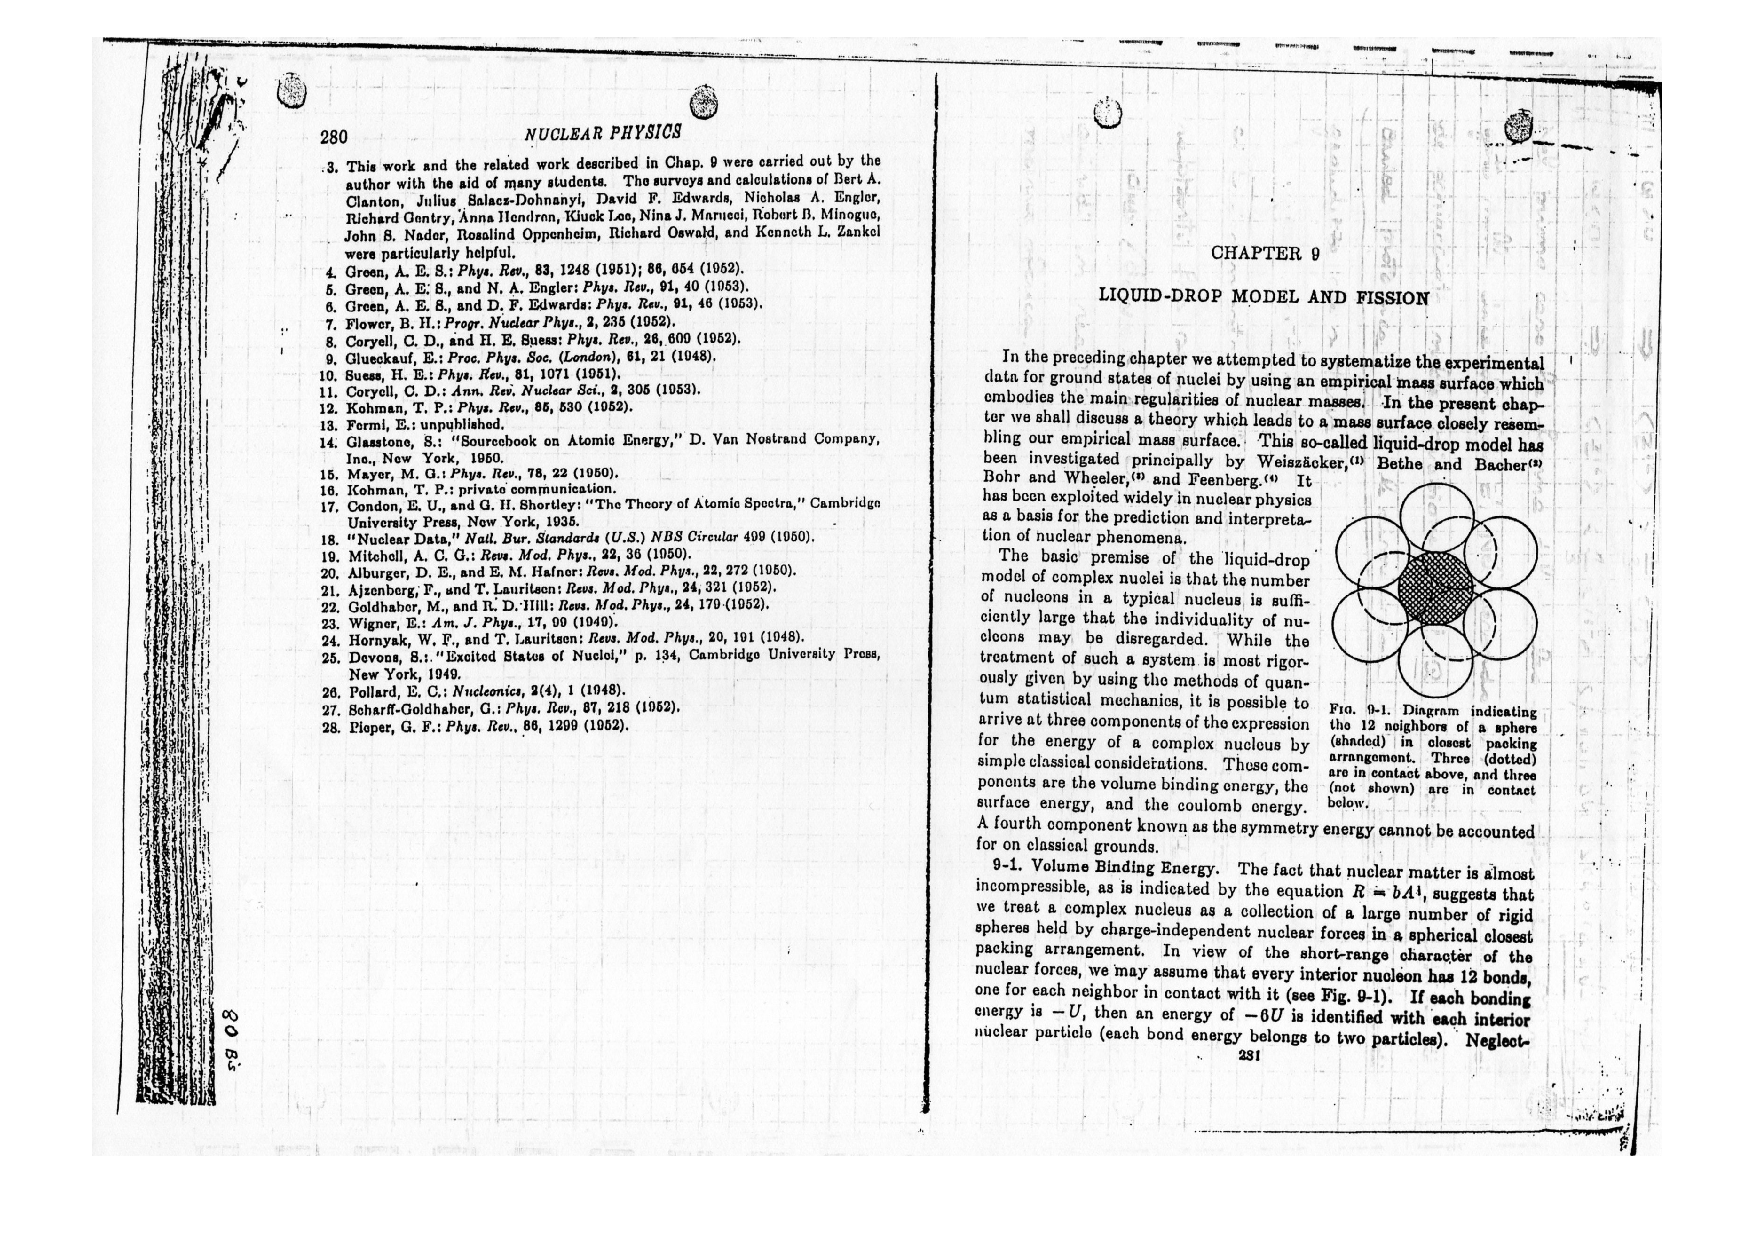
\includepdf[landscape,fitpaper=true,addtotoc={1,section,1,Allegato\
1,allegato_1}]{allegati/1.pdf}
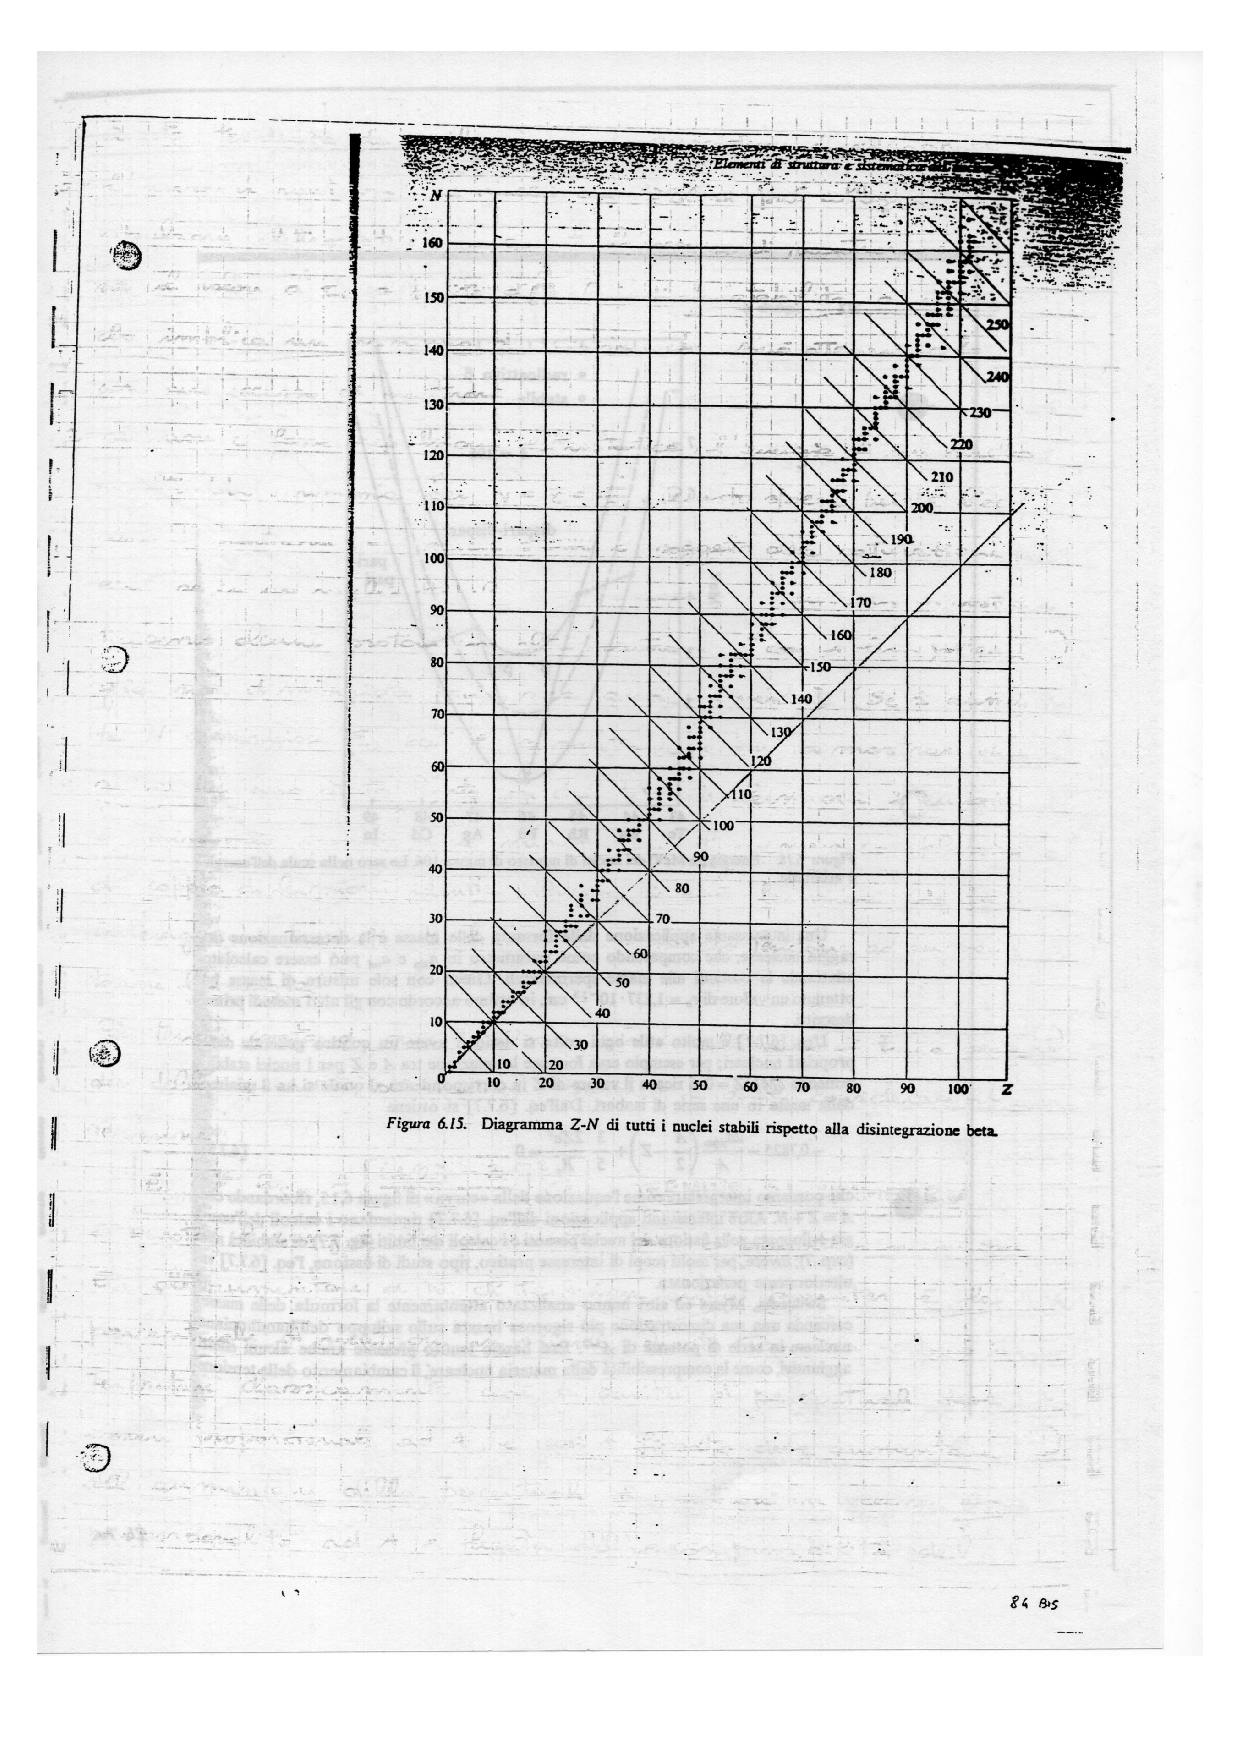
\includepdf[landscape,fitpaper=true,addtotoc={1,section,1,Allegato\
2,allegato_2}]{allegati/2.pdf}
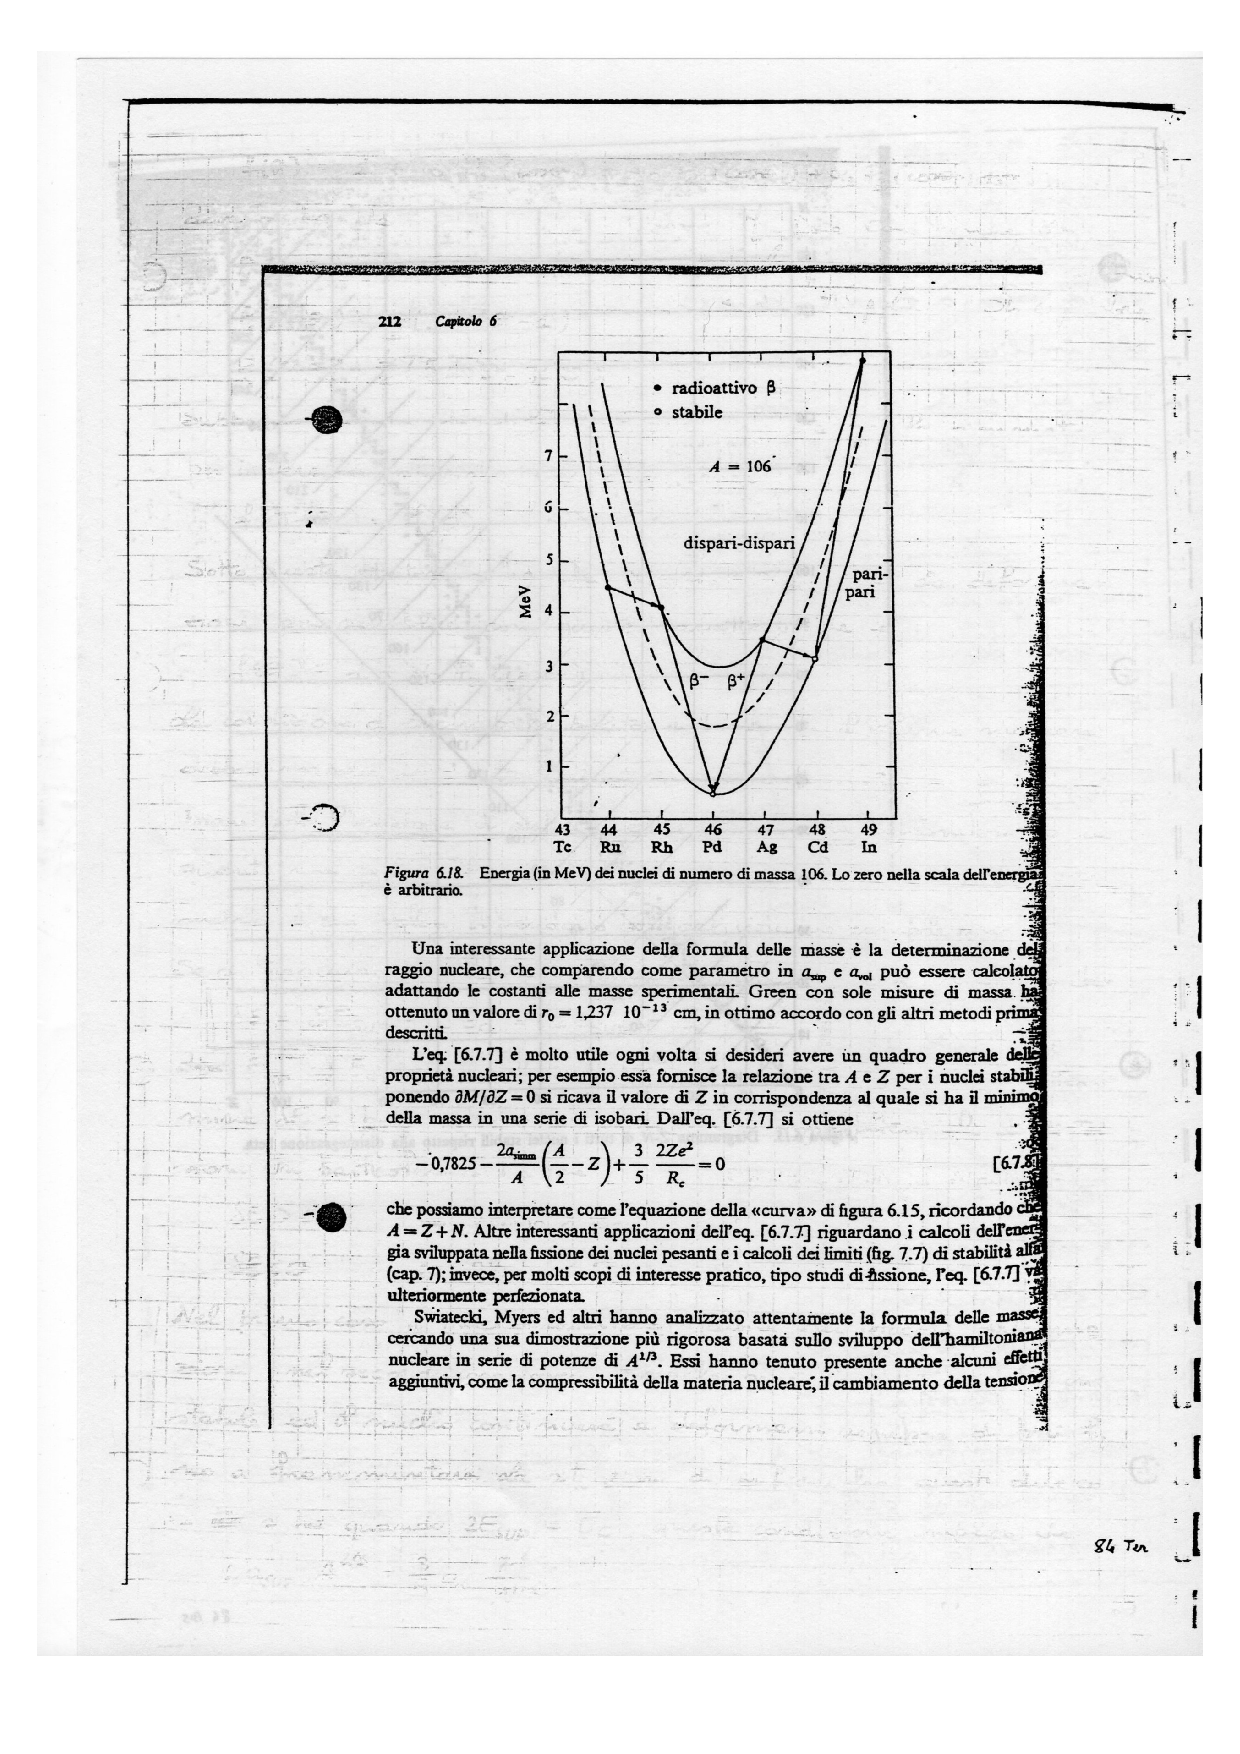
\includepdf[landscape,fitpaper=true,addtotoc={1,section,1,Allegato\
3,allegato_3}]{allegati/3.pdf}
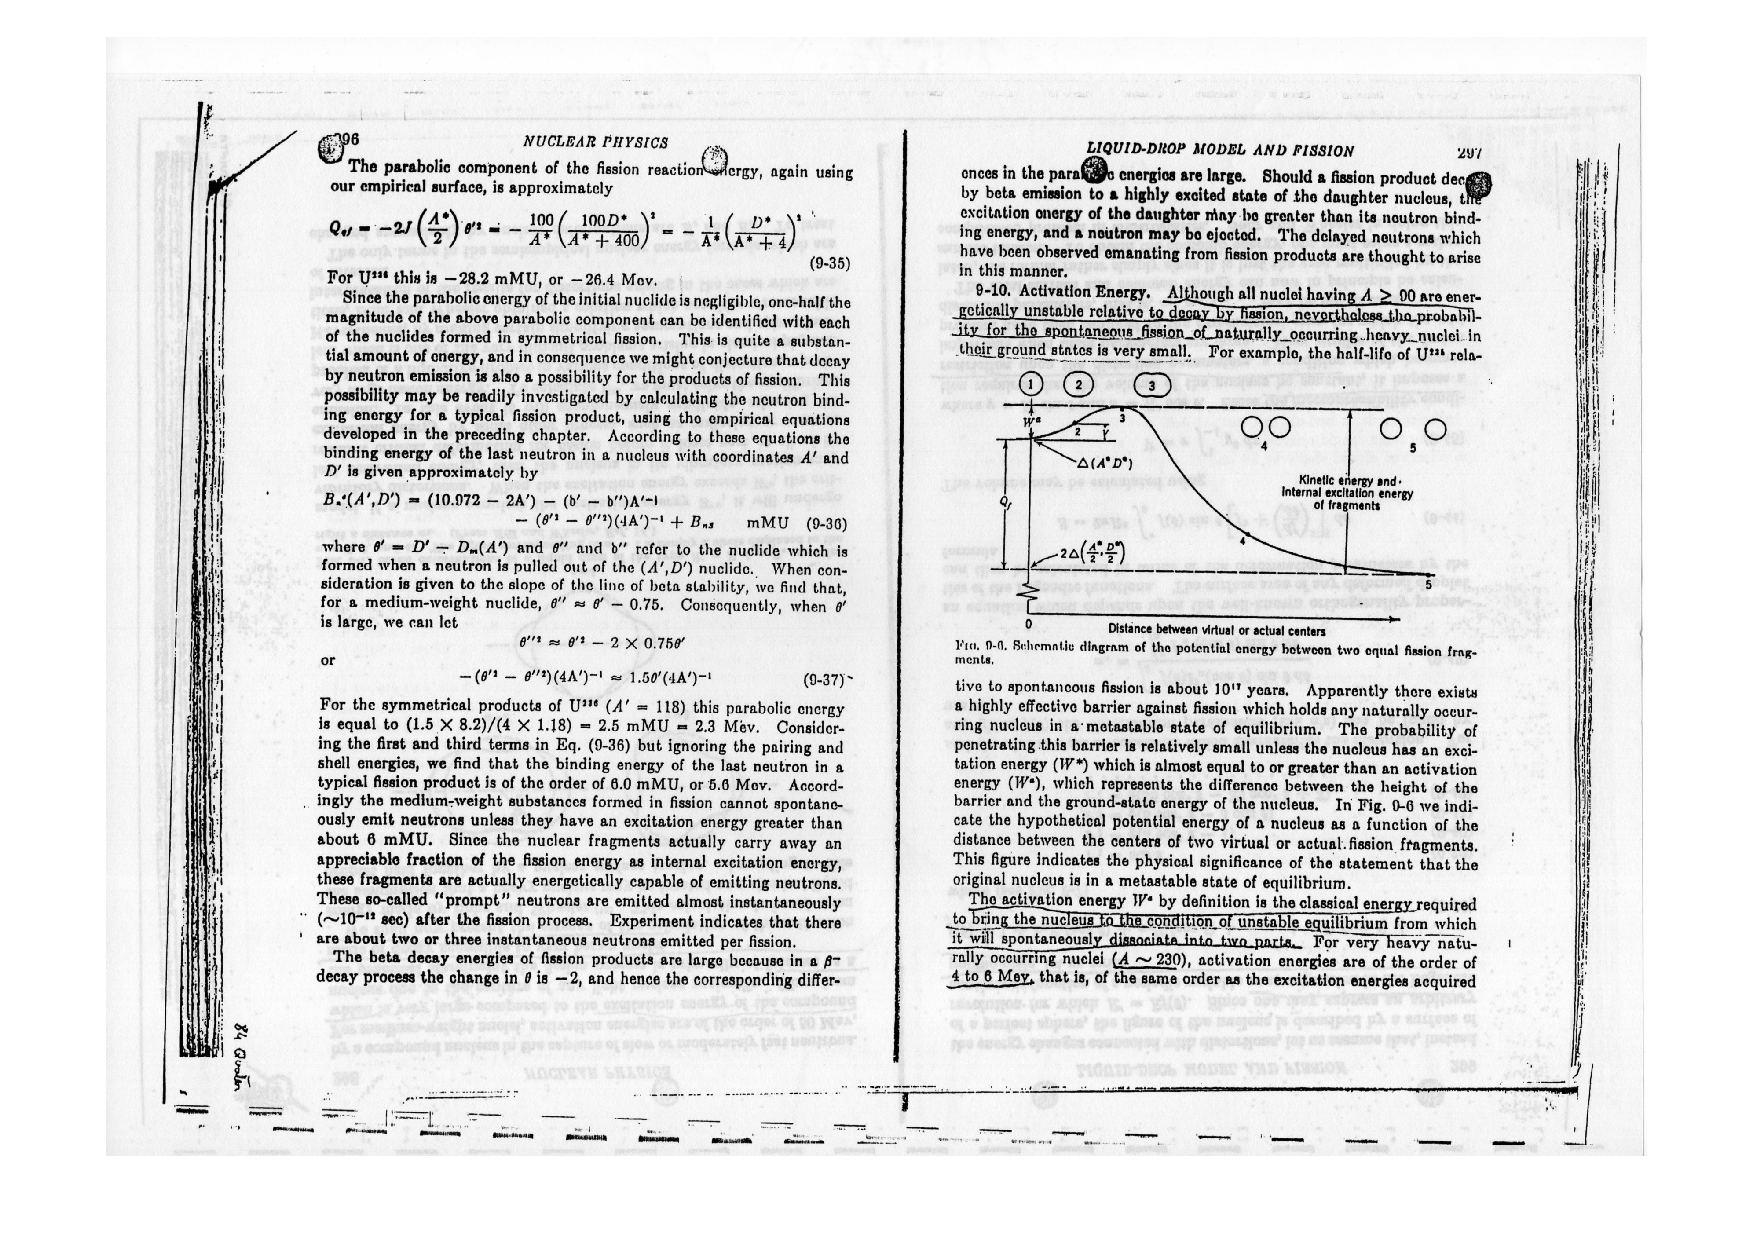
\includepdf[landscape,fitpaper=true,addtotoc={1,section,1,Allegato\
4(1),allegato_41}]{allegati/4_1.pdf}
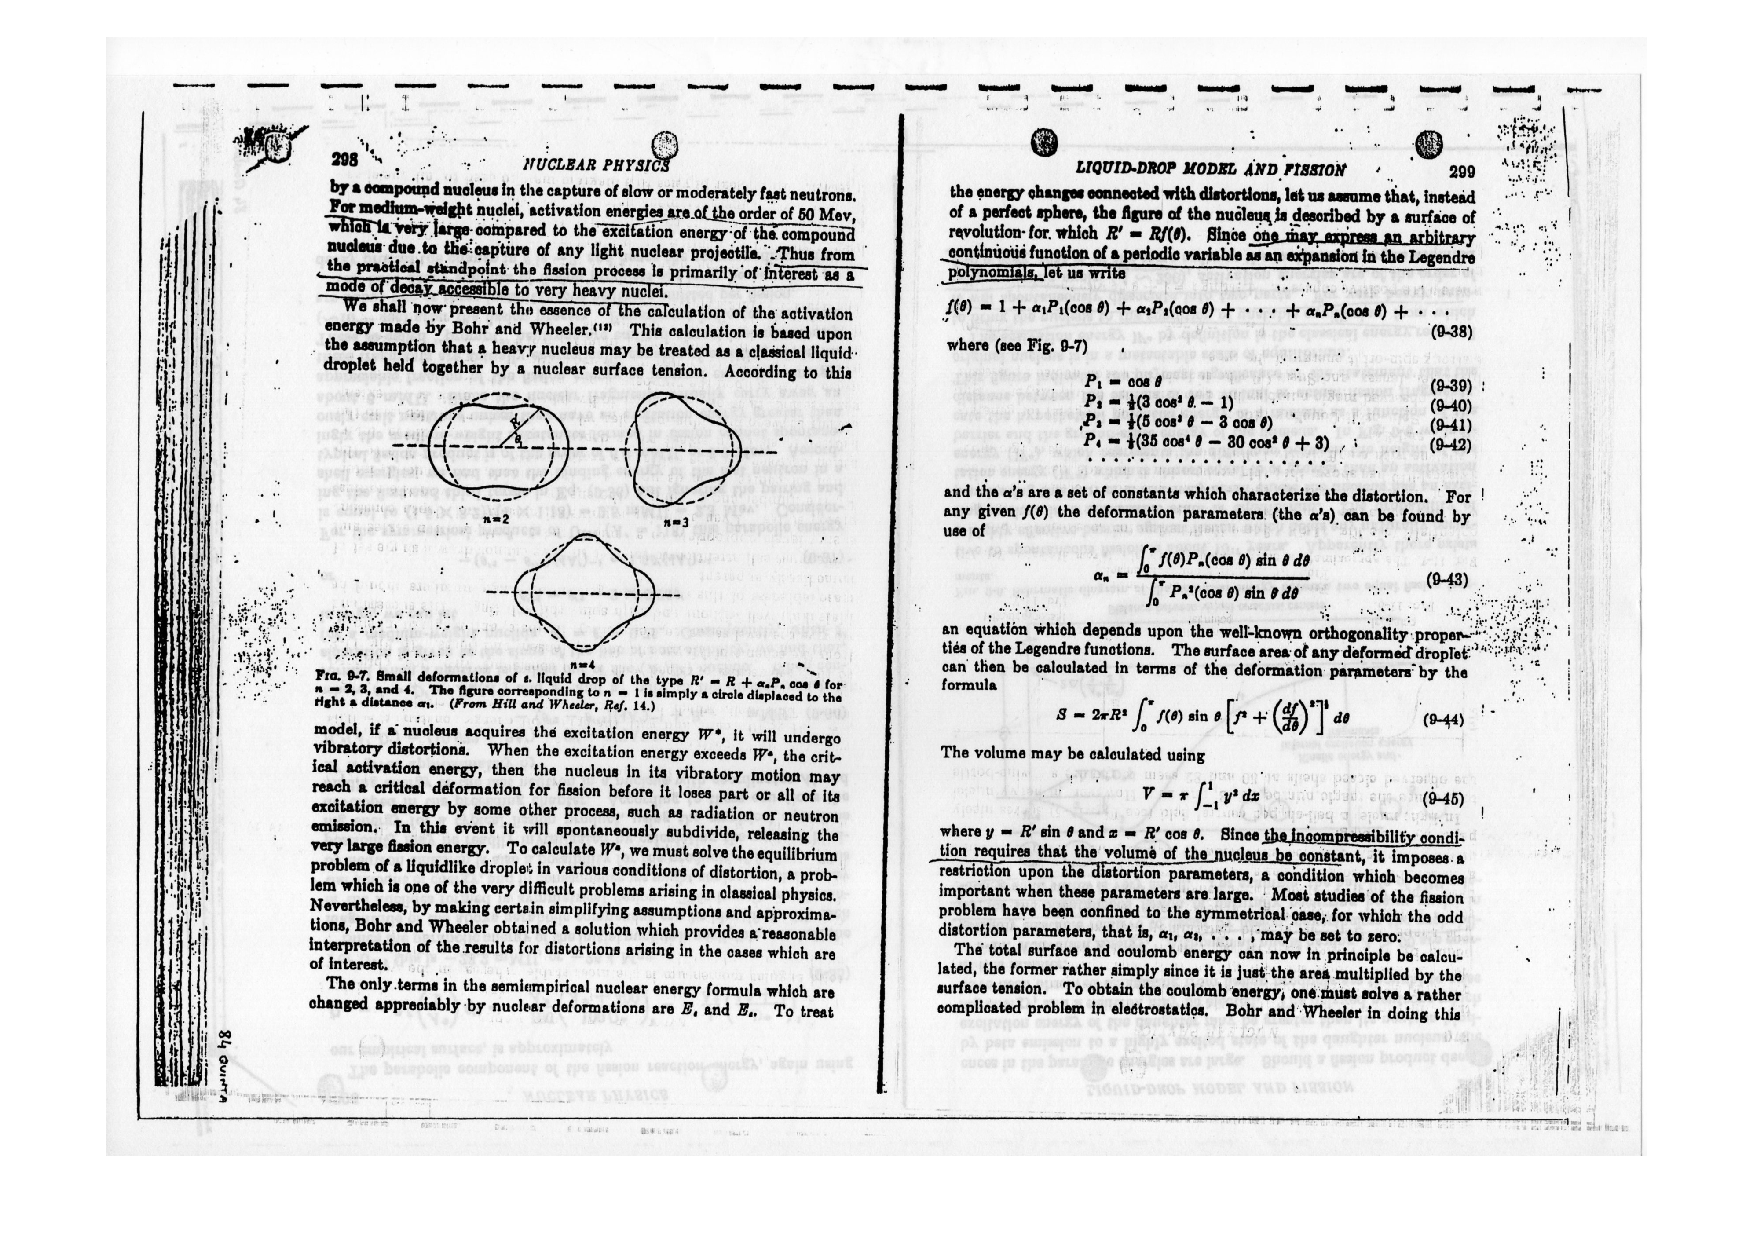
\includepdf[landscape,fitpaper=true,addtotoc={1,section,1,Allegato\
4(2),allegato_42}]{allegati/4_2.pdf}
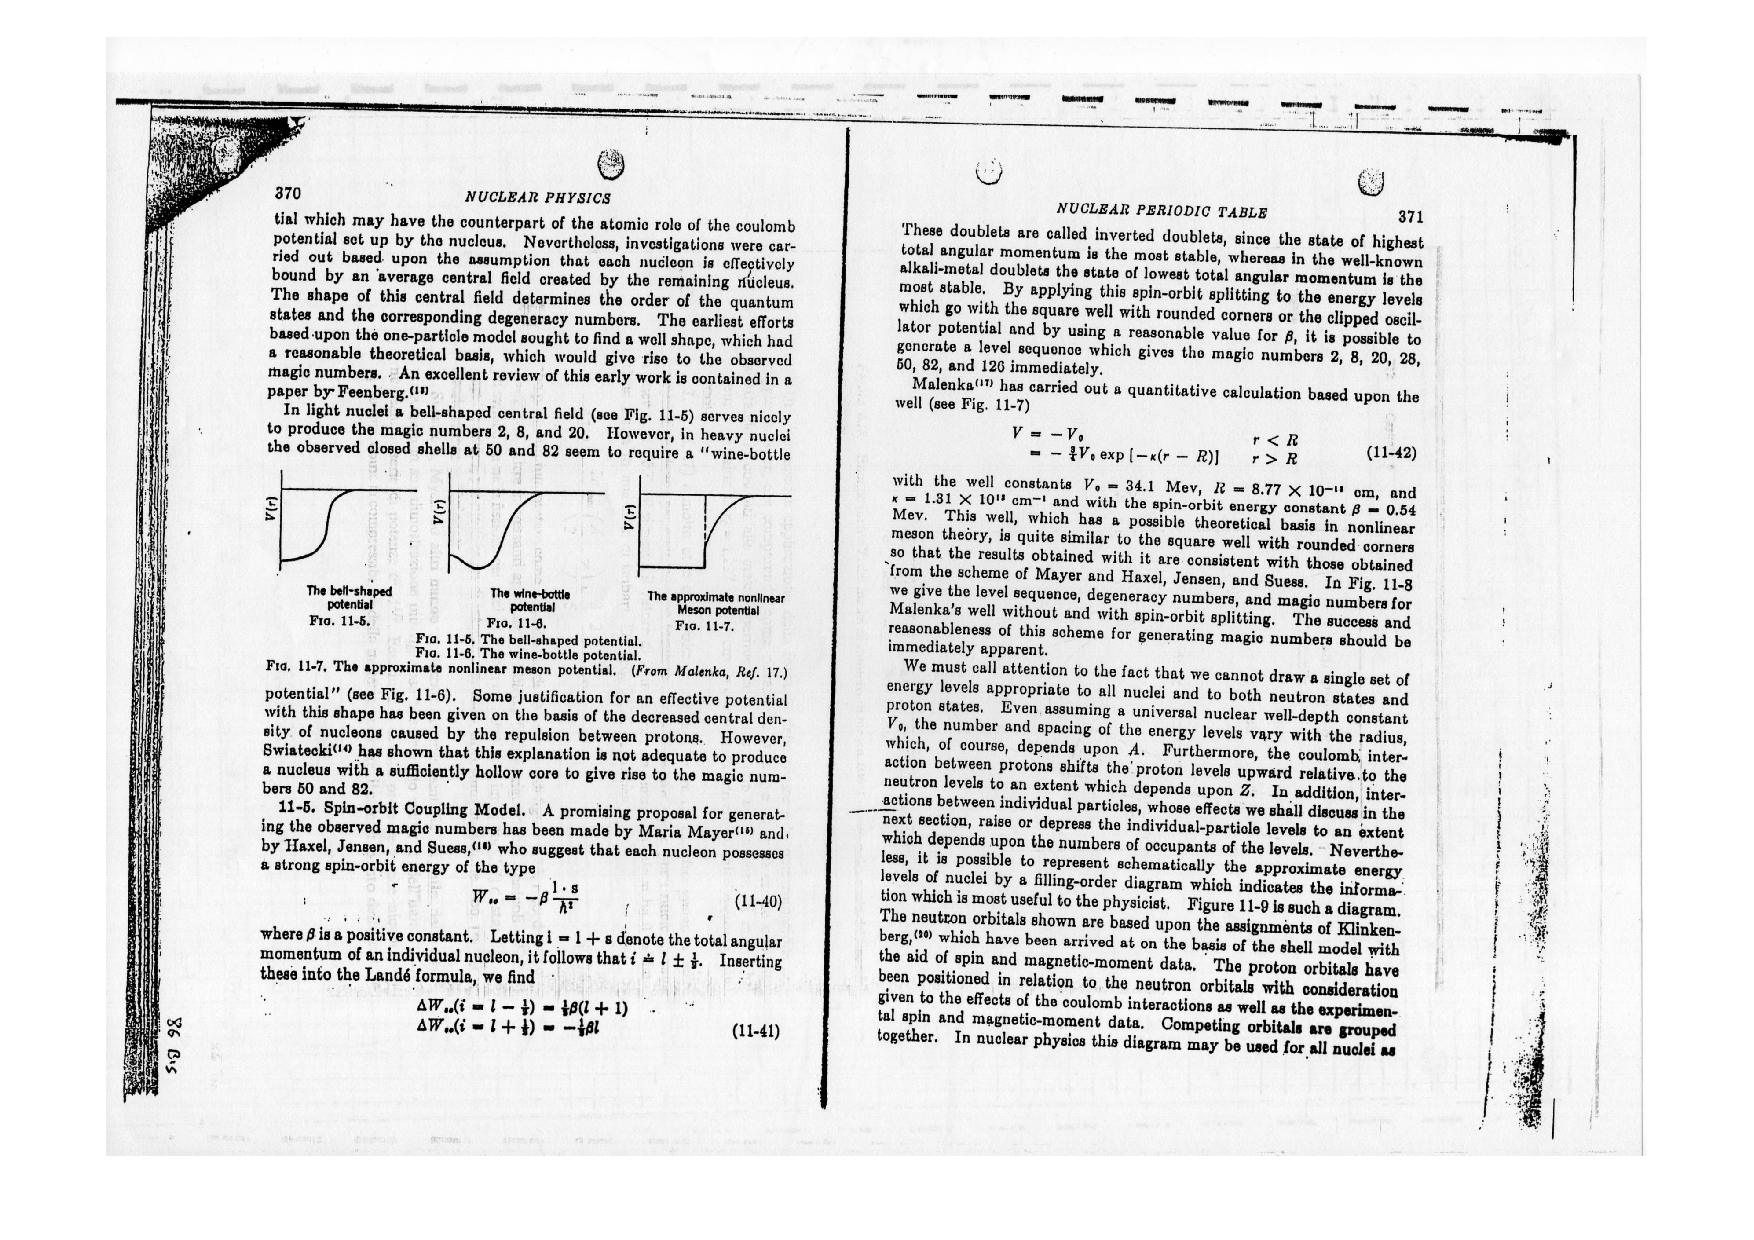
\includepdf[landscape,fitpaper=true,addtotoc={1,section,1,Allegato\
5,allegato_5}]{allegati/5.pdf}
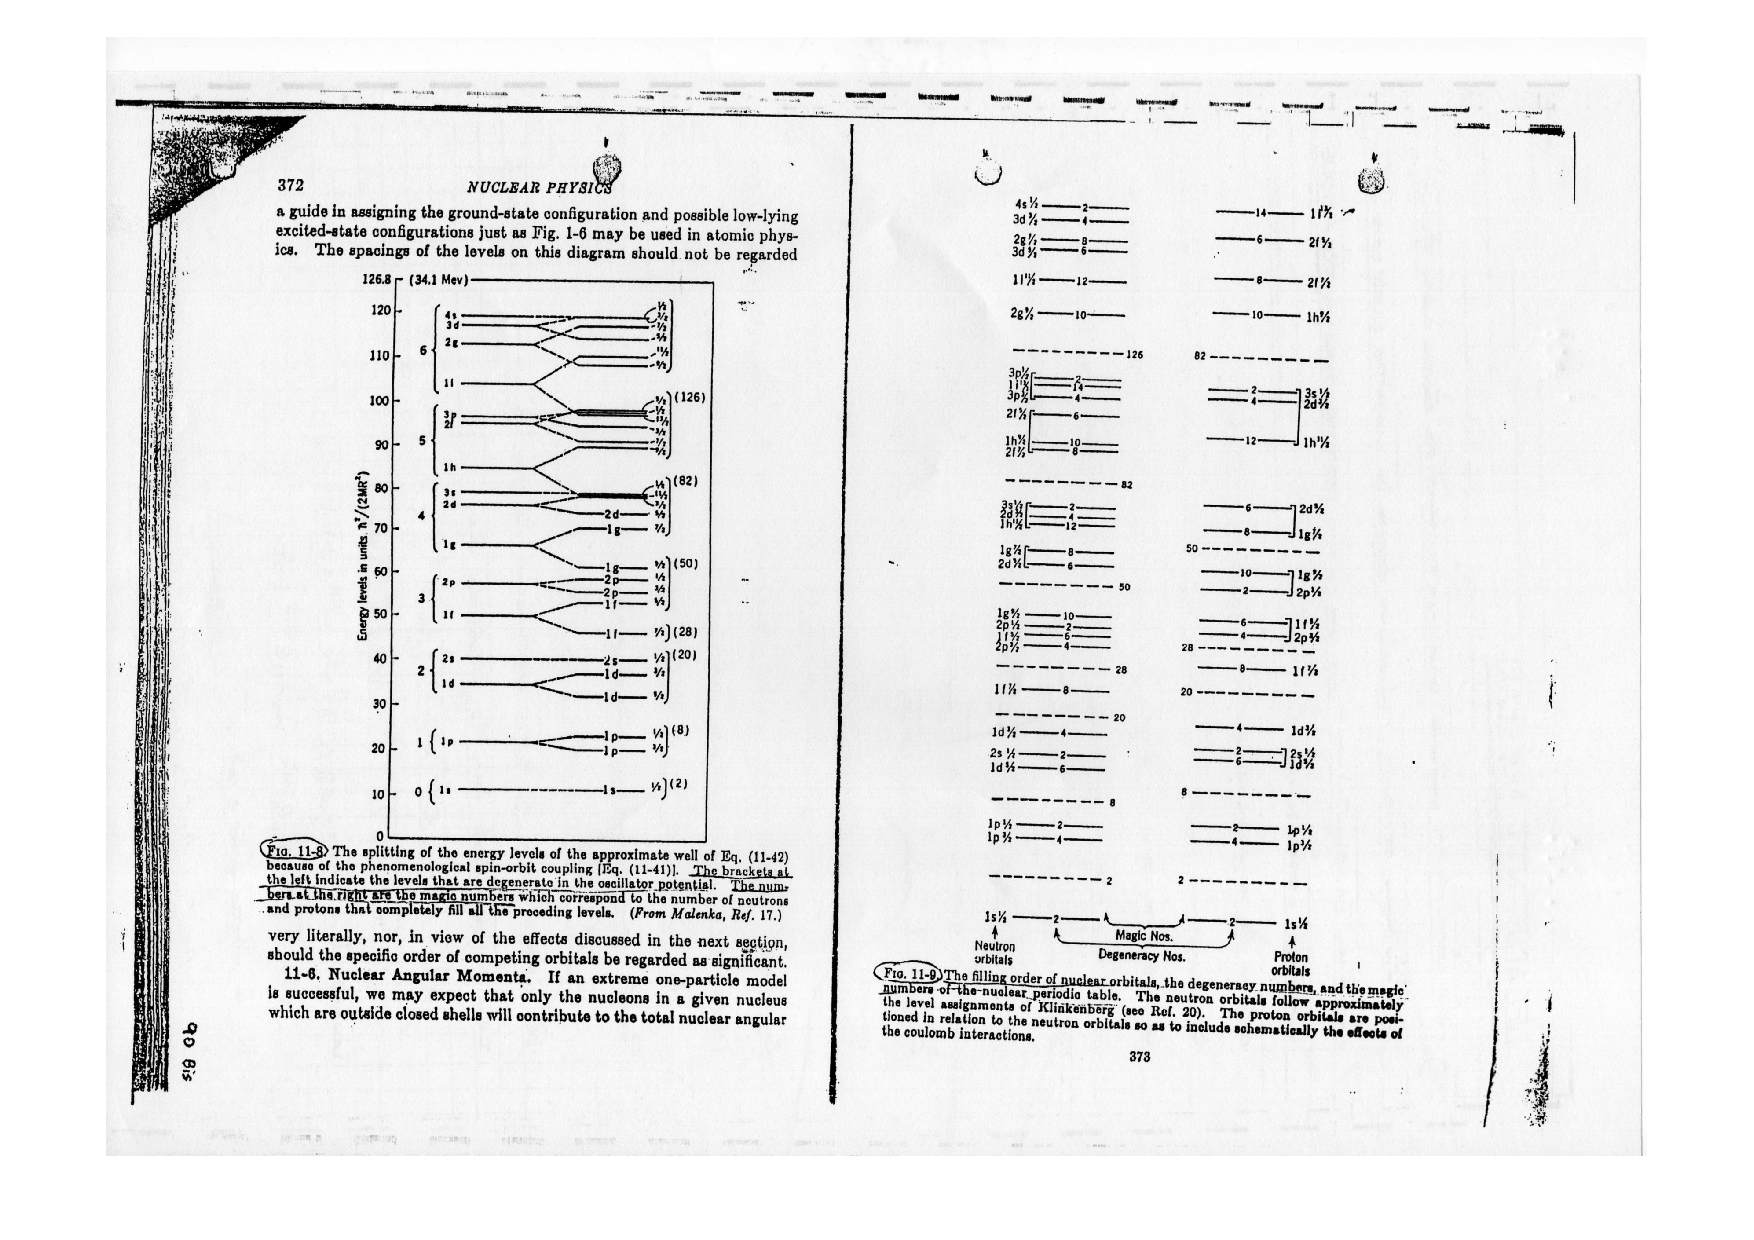
\includepdf[landscape,fitpaper=true,addtotoc={1,section,1,Allegato\
6,allegato_6}]{allegati/6.pdf}

\chapter{Riferimenti - Formule e costanti numeriche}
\section{Masse}
\begin{table}[!h]
  \centering
  \caption{Dati relativi alle masse.}
  \begin{tabular}{>{\scshape}lr}
	\toprule
    $\gamma - 1$ elettrone          & 2$\div$20\\
	$\gamma - 1$ protone/neutrone   & $< 1$\%\\
	Difetto di massa $^4$He         & $\simeq 28$ MeV\\
	U.m.a.                          & $\simeq 931,5$Mev/c$^2 = 11,66\cdot 10^{-24}$g\\
	Densità nucleare                & $10^{14}$g/cm$^3$\\
    \bottomrule
  \end{tabular}
\end{table}


\begin{table}[!h]
  \centering
  \caption{Massa particelle (in MeV/c$^2$, eccetto il neutrino)}
  \subfloat[][]{
	\begin{tabular}{>{\scshape}lr}
	  \toprule
	  Elettrone ($e$) & 0,5\\
	  Protone ($p$)   & 938 ovvero 1,0073 \textsc{um}\\
	  Neutrone ($n$)  & 939 ovvero 1,0087 \textsc{um}\\
	  \bottomrule
	\end{tabular}
  }\\
  \subfloat[][]{
	\begin{tabular}{>{\scshape}lr}
	  \toprule
	  Neutrino $\nu$     & < 60 eV\\
	  Muone ($\mu$)      & 105\\
	  Muone ($\mu^-$)    & 106\\
	  Pione ($\pi$)      & 138\\
	  Quark up ($u$)     & 336\\
	  Quark down ($d$)   & 336\\
	  	  \bottomrule
	\end{tabular}
  }
  \subfloat[][]{
	\begin{tabular}{>{\scshape}lr}
	  \toprule
	  Mesone $K^0$         & 497,7\\
	  Quark strange ($s$) & 538\\
	  Eta ($\eta$°)       & 549\\
	  Iperone $\Lambda$   & 1115,6\\
	  Quark charm ($c$)   & 1650\\
	  Tauone ($\tau$)     & 1782\\
	  \bottomrule
	\end{tabular}
  }
\end{table}
\section{Energie}
\begin{empheq}[box=\fbox]{align*}
  h &= 6,626\cdot 10^{-34}J\,s = 4,135\cdot 10^{-15}eV\,s\\
  \hslash &= \frac{h}{2\pi} = 1,054\cdot 10^{-34}J\,s = 6,582\cdot
  10^{-16}eV\,s\\
  1 eV &= 1,6\cdot 10^{-19}J = 1,6\cdot 10^{-12}\text{erg}\\
  e^- &= 1,6\cdot 10^{-19}C
\end{empheq}

\begin{table}[!h]
  \centering
  \caption{Energie di soglia di creazione}
  \begin{tabular}{>{\scshape}l>{$}r<{$}}
	\toprule
	Elettrone-Positrone & \simeq 1,022 \text{MeV}\\
	Protone-Antiprotone & \simeq 1,9 \text{GeV}\\
	\bottomrule
  \end{tabular}
\end{table}

\begin{table}[!h]
  \centering
  \caption{Energia dei fotoni}
  \begin{tabular}{>{\scshape}rl}
	\toprule
	Microonde & $\sim$ 1 meV\\
	IR        & $\sim$ 1 eV\\
	Visibile  & $\sim$ 10 eV\\
	UV        & $\sim$ 1 keV\\
	Soft-X    & $\sim$ 10 keV\\
	Hard-X    & $\sim$ 1-100 MeV\\
	$\gamma$  & $\sim$ >100 MeV\\
	\bottomrule
  \end{tabular}
\end{table}

\section{Miscellanea}
\begin{description}
  \item[Sezione d'urto tipica] centibarn - barn (1 barn = $10^{-24}$ m$^2$)
  \item[Parametro d'urto esperimento di Rutherford] $p(\theta)_\text{min} =
	10^{-13}$cm e $p(\theta)_\text{max} = 10^{-8}$cm
  \item[$R$ parametro d'urto minimo] $R = r_0A^{1/3}$ dove $A$ è il numero
	atomico e $r_0 \simeq 1,2\cdot 10^{-13}$cm
  \item[Lunghezza d'onda elettronica] $E = 1$ GeV
	$\rightarrow$\textcrlambda$\simeq 1,95\cdot 10^{-14}$cm
  \item[Magnetone nucleare] $\mu_N = \dfrac{e\hslash}{2m_pc}\simeq
	0,505\cdot 10^{-23}$erg/gauss
\end{description}

\section{Formule}
\begin{description}
  \item[Energia di soglia]
	\begin{equation}
	  E_s = \frac{M_\text{min}^2 - M^2 - m^2}{2M}c^2
	\end{equation}
  \item[Energia di legame]
	\begin{equation}
	  \Delta E_0 = (E_{01} + E_{02}) - E_0 = \Delta M c^2
	\end{equation}
  \item[Sezione d'urto di Rutherford]
	\begin{equation}
	  \frac{\text{d}\sigma}{\text{d}\Omega} =
	  \frac{1}{4}\left[\frac{Ze(2e)^2}{m_\alpha v^2}\right]^2
	  \frac{1}{\sin^4(\theta/2)}
	\end{equation}
  \item[Frazione di impacchettamento]
	\begin{equation}
	  f = \frac{M(A,Z) - A\,UM}{A\,UM}
	\end{equation}
  \item[Fattore di forma] 
	\begin{gather}
	  \abs{F}^2 = \frac{\abs{f(\theta)}^2}{\abs{f_0(\theta)}^2}\\
	  F = F(\vec{q}) = \int \rho(\vec{r})e^{i\vec{q}\cdot\vec{r}}\text{d}^3r
	\end{gather}
  \item[Formula di Saxon] $c = 1,07A^{1/3}\cdot 10^{-13}$cm, $Z_1 = 0,545\cdot
	10^{-13}$cm, $\rho_1 =$ costante di normalizzazione
	\begin{equation}
	  \rho(r) = \frac{\rho_1}{e^{(r-c)/Z_1}+1}
	\end{equation}
  \item[Momento magnetico nucleare]
	\begin{equation}
	  \vec{\mu}_I = \frac{g_I\mu_N\vec{I}}{\hslash} = \gamma \vec{I}
	\end{equation}
  \item[Regola degli intervalli] 
	\begin{equation}
	  \frac{W_\alpha-W_{\alpha+1}}{W_{\alpha+1}-W_{\alpha+2}} =
	  f_\alpha/f_{\alpha+1}
	\end{equation}
  \item[Momento di quadrupolo elettrico del nucleo]
	\begin{equation}
	  Q = \int \rho_c^N(3Z^{\prime 2}-r^2)\text{d}V
	\end{equation}
  \item[Energia elettrostatica dovuta al quadrupolo]
	\begin{equation}
	  \Delta W = \frac{1}{4}\frac{\partial^2\varphi}{\partial
	  Z^2}Q\left( \frac{3}{2}\cos^2(\theta) - \frac{1}{2} \right)
	\end{equation}
  \item[Energia di quadrupolo elettrico semiclassica]
	\begin{equation}
	  \Delta W_Q = \frac{1}{4}\frac{\partial^2\varphi}{\partial Z^2}Q\left(
	  \frac{3}{2}K_f^2-2i^2j^2 \right)\frac{1}{4i^2j^2}
	\end{equation}
  \item[Energia di quadrupolo eletrico quantistica]
	\begin{equation}
	  \Delta W_Q = \frac{1}{4}\frac{\partial^2 \varphi}{\partial Z^2}Q\left(
	  \frac{3}{2}K_f(K_f+1)-2i(i+1)j(j+1)
	  \right)\frac{1}{i(2i-1)j(2j-1)}
	\end{equation}
  \item[Formula di Weizs\"acker] $a_\text{vol}=15,67\quad a_\text{sup} =
	17,23\quad 3a_c/5 = 0,7\quad a_\text{simm} = 93,15\quad \delta = 1,2$
	\begin{multline}
	  M(A,Z) = \left[ m_pZ + m_N(A-Z) \right] -a_\text{vol}A +
	  a_\text{sup}A^{2/3}+\\
	  +\frac{3}{5}a_c\frac{Z^2}{A^{1/3}} +
	  a_\text{simm}\frac{(A/2-Z)^2}{A} + \frac{\delta}{a^{1/2}}
	\end{multline}
  \item[Fattore di Gamow]
	\begin{equation}
	  G(T_\alpha,Z',R') =
	  \frac{2e^2Z'}{\hslash}\sqrt{\frac{2m_\alpha}{T_\alpha}} =
	  \frac{4}{\hslash}\sqrt{m_\alpha Z'R'}
	\end{equation}
  \item[Regola d'oro di Fermi]
	\begin{equation}
	  W = \frac{2\pi}{\hslash}\abs{H_{if}}^2\rho_f(E_i)\qquad \rho_f(E_i) =
	  \left.\frac{\text{d}N}{\text{d}E_f}\right|_{E_f=E_i}
	\end{equation}
  \item[Sezione d'urto di produzione della risonanza (no spin)]
	\begin{equation}
	  G^{(\ell)} = \frac{4\pi}{K^2_R}(2\ell +
	  1)\frac{\Gamma^2/4}{(E-E_R)^2+\Gamma^2/4}
	\end{equation}
  \item[Sezione d'urto di produzione della risonanza (con spin)]
	\begin{equation}
	  G^{(\ell)} = \frac{4\pi}{K^2_R}
	  \frac{(2J_R + 1)}{(2S_a + 1)(2S_b + 1)}\frac{\Gamma^2/4}{(E-E_R)^2+\Gamma^2/4}
	\end{equation}
\end{description}
\section{Reazioni nucleari}
\begin{table}[!h]
  \centering
  \caption{Alcune reazioni basilari.}
  \begin{tabularx}{\textwidth}{>{$}r<{$}X}
	\toprule
	\gamma + N \rightarrow e^+ + e^- + N & Creazione coppia elettrone -
	positrone\\
	n + p \rightarrow d + \gamma & Reazione usata per misurare la massa di $n$
	($d$ è il deutone)\\
	\text{U}^{238} \rightarrow \text{Th}^{234} + \alpha & $T_\alpha\simeq 4,2$ MeV\\
	N(A,Z) \rightarrow N(A,Z+1) + e^- + \bar{\nu}\quad(n\rightarrow p^+) &
	Decadimento $\beta^-$\\
    N(A,Z) \rightarrow N(A,Z-1) + e^+ + \nu\quad(p^+\rightarrow n) &
	Decadimento $\beta^+$\\
	p^+ + e^- \rightarrow n + \nu & Processo di cattura $K$\\
	\pi^- + p^+ \rightarrow \Lambda^0 + K^0 & Processo di produzione (associata)
	di $\Lambda^0$ e $K^0$\\
	\Lambda^0 \rightarrow  p^+ + \pi^-,\quad K^0 \rightarrow \pi^+ + \pi^- &
	Decadimenti deboli di $\Lambda^0$ e $K^0$\\
	\pi^- + p^+ \rightarrow K^+ + K^- + n & Processo di produzione di $K^+$\\
	K^- + p^+ \rightarrow \bar{K}^0 + n & Produzione di $\bar{K}^0$\\
	K^- + N \rightarrow \pi + \Lambda^0, \quad K^- + N \rightarrow \pi + \Sigma &
	Assorbimento del mesone $K^-$\\
	Kì- + p^+ \rightarrow \eta^0 + \Lambda^0 & Produzione del mesone $\eta^0$\\
	\pi^- \rightarrow \mu^- + \bar{\nu}_\mu & Produzione del muone\\
	\mu^- \rightarrow e^- + \bar{\nu}_e + \nu_{\mu} & Decadimento debole del
	muone\\
	\bottomrule
  \end{tabularx}
\end{table}

\begin{table}[!h]
  \centering
  \caption{Processi di produzione mesone $\pi$}
  \begin{tabular}{>{$}l<{$}|>{$}c<{$}|>{$}r<{$}}
	\toprule
	p^+ + p^+ \rightarrow p^+ + p^+ + \pi^0 & n + p^+ \rightarrow n + p^+ +
	\pi^0 & p^+ + n \rightarrow d + \pi^0\\
    p^+ + p^+ \rightarrow p^+ + n + \pi^+ & n + p^+ \rightarrow p^+ + p^+ +
	\pi^- & \gamma + p^+ \rightarrow p^+ + \pi^0\\
    p^+ + p^+ \rightarrow d + \pi^+ & n + p^+ \rightarrow n + n + \pi^+ & \gamma
	+ p^+ \rightarrow n + \pi^+\\
	\bottomrule
  \end{tabular}
\end{table}

\begin{table}[!h]
  \centering
  \caption{Processi di produzione degli iperoni}
  \begin{tabular}{>{$}l<{$}|>{$}c<{$}|>{$}r<{$}}
	\toprule
	K^- + p^+ \rightarrow \pi^+ + \Sigma^- &K^- + p^+ \rightarrow \pi^0 +
	\Sigma^0 &K^- + p^+ \rightarrow \pi^0 + \Sigma^+\\
    K^- + p^+ \rightarrow K^+ + \Xi^- &K^- + p^+ \rightarrow K^0 + \Xi^0 &K^- + p^+
	\rightarrow K^0 + \Omega^- + K^+ \\
	\bottomrule
  \end{tabular}
\end{table}

\begin{table}[!h]
  \centering
  \caption{Processi di decadimento (non leptonici) del mesone $K^+$}
  \begin{tabular}{>{$}l<{$}|>{$}c<{$}|>{$}r<{$}}
	\toprule
  K^+ \rightarrow \pi^+ + \pi^0 & K^+ \rightarrow \pi^+ + \pi^+ + \pi^- & K^+
  \rightarrow \pi^+ + \pi^0 + \pi^0\\
	\bottomrule
  \end{tabular}
\end{table}

\end{document}
